%%____________________________________________________________________________||
\section{Results}
\label{sec:results}

In this section the main results concerning the fit are summarised. 

Tables ~\ref{tab:predall_sig_comb_mono}-~\ref{tab:predall_sig_comb_asym} summarise the predicted and observed yields in the signal region for ``symmetric'' and ``asymmetric'' topologies respectively, 
corresponding to an integrated luminosity of 1.26 \ifb.
The predicted yields are based on a fit to multiple data control samples to obtain predictions in (\nj,\nb,\scalht). 
The observed counts in the signal region are not considered in this fit. 
The uncertainties reflect all statistical and (pre-fit) systematic sources added in quadrature. 
The $\ttbar$W and \znunu components are also shown (the former of which contains all residual contributions from sub-dominant processes such as e.g. diboson production). 
This table summarises our best knowledge of the SM background rates in the signal region while not considering counts in the signal region itself. 

\begin{table}[h!]
\tiny
\centering
\caption{Pre fit Predictions and Data in the signal region for 12.9\ifb for monojet categories. All entries are non-zero but are truncated to one decimal place.\label{tab:predall_sig_comb_mono}}
\scalebox{0.85}{\begin{tabular}{cccccccccc}
	\hline\hline
	&	& \multicolumn{8}{c}{\scalht (\gev)}\\ 
	&	 (\njet, \nb) & 200-250 & 250-300 & 300-350 & 350-400 & 400-500 & 500-600 & 600-800 & 800-$\infty$ \\ [0.8ex] 
\hline
	Data & (1, 0) & 70743 & 23504 & 8886 & 3692 & 2596 & 663 & 339 & -- \\[0.5ex] 
	SM & (1, 0) & $63535.9\pm 2676.7$ & $20393.7\pm 1429.9$ & $8249.7\pm 466.5$ & $3428.5\pm 394.9$ & $2255.0\pm 269.7$ & $583.5\pm 33.3$ & $398.9\pm 130.0$ & -- \\[0.5ex] 
	Ttw & (1, 0) & $28420.4\pm 1197.0$ & $8148.4\pm 571.3$ & $3007.0\pm 170.8$ & $1160.9\pm 133.6$ & $683.3\pm 81.9$ & $155.6\pm 9.1$ & $100.2\pm 32.7$ & -- \\[0.5ex] 
	Zinv & (1, 0) & $35113.6\pm 1480.2$ & $12245.3\pm 858.6$ & $5240.8\pm 295.8$ & $2267.3\pm 261.3$ & $1571.6\pm 187.8$ & $424.3\pm 23.9$ & $297.8\pm 97.2$ & -- \\[0.5ex] 
	Data & (1, 1) & 2704 & 927 & 378 & 154 & 111 & 78 & -- & -- \\[0.5ex] 
	SM & (1, 1) & $2599.6\pm 129.6$ & $892.7\pm 60.8$ & $351.4\pm 33.2$ & $145.4\pm 23.6$ & $116.1\pm 9.0$ & $53.7\pm 5.7$ & -- & -- \\[0.5ex] 
	Ttw & (1, 1) & $937.6\pm 46.6$ & $314.0\pm 21.4$ & $117.1\pm 11.0$ & $38.6\pm 6.3$ & $43.5\pm 3.4$ & $14.2\pm 1.6$ & -- & -- \\[0.5ex] 
	Zinv & (1, 1) & $1662.0\pm 83.2$ & $578.7\pm 39.4$ & $234.3\pm 22.2$ & $106.8\pm 17.3$ & $72.6\pm 5.6$ & $39.2\pm 4.2$ & -- & -- \\[0.5ex] 
	\hline
	\hline
\end{tabular}}
\end{table}

\begin{table}[h!]
\tiny
\centering
\caption{Pre fit Predictions and Data in the signal region for 2.2\ifb for symmetric categories. All entries are non-zero but are truncated to one decimal place.\label{tab:predall_sig_comb_sym}}
\scalebox{0.85}{\begin{tabular}{cccccccccc}
	\hline\hline
	&	& \multicolumn{8}{c}{\scalht (\gev)}\\ 
	&	 (\njet, \nb) & 200-250 & 250-300 & 300-350 & 350-400 & 400-500 & 500-600 & 600-800 & 800-$\infty$ \\ [0.8ex] 
\hline
	Data & (2, 0) & 1167 & 1155 & 760 & 442 & 335 & 119 & 58 & 57 \\[0.5ex] 
	SM & (2, 0) & $1104.5\pm 248.2$ & $1156.7\pm 196.1$ & $756.9\pm 92.7$ & $417.8\pm 50.2$ & $354.8\pm 47.2$ & $117.5\pm 21.8$ & $48.5\pm 8.1$ & $57.8\pm 13.8$ \\[0.5ex] 
	Ttw & (2, 0) & $516.4\pm 127.7$ & $519.3\pm 87.2$ & $325.2\pm 42.4$ & $158.8\pm 33.7$ & $127.8\pm 26.9$ & $39.7\pm 8.4$ & $14.8\pm 3.3$ & $18.2\pm 4.5$ \\[0.5ex] 
	Zinv & (2, 0) & $535.4\pm 131.8$ & $610.4\pm 133.9$ & $409.5\pm 55.3$ & $237.5\pm 26.9$ & $214.2\pm 31.0$ & $76.4\pm 15.7$ & $33.7\pm 6.1$ & $39.5\pm 10.1$ \\[0.5ex] 
	Data & (2, 1) & 137 & 115 & 76 & 40 & 39 & 5 & 4 & 2 \\[0.5ex] 
	SM & (2, 1) & $112.7\pm 25.7$ & $91.0\pm 15.8$ & $53.3\pm 8.2$ & $31.6\pm 4.8$ & $31.3\pm 4.6$ & $12.0\pm 2.4$ & $4.9\pm 0.9$ & $4.4\pm 1.3$ \\[0.5ex] 
	Ttw & (2, 1) & $69.0\pm 17.3$ & $47.7\pm 8.9$ & $24.6\pm 4.4$ & $11.5\pm 2.8$ & $10.5\pm 2.3$ & $4.0\pm 0.9$ & $1.3\pm 0.3$ & $1.3\pm 0.4$ \\[0.5ex] 
	Zinv & (2, 1) & $38.3\pm 9.6$ & $41.2\pm 9.1$ & $27.1\pm 4.4$ & $18.5\pm 2.6$ & $19.6\pm 3.0$ & $7.8\pm 1.7$ & $3.6\pm 0.7$ & $3.1\pm 0.9$ \\[0.5ex] 
	Data & (2, 2) & 8 & 6 & 3 & 5 & 3 & 0 & 0 & -- \\[0.5ex] 
	SM & (2, 2) & $5.6\pm 1.3$ & $3.5\pm 0.7$ & $7.1\pm 1.3$ & $1.1\pm 0.2$ & $1.3\pm 0.2$ & $1.5\pm 0.5$ & $0.3\pm 0.1$ & -- \\[0.5ex] 
	Ttw & (2, 2) & $2.7\pm 0.7$ & $1.5\pm 0.3$ & $3.9\pm 0.9$ & $0.4\pm 0.1$ & $0.5\pm 0.1$ & $1.0\pm 0.4$ & $0.1\pm 0.0$ & -- \\[0.5ex] 
	Zinv & (2, 2) & $2.7\pm 0.7$ & $2.0\pm 0.5$ & $3.0\pm 0.5$ & $0.6\pm 0.1$ & $0.8\pm 0.2$ & $0.5\pm 0.2$ & $0.2\pm 0.1$ & -- \\[0.5ex] 
	Data & (3, 0) & 4 & 205 & 592 & 577 & 624 & 215 & 97 & 79 \\[0.5ex] 
	SM & (3, 0) & $0.9\pm 0.3$ & $225.8\pm 39.6$ & $639.8\pm 82.5$ & $535.5\pm 81.8$ & $614.1\pm 79.1$ & $213.5\pm 38.9$ & $103.5\pm 17.8$ & $78.0\pm 18.5$ \\[0.5ex] 
	Ttw & (3, 0) & $0.6\pm 0.2$ & $105.4\pm 18.0$ & $305.5\pm 42.6$ & $238.5\pm 50.8$ & $257.9\pm 52.4$ & $80.8\pm 17.1$ & $34.2\pm 7.5$ & $23.8\pm 6.0$ \\[0.5ex] 
	Zinv & (3, 0) & $0.4\pm 0.2$ & $114.8\pm 26.5$ & $299.5\pm 43.2$ & $254.8\pm 32.3$ & $332.8\pm 48.6$ & $126.2\pm 25.8$ & $69.3\pm 12.9$ & $52.4\pm 13.3$ \\[0.5ex] 
	Data & (3, 1) & -- & 46 & 114 & 114 & 93 & 32 & 18 & 10 \\[0.5ex] 
	SM & (3, 1) & -- & $47.2\pm 8.3$ & $107.8\pm 17.2$ & $123.1\pm 22.6$ & $125.2\pm 18.7$ & $33.8\pm 6.6$ & $20.8\pm 3.7$ & $11.7\pm 3.1$ \\[0.5ex] 
	Ttw & (3, 1) & -- & $34.9\pm 6.6$ & $72.8\pm 13.8$ & $75.1\pm 18.2$ & $70.2\pm 15.4$ & $16.7\pm 3.9$ & $8.1\pm 1.9$ & $3.8\pm 1.1$ \\[0.5ex] 
	Zinv & (3, 1) & -- & $11.2\pm 2.6$ & $29.2\pm 4.6$ & $38.3\pm 5.4$ & $50.2\pm 7.5$ & $16.1\pm 3.4$ & $12.8\pm 2.5$ & $7.7\pm 2.2$ \\[0.5ex] 
	Data & (3, 2) & -- & 11 & 12 & 14 & 16 & 5 & 1 & 1 \\[0.5ex] 
	SM & (3, 2) & -- & $7.1\pm 1.3$ & $23.0\pm 4.4$ & $24.4\pm 5.6$ & $16.1\pm 3.6$ & $5.1\pm 1.3$ & $1.2\pm 0.3$ & $1.3\pm 0.4$ \\[0.5ex] 
	Ttw & (3, 2) & -- & $5.1\pm 1.1$ & $17.5\pm 3.9$ & $18.4\pm 4.9$ & $11.2\pm 3.3$ & $2.9\pm 1.0$ & $0.3\pm 0.1$ & $0.5\pm 0.2$ \\[0.5ex] 
	Zinv & (3, 2) & -- & $1.8\pm 0.4$ & $4.2\pm 0.7$ & $4.1\pm 0.7$ & $4.3\pm 0.7$ & $2.0\pm 0.5$ & $0.9\pm 0.2$ & $0.8\pm 0.3$ \\[0.5ex] 
	Data & (3, $\ge3$) & -- & 1 & -- & -- & -- & -- & -- & -- \\[0.5ex] 
	SM & (3, $\ge3$) & -- & $1.1\pm 0.3$ & -- & -- & -- & -- & -- & -- \\[0.5ex] 
	Ttw & (3, $\ge3$) & -- & $0.8\pm 0.2$ & -- & -- & -- & -- & -- & -- \\[0.5ex] 
	Zinv & (3, $\ge3$) & -- & $0.2\pm 0.0$ & -- & -- & -- & -- & -- & -- \\[0.5ex] 
	Data & (4, 0) & -- & -- & 77 & 181 & 369 & 175 & 120 & 68 \\[0.5ex] 
	SM & (4, 0) & -- & -- & $60.0\pm 8.1$ & $192.5\pm 30.8$ & $373.7\pm 55.7$ & $169.6\pm 32.2$ & $117.6\pm 20.9$ & $71.2\pm 16.6$ \\[0.5ex] 
	Ttw & (4, 0) & -- & -- & $33.2\pm 5.5$ & $102.9\pm 24.6$ & $190.0\pm 40.9$ & $70.7\pm 15.3$ & $44.0\pm 9.6$ & $24.0\pm 6.0$ \\[0.5ex] 
	Zinv & (4, 0) & -- & -- & $25.2\pm 3.5$ & $85.1\pm 11.9$ & $182.1\pm 27.6$ & $98.8\pm 20.6$ & $73.7\pm 14.3$ & $44.6\pm 11.4$ \\[0.5ex] 
	Data & (4, 1) & -- & -- & 19 & 93 & 134 & 39 & 18 & 10 \\[0.5ex] 
	SM & (4, 1) & -- & -- & $31.5\pm 5.2$ & $86.1\pm 18.1$ & $114.4\pm 21.3$ & $49.2\pm 10.5$ & $25.7\pm 4.9$ & $14.5\pm 3.8$ \\[0.5ex] 
	Ttw & (4, 1) & -- & -- & $25.8\pm 4.9$ & $67.8\pm 17.4$ & $84.5\pm 20.0$ & $30.6\pm 8.0$ & $13.2\pm 3.3$ & $5.5\pm 1.5$ \\[0.5ex] 
	Zinv & (4, 1) & -- & -- & $4.9\pm 0.7$ & $16.3\pm 2.4$ & $29.4\pm 4.4$ & $18.6\pm 4.0$ & $12.5\pm 2.5$ & $8.4\pm 2.4$ \\[0.5ex] 
	Data & (4, 2) & -- & -- & 8 & 30 & 39 & 12 & 7 & 2 \\[0.5ex] 
	SM & (4, 2) & -- & -- & $7.4\pm 1.5$ & $21.9\pm 5.6$ & $42.4\pm 10.1$ & $10.8\pm 2.9$ & $3.6\pm 0.8$ & $3.4\pm 1.1$ \\[0.5ex] 
	Ttw & (4, 2) & -- & -- & $6.2\pm 1.4$ & $19.9\pm 5.5$ & $36.5\pm 9.9$ & $8.6\pm 2.7$ & $2.2\pm 0.7$ & $1.6\pm 0.6$ \\[0.5ex] 
	Zinv & (4, 2) & -- & -- & $1.0\pm 0.2$ & $1.5\pm 0.3$ & $5.8\pm 0.9$ & $2.1\pm 0.5$ & $1.4\pm 0.3$ & $1.7\pm 0.5$ \\[0.5ex] 
	Data & (4, $\ge3$) & -- & -- & 0 & 3 & 0 & 2 & 0 & 0 \\[0.5ex] 
	SM & (4, $\ge3$) & -- & -- & $0.3\pm 0.1$ & $2.0\pm 0.5$ & $2.8\pm 0.9$ & $1.0\pm 0.3$ & $0.1\pm 0.0$ & $0.1\pm 0.0$ \\[0.5ex] 
	Ttw & (4, $\ge3$) & -- & -- & $0.3\pm 0.1$ & $1.6\pm 0.5$ & $2.5\pm 0.8$ & $0.7\pm 0.3$ & $0.0\pm 0.0$ & $0.1\pm 0.0$ \\[0.5ex] 
	Zinv & (4, $\ge3$) & -- & -- & $0.0\pm 0.0$ & $0.3\pm 0.1$ & $0.2\pm 0.0$ & $0.2\pm 0.1$ & $0.0\pm 0.0$ & $0.0\pm 0.0$ \\[0.5ex] 
	Data & ($\ge5$, 0) & -- & -- & -- & 8 & 109 & 100 & 94 & 64 \\[0.5ex] 
	SM & ($\ge5$, 0) & -- & -- & -- & $18.7\pm 4.7$ & $114.9\pm 19.0$ & $103.3\pm 19.6$ & $91.8\pm 17.6$ & $62.9\pm 15.7$ \\[0.5ex] 
	Ttw & ($\ge5$, 0) & -- & -- & -- & $12.1\pm 3.6$ & $68.0\pm 14.5$ & $49.1\pm 11.5$ & $42.6\pm 10.0$ & $24.5\pm 6.5$ \\[0.5ex] 
	Zinv & ($\ge5$, 0) & -- & -- & -- & $6.5\pm 1.7$ & $41.5\pm 7.4$ & $46.1\pm 9.7$ & $48.7\pm 10.1$ & $37.0\pm 9.7$ \\[0.5ex] 
	Data & ($\ge5$, 1) & -- & -- & -- & 6 & 62 & 48 & 35 & 21 \\[0.5ex] 
	SM & ($\ge5$, 1) & -- & -- & -- & $3.6\pm 1.0$ & $71.1\pm 14.0$ & $54.0\pm 12.3$ & $37.9\pm 8.9$ & $24.3\pm 6.7$ \\[0.5ex] 
	Ttw & ($\ge5$, 1) & -- & -- & -- & $3.1\pm 1.0$ & $58.8\pm 13.2$ & $40.3\pm 10.8$ & $27.0\pm 7.8$ & $14.3\pm 4.5$ \\[0.5ex] 
	Zinv & ($\ge5$, 1) & -- & -- & -- & $0.4\pm 0.1$ & $8.9\pm 1.6$ & $9.4\pm 2.0$ & $10.7\pm 2.2$ & $9.4\pm 2.6$ \\[0.5ex] 
	Data & ($\ge5$, 2) & -- & -- & -- & 0 & 27 & 18 & 10 & 16 \\[0.5ex] 
	SM & ($\ge5$, 2) & -- & -- & -- & $2.7\pm 0.8$ & $24.6\pm 5.5$ & $21.7\pm 5.8$ & $10.9\pm 3.1$ & $7.2\pm 2.3$ \\[0.5ex] 
	Ttw & ($\ge5$, 2) & -- & -- & -- & $2.4\pm 0.8$ & $22.1\pm 5.3$ & $17.9\pm 5.4$ & $8.9\pm 2.9$ & $5.3\pm 1.9$ \\[0.5ex] 
	Zinv & ($\ge5$, 2) & -- & -- & -- & $0.2\pm 0.1$ & $1.3\pm 0.3$ & $2.1\pm 0.5$ & $1.9\pm 0.4$ & $1.7\pm 0.5$ \\[0.5ex] 
	Data & ($\ge5$, $\ge3$) & -- & -- & -- & -- & 1 & 1 & 1 & 3 \\[0.5ex] 
	SM & ($\ge5$, $\ge3$) & -- & -- & -- & -- & $1.4\pm 0.3$ & $3.0\pm 0.9$ & $1.5\pm 0.4$ & $0.9\pm 0.4$ \\[0.5ex] 
	Ttw & ($\ge5$, $\ge3$) & -- & -- & -- & -- & $1.3\pm 0.3$ & $2.6\pm 0.8$ & $1.1\pm 0.4$ & $0.6\pm 0.3$ \\[0.5ex] 
	Zinv & ($\ge5$, $\ge3$) & -- & -- & -- & -- & $0.1\pm 0.0$ & $0.2\pm 0.0$ & $0.3\pm 0.1$ & $0.2\pm 0.1$ \\[0.5ex] 
	\hline
	\hline
\end{tabular}}
\end{table}

\begin{table}[h!]
\tiny
\centering
\caption{Predictions and Data in the signal region for 1.26\ifb for asymmetric and monojet categories. The letter ``a'' in jet \eg ``2a''  indicates the asymmetric jet bins. All entries are non-zero but are truncated to one decimal place.\label{tab:predall_sig_comb_asym}}
\begin{tabular}
{cccccccccc}
	\hline\hline
&	&	& \multicolumn{8}{c}{\scalht (\gev)}\\ 
	&	 (\njet, \nb) & 200-250 & 250-300 & 300-350 & 350-400 & 400-500 & 500-600 & 600-800 & 800-$\infty$ \\ [0.8ex] 
\hline
	Data & (1. 0) & 4199 & 1347 & 493 & 251 & 159 & 54 & 18 & -- \\[0.5ex] 
	SM & (1. 0) & $4202.6^{+ 424.5 }_{- 424.3 }$ & $1379.4^{+ 176.4 }_{- 176.2 }$ & $522.8^{+ 84.2 }_{- 83.9 }$ & $208.4^{+ 42.6 }_{- 42.3 }$ & $158.9^{+ 29.4 }_{- 29.4 }$ & $50.2^{+ 14.1 }_{- 14.0 }$ & $15.3^{+ 7.9 }_{- 7.8 }$ & -- \\[0.5ex] 
	Ttw & (1. 0) & $1626.6^{+ 190.5 }_{- 190.4 }$ & $474.6^{+ 74.8 }_{- 74.7 }$ & $156.0^{+ 28.4 }_{- 28.3 }$ & $52.2^{+ 12.6 }_{- 12.6 }$ & $39.5^{+ 8.0 }_{- 8.0 }$ & $10.1^{+ 3.2 }_{- 3.2 }$ & $2.6^{+ 1.6 }_{- 1.6 }$ & -- \\[0.5ex] 
	Zinv & (1. 0) & $2576.0^{+ 300.4 }_{- 300.2 }$ & $904.9^{+ 141.6 }_{- 141.4 }$ & $366.8^{+ 65.9 }_{- 65.6 }$ & $156.2^{+ 37.1 }_{- 36.8 }$ & $119.4^{+ 23.7 }_{- 23.6 }$ & $40.1^{+ 12.3 }_{- 12.3 }$ & $12.6^{+ 7.5 }_{- 7.4 }$ & -- \\[0.5ex] 
	Data & (1. 1) & 139 & 46 & 17 & 13 & 7 & 5 & 0 & -- \\[0.5ex] 
	SM & (1. 1) & $159.6^{+ 20.0 }_{- 19.6 }$ & $67.6^{+ 12.0 }_{- 11.4 }$ & $24.3^{+ 6.2 }_{- 5.5 }$ & $5.9^{+ 2.6 }_{- 2.0 }$ & $6.8^{+ 1.9 }_{- 1.7 }$ & $1.2^{+ 0.7 }_{- 0.5 }$ & $0.2^{+ 0.3 }_{- 0.1 }$ & -- \\[0.5ex] 
	Ttw & (1. 1) & $48.8^{+ 7.8 }_{- 7.6 }$ & $17.8^{+ 4.2 }_{- 4.0 }$ & $7.0^{+ 2.4 }_{- 2.2 }$ & $1.1^{+ 0.6 }_{- 0.5 }$ & $1.8^{+ 0.7 }_{- 0.6 }$ & $0.3^{+ 0.2 }_{- 0.2 }$ & $0.1^{+ 0.1 }_{- 0.0 }$ & -- \\[0.5ex] 
	Zinv & (1. 1) & $110.9^{+ 16.5 }_{- 16.0 }$ & $49.8^{+ 10.7 }_{- 10.1 }$ & $17.3^{+ 5.3 }_{- 4.6 }$ & $4.8^{+ 2.4 }_{- 1.9 }$ & $5.0^{+ 1.6 }_{- 1.4 }$ & $0.9^{+ 0.6 }_{- 0.4 }$ & $0.2^{+ 0.3 }_{- 0.1 }$ & -- \\[0.5ex] 
	Data & (2a. 0) & 2887 & 857 & 290 & 143 & 83 & 11 & 4 & -- \\[0.5ex] 
	SM & (2a. 0) & $2811.3^{+ 309.8 }_{- 309.7 }$ & $795.9^{+ 102.0 }_{- 101.9 }$ & $291.8^{+ 48.3 }_{- 48.3 }$ & $117.9^{+ 19.2 }_{- 19.1 }$ & $90.8^{+ 18.2 }_{- 18.2 }$ & $20.6^{+ 5.9 }_{- 5.9 }$ & $5.3^{+ 3.4 }_{- 3.4 }$ & -- \\[0.5ex] 
	Ttw & (2a. 0) & $1319.3^{+ 185.1 }_{- 185.0 }$ & $333.0^{+ 54.3 }_{- 54.3 }$ & $115.1^{+ 26.1 }_{- 26.1 }$ & $40.9^{+ 8.6 }_{- 8.6 }$ & $27.5^{+ 6.0 }_{- 6.0 }$ & $6.3^{+ 2.0 }_{- 2.0 }$ & $1.3^{+ 2.6 }_{- 2.6 }$ & -- \\[0.5ex] 
	Zinv & (2a. 0) & $1492.0^{+ 191.1 }_{- 191.0 }$ & $462.9^{+ 74.0 }_{- 74.0 }$ & $176.8^{+ 31.1 }_{- 31.0 }$ & $77.0^{+ 13.7 }_{- 13.6 }$ & $63.3^{+ 14.4 }_{- 14.4 }$ & $14.3^{+ 4.8 }_{- 4.7 }$ & $4.0^{+ 2.1 }_{- 2.1 }$ & -- \\[0.5ex] 
	Data & (2a. 1) & 254 & 77 & 29 & 12 & 7 & 1 & 0 & -- \\[0.5ex] 
	SM & (2a. 1) & $217.2^{+ 26.0 }_{- 25.9 }$ & $82.6^{+ 11.5 }_{- 11.4 }$ & $22.3^{+ 4.3 }_{- 4.2 }$ & $10.5^{+ 2.3 }_{- 2.1 }$ & $6.4^{+ 1.6 }_{- 1.5 }$ & $1.5^{+ 0.7 }_{- 0.6 }$ & $0.3^{+ 0.3 }_{- 0.2 }$ & -- \\[0.5ex] 
	Ttw & (2a. 1) & $133.4^{+ 19.9 }_{- 19.8 }$ & $45.6^{+ 8.2 }_{- 8.2 }$ & $10.6^{+ 2.8 }_{- 2.8 }$ & $3.6^{+ 1.1 }_{- 1.0 }$ & $2.3^{+ 0.8 }_{- 0.8 }$ & $0.4^{+ 0.3 }_{- 0.3 }$ & $0.1^{+ 0.2 }_{- 0.2 }$ & -- \\[0.5ex] 
	Zinv & (2a. 1) & $83.8^{+ 11.6 }_{- 11.5 }$ & $37.0^{+ 6.5 }_{- 6.4 }$ & $11.8^{+ 2.5 }_{- 2.4 }$ & $6.9^{+ 1.8 }_{- 1.6 }$ & $4.0^{+ 1.2 }_{- 1.2 }$ & $1.1^{+ 0.6 }_{- 0.5 }$ & $0.2^{+ 0.2 }_{- 0.1 }$ & -- \\[0.5ex] 
	Data & (2a. 2) & 15 & 6 & 2 & 1 & 0 & 0 & 0 & -- \\[0.5ex] 
	SM & (2a. 2) & $13.3^{+ 2.5 }_{- 2.3 }$ & $2.7^{+ 0.8 }_{- 0.7 }$ & $2.5^{+ 0.9 }_{- 0.8 }$ & $1.6^{+ 0.8 }_{- 0.7 }$ & $0.8^{+ 0.4 }_{- 0.4 }$ & $0.1^{+ 0.1 }_{- 0.1 }$ & $0.1^{+ 0.1 }_{- 0.1 }$ & -- \\[0.5ex] 
	Ttw & (2a. 2) & $7.2^{+ 1.8 }_{- 1.7 }$ & $1.4^{+ 0.6 }_{- 0.5 }$ & $1.3^{+ 0.7 }_{- 0.6 }$ & $1.1^{+ 0.8 }_{- 0.7 }$ & $0.3^{+ 0.3 }_{- 0.2 }$ & $0.0^{+ 0.0 }_{- 0.0 }$ & $0.0^{+ 0.1 }_{- 0.1 }$ & -- \\[0.5ex] 
	Zinv & (2a. 2) & $6.1^{+ 1.5 }_{- 1.3 }$ & $1.3^{+ 0.5 }_{- 0.4 }$ & $1.3^{+ 0.6 }_{- 0.5 }$ & $0.4^{+ 0.3 }_{- 0.2 }$ & $0.4^{+ 0.3 }_{- 0.2 }$ & $0.1^{+ 0.1 }_{- 0.1 }$ & $0.0^{+ 0.1 }_{- 0.0 }$ & -- \\[0.5ex] 
	Data & (3a. 0) & 739 & 798 & 372 & 118 & 55 & 11 & 1 & -- \\[0.5ex] 
	SM & (3a. 0) & $720.3^{+ 104.8 }_{- 104.6 }$ & $718.0^{+ 77.6 }_{- 77.5 }$ & $364.1^{+ 69.8 }_{- 69.7 }$ & $126.8^{+ 26.6 }_{- 26.5 }$ & $58.6^{+ 12.9 }_{- 12.9 }$ & $10.9^{+ 4.0 }_{- 3.9 }$ & $3.3^{+ 2.2 }_{- 2.1 }$ & -- \\[0.5ex] 
	Ttw & (3a. 0) & $377.0^{+ 67.8 }_{- 67.7 }$ & $364.5^{+ 48.3 }_{- 48.2 }$ & $178.2^{+ 42.2 }_{- 42.1 }$ & $53.0^{+ 14.7 }_{- 14.6 }$ & $21.3^{+ 6.2 }_{- 6.2 }$ & $3.5^{+ 1.5 }_{- 1.5 }$ & $0.8^{+ 0.7 }_{- 0.7 }$ & -- \\[0.5ex] 
	Zinv & (3a. 0) & $343.3^{+ 68.7 }_{- 68.6 }$ & $353.4^{+ 45.3 }_{- 45.2 }$ & $185.9^{+ 44.5 }_{- 44.4 }$ & $73.8^{+ 19.0 }_{- 18.9 }$ & $37.3^{+ 9.4 }_{- 9.3 }$ & $7.3^{+ 3.3 }_{- 3.3 }$ & $2.5^{+ 2.0 }_{- 2.0 }$ & -- \\[0.5ex] 
	Data & (3a. 1) & 152 & 135 & 66 & 35 & 5 & 0 & 1 & -- \\[0.5ex] 
	SM & (3a. 1) & $127.2^{+ 20.7 }_{- 20.6 }$ & $143.8^{+ 17.6 }_{- 17.5 }$ & $53.9^{+ 11.4 }_{- 11.3 }$ & $16.6^{+ 4.0 }_{- 3.9 }$ & $7.6^{+ 1.9 }_{- 1.9 }$ & $1.2^{+ 0.5 }_{- 0.5 }$ & $0.4^{+ 0.3 }_{- 0.3 }$ & -- \\[0.5ex] 
	Ttw & (3a. 1) & $102.7^{+ 19.2 }_{- 19.1 }$ & $113.2^{+ 15.7 }_{- 15.6 }$ & $40.4^{+ 10.0 }_{- 9.9 }$ & $11.1^{+ 3.4 }_{- 3.3 }$ & $4.2^{+ 1.4 }_{- 1.4 }$ & $0.7^{+ 0.4 }_{- 0.4 }$ & $0.1^{+ 0.1 }_{- 0.1 }$ & -- \\[0.5ex] 
	Zinv & (3a. 1) & $24.5^{+ 5.1 }_{- 5.1 }$ & $30.6^{+ 4.2 }_{- 4.2 }$ & $13.5^{+ 3.4 }_{- 3.4 }$ & $5.5^{+ 1.6 }_{- 1.6 }$ & $3.5^{+ 1.0 }_{- 1.0 }$ & $0.5^{+ 0.3 }_{- 0.2 }$ & $0.3^{+ 0.3 }_{- 0.3 }$ & -- \\[0.5ex] 
	Data & (3a. 2) & 25 & 28 & 12 & 5 & 0 & 0 & 0 & -- \\[0.5ex] 
	SM & (3a. 2) & $23.9^{+ 4.6 }_{- 4.5 }$ & $22.1^{+ 3.4 }_{- 3.3 }$ & $14.2^{+ 3.6 }_{- 3.5 }$ & $5.0^{+ 1.6 }_{- 1.5 }$ & $1.2^{+ 0.4 }_{- 0.4 }$ & $0.2^{+ 0.2 }_{- 0.1 }$ & $0.0^{+ 0.1 }_{- 0.0 }$ & -- \\[0.5ex] 
	Ttw & (3a. 2) & $20.5^{+ 4.4 }_{- 4.3 }$ & $18.5^{+ 3.2 }_{- 3.1 }$ & $11.9^{+ 3.4 }_{- 3.3 }$ & $4.3^{+ 1.5 }_{- 1.4 }$ & $0.7^{+ 0.3 }_{- 0.3 }$ & $0.1^{+ 0.1 }_{- 0.1 }$ & $0.0^{+ 0.0 }_{- 0.0 }$ & -- \\[0.5ex] 
	Zinv & (3a. 2) & $3.4^{+ 0.9 }_{- 0.8 }$ & $3.6^{+ 0.7 }_{- 0.7 }$ & $2.3^{+ 0.7 }_{- 0.7 }$ & $0.7^{+ 0.3 }_{- 0.3 }$ & $0.5^{+ 0.2 }_{- 0.2 }$ & $0.1^{+ 0.1 }_{- 0.1 }$ & $0.0^{+ 0.1 }_{- 0.0 }$ & -- \\[0.5ex] 
	Data & (3a. $\ge3$) & 2 & 1 & 1 & -- & 0 & -- & -- & -- \\[0.5ex] 
	SM & (3a. $\ge3$) & $0.2^{+ 0.3 }_{- 0.1 }$ & $0.7^{+ 0.4 }_{- 0.3 }$ & $0.4^{+ 0.4 }_{- 0.2 }$ & -- & $0.0^{+ 0.0 }_{- 0.0 }$ & -- & -- & -- \\[0.5ex] 
	Ttw & (3a. $\ge3$) & $0.2^{+ 0.3 }_{- 0.1 }$ & $0.6^{+ 0.4 }_{- 0.3 }$ & $0.4^{+ 0.4 }_{- 0.2 }$ & -- & $0.0^{+ 0.0 }_{- 0.0 }$ & -- & -- & -- \\[0.5ex] 
	Zinv & (3a. $\ge3$) & $0.0^{+ 0.0 }_{- 0.0 }$ & $0.1^{+ 0.1 }_{- 0.1 }$ & $0.0^{+ 0.0 }_{- 0.0 }$ & -- & $0.0^{+ 0.0 }_{- 0.0 }$ & -- & -- & -- \\[0.5ex] 
	Data & (4a. 0) & 0 & 68 & 182 & 102 & 58 & 5 & 2 & -- \\[0.5ex] 
	SM & (4a. 0) & $1.7^{+ 0.8 }_{- 0.7 }$ & $72.6^{+ 24.1 }_{- 24.1 }$ & $167.8^{+ 30.4 }_{- 30.2 }$ & $111.8^{+ 19.6 }_{- 19.4 }$ & $61.9^{+ 14.5 }_{- 14.4 }$ & $7.6^{+ 2.1 }_{- 2.1 }$ & $1.2^{+ 0.7 }_{- 0.6 }$ & -- \\[0.5ex] 
	Ttw & (4a. 0) & $0.6^{+ 0.4 }_{- 0.4 }$ & $41.6^{+ 15.1 }_{- 15.0 }$ & $91.8^{+ 20.5 }_{- 20.3 }$ & $61.2^{+ 13.4 }_{- 13.2 }$ & $28.7^{+ 9.5 }_{- 9.4 }$ & $2.8^{+ 1.1 }_{- 1.0 }$ & $0.3^{+ 0.2 }_{- 0.2 }$ & -- \\[0.5ex] 
	Zinv & (4a. 0) & $1.1^{+ 0.7 }_{- 0.6 }$ & $31.0^{+ 18.4 }_{- 18.4 }$ & $76.0^{+ 16.4 }_{- 16.2 }$ & $50.6^{+ 10.0 }_{- 9.9 }$ & $33.3^{+ 8.5 }_{- 8.4 }$ & $4.8^{+ 1.5 }_{- 1.4 }$ & $0.9^{+ 0.6 }_{- 0.6 }$ & -- \\[0.5ex] 
	Data & (4a. 1) & 1 & 27 & 77 & 54 & 30 & 1 & 0 & -- \\[0.5ex] 
	SM & (4a. 1) & $0.6^{+ 0.3 }_{- 0.3 }$ & $15.6^{+ 5.1 }_{- 5.0 }$ & $63.4^{+ 13.1 }_{- 13.0 }$ & $39.2^{+ 7.9 }_{- 7.8 }$ & $27.0^{+ 7.6 }_{- 7.5 }$ & $1.7^{+ 0.6 }_{- 0.6 }$ & $0.3^{+ 0.2 }_{- 0.2 }$ & -- \\[0.5ex] 
	Ttw & (4a. 1) & $0.4^{+ 0.3 }_{- 0.2 }$ & $12.5^{+ 4.7 }_{- 4.6 }$ & $54.4^{+ 12.3 }_{- 12.2 }$ & $32.6^{+ 7.3 }_{- 7.2 }$ & $20.4^{+ 6.9 }_{- 6.8 }$ & $1.1^{+ 0.5 }_{- 0.5 }$ & $0.1^{+ 0.1 }_{- 0.1 }$ & -- \\[0.5ex] 
	Zinv & (4a. 1) & $0.1^{+ 0.1 }_{- 0.1 }$ & $3.1^{+ 1.9 }_{- 1.9 }$ & $9.0^{+ 2.0 }_{- 2.0 }$ & $6.7^{+ 1.4 }_{- 1.4 }$ & $6.6^{+ 1.8 }_{- 1.8 }$ & $0.7^{+ 0.3 }_{- 0.3 }$ & $0.2^{+ 0.1 }_{- 0.1 }$ & -- \\[0.5ex] 
	Data & (4a. 2) & 0 & 6 & 24 & 7 & 3 & 0 & 0 & -- \\[0.5ex] 
	SM & (4a. 2) & $0.2^{+ 0.2 }_{- 0.1 }$ & $6.1^{+ 2.2 }_{- 2.1 }$ & $21.8^{+ 5.2 }_{- 5.0 }$ & $15.8^{+ 3.8 }_{- 3.6 }$ & $6.4^{+ 2.2 }_{- 2.1 }$ & $0.3^{+ 0.2 }_{- 0.2 }$ & $0.1^{+ 0.1 }_{- 0.1 }$ & -- \\[0.5ex] 
	Ttw & (4a. 2) & $0.2^{+ 0.2 }_{- 0.1 }$ & $5.2^{+ 2.1 }_{- 2.0 }$ & $20.3^{+ 5.0 }_{- 4.9 }$ & $14.9^{+ 3.7 }_{- 3.6 }$ & $5.7^{+ 2.2 }_{- 2.1 }$ & $0.3^{+ 0.2 }_{- 0.2 }$ & $0.1^{+ 0.1 }_{- 0.1 }$ & -- \\[0.5ex] 
	Zinv & (4a. 2) & $0.0^{+ 0.0 }_{- 0.0 }$ & $0.9^{+ 0.6 }_{- 0.6 }$ & $1.5^{+ 0.4 }_{- 0.4 }$ & $0.9^{+ 0.3 }_{- 0.3 }$ & $0.7^{+ 0.3 }_{- 0.3 }$ & $0.1^{+ 0.1 }_{- 0.0 }$ & $0.0^{+ 0.0 }_{- 0.0 }$ & -- \\[0.5ex] 
	Data & (4a. $\ge3$) & -- & 0 & 0 & 2 & 0 & 1 & -- & -- \\[0.5ex] 
	SM & (4a. $\ge3$) & -- & $0.5^{+ 0.5 }_{- 0.3 }$ & $1.3^{+ 0.9 }_{- 0.6 }$ & $0.7^{+ 0.5 }_{- 0.3 }$ & $0.9^{+ 0.7 }_{- 0.5 }$ & $0.1^{+ 0.2 }_{- 0.1 }$ & -- & -- \\[0.5ex] 
	Ttw & (4a. $\ge3$) & -- & $0.4^{+ 0.5 }_{- 0.3 }$ & $1.2^{+ 0.9 }_{- 0.6 }$ & $0.7^{+ 0.5 }_{- 0.3 }$ & $0.9^{+ 0.7 }_{- 0.5 }$ & $0.1^{+ 0.2 }_{- 0.1 }$ & -- & -- \\[0.5ex] 
	Zinv & (4a. $\ge3$) & -- & $0.0^{+ 0.0 }_{- 0.0 }$ & $0.1^{+ 0.1 }_{- 0.1 }$ & $0.0^{+ 0.1 }_{- 0.0 }$ & $0.0^{+ 0.0 }_{- 0.0 }$ & $0.0^{+ 0.0 }_{- 0.0 }$ & -- & -- \\[0.5ex] 
	Data & ($\ge5$a. 0) & -- & -- & 21 & 40 & 50 & 10 & 2 & -- \\[0.5ex] 
	SM & ($\ge5$a. 0) & -- & -- & $11.3^{+ 4.1 }_{- 3.6 }$ & $38.7^{+ 9.0 }_{- 8.6 }$ & $51.9^{+ 13.0 }_{- 12.9 }$ & $8.2^{+ 2.9 }_{- 2.8 }$ & $2.6^{+ 1.5 }_{- 1.4 }$ & -- \\[0.5ex] 
	Ttw & ($\ge5$a. 0) & -- & -- & $7.1^{+ 3.3 }_{- 2.8 }$ & $24.2^{+ 6.9 }_{- 6.5 }$ & $33.2^{+ 9.3 }_{- 9.2 }$ & $4.5^{+ 2.2 }_{- 2.1 }$ & $1.2^{+ 0.8 }_{- 0.7 }$ & -- \\[0.5ex] 
	Zinv & ($\ge5$a. 0) & -- & -- & $4.2^{+ 2.2 }_{- 2.0 }$ & $14.6^{+ 4.7 }_{- 4.5 }$ & $18.7^{+ 7.1 }_{- 7.1 }$ & $3.7^{+ 1.4 }_{- 1.4 }$ & $1.3^{+ 1.2 }_{- 1.1 }$ & -- \\[0.5ex] 
	Data & ($\ge5$a. 1) & -- & -- & 5 & 32 & 29 & 4 & 0 & -- \\[0.5ex] 
	SM & ($\ge5$a. 1) & -- & -- & $8.0^{+ 3.1 }_{- 2.7 }$ & $20.3^{+ 5.3 }_{- 5.0 }$ & $28.7^{+ 7.7 }_{- 7.6 }$ & $6.8^{+ 2.8 }_{- 2.8 }$ & $0.8^{+ 0.5 }_{- 0.4 }$ & -- \\[0.5ex] 
	Ttw & ($\ge5$a. 1) & -- & -- & $7.3^{+ 3.0 }_{- 2.7 }$ & $18.3^{+ 5.1 }_{- 4.9 }$ & $26.2^{+ 7.4 }_{- 7.3 }$ & $5.9^{+ 2.8 }_{- 2.7 }$ & $0.6^{+ 0.4 }_{- 0.4 }$ & -- \\[0.5ex] 
	Zinv & ($\ge5$a. 1) & -- & -- & $0.7^{+ 0.4 }_{- 0.3 }$ & $2.0^{+ 0.7 }_{- 0.6 }$ & $2.5^{+ 1.0 }_{- 1.0 }$ & $0.8^{+ 0.3 }_{- 0.3 }$ & $0.2^{+ 0.2 }_{- 0.2 }$ & -- \\[0.5ex] 
	Data & ($\ge5$a. 2) & -- & -- & 6 & 13 & 14 & 3 & 1 & -- \\[0.5ex] 
	SM & ($\ge5$a. 2) & -- & -- & $3.1^{+ 1.5 }_{- 1.2 }$ & $8.1^{+ 2.8 }_{- 2.4 }$ & $12.2^{+ 3.8 }_{- 3.6 }$ & $2.6^{+ 1.3 }_{- 1.2 }$ & $0.1^{+ 0.2 }_{- 0.1 }$ & -- \\[0.5ex] 
	Ttw & ($\ge5$a. 2) & -- & -- & $2.9^{+ 1.5 }_{- 1.2 }$ & $7.8^{+ 2.8 }_{- 2.4 }$ & $11.6^{+ 3.7 }_{- 3.5 }$ & $2.4^{+ 1.3 }_{- 1.2 }$ & $0.1^{+ 0.2 }_{- 0.1 }$ & -- \\[0.5ex] 
	Zinv & ($\ge5$a. 2) & -- & -- & $0.1^{+ 0.1 }_{- 0.1 }$ & $0.3^{+ 0.1 }_{- 0.1 }$ & $0.6^{+ 0.3 }_{- 0.3 }$ & $0.2^{+ 0.1 }_{- 0.1 }$ & $0.0^{+ 0.0 }_{- 0.0 }$ & -- \\[0.5ex] 
	Data & ($\ge5$a. $\ge3$) & -- & -- & -- & 1 & 1 & 0 & -- & -- \\[0.5ex] 
	SM & ($\ge5$a. $\ge3$) & -- & -- & -- & $0.8^{+ 0.9 }_{- 0.5 }$ & $0.8^{+ 0.8 }_{- 0.4 }$ & $0.2^{+ 0.3 }_{- 0.1 }$ & -- & -- \\[0.5ex] 
	Ttw & ($\ge5$a. $\ge3$) & -- & -- & -- & $0.8^{+ 0.9 }_{- 0.5 }$ & $0.7^{+ 0.8 }_{- 0.4 }$ & $0.2^{+ 0.3 }_{- 0.1 }$ & -- & -- \\[0.5ex] 
	Zinv & ($\ge5$a. $\ge3$) & -- & -- & -- & $0.0^{+ 0.0 }_{- 0.0 }$ & $0.0^{+ 0.1 }_{- 0.0 }$ & $0.0^{+ 0.0 }_{- 0.0 }$ & -- & -- \\[0.5ex] 
	\hline
	\hline
\end{tabular}
\end{table}


Tables ~\ref{tab:yieldsallpost_sig_comb_mono}-~\ref{tab:yieldsallpost_sig_comb_asym} summarises the post-fit (background-only fit) predicted backgrounds and the 
observed yields in the signal region corresponding to an integrated luminosity of 1.26 \ifb. 

\begin{table}[h!]
\tiny
\centering
\caption{Predictions and Data in the signal region for 1.26\ifb for monojet categories. The letter ``a'' in jet \eg ``2a''  indicates the asymmetric jet bins. All entries are non-zero but are truncated to one decimal place.\label{tab:yieldsallpost_sig_comb_mono}}
\begin{tabular}
{cccccccccc}
	\hline\hline
&	&	& \multicolumn{8}{c}{\scalht (\gev)}\\ 
	&	 (\njet, \nb) & 200-250 & 250-300 & 300-350 & 350-400 & 400-500 & 500-600 & 600-800 & 800-$\infty$ \\ [0.8ex] 
\hline
	Data & (1, 0) & 4199 & 1347 & 493 & 251 & 159 & 54 & 23 & -- \\[0.5ex] 
	SM & (1, 0) & $4199.2^{+ 70.1 }_{- 70.1 }$ & $1349.4^{+ 37.3 }_{- 37.3 }$ & $498.5^{+ 19.6 }_{- 19.6 }$ & $244.0^{+ 14.2 }_{- 14.2 }$ & $158.9^{+ 9.4 }_{- 9.4 }$ & $52.5^{+ 5.9 }_{- 5.9 }$ & $22.0^{+ 4.4 }_{- 4.4 }$ & -- \\[0.5ex] 
	Ttw & (1, 0) & $1625.6^{+ 113.8 }_{- 113.8 }$ & $467.6^{+ 53.2 }_{- 53.2 }$ & $151.2^{+ 15.8 }_{- 15.8 }$ & $56.5^{+ 9.8 }_{- 9.8 }$ & $39.5^{+ 3.9 }_{- 3.9 }$ & $10.3^{+ 2.4 }_{- 2.4 }$ & $3.7^{+ 1.9 }_{- 1.9 }$ & -- \\[0.5ex] 
	Zinv & (1, 0) & $2573.6^{+ 114.1 }_{- 114.1 }$ & $881.8^{+ 61.5 }_{- 61.5 }$ & $347.3^{+ 21.1 }_{- 21.1 }$ & $187.5^{+ 15.4 }_{- 15.4 }$ & $119.5^{+ 9.3 }_{- 9.3 }$ & $42.2^{+ 5.8 }_{- 5.8 }$ & $18.3^{+ 4.2 }_{- 4.2 }$ & -- \\[0.5ex] 
	Data & (1, 1) & 139 & 46 & 17 & 13 & 7 & 5 & 0 & -- \\[0.5ex] 
	SM & (1, 1) & $146.6^{+ 10.6 }_{- 10.6 }$ & $53.8^{+ 6.3 }_{- 6.3 }$ & $20.1^{+ 3.4 }_{- 3.4 }$ & $9.5^{+ 2.3 }_{- 2.3 }$ & $6.9^{+ 1.3 }_{- 1.3 }$ & $2.1^{+ 1.0 }_{- 1.0 }$ & $0.2^{+ 0.4 }_{- 0.4 }$ & -- \\[0.5ex] 
	Ttw & (1, 1) & $45.3^{+ 4.1 }_{- 4.1 }$ & $14.7^{+ 2.5 }_{- 2.5 }$ & $5.9^{+ 1.2 }_{- 1.2 }$ & $1.7^{+ 0.5 }_{- 0.5 }$ & $1.8^{+ 0.4 }_{- 0.4 }$ & $0.5^{+ 0.2 }_{- 0.2 }$ & $0.0^{+ 0.1 }_{- 0.1 }$ & -- \\[0.5ex] 
	Zinv & (1, 1) & $101.3^{+ 8.5 }_{- 8.5 }$ & $39.0^{+ 5.0 }_{- 5.0 }$ & $14.2^{+ 2.5 }_{- 2.5 }$ & $7.7^{+ 2.0 }_{- 2.0 }$ & $5.0^{+ 1.0 }_{- 1.0 }$ & $1.6^{+ 0.8 }_{- 0.8 }$ & $0.1^{+ 0.4 }_{- 0.4 }$ & -- \\[0.5ex] 
	\hline
	\hline
\end{tabular}
\end{table}

\begin{table}[h!]
\tiny
\centering
\caption{Predictions and Data in the signal region for 1.26\ifb for symmetric categories. The letter ``a'' in jet \eg ``2a''  indicates the asymmetric jet bins. All entries are non-zero but are truncated to one decimal place.\label{tab:yieldsallpost_sig_comb_sym}}
\begin{tabular}
{cccccccccc}
	\hline\hline
&	&	& \multicolumn{8}{c}{\scalht (\gev)}\\ 
	&	 (\njet, \nb) & 200-250 & 250-300 & 300-350 & 350-400 & 400-500 & 500-600 & 600-800 & 800-$\infty$ \\ [0.8ex] 
\hline
	Data & (2, 0) & 552 & 592 & 395 & 247 & 189 & 55 & 39 & 33 \\[0.5ex] 
	SM & (2, 0) & $559.6^{+ 25.3 }_{- 25.3 }$ & $599.0^{+ 27.4 }_{- 27.4 }$ & $398.0^{+ 19.7 }_{- 19.7 }$ & $246.9^{+ 18.0 }_{- 18.0 }$ & $196.5^{+ 12.9 }_{- 12.9 }$ & $53.6^{+ 7.4 }_{- 7.4 }$ & $36.8^{+ 5.6 }_{- 5.6 }$ & $30.7^{+ 4.8 }_{- 4.8 }$ \\[0.5ex] 
	Ttw & (2, 0) & $281.6^{+ 36.0 }_{- 36.0 }$ & $268.3^{+ 38.2 }_{- 38.2 }$ & $168.8^{+ 22.6 }_{- 22.6 }$ & $95.2^{+ 21.2 }_{- 21.2 }$ & $71.5^{+ 7.2 }_{- 7.2 }$ & $17.0^{+ 5.1 }_{- 5.1 }$ & $10.6^{+ 2.7 }_{- 2.7 }$ & $8.6^{+ 2.3 }_{- 2.3 }$ \\[0.5ex] 
	Zinv & (2, 0) & $278.1^{+ 35.6 }_{- 35.6 }$ & $330.7^{+ 37.2 }_{- 37.2 }$ & $229.2^{+ 23.4 }_{- 23.4 }$ & $151.7^{+ 22.3 }_{- 22.3 }$ & $125.0^{+ 10.0 }_{- 10.0 }$ & $36.7^{+ 6.3 }_{- 6.3 }$ & $26.2^{+ 4.7 }_{- 4.7 }$ & $22.1^{+ 4.6 }_{- 4.6 }$ \\[0.5ex] 
	Data & (2, 1) & 81 & 63 & 35 & 22 & 23 & 3 & 1 & 2 \\[0.5ex] 
	SM & (2, 1) & $73.7^{+ 7.0 }_{- 7.0 }$ & $57.2^{+ 6.2 }_{- 6.2 }$ & $32.7^{+ 4.6 }_{- 4.6 }$ & $22.0^{+ 4.0 }_{- 4.0 }$ & $16.5^{+ 2.4 }_{- 2.4 }$ & $4.1^{+ 1.3 }_{- 1.3 }$ & $2.9^{+ 1.0 }_{- 1.0 }$ & $3.2^{+ 0.9 }_{- 0.9 }$ \\[0.5ex] 
	Ttw & (2, 1) & $48.7^{+ 6.3 }_{- 6.3 }$ & $35.1^{+ 5.4 }_{- 5.4 }$ & $16.7^{+ 3.0 }_{- 3.0 }$ & $9.3^{+ 2.1 }_{- 2.1 }$ & $6.6^{+ 1.0 }_{- 1.0 }$ & $1.4^{+ 0.6 }_{- 0.6 }$ & $0.7^{+ 0.3 }_{- 0.3 }$ & $1.0^{+ 0.4 }_{- 0.4 }$ \\[0.5ex] 
	Zinv & (2, 1) & $25.0^{+ 5.4 }_{- 5.4 }$ & $22.1^{+ 4.2 }_{- 4.2 }$ & $16.1^{+ 2.7 }_{- 2.7 }$ & $12.8^{+ 3.2 }_{- 3.2 }$ & $9.8^{+ 1.6 }_{- 1.6 }$ & $2.7^{+ 0.8 }_{- 0.8 }$ & $2.2^{+ 0.8 }_{- 0.8 }$ & $2.1^{+ 0.7 }_{- 0.7 }$ \\[0.5ex] 
	Data & (2, 2) & 2 & 3 & 2 & -- & 2 & 0 & 0 & 0 \\[0.5ex] 
	SM & (2, 2) & $1.6^{+ 1.2 }_{- 1.2 }$ & $1.8^{+ 1.3 }_{- 1.3 }$ & $1.2^{+ 0.8 }_{- 0.8 }$ & -- & $1.0^{+ 0.4 }_{- 0.4 }$ & $0.3^{+ 0.3 }_{- 0.3 }$ & $0.2^{+ 0.2 }_{- 0.2 }$ & $0.1^{+ 0.2 }_{- 0.2 }$ \\[0.5ex] 
	Ttw & (2, 2) & $0.8^{+ 0.7 }_{- 0.7 }$ & $0.8^{+ 0.5 }_{- 0.5 }$ & $0.6^{+ 0.4 }_{- 0.4 }$ & -- & $0.4^{+ 0.2 }_{- 0.2 }$ & $0.2^{+ 0.2 }_{- 0.2 }$ & $0.0^{+ 0.0 }_{- 0.0 }$ & $0.0^{+ 0.0 }_{- 0.0 }$ \\[0.5ex] 
	Zinv & (2, 2) & $0.8^{+ 0.6 }_{- 0.6 }$ & $1.0^{+ 0.8 }_{- 0.8 }$ & $0.6^{+ 0.4 }_{- 0.4 }$ & -- & $0.6^{+ 0.3 }_{- 0.3 }$ & $0.1^{+ 0.2 }_{- 0.2 }$ & $0.2^{+ 0.2 }_{- 0.2 }$ & $0.0^{+ 0.1 }_{- 0.1 }$ \\[0.5ex] 
	Data & (3, 0) & 1 & 111 & 283 & 282 & 353 & 120 & 51 & 51 \\[0.5ex] 
	SM & (3, 0) & $1.4^{+ 1.9 }_{- 1.9 }$ & $111.2^{+ 10.7 }_{- 10.7 }$ & $282.0^{+ 16.7 }_{- 16.7 }$ & $280.0^{+ 16.0 }_{- 16.0 }$ & $348.4^{+ 20.3 }_{- 20.3 }$ & $121.4^{+ 9.7 }_{- 9.7 }$ & $53.1^{+ 6.3 }_{- 6.3 }$ & $46.1^{+ 4.6 }_{- 4.6 }$ \\[0.5ex] 
	Ttw & (3, 0) & $0.9^{+ 1.2 }_{- 1.2 }$ & $53.9^{+ 7.6 }_{- 7.6 }$ & $136.3^{+ 18.6 }_{- 18.6 }$ & $132.2^{+ 17.8 }_{- 17.8 }$ & $150.4^{+ 23.3 }_{- 23.3 }$ & $45.9^{+ 7.0 }_{- 7.0 }$ & $17.7^{+ 3.5 }_{- 3.5 }$ & $13.5^{+ 2.9 }_{- 2.9 }$ \\[0.5ex] 
	Zinv & (3, 0) & $0.5^{+ 0.8 }_{- 0.8 }$ & $57.3^{+ 8.6 }_{- 8.6 }$ & $145.7^{+ 19.1 }_{- 19.1 }$ & $147.8^{+ 18.3 }_{- 18.3 }$ & $198.0^{+ 24.3 }_{- 24.3 }$ & $75.4^{+ 7.9 }_{- 7.9 }$ & $35.4^{+ 5.5 }_{- 5.5 }$ & $32.6^{+ 4.4 }_{- 4.4 }$ \\[0.5ex] 
	Data & (3, 1) & 2 & 25 & 49 & 60 & 35 & 16 & 10 & 5 \\[0.5ex] 
	SM & (3, 1) & $1.4^{+ 1.4 }_{- 1.4 }$ & $24.3^{+ 4.0 }_{- 4.0 }$ & $45.0^{+ 5.0 }_{- 5.0 }$ & $57.1^{+ 6.0 }_{- 6.0 }$ & $42.5^{+ 6.0 }_{- 6.0 }$ & $15.3^{+ 2.5 }_{- 2.5 }$ & $9.0^{+ 2.1 }_{- 2.1 }$ & $5.5^{+ 1.1 }_{- 1.1 }$ \\[0.5ex] 
	Ttw & (3, 1) & $1.2^{+ 1.2 }_{- 1.2 }$ & $19.1^{+ 3.5 }_{- 3.5 }$ & $33.4^{+ 4.3 }_{- 4.3 }$ & $41.1^{+ 5.1 }_{- 5.1 }$ & $25.3^{+ 4.5 }_{- 4.5 }$ & $7.7^{+ 1.4 }_{- 1.4 }$ & $3.4^{+ 0.8 }_{- 0.8 }$ & $1.8^{+ 0.4 }_{- 0.4 }$ \\[0.5ex] 
	Zinv & (3, 1) & $0.2^{+ 0.2 }_{- 0.2 }$ & $5.3^{+ 1.0 }_{- 1.0 }$ & $11.6^{+ 2.4 }_{- 2.4 }$ & $16.0^{+ 3.2 }_{- 3.2 }$ & $17.2^{+ 3.3 }_{- 3.3 }$ & $7.6^{+ 1.4 }_{- 1.4 }$ & $5.5^{+ 1.6 }_{- 1.6 }$ & $3.7^{+ 0.8 }_{- 0.8 }$ \\[0.5ex] 
	Data & (3, 2) & -- & 4 & 4 & 4 & 9 & 3 & 2 & 0 \\[0.5ex] 
	SM & (3, 2) & -- & $4.4^{+ 1.2 }_{- 1.2 }$ & $9.0^{+ 1.9 }_{- 1.9 }$ & $8.2^{+ 1.7 }_{- 1.7 }$ & $6.8^{+ 1.4 }_{- 1.4 }$ & $2.1^{+ 0.6 }_{- 0.6 }$ & $0.9^{+ 0.3 }_{- 0.3 }$ & $0.2^{+ 0.2 }_{- 0.2 }$ \\[0.5ex] 
	Ttw & (3, 2) & -- & $3.6^{+ 1.0 }_{- 1.0 }$ & $7.5^{+ 1.7 }_{- 1.7 }$ & $6.9^{+ 1.4 }_{- 1.4 }$ & $5.3^{+ 1.1 }_{- 1.1 }$ & $1.3^{+ 0.4 }_{- 0.4 }$ & $0.3^{+ 0.1 }_{- 0.1 }$ & $0.1^{+ 0.0 }_{- 0.0 }$ \\[0.5ex] 
	Zinv & (3, 2) & -- & $0.8^{+ 0.3 }_{- 0.3 }$ & $1.5^{+ 0.4 }_{- 0.4 }$ & $1.3^{+ 0.4 }_{- 0.4 }$ & $1.5^{+ 0.4 }_{- 0.4 }$ & $0.8^{+ 0.2 }_{- 0.2 }$ & $0.5^{+ 0.2 }_{- 0.2 }$ & $0.2^{+ 0.1 }_{- 0.1 }$ \\[0.5ex] 
	Data & (3, $\ge3$) & -- & -- & -- & 0 & 1 & 0 & -- & -- \\[0.5ex] 
	SM & (3, $\ge3$) & -- & -- & -- & $0.7^{+ 0.8 }_{- 0.8 }$ & $0.2^{+ 0.2 }_{- 0.2 }$ & $0.1^{+ 0.1 }_{- 0.1 }$ & -- & -- \\[0.5ex] 
	Ttw & (3, $\ge3$) & -- & -- & -- & $0.6^{+ 0.7 }_{- 0.7 }$ & $0.2^{+ 0.2 }_{- 0.2 }$ & $0.0^{+ 0.1 }_{- 0.1 }$ & -- & -- \\[0.5ex] 
	Zinv & (3, $\ge3$) & -- & -- & -- & $0.1^{+ 0.1 }_{- 0.1 }$ & $0.0^{+ 0.0 }_{- 0.0 }$ & $0.0^{+ 0.0 }_{- 0.0 }$ & -- & -- \\[0.5ex] 
	Data & (4, 0) & -- & -- & 31 & 93 & 158 & 92 & 60 & 33 \\[0.5ex] 
	SM & (4, 0) & -- & -- & $30.5^{+ 5.7 }_{- 5.7 }$ & $95.1^{+ 9.7 }_{- 9.7 }$ & $167.5^{+ 11.0 }_{- 11.0 }$ & $91.4^{+ 9.8 }_{- 9.8 }$ & $60.7^{+ 7.8 }_{- 7.8 }$ & $31.4^{+ 3.7 }_{- 3.7 }$ \\[0.5ex] 
	Ttw & (4, 0) & -- & -- & $17.4^{+ 4.5 }_{- 4.5 }$ & $51.8^{+ 9.4 }_{- 9.4 }$ & $86.5^{+ 9.6 }_{- 9.6 }$ & $38.2^{+ 7.4 }_{- 7.4 }$ & $22.5^{+ 4.2 }_{- 4.2 }$ & $9.9^{+ 1.6 }_{- 1.6 }$ \\[0.5ex] 
	Zinv & (4, 0) & -- & -- & $13.1^{+ 4.4 }_{- 4.4 }$ & $43.3^{+ 9.2 }_{- 9.2 }$ & $81.0^{+ 9.1 }_{- 9.1 }$ & $53.2^{+ 9.1 }_{- 9.1 }$ & $38.2^{+ 5.5 }_{- 5.5 }$ & $21.5^{+ 3.2 }_{- 3.2 }$ \\[0.5ex] 
	Data & (4, 1) & -- & -- & 7 & 44 & 64 & 14 & 10 & 5 \\[0.5ex] 
	SM & (4, 1) & -- & -- & $9.7^{+ 3.1 }_{- 3.1 }$ & $43.5^{+ 6.0 }_{- 6.0 }$ & $58.2^{+ 5.9 }_{- 5.9 }$ & $16.8^{+ 3.4 }_{- 3.4 }$ & $10.9^{+ 2.2 }_{- 2.2 }$ & $7.3^{+ 1.0 }_{- 1.0 }$ \\[0.5ex] 
	Ttw & (4, 1) & -- & -- & $7.9^{+ 2.8 }_{- 2.8 }$ & $36.4^{+ 5.6 }_{- 5.6 }$ & $45.3^{+ 5.1 }_{- 5.1 }$ & $10.4^{+ 2.3 }_{- 2.3 }$ & $5.5^{+ 1.4 }_{- 1.4 }$ & $2.9^{+ 0.5 }_{- 0.5 }$ \\[0.5ex] 
	Zinv & (4, 1) & -- & -- & $1.8^{+ 0.9 }_{- 0.9 }$ & $7.1^{+ 2.2 }_{- 2.2 }$ & $12.9^{+ 2.2 }_{- 2.2 }$ & $6.3^{+ 1.8 }_{- 1.8 }$ & $5.4^{+ 1.1 }_{- 1.1 }$ & $4.4^{+ 0.8 }_{- 0.8 }$ \\[0.5ex] 
	Data & (4, 2) & -- & -- & 5 & 15 & 24 & 7 & 4 & 0 \\[0.5ex] 
	SM & (4, 2) & -- & -- & $2.8^{+ 1.4 }_{- 1.4 }$ & $15.0^{+ 3.0 }_{- 3.0 }$ & $19.2^{+ 2.7 }_{- 2.7 }$ & $4.5^{+ 1.2 }_{- 1.2 }$ & $2.3^{+ 0.6 }_{- 0.6 }$ & $1.4^{+ 0.3 }_{- 0.3 }$ \\[0.5ex] 
	Ttw & (4, 2) & -- & -- & $2.5^{+ 1.3 }_{- 1.3 }$ & $14.2^{+ 2.9 }_{- 2.9 }$ & $17.0^{+ 2.5 }_{- 2.5 }$ & $3.6^{+ 1.0 }_{- 1.0 }$ & $1.6^{+ 0.4 }_{- 0.4 }$ & $0.7^{+ 0.2 }_{- 0.2 }$ \\[0.5ex] 
	Zinv & (4, 2) & -- & -- & $0.2^{+ 0.2 }_{- 0.2 }$ & $0.9^{+ 0.3 }_{- 0.3 }$ & $2.2^{+ 0.4 }_{- 0.4 }$ & $0.8^{+ 0.3 }_{- 0.3 }$ & $0.8^{+ 0.2 }_{- 0.2 }$ & $0.7^{+ 0.2 }_{- 0.2 }$ \\[0.5ex] 
	Data & (4, $\ge3$) & -- & -- & -- & 3 & 0 & 0 & 0 & 0 \\[0.5ex] 
	SM & (4, $\ge3$) & -- & -- & -- & $1.4^{+ 0.9 }_{- 0.9 }$ & $1.1^{+ 0.7 }_{- 0.7 }$ & $0.4^{+ 0.3 }_{- 0.3 }$ & $0.1^{+ 0.1 }_{- 0.1 }$ & $0.0^{+ 0.0 }_{- 0.0 }$ \\[0.5ex] 
	Ttw & (4, $\ge3$) & -- & -- & -- & $1.2^{+ 0.8 }_{- 0.8 }$ & $1.0^{+ 0.6 }_{- 0.6 }$ & $0.3^{+ 0.2 }_{- 0.2 }$ & $0.0^{+ 0.0 }_{- 0.0 }$ & $0.0^{+ 0.0 }_{- 0.0 }$ \\[0.5ex] 
	Zinv & (4, $\ge3$) & -- & -- & -- & $0.2^{+ 0.2 }_{- 0.2 }$ & $0.1^{+ 0.1 }_{- 0.1 }$ & $0.1^{+ 0.1 }_{- 0.1 }$ & $0.0^{+ 0.0 }_{- 0.0 }$ & $0.0^{+ 0.0 }_{- 0.0 }$ \\[0.5ex] 
	Data & ($\ge5$, 0) & -- & -- & -- & 5 & 55 & 47 & 41 & 36 \\[0.5ex] 
	SM & ($\ge5$, 0) & -- & -- & -- & $4.0^{+ 2.0 }_{- 2.0 }$ & $54.1^{+ 6.8 }_{- 6.8 }$ & $45.4^{+ 6.6 }_{- 6.6 }$ & $41.8^{+ 5.6 }_{- 5.6 }$ & $31.6^{+ 3.8 }_{- 3.8 }$ \\[0.5ex] 
	Ttw & ($\ge5$, 0) & -- & -- & -- & $2.5^{+ 1.3 }_{- 1.3 }$ & $31.6^{+ 4.6 }_{- 4.6 }$ & $22.9^{+ 4.9 }_{- 4.9 }$ & $19.6^{+ 3.6 }_{- 3.6 }$ & $11.8^{+ 2.5 }_{- 2.5 }$ \\[0.5ex] 
	Zinv & ($\ge5$, 0) & -- & -- & -- & $1.5^{+ 0.8 }_{- 0.8 }$ & $22.5^{+ 3.2 }_{- 3.2 }$ & $22.5^{+ 5.1 }_{- 5.1 }$ & $22.2^{+ 3.9 }_{- 3.9 }$ & $19.8^{+ 3.4 }_{- 3.4 }$ \\[0.5ex] 
	Data & ($\ge5$, 1) & -- & -- & -- & 1 & 34 & 17 & 16 & 13 \\[0.5ex] 
	SM & ($\ge5$, 1) & -- & -- & -- & $1.3^{+ 0.9 }_{- 0.9 }$ & $31.4^{+ 4.5 }_{- 4.5 }$ & $18.1^{+ 3.1 }_{- 3.1 }$ & $14.9^{+ 3.0 }_{- 3.0 }$ & $10.9^{+ 1.8 }_{- 1.8 }$ \\[0.5ex] 
	Ttw & ($\ge5$, 1) & -- & -- & -- & $1.2^{+ 0.8 }_{- 0.8 }$ & $27.6^{+ 4.1 }_{- 4.1 }$ & $15.3^{+ 2.8 }_{- 2.8 }$ & $11.1^{+ 2.6 }_{- 2.6 }$ & $7.1^{+ 1.5 }_{- 1.5 }$ \\[0.5ex] 
	Zinv & ($\ge5$, 1) & -- & -- & -- & $0.1^{+ 0.1 }_{- 0.1 }$ & $3.8^{+ 0.7 }_{- 0.7 }$ & $2.8^{+ 0.9 }_{- 0.9 }$ & $3.8^{+ 0.8 }_{- 0.8 }$ & $3.8^{+ 0.8 }_{- 0.8 }$ \\[0.5ex] 
	Data & ($\ge5$, 2) & -- & -- & -- & 0 & 9 & 9 & 5 & 4 \\[0.5ex] 
	SM & ($\ge5$, 2) & -- & -- & -- & $0.8^{+ 0.6 }_{- 0.6 }$ & $11.7^{+ 2.5 }_{- 2.5 }$ & $9.0^{+ 1.9 }_{- 1.9 }$ & $4.6^{+ 1.2 }_{- 1.2 }$ & $2.7^{+ 0.6 }_{- 0.6 }$ \\[0.5ex] 
	Ttw & ($\ge5$, 2) & -- & -- & -- & $0.7^{+ 0.5 }_{- 0.5 }$ & $11.1^{+ 2.4 }_{- 2.4 }$ & $8.3^{+ 1.8 }_{- 1.8 }$ & $4.0^{+ 1.1 }_{- 1.1 }$ & $2.2^{+ 0.6 }_{- 0.6 }$ \\[0.5ex] 
	Zinv & ($\ge5$, 2) & -- & -- & -- & $0.0^{+ 0.0 }_{- 0.0 }$ & $0.6^{+ 0.1 }_{- 0.1 }$ & $0.7^{+ 0.3 }_{- 0.3 }$ & $0.6^{+ 0.2 }_{- 0.2 }$ & $0.6^{+ 0.1 }_{- 0.1 }$ \\[0.5ex] 
	Data & ($\ge5$, $\ge3$) & -- & -- & -- & -- & 0 & 0 & 0 & 3 \\[0.5ex] 
	SM & ($\ge5$, $\ge3$) & -- & -- & -- & -- & $0.9^{+ 0.5 }_{- 0.5 }$ & $0.4^{+ 0.3 }_{- 0.3 }$ & $0.7^{+ 0.4 }_{- 0.4 }$ & $0.3^{+ 0.1 }_{- 0.1 }$ \\[0.5ex] 
	Ttw & ($\ge5$, $\ge3$) & -- & -- & -- & -- & $0.8^{+ 0.5 }_{- 0.5 }$ & $0.4^{+ 0.3 }_{- 0.3 }$ & $0.6^{+ 0.3 }_{- 0.3 }$ & $0.3^{+ 0.1 }_{- 0.1 }$ \\[0.5ex] 
	Zinv & ($\ge5$, $\ge3$) & -- & -- & -- & -- & $0.0^{+ 0.0 }_{- 0.0 }$ & $0.0^{+ 0.0 }_{- 0.0 }$ & $0.1^{+ 0.0 }_{- 0.0 }$ & $0.1^{+ 0.0 }_{- 0.0 }$ \\[0.5ex] 
	\hline
	\hline
\end{tabular}
\end{table}

\begin{table}[h!]
\tiny
\centering
\caption{Predictions and Data in the signal region for 1.26\ifb for asymmetric categories. The letter ``a'' in jet \eg ``2a''  indicates the asymmetric jet bins. All entries are non-zero but are truncated to one decimal place.\label{tab:yieldsallpost_sig_comb_asym}}
\begin{tabular}
{cccccccccc}
	\hline\hline
&	&	& \multicolumn{8}{c}{\scalht (\gev)}\\ 
	&	 (\njet, \nb) & 200-250 & 250-300 & 300-350 & 350-400 & 400-500 & 500-600 & 600-800 & 800-$\infty$ \\ [0.8ex] 
\hline
	Data & (2a, 0) & 2887 & 857 & 290 & 143 & 83 & 11 & 8 & -- \\[0.5ex] 
	SM & (2a, 0) & $2894.8^{+ 53.6 }_{- 53.6 }$ & $854.8^{+ 28.8 }_{- 28.8 }$ & $293.3^{+ 16.3 }_{- 16.3 }$ & $141.9^{+ 11.4 }_{- 11.4 }$ & $83.3^{+ 9.1 }_{- 9.1 }$ & $11.3^{+ 3.3 }_{- 3.3 }$ & $7.7^{+ 3.1 }_{- 3.1 }$ & -- \\[0.5ex] 
	Ttw & (2a, 0) & $1356.9^{+ 104.0 }_{- 104.0 }$ & $356.3^{+ 36.6 }_{- 36.6 }$ & $114.7^{+ 16.0 }_{- 16.0 }$ & $49.3^{+ 6.9 }_{- 6.9 }$ & $25.3^{+ 4.4 }_{- 4.4 }$ & $3.5^{+ 1.3 }_{- 1.3 }$ & $1.6^{+ 0.9 }_{- 0.9 }$ & -- \\[0.5ex] 
	Zinv & (2a, 0) & $1537.8^{+ 97.3 }_{- 97.3 }$ & $498.5^{+ 38.5 }_{- 38.5 }$ & $178.6^{+ 16.0 }_{- 16.0 }$ & $92.7^{+ 9.5 }_{- 9.5 }$ & $58.1^{+ 7.0 }_{- 7.0 }$ & $7.9^{+ 2.3 }_{- 2.3 }$ & $6.1^{+ 2.5 }_{- 2.5 }$ & -- \\[0.5ex] 
	Data & (2a, 1) & 254 & 77 & 29 & 12 & 7 & 1 & 0 & -- \\[0.5ex] 
	SM & (2a, 1) & $246.7^{+ 12.6 }_{- 12.6 }$ & $81.7^{+ 6.3 }_{- 6.3 }$ & $25.2^{+ 3.3 }_{- 3.3 }$ & $12.4^{+ 2.5 }_{- 2.5 }$ & $6.1^{+ 1.3 }_{- 1.3 }$ & $0.9^{+ 0.5 }_{- 0.5 }$ & $0.3^{+ 0.4 }_{- 0.4 }$ & -- \\[0.5ex] 
	Ttw & (2a, 1) & $152.9^{+ 11.3 }_{- 11.3 }$ & $45.0^{+ 5.5 }_{- 5.5 }$ & $12.1^{+ 2.3 }_{- 2.3 }$ & $4.2^{+ 0.9 }_{- 0.9 }$ & $2.2^{+ 0.5 }_{- 0.5 }$ & $0.2^{+ 0.1 }_{- 0.1 }$ & $0.1^{+ 0.1 }_{- 0.1 }$ & -- \\[0.5ex] 
	Zinv & (2a, 1) & $93.8^{+ 9.1 }_{- 9.1 }$ & $36.7^{+ 4.4 }_{- 4.4 }$ & $13.1^{+ 1.8 }_{- 1.8 }$ & $8.1^{+ 1.7 }_{- 1.7 }$ & $3.8^{+ 0.9 }_{- 0.9 }$ & $0.6^{+ 0.4 }_{- 0.4 }$ & $0.2^{+ 0.3 }_{- 0.3 }$ & -- \\[0.5ex] 
	Data & (2a, 2) & 15 & 6 & 2 & 1 & 0 & 0 & 0 & -- \\[0.5ex] 
	SM & (2a, 2) & $14.5^{+ 2.5 }_{- 2.5 }$ & $3.5^{+ 0.9 }_{- 0.9 }$ & $2.5^{+ 0.9 }_{- 0.9 }$ & $1.7^{+ 0.7 }_{- 0.7 }$ & $0.6^{+ 0.3 }_{- 0.3 }$ & $0.0^{+ 0.3 }_{- 0.3 }$ & $0.1^{+ 0.2 }_{- 0.2 }$ & -- \\[0.5ex] 
	Ttw & (2a, 2) & $7.8^{+ 1.4 }_{- 1.4 }$ & $1.9^{+ 0.5 }_{- 0.5 }$ & $1.3^{+ 0.5 }_{- 0.5 }$ & $1.2^{+ 0.6 }_{- 0.6 }$ & $0.3^{+ 0.1 }_{- 0.1 }$ & $0.0^{+ 0.0 }_{- 0.0 }$ & $0.0^{+ 0.1 }_{- 0.1 }$ & -- \\[0.5ex] 
	Zinv & (2a, 2) & $6.7^{+ 1.2 }_{- 1.2 }$ & $1.7^{+ 0.4 }_{- 0.4 }$ & $1.3^{+ 0.5 }_{- 0.5 }$ & $0.5^{+ 0.2 }_{- 0.2 }$ & $0.3^{+ 0.2 }_{- 0.2 }$ & $0.0^{+ 0.3 }_{- 0.3 }$ & $0.0^{+ 0.1 }_{- 0.1 }$ & -- \\[0.5ex] 
	Data & (3a, 0) & 739 & 798 & 372 & 118 & 55 & 11 & 3 & -- \\[0.5ex] 
	SM & (3a, 0) & $743.4^{+ 26.9 }_{- 26.9 }$ & $792.7^{+ 27.2 }_{- 27.2 }$ & $374.0^{+ 19.0 }_{- 19.0 }$ & $125.3^{+ 10.4 }_{- 10.4 }$ & $52.9^{+ 6.9 }_{- 6.9 }$ & $10.0^{+ 3.5 }_{- 3.5 }$ & $3.4^{+ 2.0 }_{- 2.0 }$ & -- \\[0.5ex] 
	Ttw & (3a, 0) & $391.3^{+ 43.1 }_{- 43.1 }$ & $403.5^{+ 27.6 }_{- 27.6 }$ & $183.4^{+ 25.6 }_{- 25.6 }$ & $53.0^{+ 9.5 }_{- 9.5 }$ & $19.1^{+ 4.3 }_{- 4.3 }$ & $3.1^{+ 1.5 }_{- 1.5 }$ & $0.8^{+ 1.2 }_{- 1.2 }$ & -- \\[0.5ex] 
	Zinv & (3a, 0) & $352.1^{+ 40.9 }_{- 40.9 }$ & $389.2^{+ 26.3 }_{- 26.3 }$ & $190.5^{+ 25.2 }_{- 25.2 }$ & $72.3^{+ 10.0 }_{- 10.0 }$ & $33.7^{+ 5.6 }_{- 5.6 }$ & $6.8^{+ 2.7 }_{- 2.7 }$ & $2.6^{+ 1.4 }_{- 1.4 }$ & -- \\[0.5ex] 
	Data & (3a, 1) & 152 & 135 & 66 & 35 & 5 & 0 & 1 & -- \\[0.5ex] 
	SM & (3a, 1) & $148.4^{+ 10.7 }_{- 10.7 }$ & $143.4^{+ 9.8 }_{- 9.8 }$ & $62.6^{+ 7.1 }_{- 7.1 }$ & $27.0^{+ 4.7 }_{- 4.7 }$ & $6.3^{+ 1.6 }_{- 1.6 }$ & $0.9^{+ 0.6 }_{- 0.6 }$ & $0.7^{+ 0.8 }_{- 0.8 }$ & -- \\[0.5ex] 
	Ttw & (3a, 1) & $120.7^{+ 10.2 }_{- 10.2 }$ & $111.8^{+ 8.6 }_{- 8.6 }$ & $47.5^{+ 6.2 }_{- 6.2 }$ & $18.9^{+ 4.1 }_{- 4.1 }$ & $3.4^{+ 1.0 }_{- 1.0 }$ & $0.5^{+ 0.4 }_{- 0.4 }$ & $0.2^{+ 0.3 }_{- 0.3 }$ & -- \\[0.5ex] 
	Zinv & (3a, 1) & $27.7^{+ 5.9 }_{- 5.9 }$ & $31.7^{+ 3.3 }_{- 3.3 }$ & $15.1^{+ 3.3 }_{- 3.3 }$ & $8.1^{+ 1.9 }_{- 1.9 }$ & $2.9^{+ 0.8 }_{- 0.8 }$ & $0.4^{+ 0.3 }_{- 0.3 }$ & $0.5^{+ 0.6 }_{- 0.6 }$ & -- \\[0.5ex] 
	Data & (3a, 2) & 25 & 28 & 12 & 5 & 0 & 0 & 0 & -- \\[0.5ex] 
	SM & (3a, 2) & $25.7^{+ 3.5 }_{- 3.5 }$ & $25.0^{+ 2.9 }_{- 2.9 }$ & $13.9^{+ 2.4 }_{- 2.4 }$ & $5.7^{+ 1.6 }_{- 1.6 }$ & $0.9^{+ 0.4 }_{- 0.4 }$ & $0.2^{+ 0.2 }_{- 0.2 }$ & $0.0^{+ 0.1 }_{- 0.1 }$ & -- \\[0.5ex] 
	Ttw & (3a, 2) & $22.0^{+ 3.2 }_{- 3.2 }$ & $21.0^{+ 2.6 }_{- 2.6 }$ & $11.6^{+ 2.2 }_{- 2.2 }$ & $4.9^{+ 1.4 }_{- 1.4 }$ & $0.5^{+ 0.2 }_{- 0.2 }$ & $0.1^{+ 0.1 }_{- 0.1 }$ & $0.0^{+ 0.0 }_{- 0.0 }$ & -- \\[0.5ex] 
	Zinv & (3a, 2) & $3.7^{+ 0.7 }_{- 0.7 }$ & $4.0^{+ 0.5 }_{- 0.5 }$ & $2.3^{+ 0.6 }_{- 0.6 }$ & $0.8^{+ 0.3 }_{- 0.3 }$ & $0.4^{+ 0.2 }_{- 0.2 }$ & $0.1^{+ 0.1 }_{- 0.1 }$ & $0.0^{+ 0.1 }_{- 0.1 }$ & -- \\[0.5ex] 
	Data & (3a, $\ge3$) & 2 & 1 & 1 & -- & 0 & -- & -- & -- \\[0.5ex] 
	SM & (3a, $\ge3$) & $0.5^{+ 0.3 }_{- 0.3 }$ & $0.8^{+ 0.4 }_{- 0.4 }$ & $0.5^{+ 0.4 }_{- 0.4 }$ & -- & $0.0^{+ 0.0 }_{- 0.0 }$ & -- & -- & -- \\[0.5ex] 
	Ttw & (3a, $\ge3$) & $0.4^{+ 0.3 }_{- 0.3 }$ & $0.6^{+ 0.3 }_{- 0.3 }$ & $0.5^{+ 0.4 }_{- 0.4 }$ & -- & $0.0^{+ 0.0 }_{- 0.0 }$ & -- & -- & -- \\[0.5ex] 
	Zinv & (3a, $\ge3$) & $0.0^{+ 0.0 }_{- 0.0 }$ & $0.2^{+ 0.1 }_{- 0.1 }$ & $0.0^{+ 0.0 }_{- 0.0 }$ & -- & $0.0^{+ 0.0 }_{- 0.0 }$ & -- & -- & -- \\[0.5ex] 
	Data & (4a, 0) & 0 & 68 & 182 & 102 & 58 & 5 & 2 & -- \\[0.5ex] 
	SM & (4a, 0) & $0.7^{+ 1.1 }_{- 1.1 }$ & $70.3^{+ 10.0 }_{- 10.0 }$ & $183.2^{+ 12.4 }_{- 12.4 }$ & $105.1^{+ 9.2 }_{- 9.2 }$ & $57.7^{+ 7.3 }_{- 7.3 }$ & $5.5^{+ 2.4 }_{- 2.4 }$ & $1.6^{+ 1.7 }_{- 1.7 }$ & -- \\[0.5ex] 
	Ttw & (4a, 0) & $0.3^{+ 0.4 }_{- 0.4 }$ & $41.7^{+ 10.1 }_{- 10.1 }$ & $100.1^{+ 11.1 }_{- 11.1 }$ & $57.3^{+ 6.7 }_{- 6.7 }$ & $26.8^{+ 5.3 }_{- 5.3 }$ & $2.0^{+ 1.0 }_{- 1.0 }$ & $0.4^{+ 0.5 }_{- 0.5 }$ & -- \\[0.5ex] 
	Zinv & (4a, 0) & $0.5^{+ 0.7 }_{- 0.7 }$ & $28.6^{+ 9.8 }_{- 9.8 }$ & $83.1^{+ 10.3 }_{- 10.3 }$ & $47.9^{+ 6.4 }_{- 6.4 }$ & $30.9^{+ 5.4 }_{- 5.4 }$ & $3.5^{+ 1.5 }_{- 1.5 }$ & $1.2^{+ 1.3 }_{- 1.3 }$ & -- \\[0.5ex] 
	Data & (4a, 1) & 1 & 27 & 77 & 54 & 30 & 1 & 0 & -- \\[0.5ex] 
	SM & (4a, 1) & $0.3^{+ 0.7 }_{- 0.7 }$ & $23.6^{+ 4.8 }_{- 4.8 }$ & $74.6^{+ 7.2 }_{- 7.2 }$ & $46.3^{+ 5.7 }_{- 5.7 }$ & $27.7^{+ 4.6 }_{- 4.6 }$ & $1.3^{+ 0.7 }_{- 0.7 }$ & $0.4^{+ 0.6 }_{- 0.6 }$ & -- \\[0.5ex] 
	Ttw & (4a, 1) & $0.2^{+ 0.6 }_{- 0.6 }$ & $19.4^{+ 4.1 }_{- 4.1 }$ & $64.4^{+ 6.6 }_{- 6.6 }$ & $39.0^{+ 5.1 }_{- 5.1 }$ & $21.4^{+ 4.1 }_{- 4.1 }$ & $0.8^{+ 0.4 }_{- 0.4 }$ & $0.1^{+ 0.2 }_{- 0.2 }$ & -- \\[0.5ex] 
	Zinv & (4a, 1) & $0.1^{+ 0.2 }_{- 0.2 }$ & $4.2^{+ 2.3 }_{- 2.3 }$ & $10.2^{+ 1.8 }_{- 1.8 }$ & $7.2^{+ 1.3 }_{- 1.3 }$ & $6.3^{+ 1.4 }_{- 1.4 }$ & $0.5^{+ 0.3 }_{- 0.3 }$ & $0.2^{+ 0.4 }_{- 0.4 }$ & -- \\[0.5ex] 
	Data & (4a, 2) & 0 & 6 & 24 & 7 & 3 & 0 & 0 & -- \\[0.5ex] 
	SM & (4a, 2) & $0.1^{+ 0.3 }_{- 0.3 }$ & $6.7^{+ 2.1 }_{- 2.1 }$ & $24.2^{+ 3.7 }_{- 3.7 }$ & $12.7^{+ 2.2 }_{- 2.2 }$ & $5.0^{+ 1.4 }_{- 1.4 }$ & $0.2^{+ 0.2 }_{- 0.2 }$ & $0.1^{+ 0.2 }_{- 0.2 }$ & -- \\[0.5ex] 
	Ttw & (4a, 2) & $0.1^{+ 0.3 }_{- 0.3 }$ & $5.6^{+ 2.0 }_{- 2.0 }$ & $22.5^{+ 3.5 }_{- 3.5 }$ & $11.8^{+ 2.1 }_{- 2.1 }$ & $4.4^{+ 1.3 }_{- 1.3 }$ & $0.2^{+ 0.1 }_{- 0.1 }$ & $0.0^{+ 0.1 }_{- 0.1 }$ & -- \\[0.5ex] 
	Zinv & (4a, 2) & $0.0^{+ 0.0 }_{- 0.0 }$ & $1.0^{+ 0.6 }_{- 0.6 }$ & $1.7^{+ 0.4 }_{- 0.4 }$ & $0.8^{+ 0.2 }_{- 0.2 }$ & $0.6^{+ 0.2 }_{- 0.2 }$ & $0.0^{+ 0.0 }_{- 0.0 }$ & $0.0^{+ 0.1 }_{- 0.1 }$ & -- \\[0.5ex] 
	Data & (4a, $\ge3$) & -- & 0 & 0 & 2 & 0 & 1 & -- & -- \\[0.5ex] 
	SM & (4a, $\ge3$) & -- & $0.4^{+ 0.4 }_{- 0.4 }$ & $1.1^{+ 0.7 }_{- 0.7 }$ & $0.9^{+ 0.5 }_{- 0.5 }$ & $0.6^{+ 0.5 }_{- 0.5 }$ & $0.2^{+ 0.2 }_{- 0.2 }$ & -- & -- \\[0.5ex] 
	Ttw & (4a, $\ge3$) & -- & $0.4^{+ 0.4 }_{- 0.4 }$ & $1.0^{+ 0.6 }_{- 0.6 }$ & $0.9^{+ 0.5 }_{- 0.5 }$ & $0.6^{+ 0.5 }_{- 0.5 }$ & $0.2^{+ 0.2 }_{- 0.2 }$ & -- & -- \\[0.5ex] 
	Zinv & (4a, $\ge3$) & -- & $0.0^{+ 0.0 }_{- 0.0 }$ & $0.1^{+ 0.0 }_{- 0.0 }$ & $0.1^{+ 0.0 }_{- 0.0 }$ & $0.0^{+ 0.0 }_{- 0.0 }$ & $0.0^{+ 0.0 }_{- 0.0 }$ & -- & -- \\[0.5ex] 
	Data & ($\ge5$a, 0) & -- & 2 & 21 & 40 & 50 & 10 & 2 & -- \\[0.5ex] 
	SM & ($\ge5$a, 0) & -- & $1.5^{+ 2.0 }_{- 2.0 }$ & $19.2^{+ 4.2 }_{- 4.2 }$ & $43.5^{+ 6.2 }_{- 6.2 }$ & $51.0^{+ 6.5 }_{- 6.5 }$ & $8.7^{+ 2.4 }_{- 2.4 }$ & $2.3^{+ 1.5 }_{- 1.5 }$ & -- \\[0.5ex] 
	Ttw & ($\ge5$a, 0) & -- & $1.3^{+ 1.6 }_{- 1.6 }$ & $12.0^{+ 3.1 }_{- 3.1 }$ & $27.1^{+ 4.9 }_{- 4.9 }$ & $32.7^{+ 5.7 }_{- 5.7 }$ & $4.9^{+ 1.5 }_{- 1.5 }$ & $1.1^{+ 0.8 }_{- 0.8 }$ & -- \\[0.5ex] 
	Zinv & ($\ge5$a, 0) & -- & $0.2^{+ 0.7 }_{- 0.7 }$ & $7.1^{+ 2.5 }_{- 2.5 }$ & $16.4^{+ 3.6 }_{- 3.6 }$ & $18.3^{+ 4.4 }_{- 4.4 }$ & $3.8^{+ 1.4 }_{- 1.4 }$ & $1.2^{+ 1.0 }_{- 1.0 }$ & -- \\[0.5ex] 
	Data & ($\ge5$a, 1) & -- & 0 & 5 & 32 & 29 & 4 & 0 & -- \\[0.5ex] 
	SM & ($\ge5$a, 1) & -- & $0.4^{+ 1.1 }_{- 1.1 }$ & $7.8^{+ 2.2 }_{- 2.2 }$ & $29.6^{+ 4.3 }_{- 4.3 }$ & $29.1^{+ 4.7 }_{- 4.7 }$ & $5.5^{+ 2.0 }_{- 2.0 }$ & $0.6^{+ 0.7 }_{- 0.7 }$ & -- \\[0.5ex] 
	Ttw & ($\ge5$a, 1) & -- & $0.4^{+ 0.9 }_{- 0.9 }$ & $7.0^{+ 2.0 }_{- 2.0 }$ & $26.9^{+ 4.1 }_{- 4.1 }$ & $26.5^{+ 4.5 }_{- 4.5 }$ & $4.8^{+ 1.9 }_{- 1.9 }$ & $0.5^{+ 0.5 }_{- 0.5 }$ & -- \\[0.5ex] 
	Zinv & ($\ge5$a, 1) & -- & $0.1^{+ 0.3 }_{- 0.3 }$ & $0.7^{+ 0.4 }_{- 0.4 }$ & $2.7^{+ 0.7 }_{- 0.7 }$ & $2.5^{+ 0.7 }_{- 0.7 }$ & $0.7^{+ 0.3 }_{- 0.3 }$ & $0.1^{+ 0.3 }_{- 0.3 }$ & -- \\[0.5ex] 
	Data & ($\ge5$a, 2) & -- & -- & 6 & 13 & 14 & 3 & 1 & -- \\[0.5ex] 
	SM & ($\ge5$a, 2) & -- & -- & $5.0^{+ 1.9 }_{- 1.9 }$ & $11.7^{+ 2.8 }_{- 2.8 }$ & $13.1^{+ 2.7 }_{- 2.7 }$ & $2.7^{+ 1.1 }_{- 1.1 }$ & $0.2^{+ 0.3 }_{- 0.3 }$ & -- \\[0.5ex] 
	Ttw & ($\ge5$a, 2) & -- & -- & $4.8^{+ 1.8 }_{- 1.8 }$ & $11.3^{+ 2.7 }_{- 2.7 }$ & $12.5^{+ 2.6 }_{- 2.6 }$ & $2.4^{+ 1.1 }_{- 1.1 }$ & $0.2^{+ 0.3 }_{- 0.3 }$ & -- \\[0.5ex] 
	Zinv & ($\ge5$a, 2) & -- & -- & $0.2^{+ 0.1 }_{- 0.1 }$ & $0.4^{+ 0.1 }_{- 0.1 }$ & $0.6^{+ 0.2 }_{- 0.2 }$ & $0.2^{+ 0.1 }_{- 0.1 }$ & $0.0^{+ 0.0 }_{- 0.0 }$ & -- \\[0.5ex] 
	Data & ($\ge5$a, $\ge3$) & -- & -- & -- & 1 & 1 & 0 & -- & -- \\[0.5ex] 
	SM & ($\ge5$a, $\ge3$) & -- & -- & -- & $1.0^{+ 0.8 }_{- 0.8 }$ & $0.9^{+ 0.8 }_{- 0.8 }$ & $0.2^{+ 0.4 }_{- 0.4 }$ & -- & -- \\[0.5ex] 
	Ttw & ($\ge5$a, $\ge3$) & -- & -- & -- & $1.0^{+ 0.8 }_{- 0.8 }$ & $0.8^{+ 0.7 }_{- 0.7 }$ & $0.2^{+ 0.3 }_{- 0.3 }$ & -- & -- \\[0.5ex] 
	Zinv & ($\ge5$a, $\ge3$) & -- & -- & -- & $0.0^{+ 0.0 }_{- 0.0 }$ & $0.0^{+ 0.0 }_{- 0.0 }$ & $0.0^{+ 0.0 }_{- 0.0 }$ & -- & -- \\[0.5ex] 
	\hline
	\hline
\end{tabular}
\end{table}


In Figures ~\ref{fig:postFitShapes_eq0b_eq2a}-~\ref{fig:postFitShapes_ge3b_ge5j} the fit in the \MHT dimension is shown for all the analysis bins where the \MHT templates are used.

In Figures ~\ref{fig:nuisPull_alphaT_sym}-~\ref{fig:nuisPull_extrap_asym} the pull of the nuisance parameters with respect to the pre-fit value is shown, 
grouped into different type of nuisances and split between ``asymmetric'' and ``symmetric'' topologies.


\newpage
\begin{figure}[h!]
\caption{Post-fit \MHT templates for the bin $\nj^{\mathrm{asym}}=2$, $\nb=0$ \label{fig:postFitShapes_eq0b_eq2a}}.
\begin{center}

    \subfigure[$\nj^{\mathrm{asym}}=2$, $\nb=0$, $200 < \scalht < 250 \; \mathrm{GeV}$]{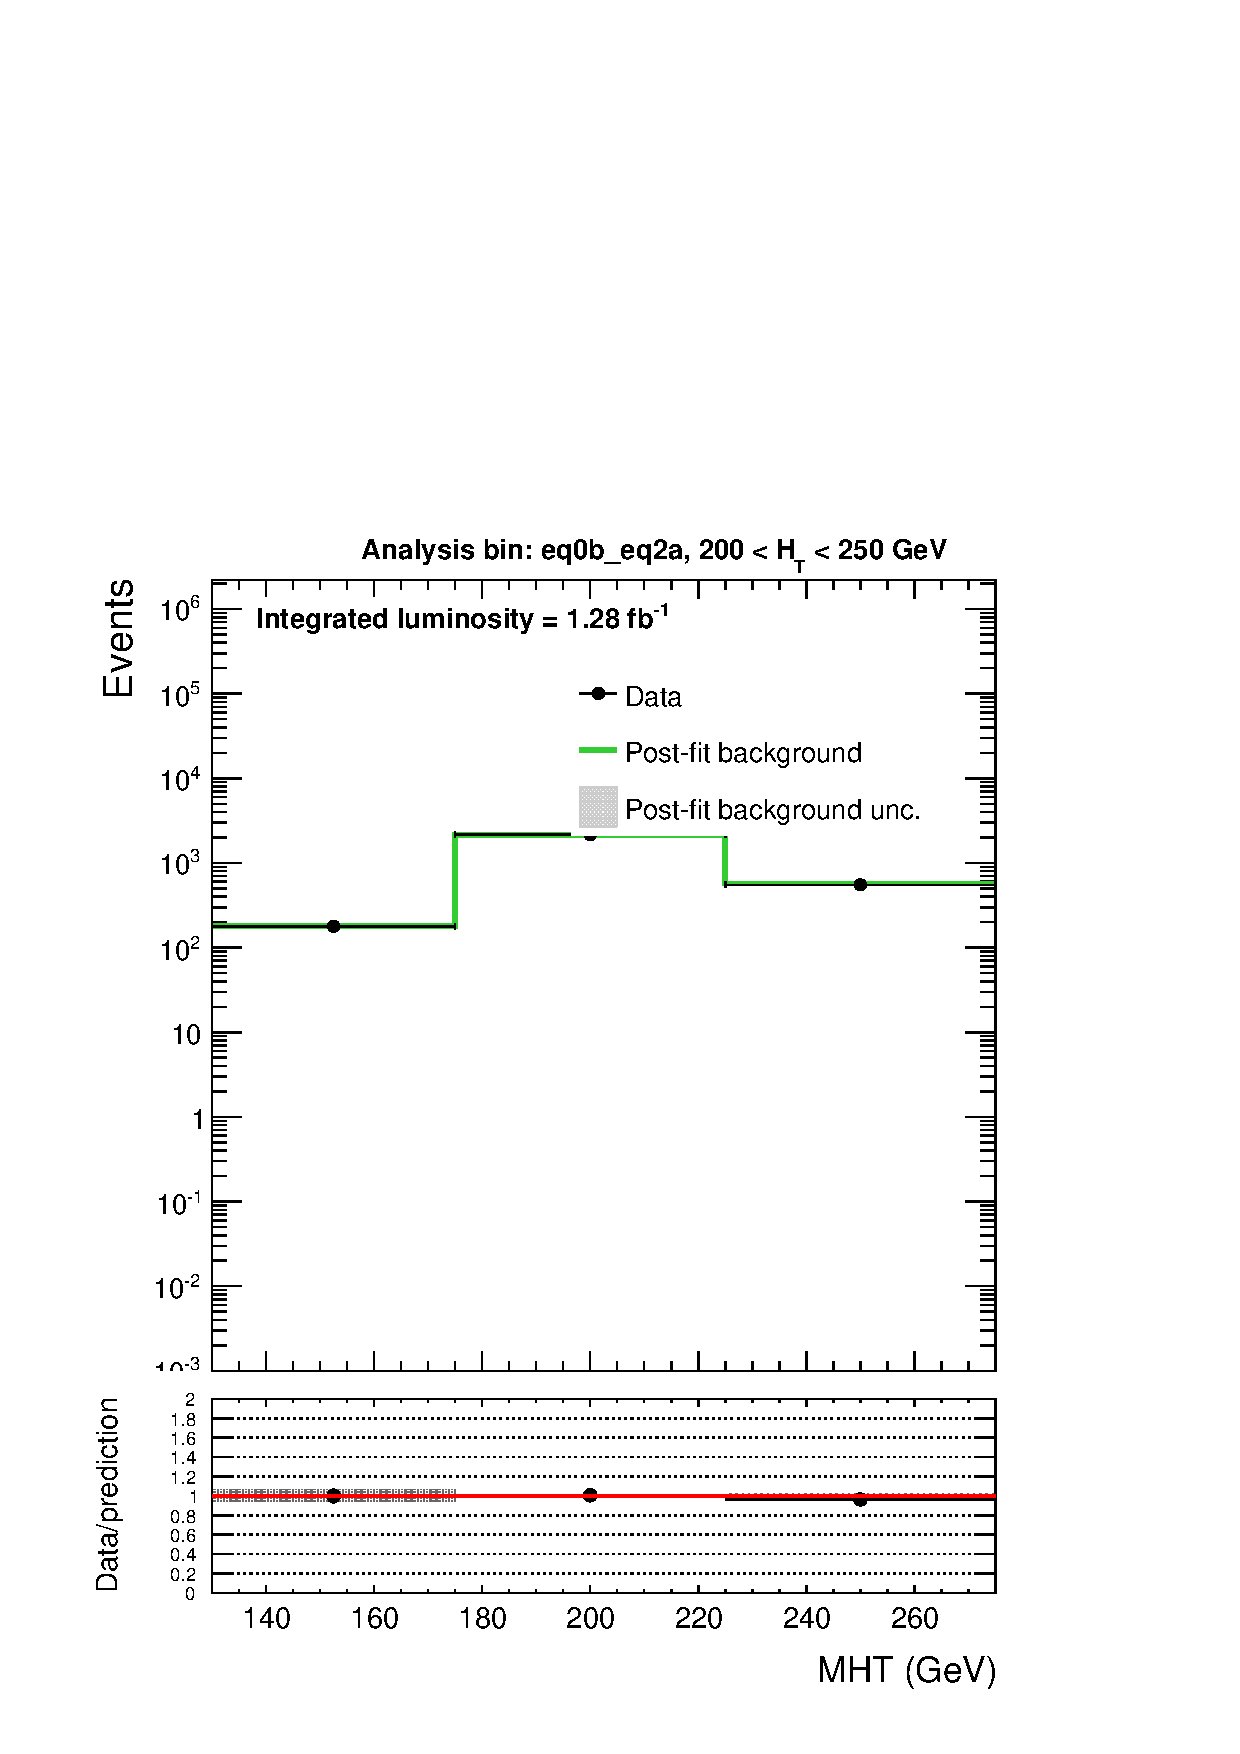
\includegraphics[width=0.25\textwidth]{figures/postFitResults/postFitShape_eq0b_eq2a_200_250.pdf} }\hspace{1cm}
    \subfigure[$\nj^{\mathrm{asym}}=2$, $\nb=0$, $250 < \scalht < 300 \; \mathrm{GeV}$]{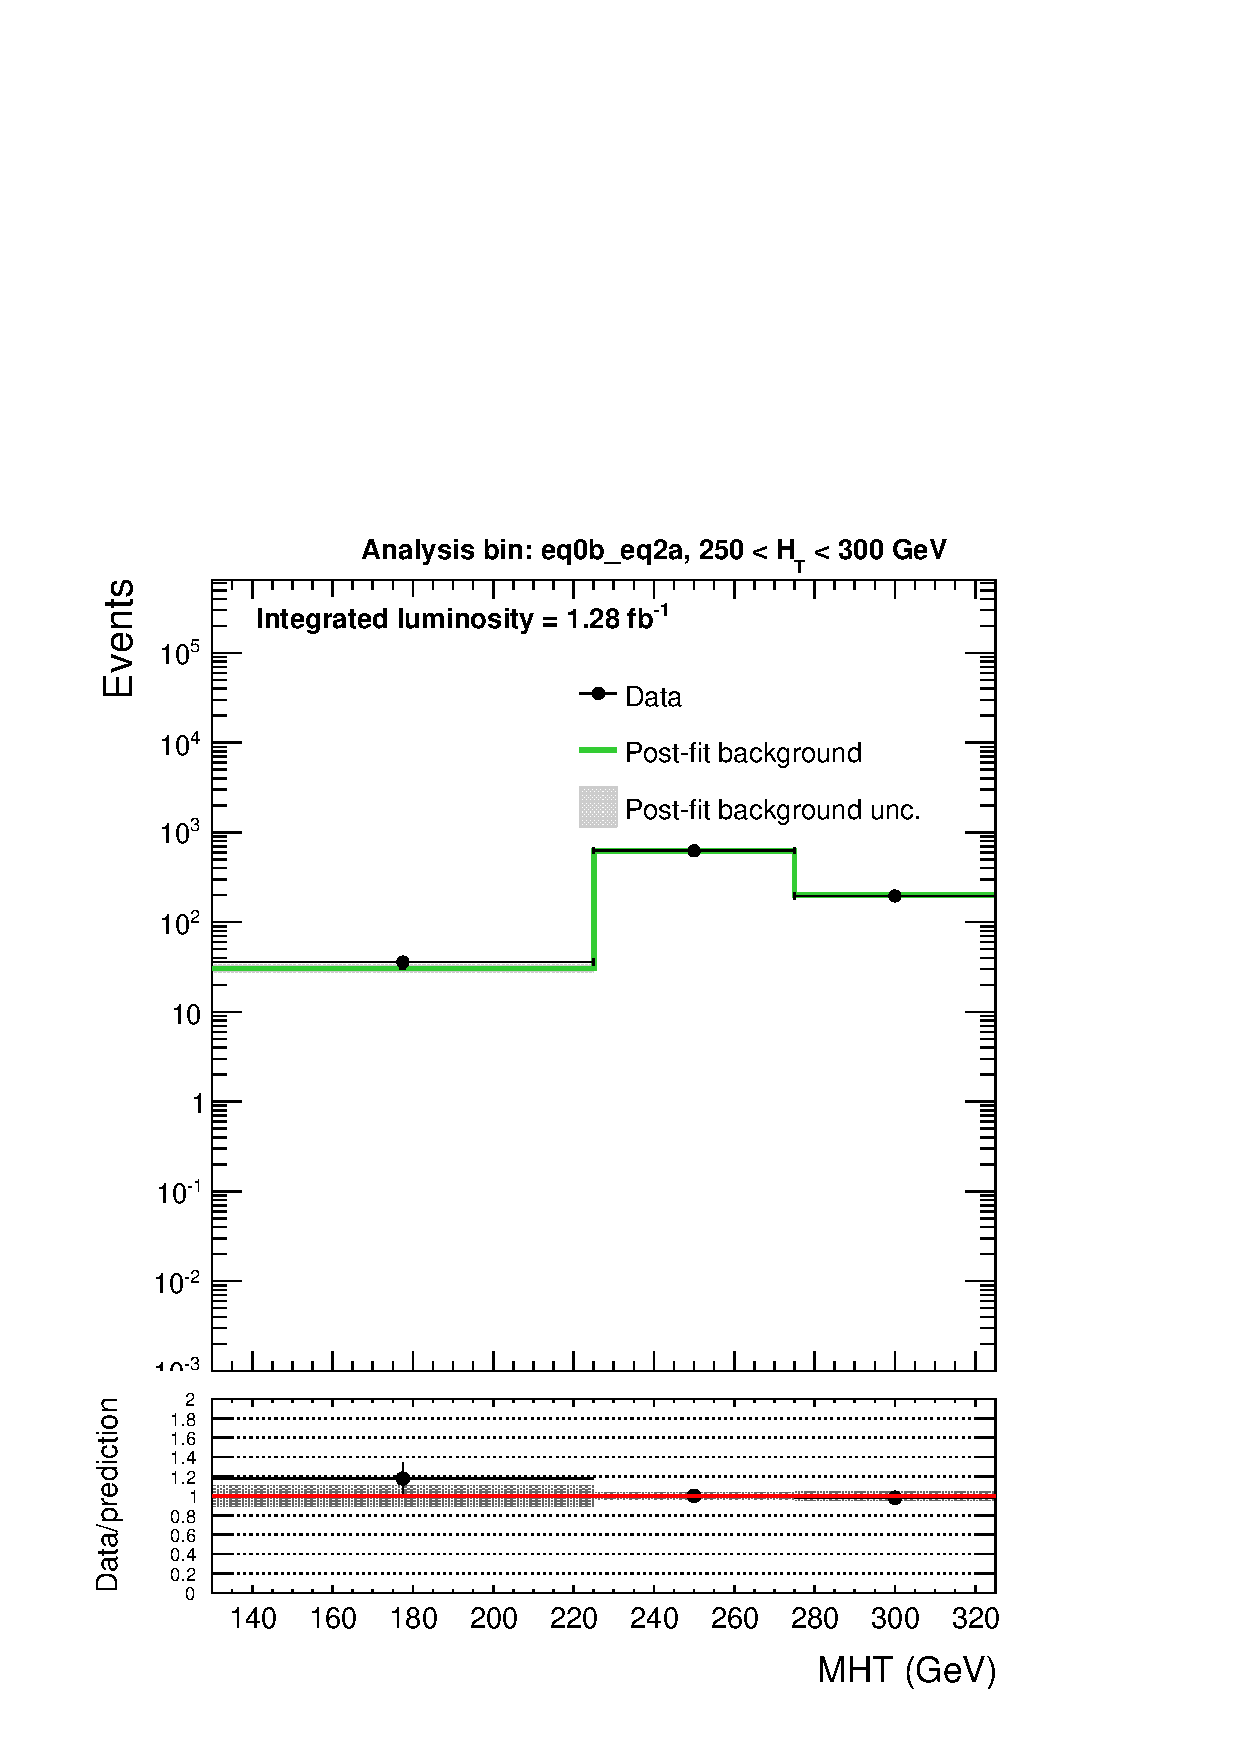
\includegraphics[width=0.25\textwidth]{figures/postFitResults/postFitShape_eq0b_eq2a_250_300.pdf} }\hspace{1cm}
    \subfigure[$\nj^{\mathrm{asym}}=2$, $\nb=0$, $300 < \scalht < 350 \; \mathrm{GeV}$]{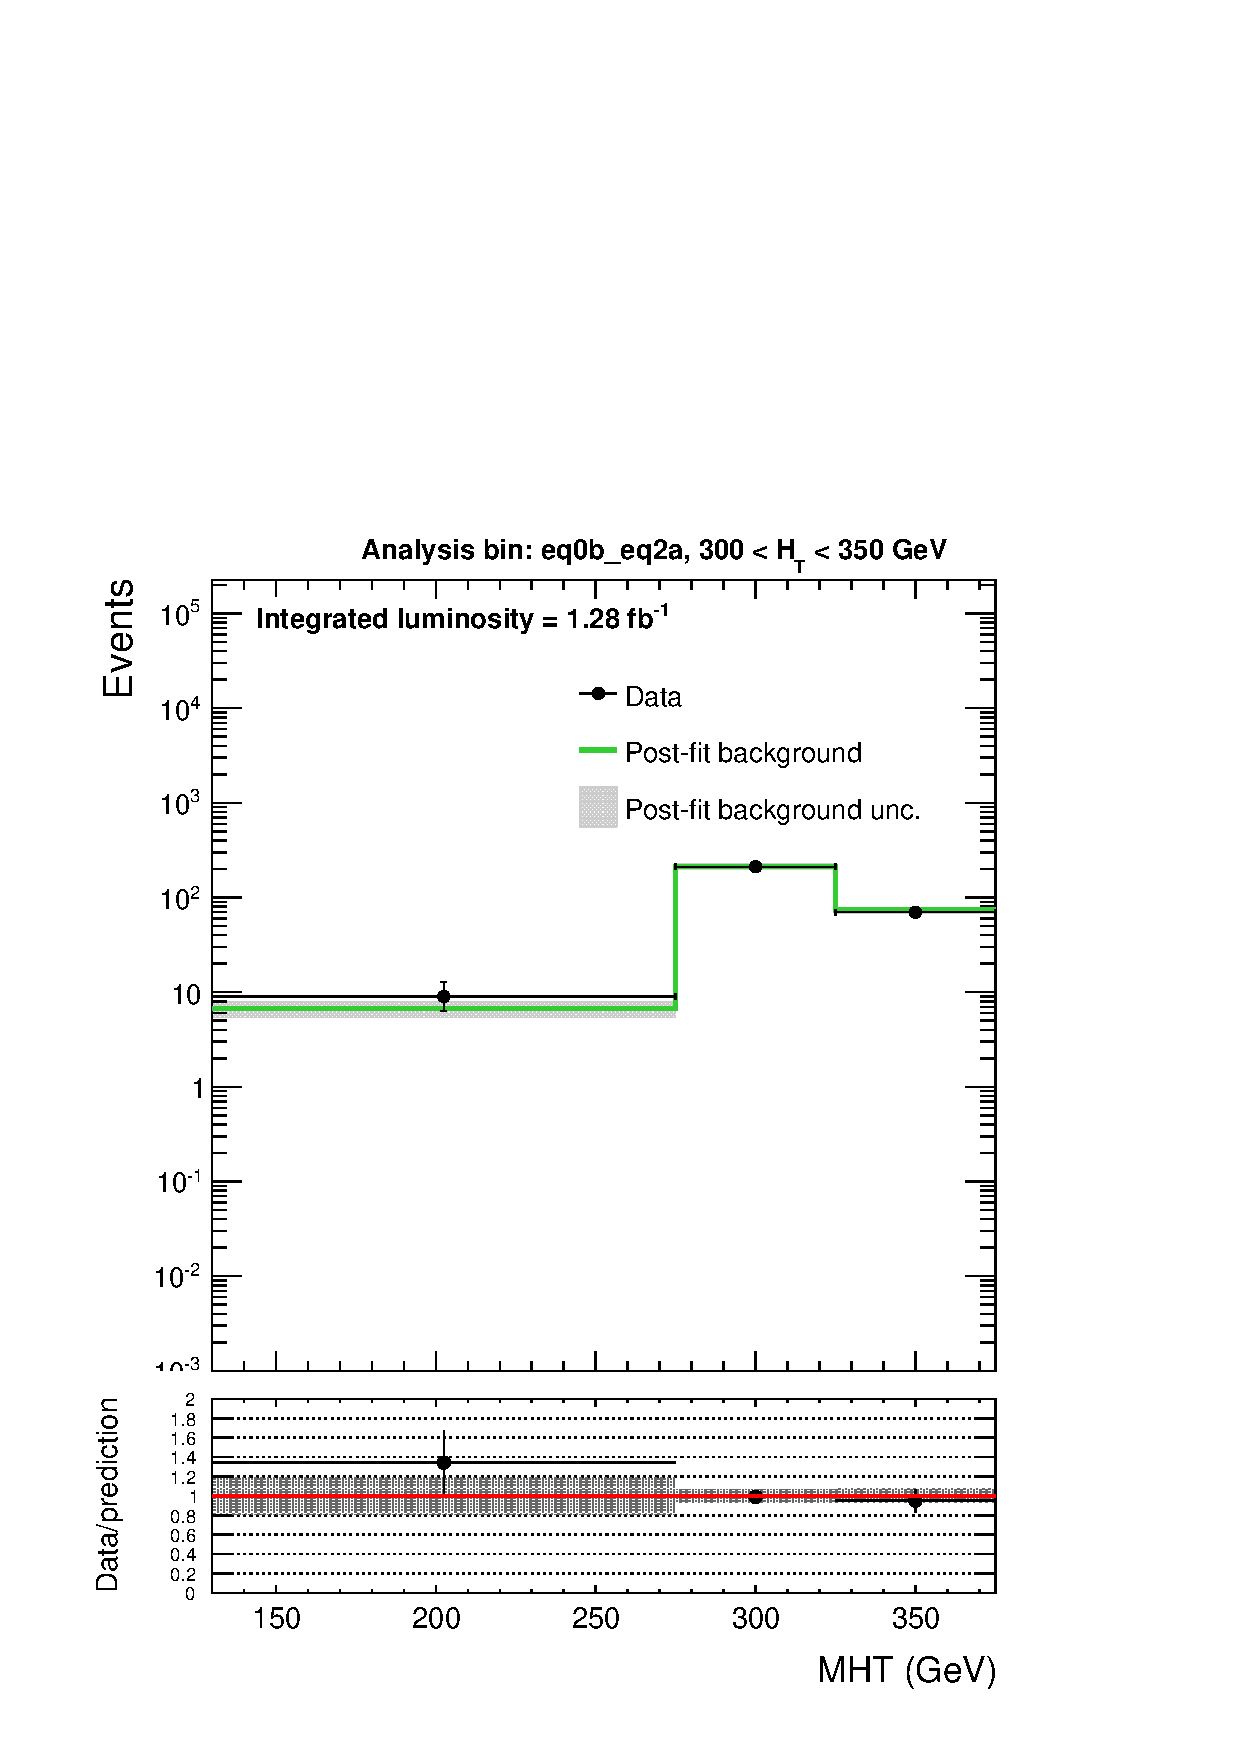
\includegraphics[width=0.25\textwidth]{figures/postFitResults/postFitShape_eq0b_eq2a_300_350.pdf} }\\
    \subfigure[$\nj^{\mathrm{asym}}=2$, $\nb=0$, $350 < \scalht < 400 \; \mathrm{GeV}$]{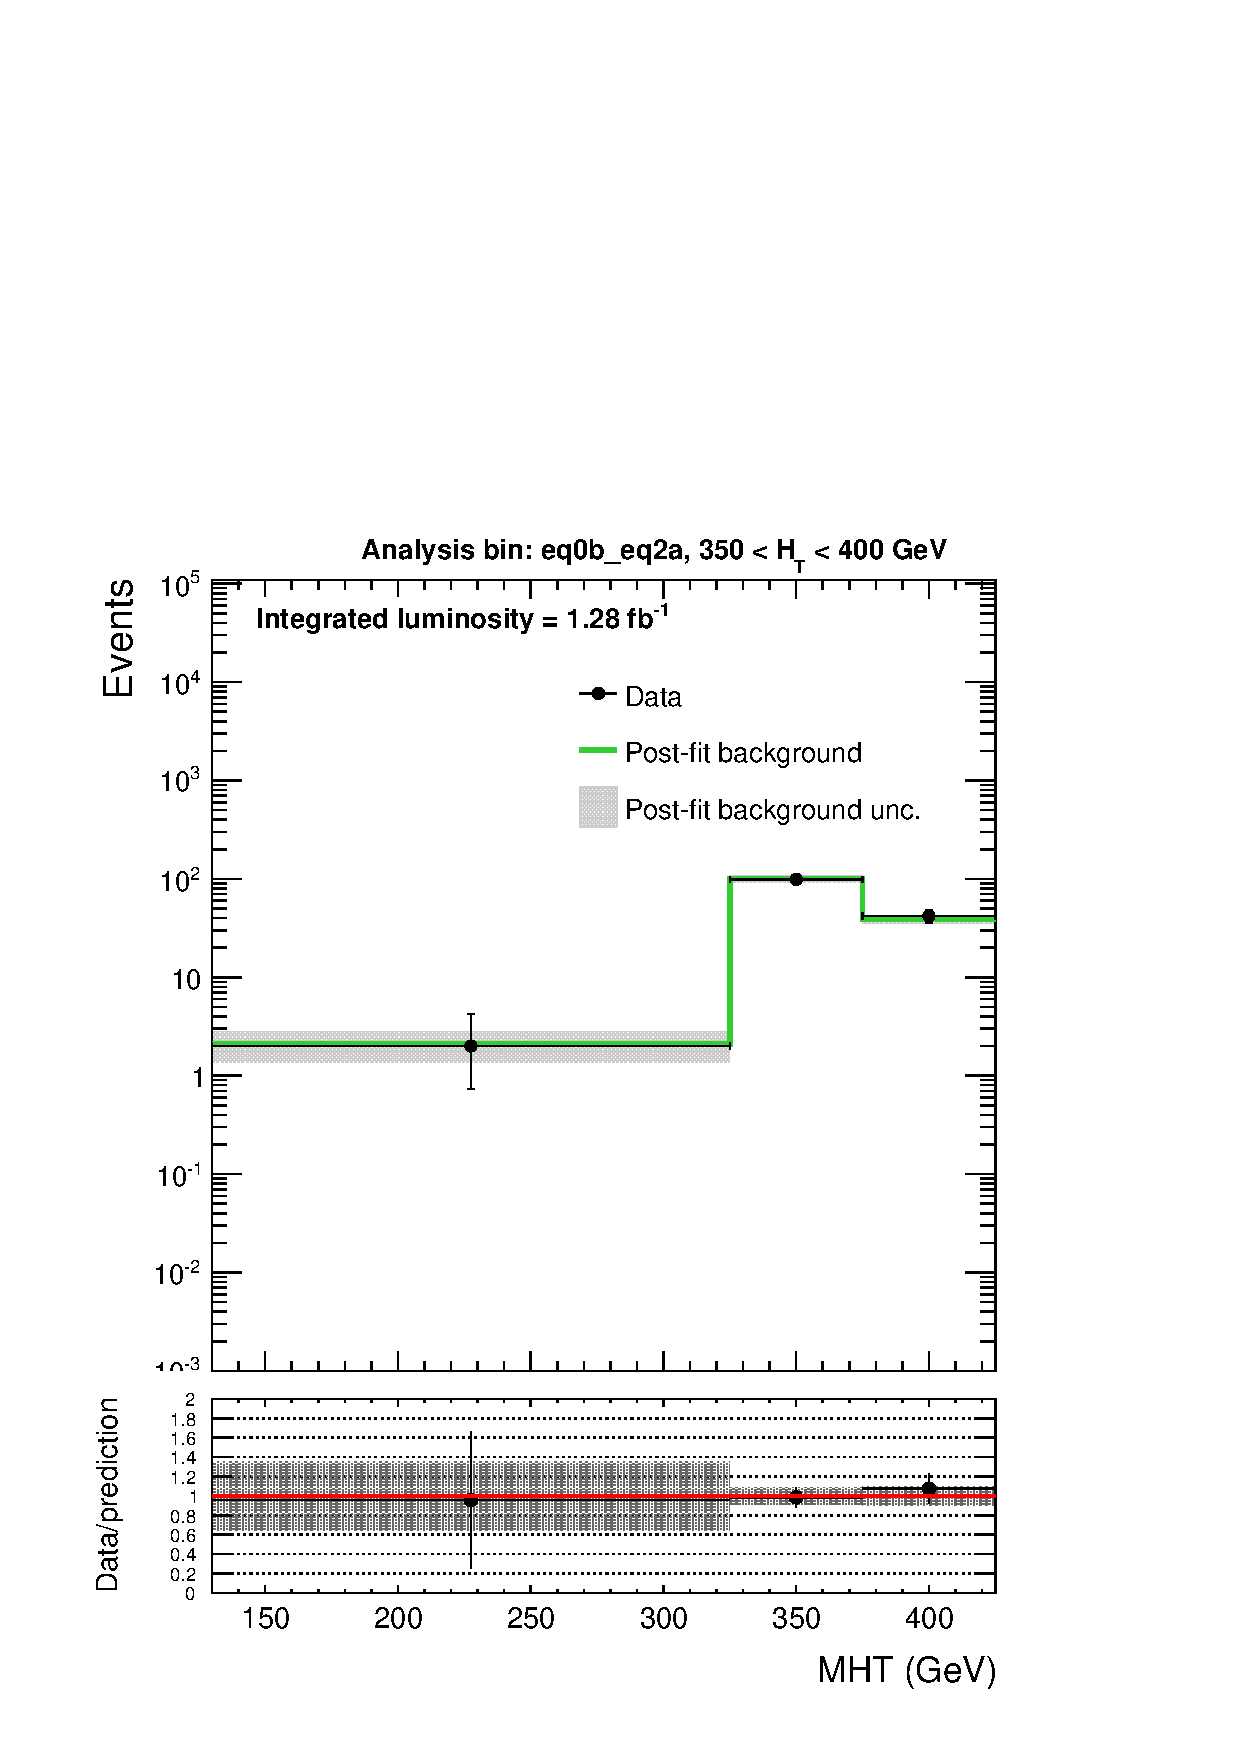
\includegraphics[width=0.25\textwidth]{figures/postFitResults/postFitShape_eq0b_eq2a_350_400.pdf} }\hspace{1cm}
    \subfigure[$\nj^{\mathrm{asym}}=2$, $\nb=0$, $400 < \scalht < 500 \; \mathrm{GeV}$]{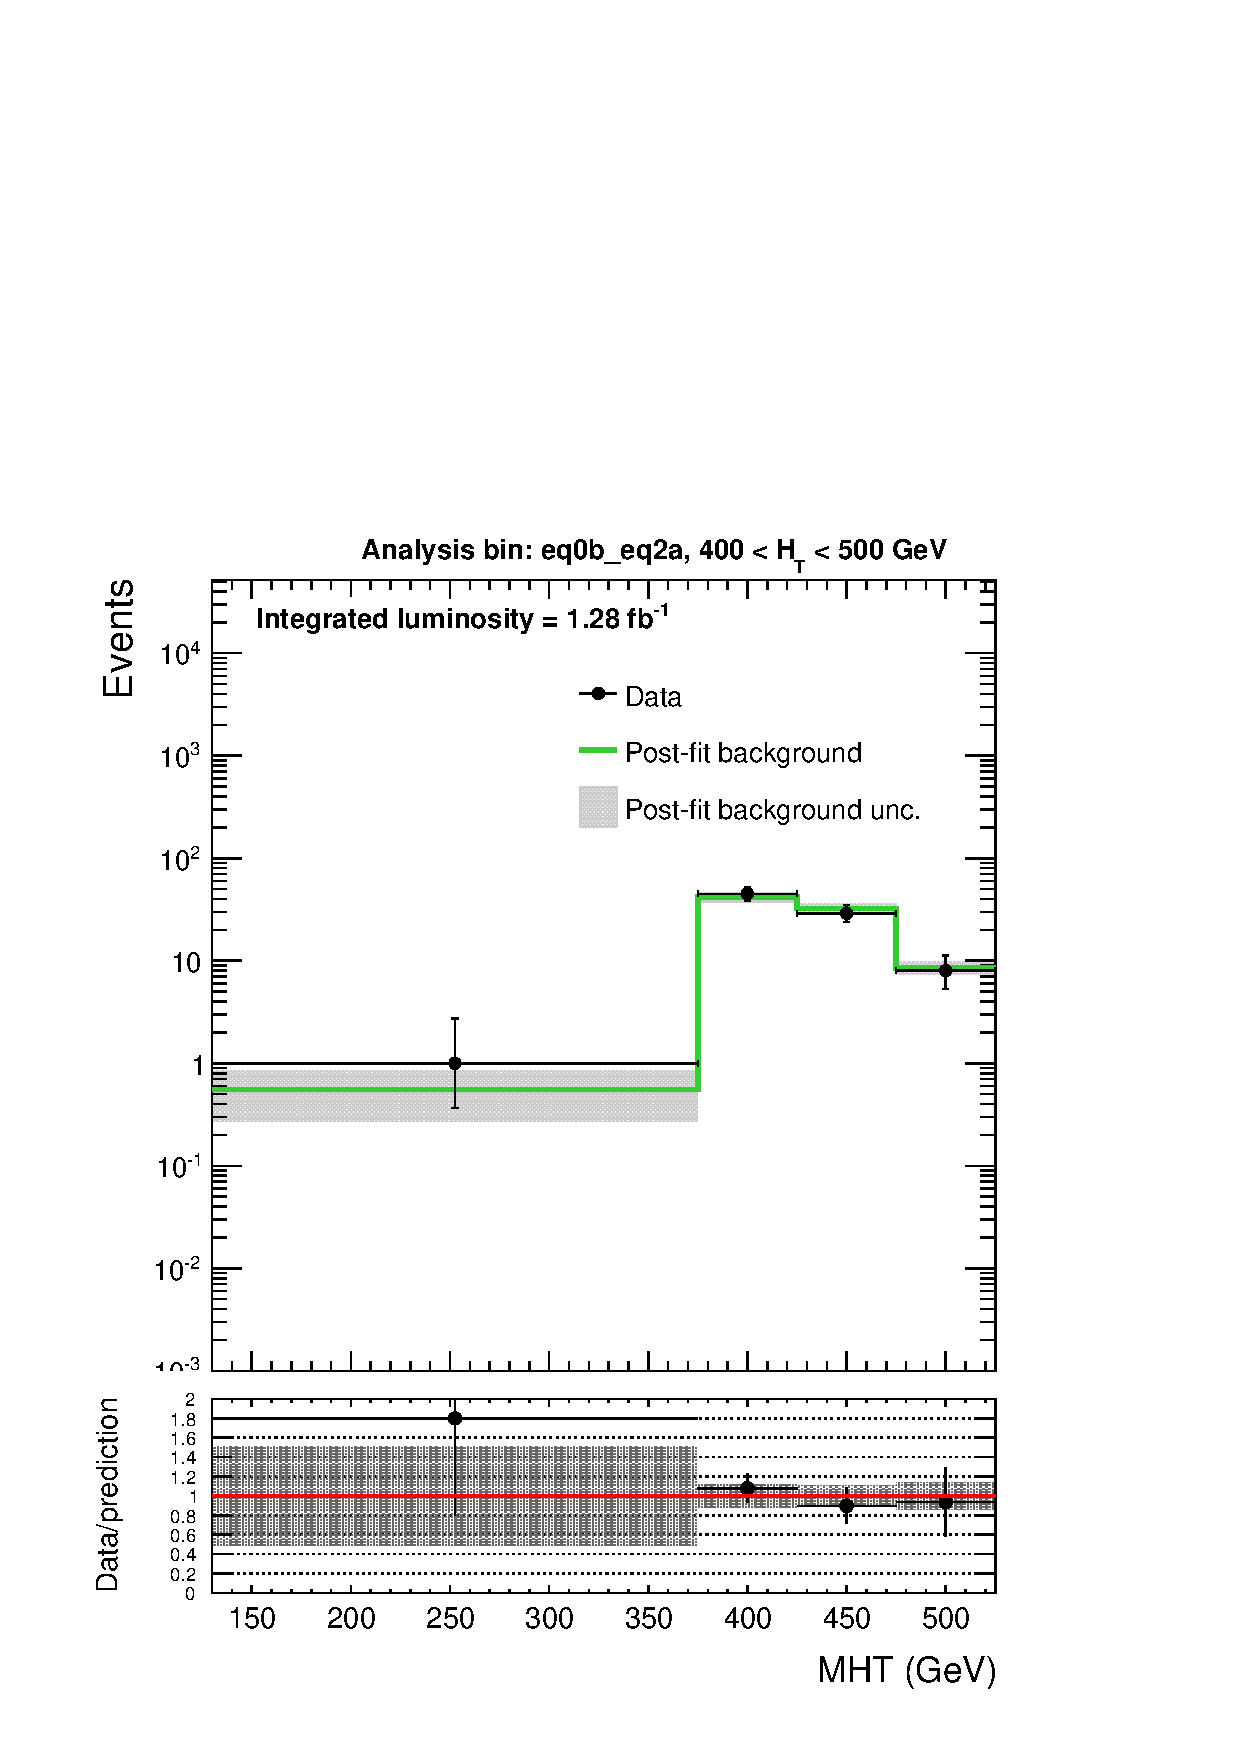
\includegraphics[width=0.25\textwidth]{figures/postFitResults/postFitShape_eq0b_eq2a_400_500.pdf} }\hspace{1cm}
    \subfigure[$\nj^{\mathrm{asym}}=2$, $\nb=0$, $500 < \scalht < 600 \; \mathrm{GeV}$]{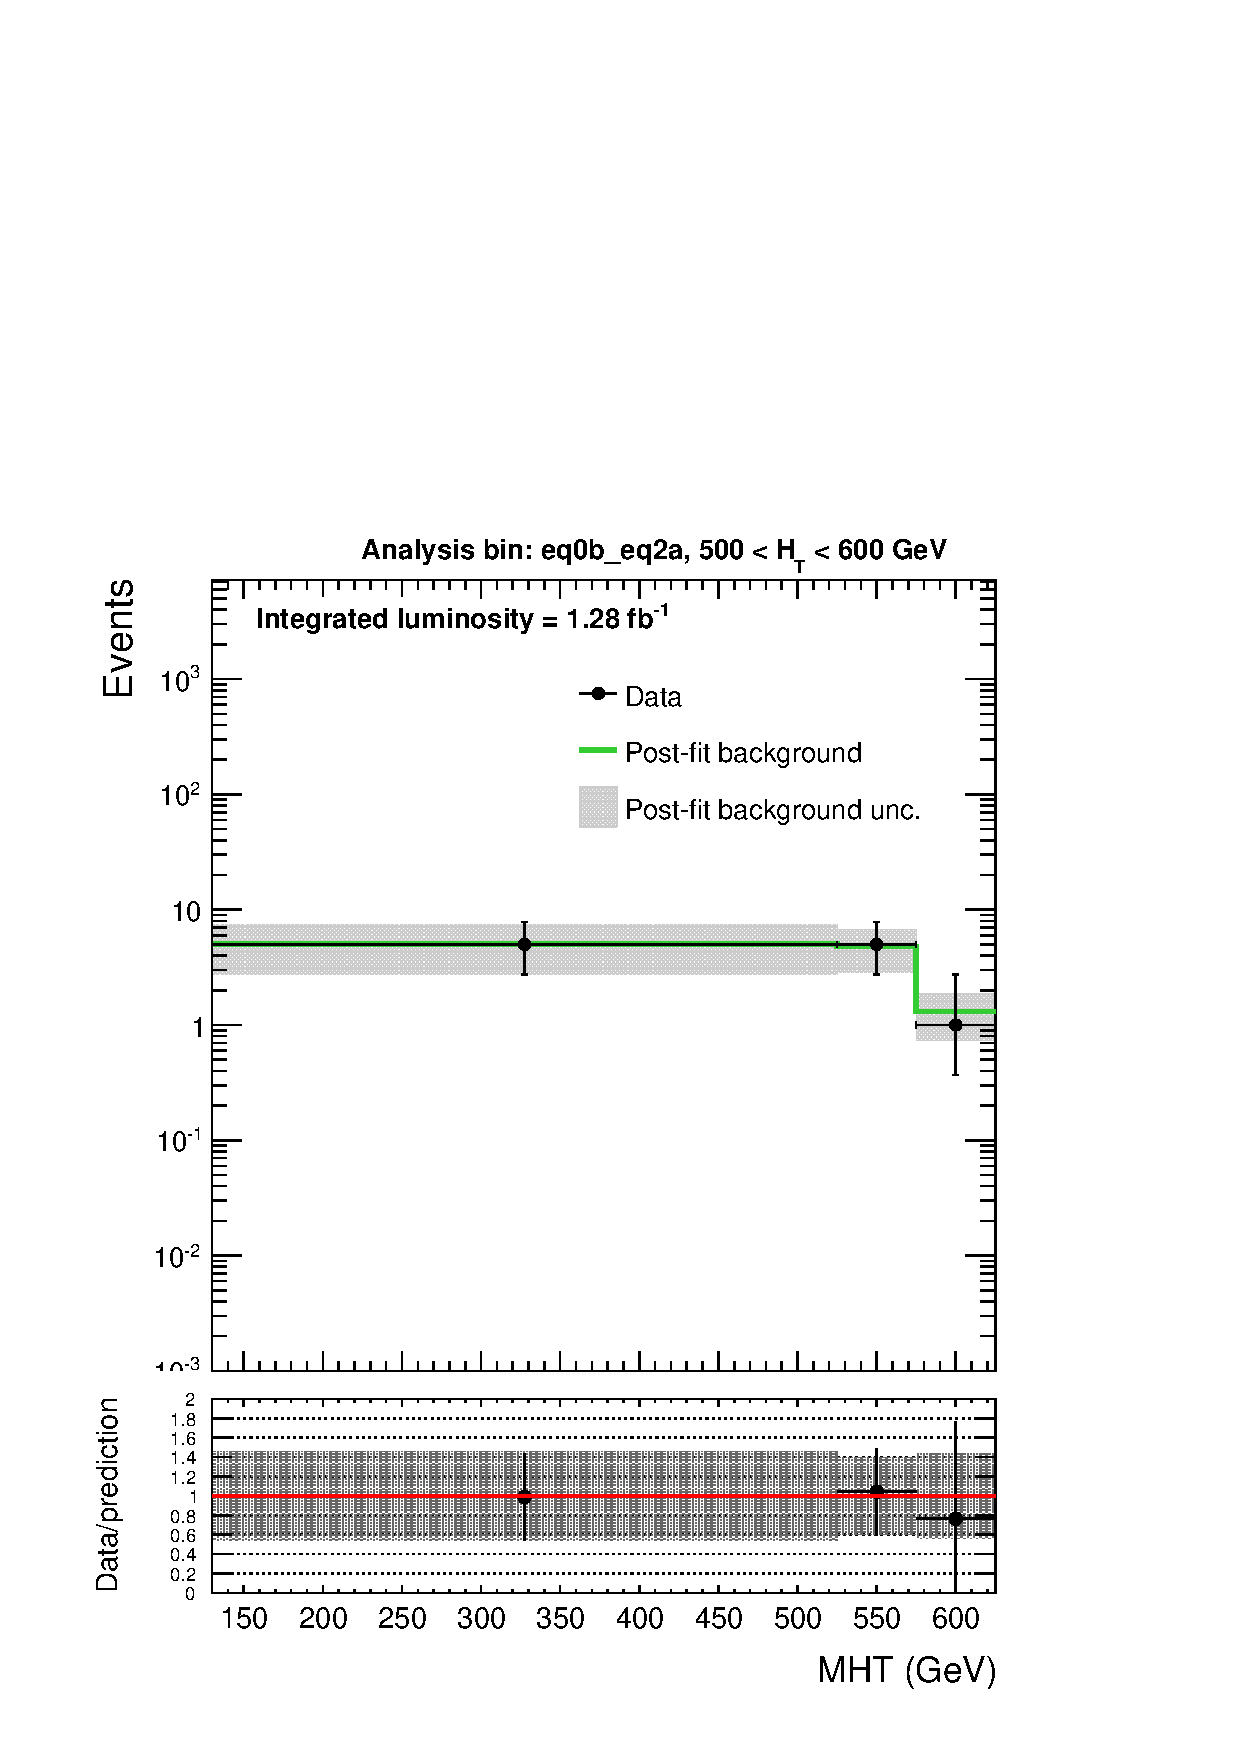
\includegraphics[width=0.25\textwidth]{figures/postFitResults/postFitShape_eq0b_eq2a_500_600.pdf} }\\
    \subfigure[$\nj^{\mathrm{asym}}=2$, $\nb=0$, $\scalht > 600 \; \mathrm{GeV}$]{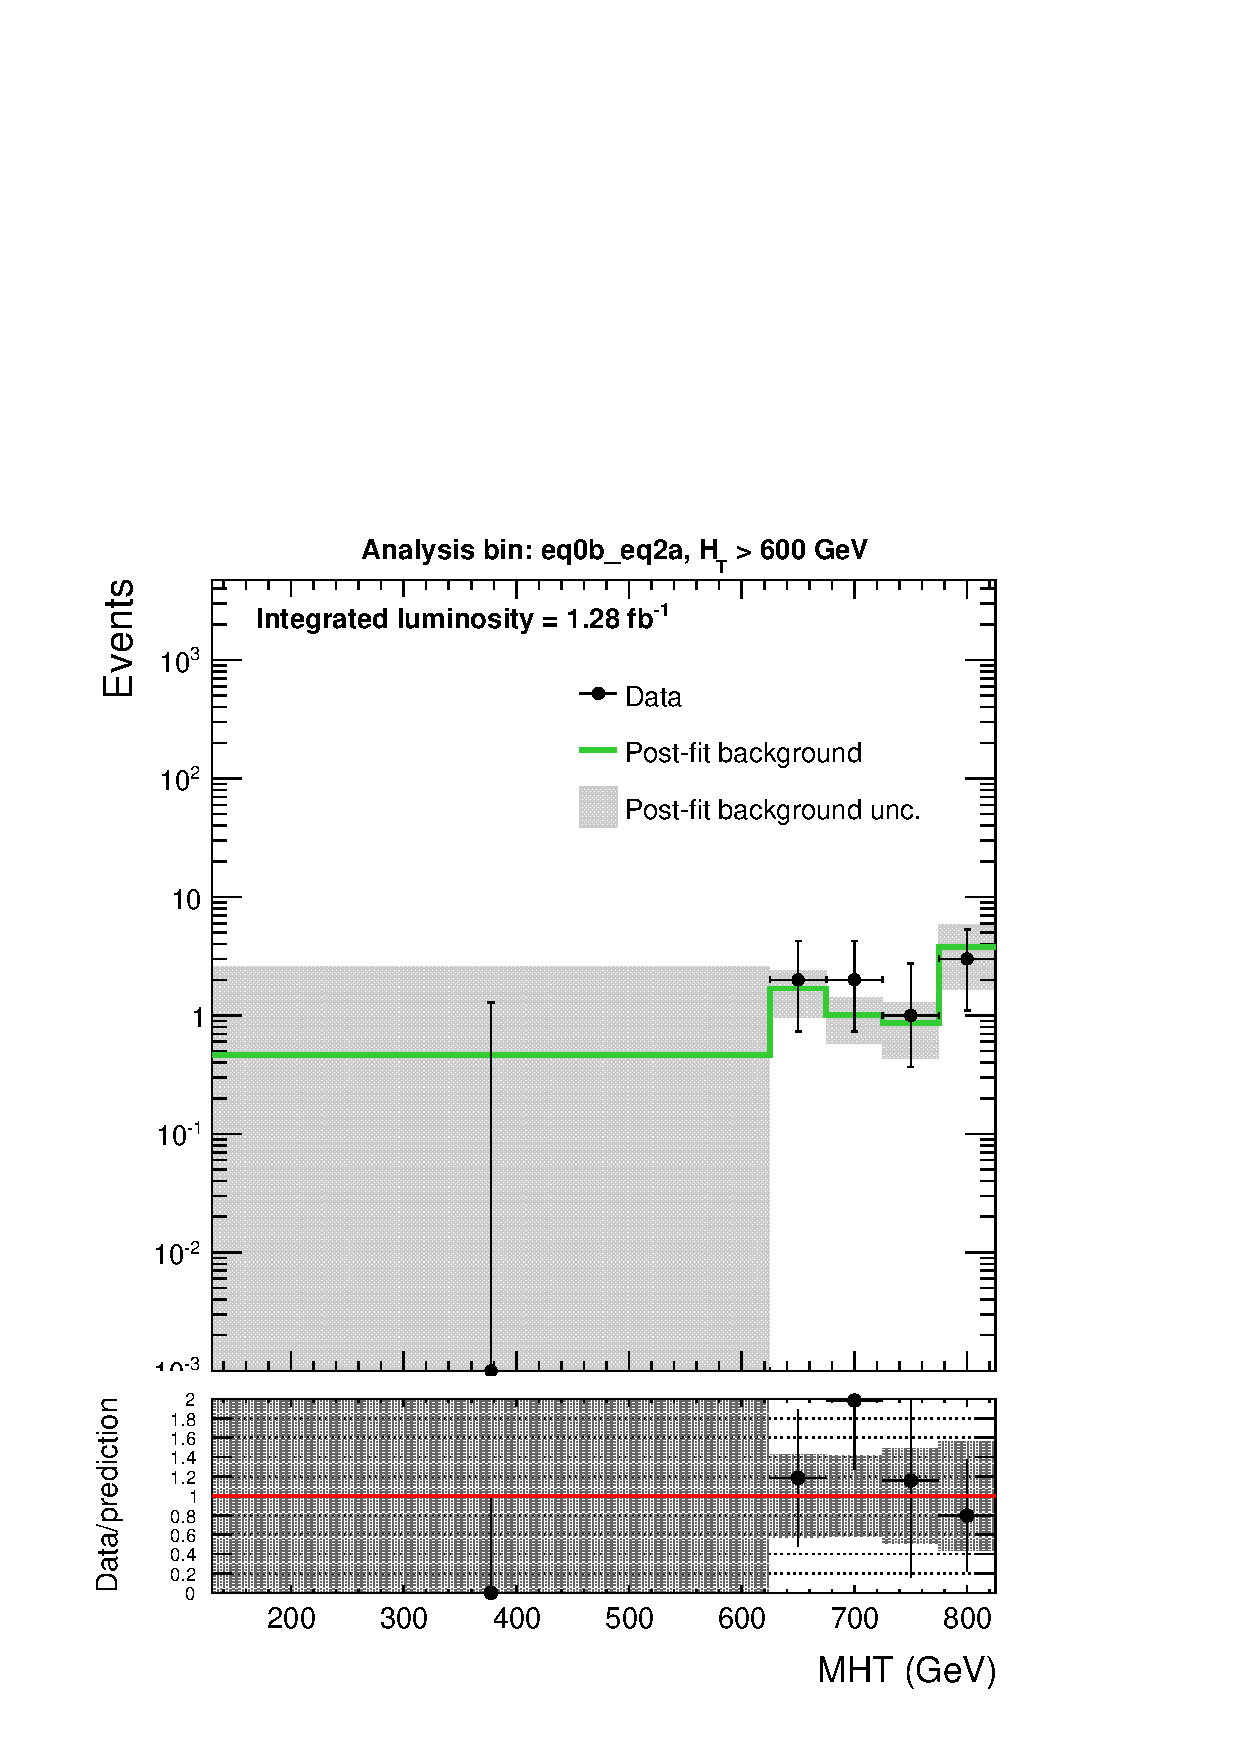
\includegraphics[width=0.25\textwidth]{figures/postFitResults/postFitShape_eq0b_eq2a_600_Inf.pdf} }\hspace{1cm}
  \end{center}
\end{figure}



\newpage
\begin{figure}[h!]
\caption{Post-fit \MHT templates for the bin $\nj^{\mathrm{sym}}=2$, $\nb=0$ \label{fig:postFitShapes_eq0b_eq2j}}.
\begin{center}

    \subfigure[$\nj^{\mathrm{sym}}=2$, $\nb=0$, $200 < \scalht < 250 \; \mathrm{GeV}$]{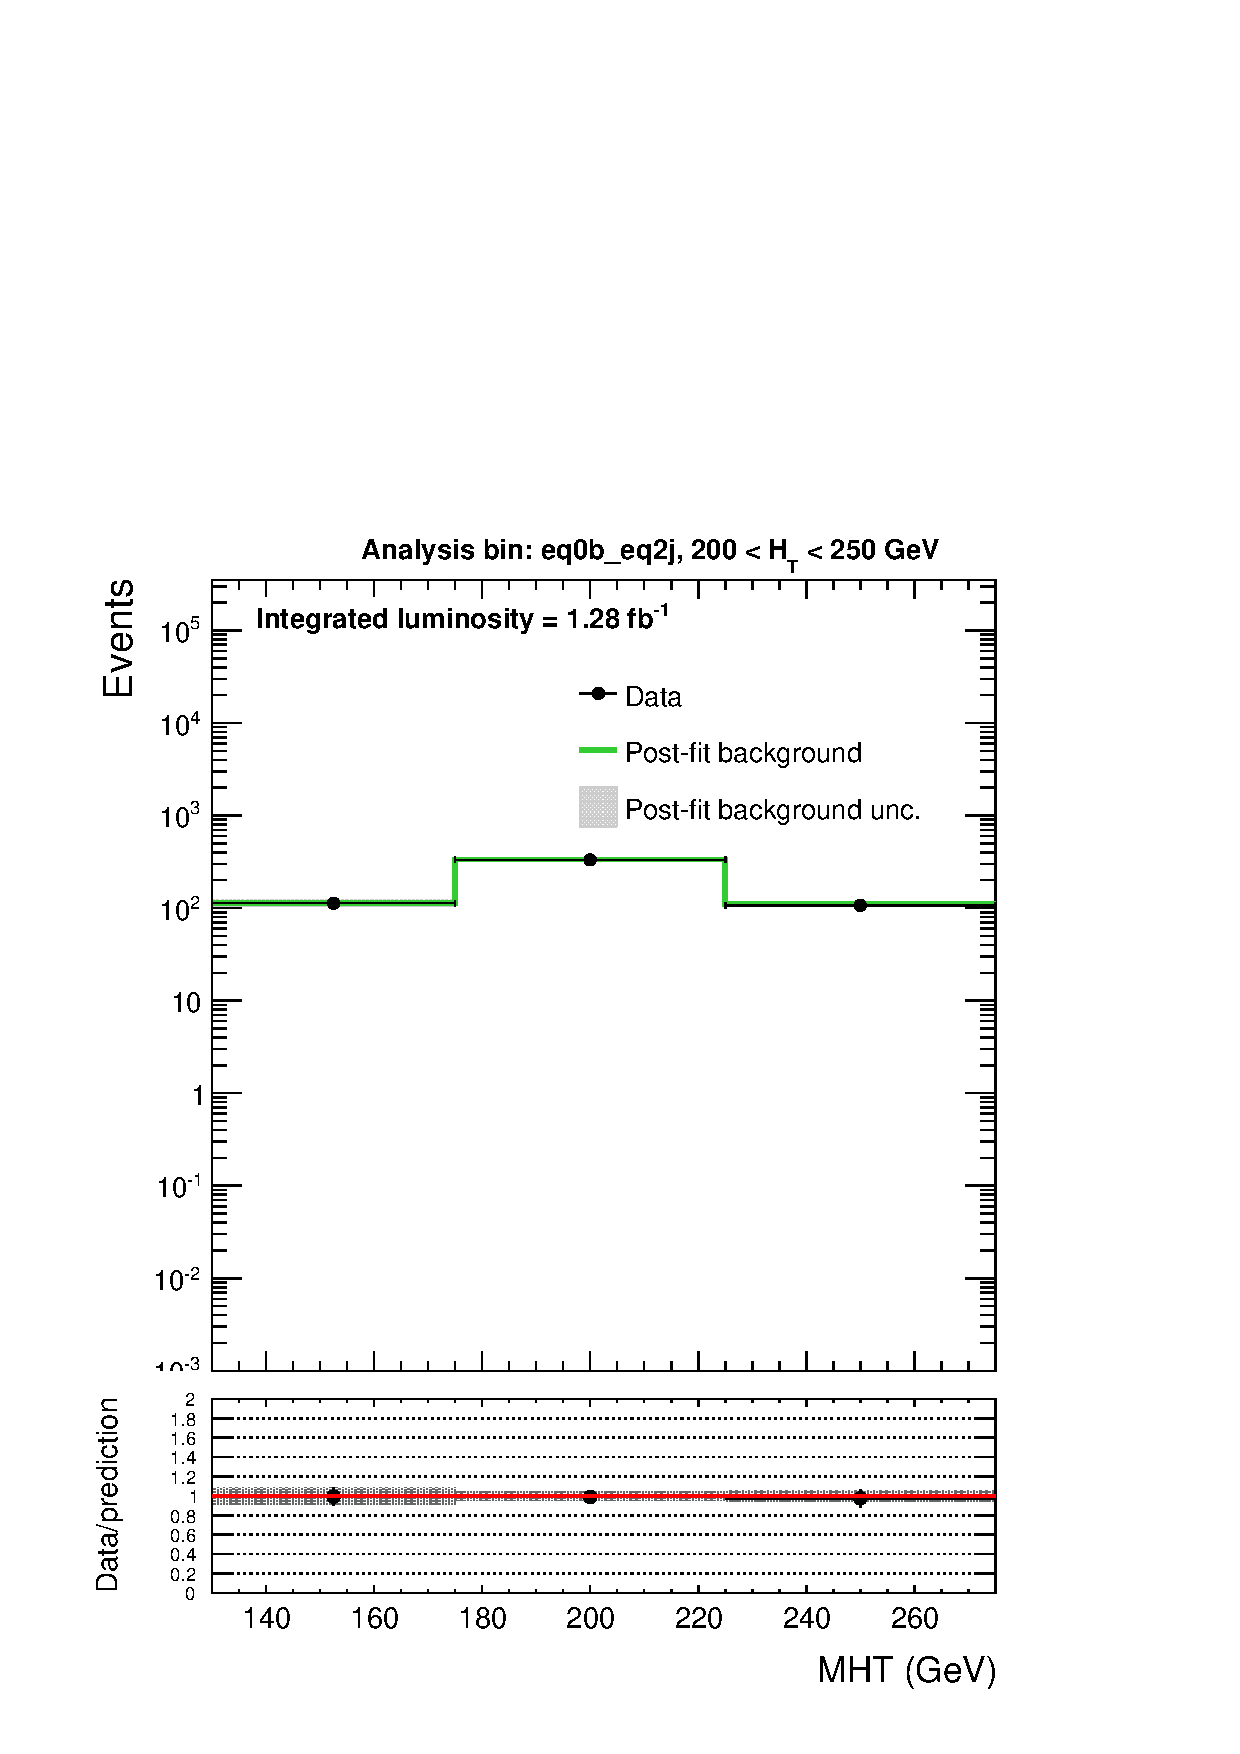
\includegraphics[width=0.25\textwidth]{figures/postFitResults/postFitShape_eq0b_eq2j_200_250.pdf} }\hspace{1cm}
    \subfigure[$\nj^{\mathrm{sym}}=2$, $\nb=0$, $250 < \scalht < 300 \; \mathrm{GeV}$]{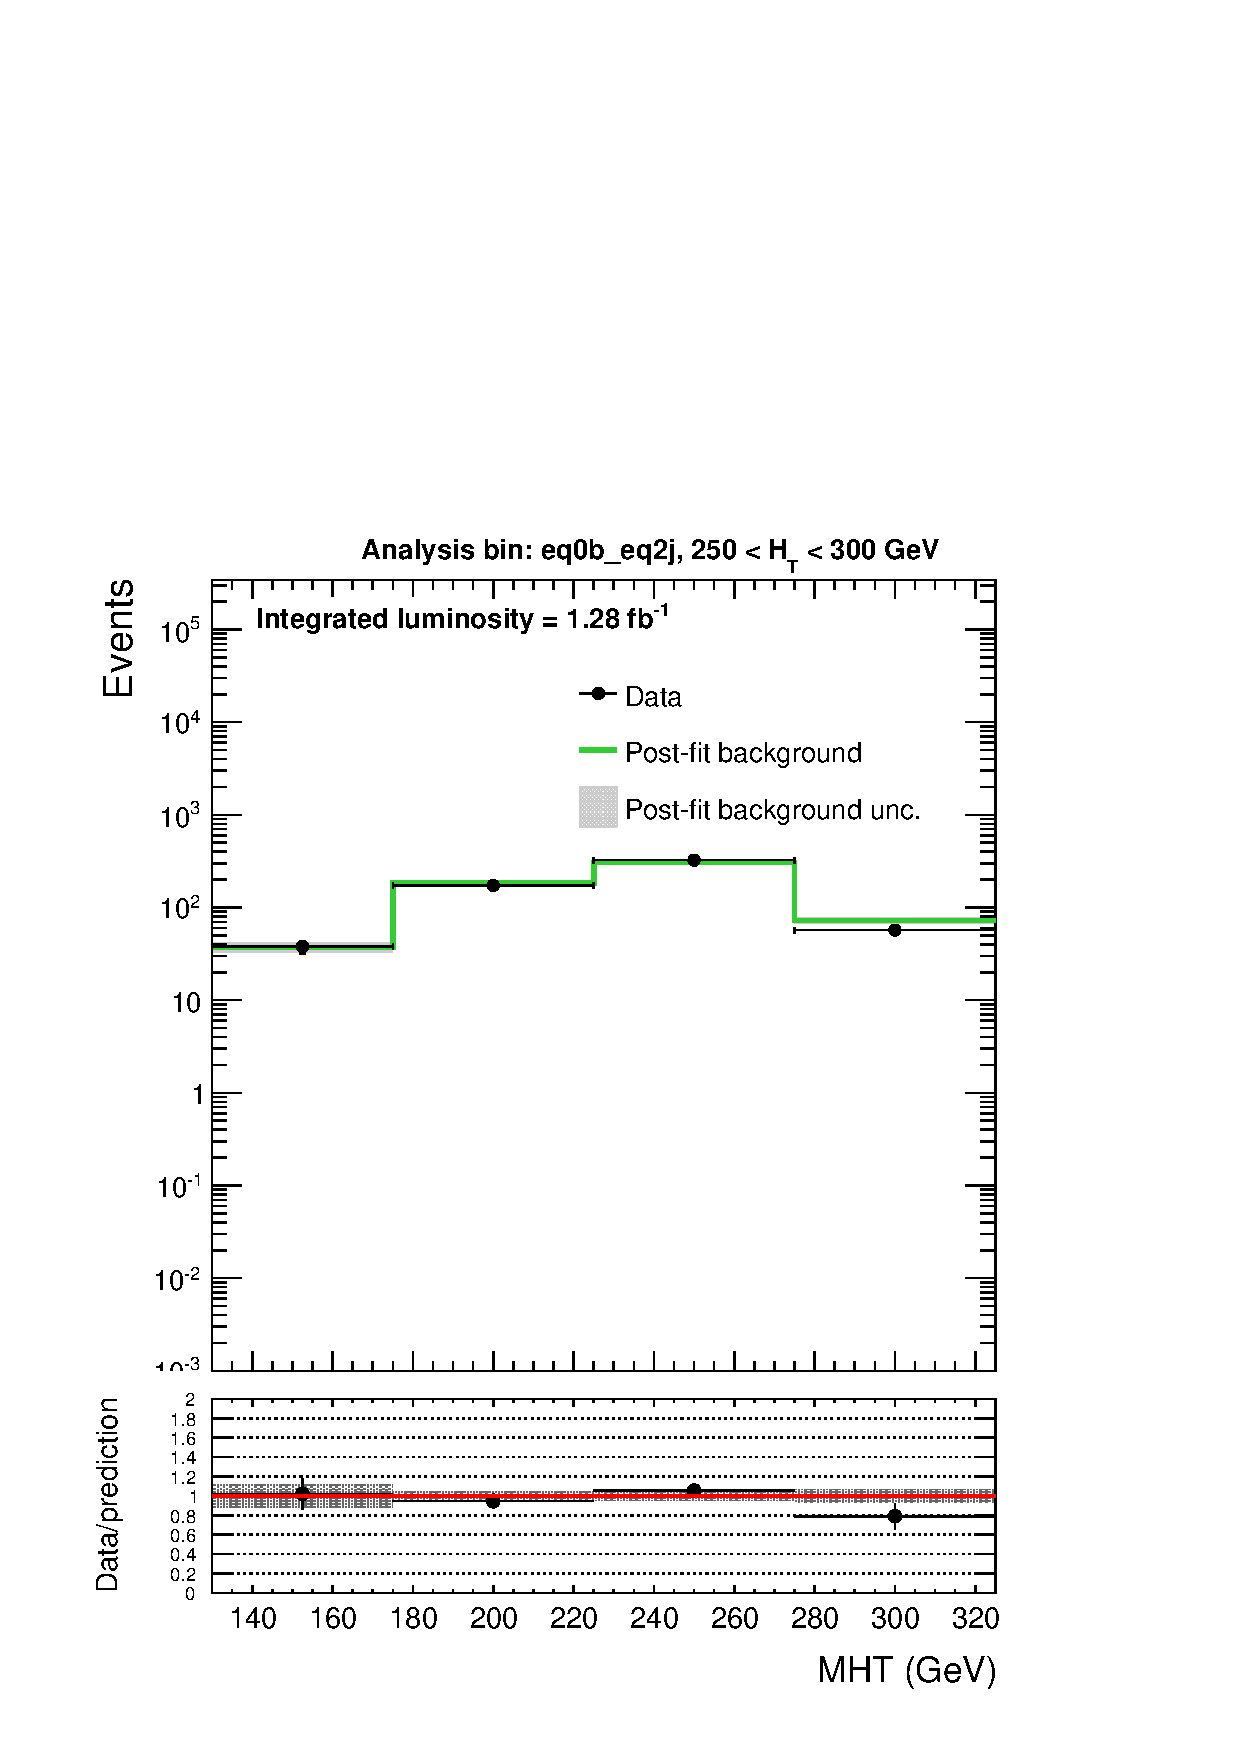
\includegraphics[width=0.25\textwidth]{figures/postFitResults/postFitShape_eq0b_eq2j_250_300.pdf} }\hspace{1cm}
    \subfigure[$\nj^{\mathrm{sym}}=2$, $\nb=0$, $300 < \scalht < 350 \; \mathrm{GeV}$]{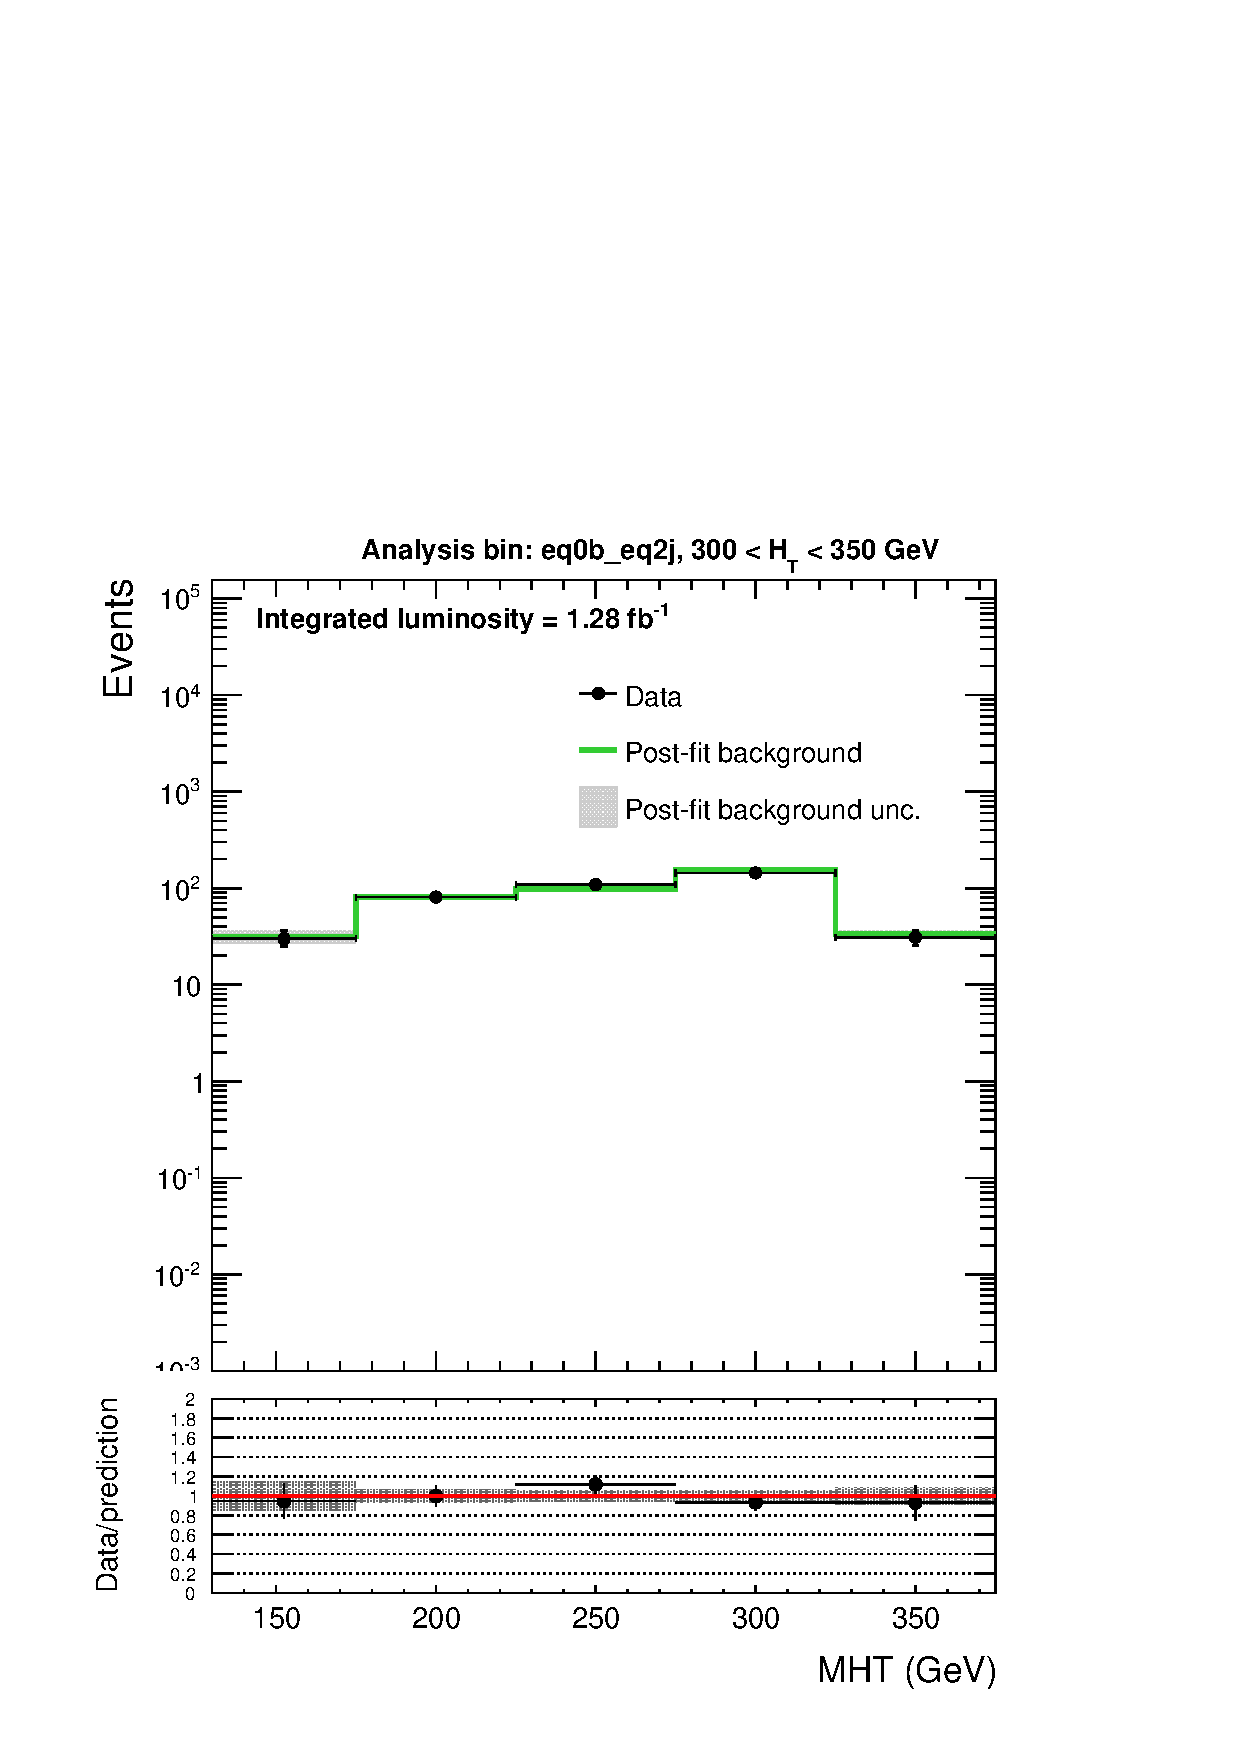
\includegraphics[width=0.25\textwidth]{figures/postFitResults/postFitShape_eq0b_eq2j_300_350.pdf} }\\
    \subfigure[$\nj^{\mathrm{sym}}=2$, $\nb=0$, $350 < \scalht < 400 \; \mathrm{GeV}$]{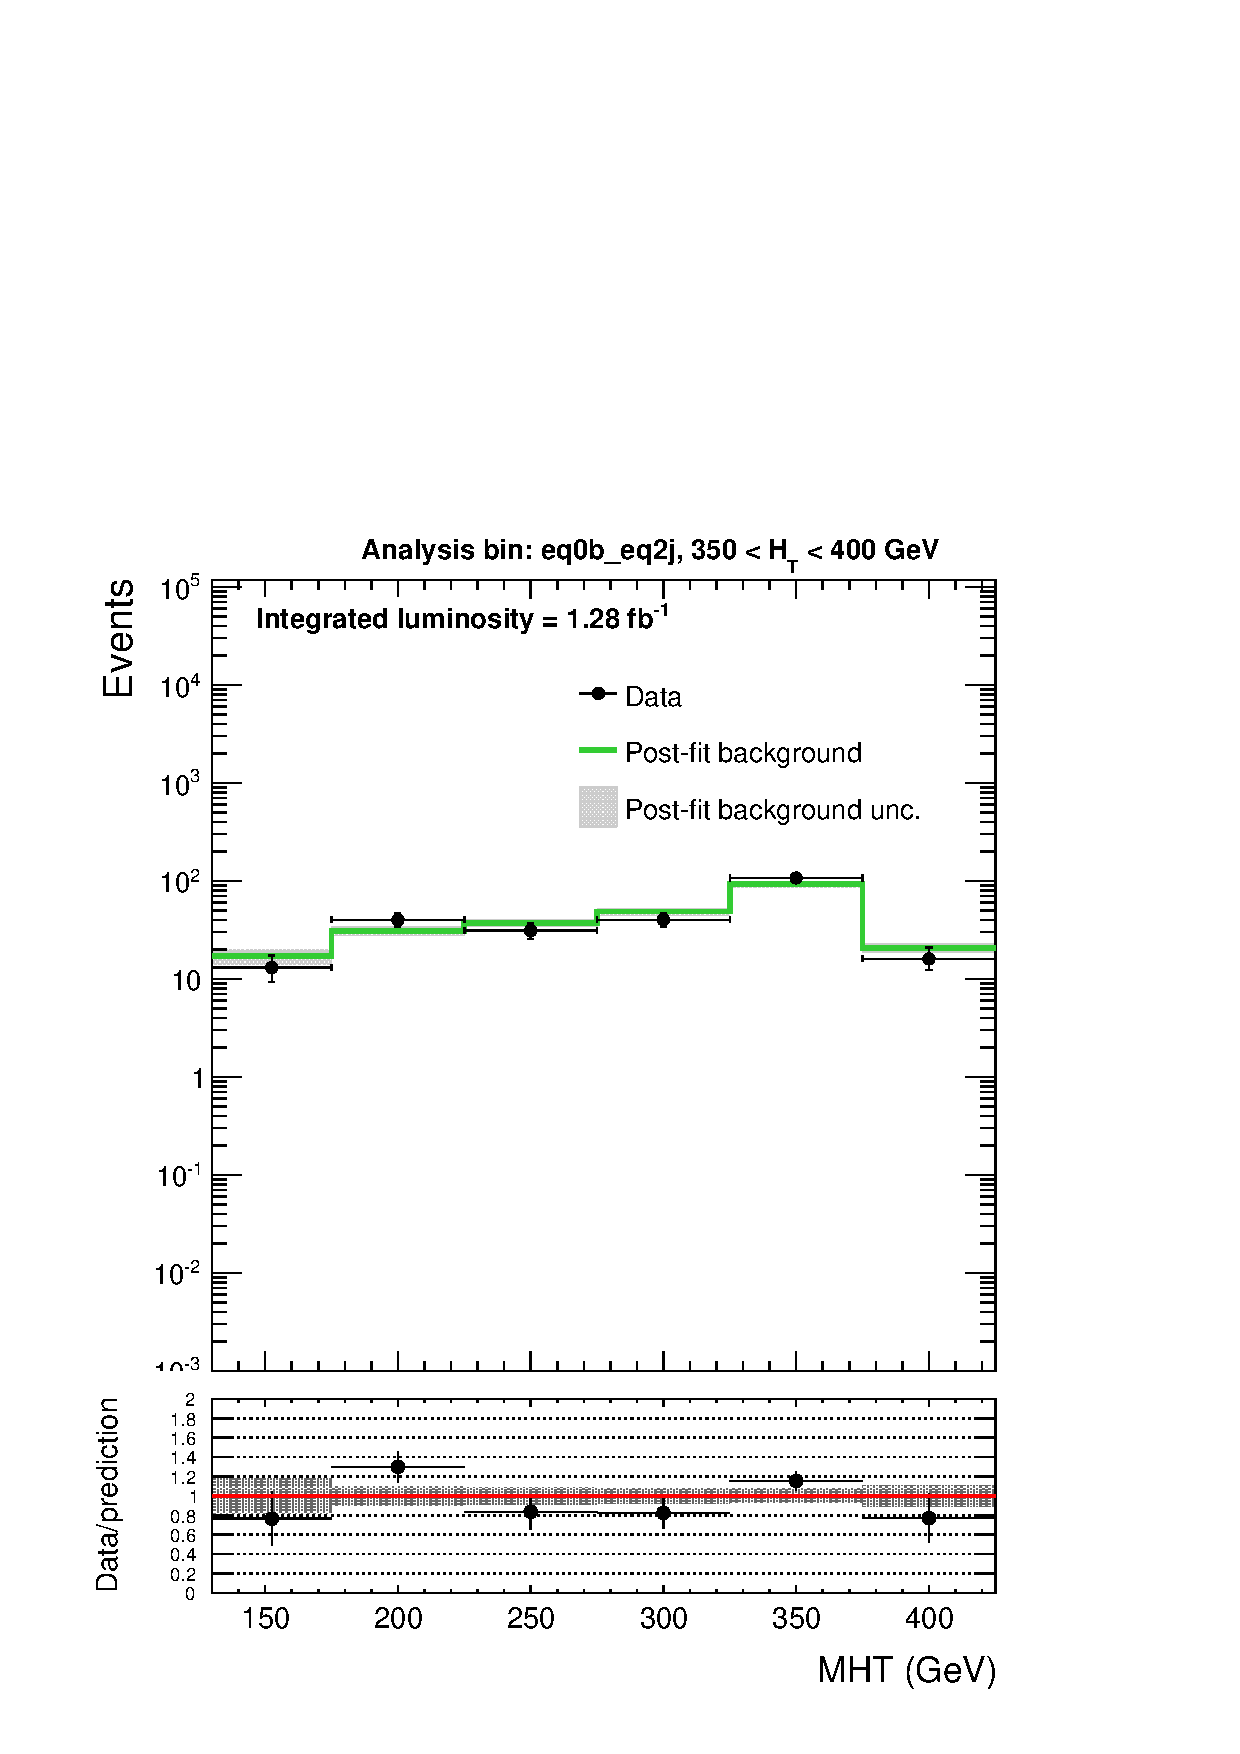
\includegraphics[width=0.25\textwidth]{figures/postFitResults/postFitShape_eq0b_eq2j_350_400.pdf} }\hspace{1cm}
    \subfigure[$\nj^{\mathrm{sym}}=2$, $\nb=0$, $400 < \scalht < 500 \; \mathrm{GeV}$]{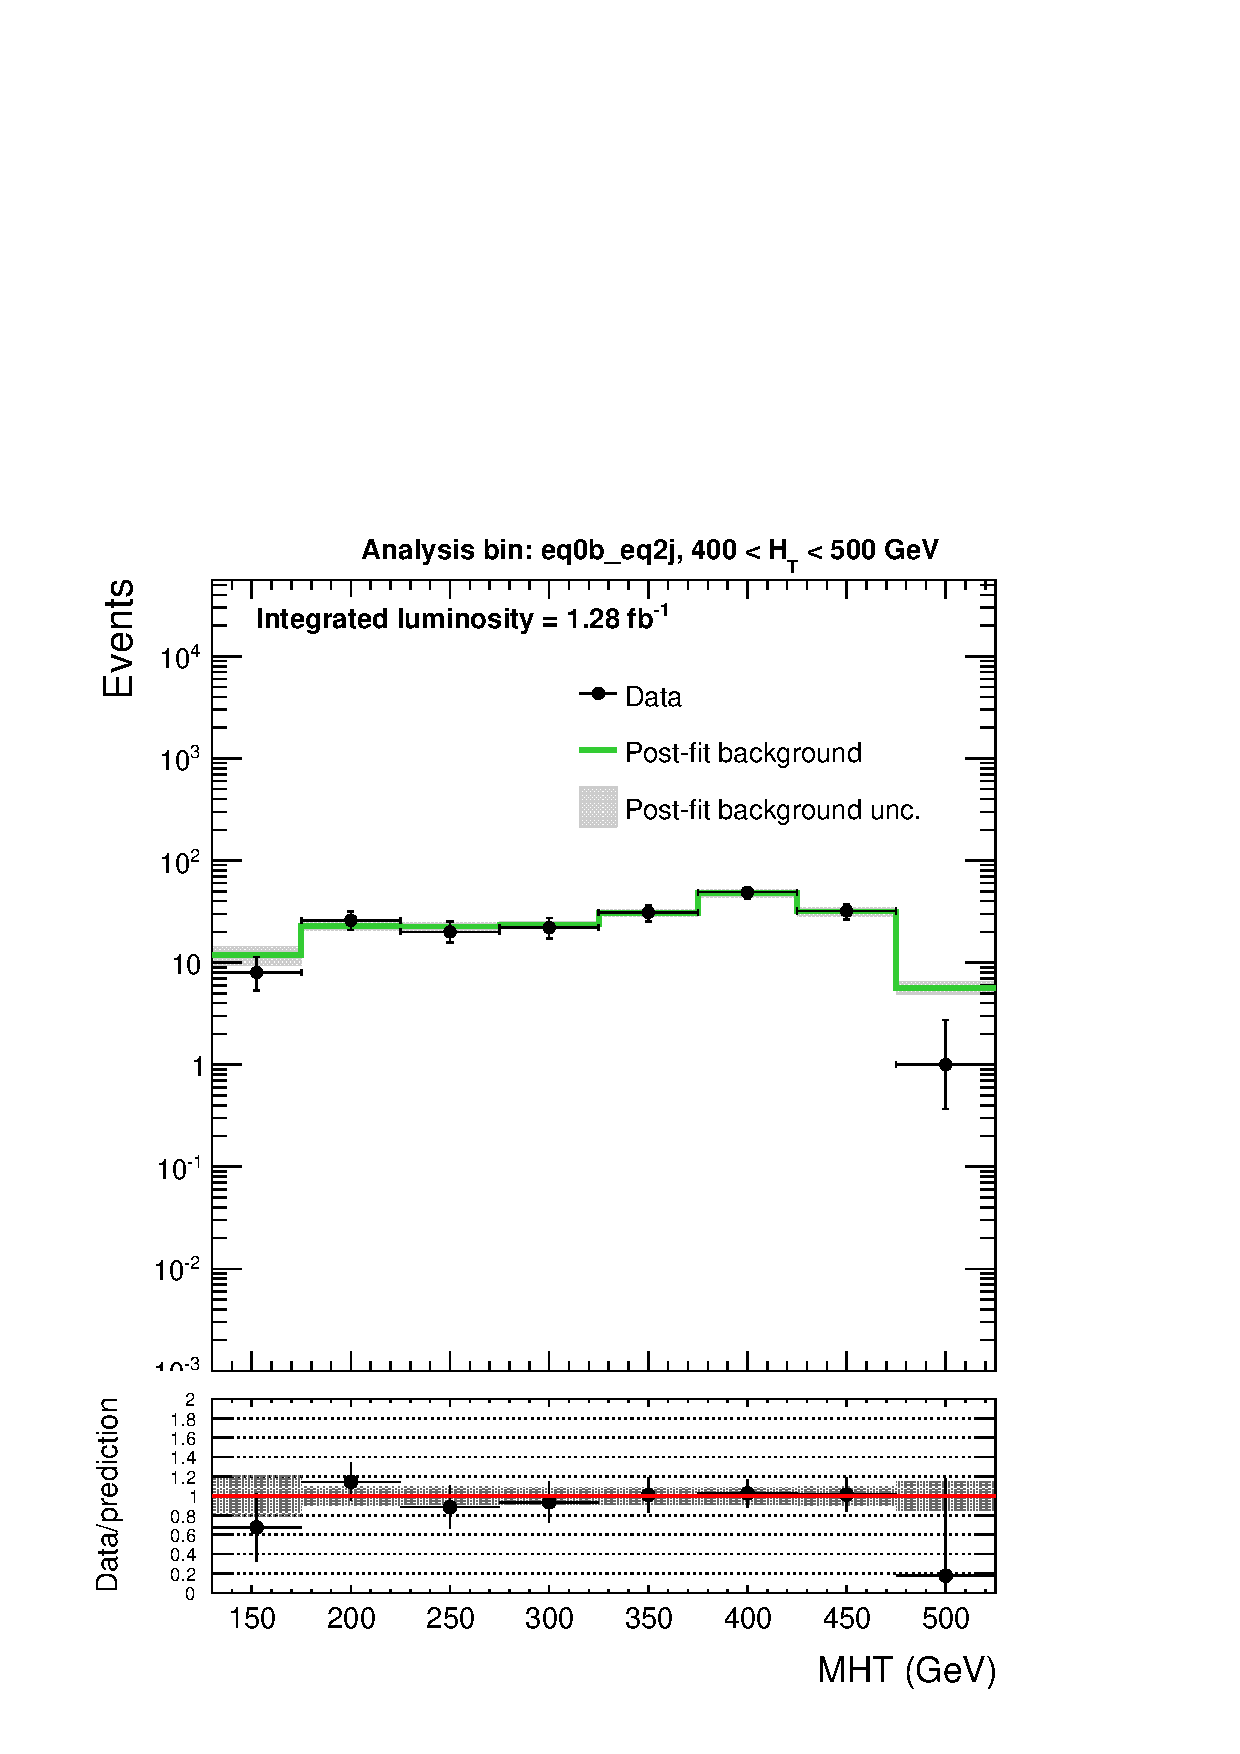
\includegraphics[width=0.25\textwidth]{figures/postFitResults/postFitShape_eq0b_eq2j_400_500.pdf} }\hspace{1cm}
    \subfigure[$\nj^{\mathrm{sym}}=2$, $\nb=0$, $500 < \scalht < 600 \; \mathrm{GeV}$]{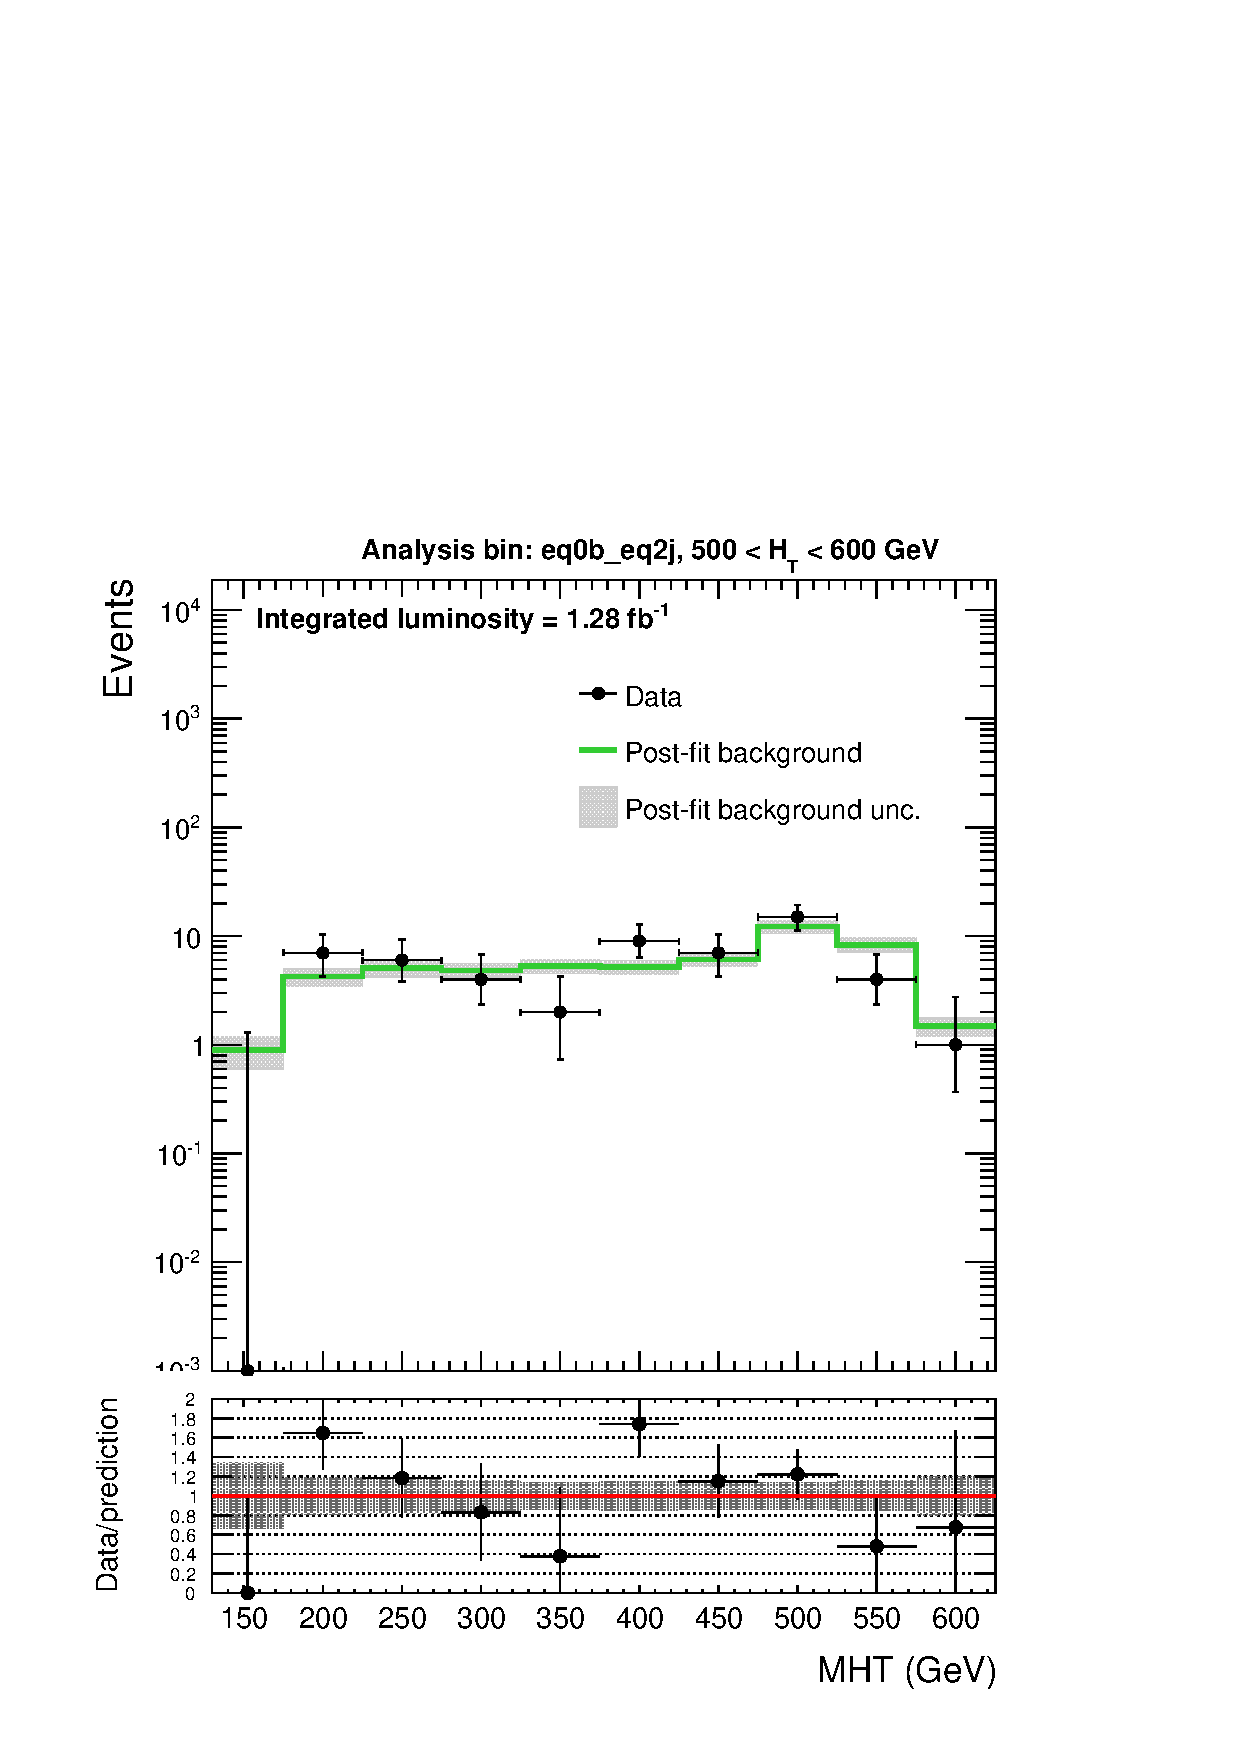
\includegraphics[width=0.25\textwidth]{figures/postFitResults/postFitShape_eq0b_eq2j_500_600.pdf} }\\
    \subfigure[$\nj^{\mathrm{sym}}=2$, $\nb=0$, $600 < \scalht < 800 \; \mathrm{GeV}$]{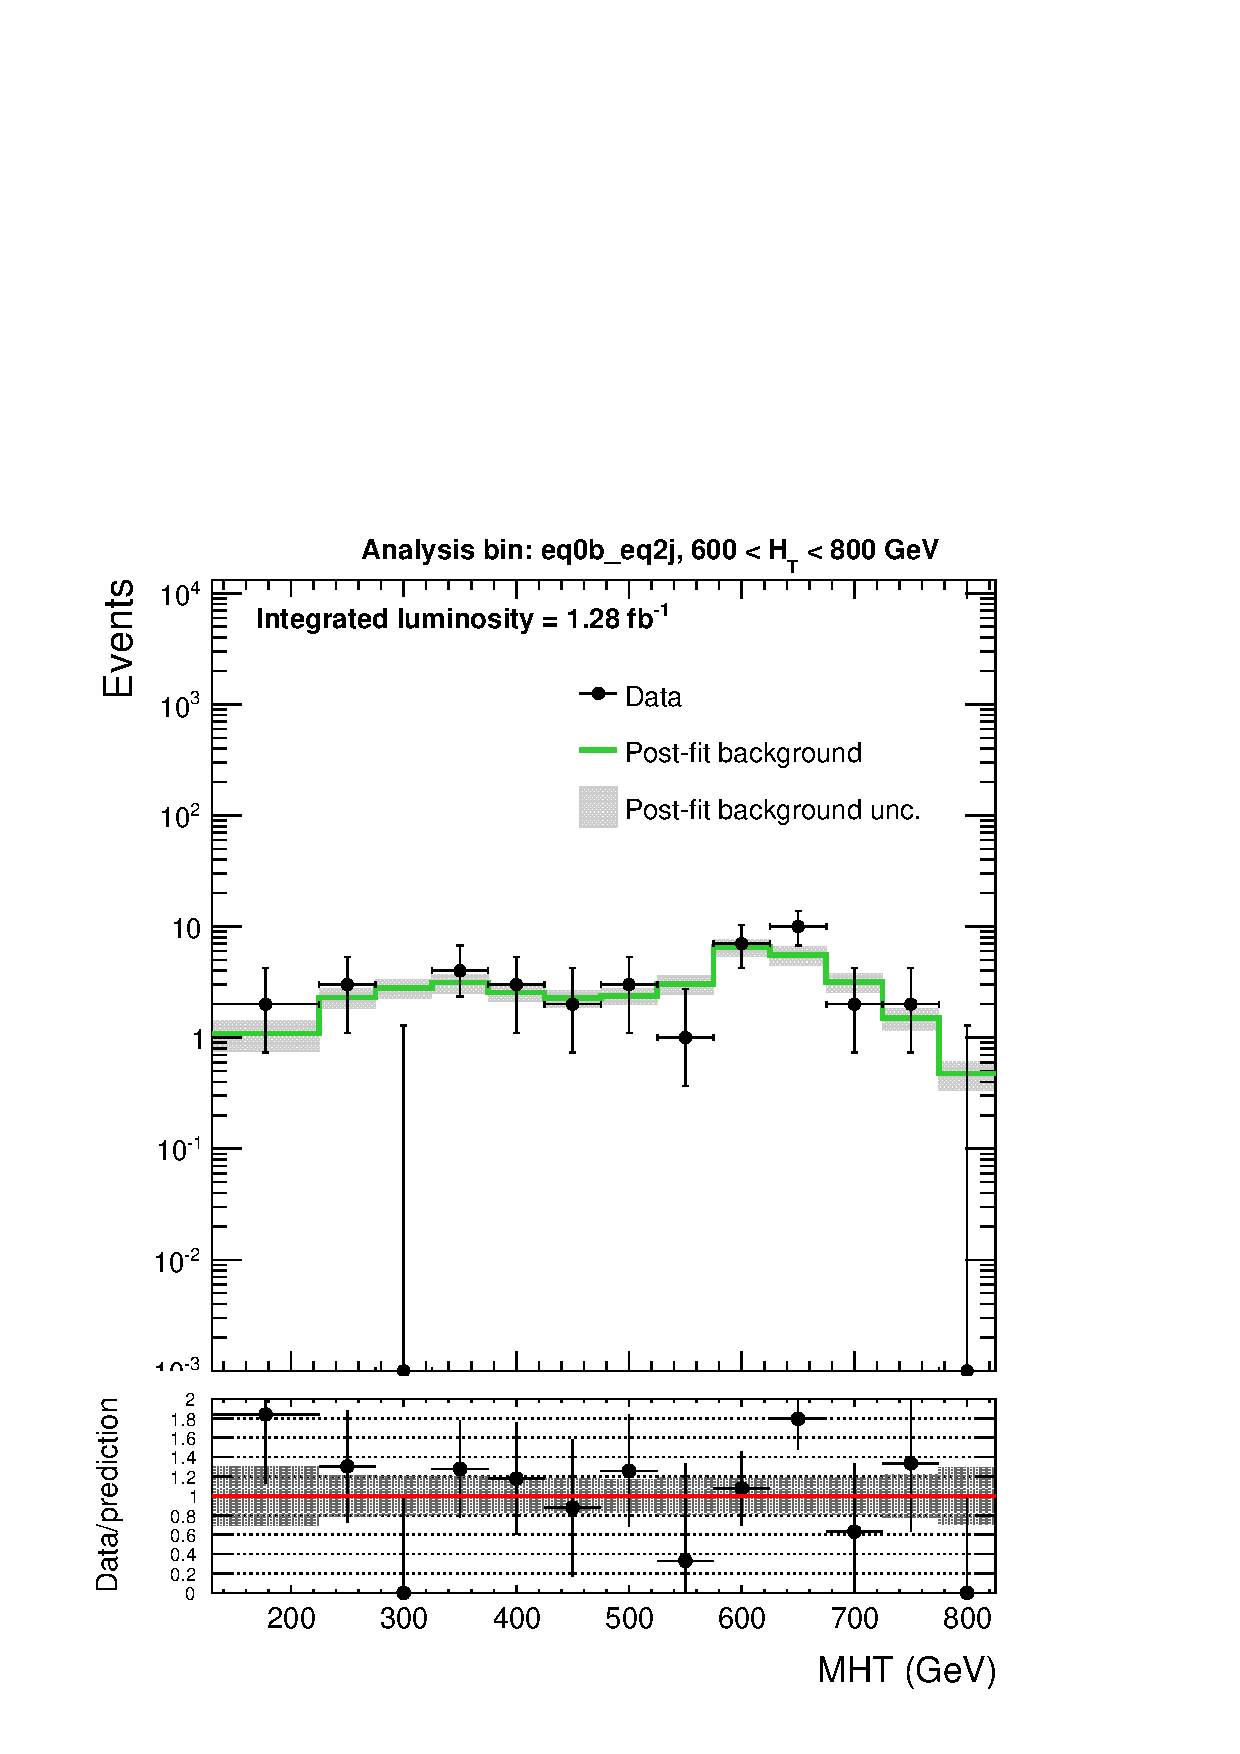
\includegraphics[width=0.25\textwidth]{figures/postFitResults/postFitShape_eq0b_eq2j_600_800.pdf} }\hspace{1cm}
    \subfigure[$\nj^{\mathrm{sym}}=2$, $\nb=0$, $\scalht > 800 \; \mathrm{GeV}$]{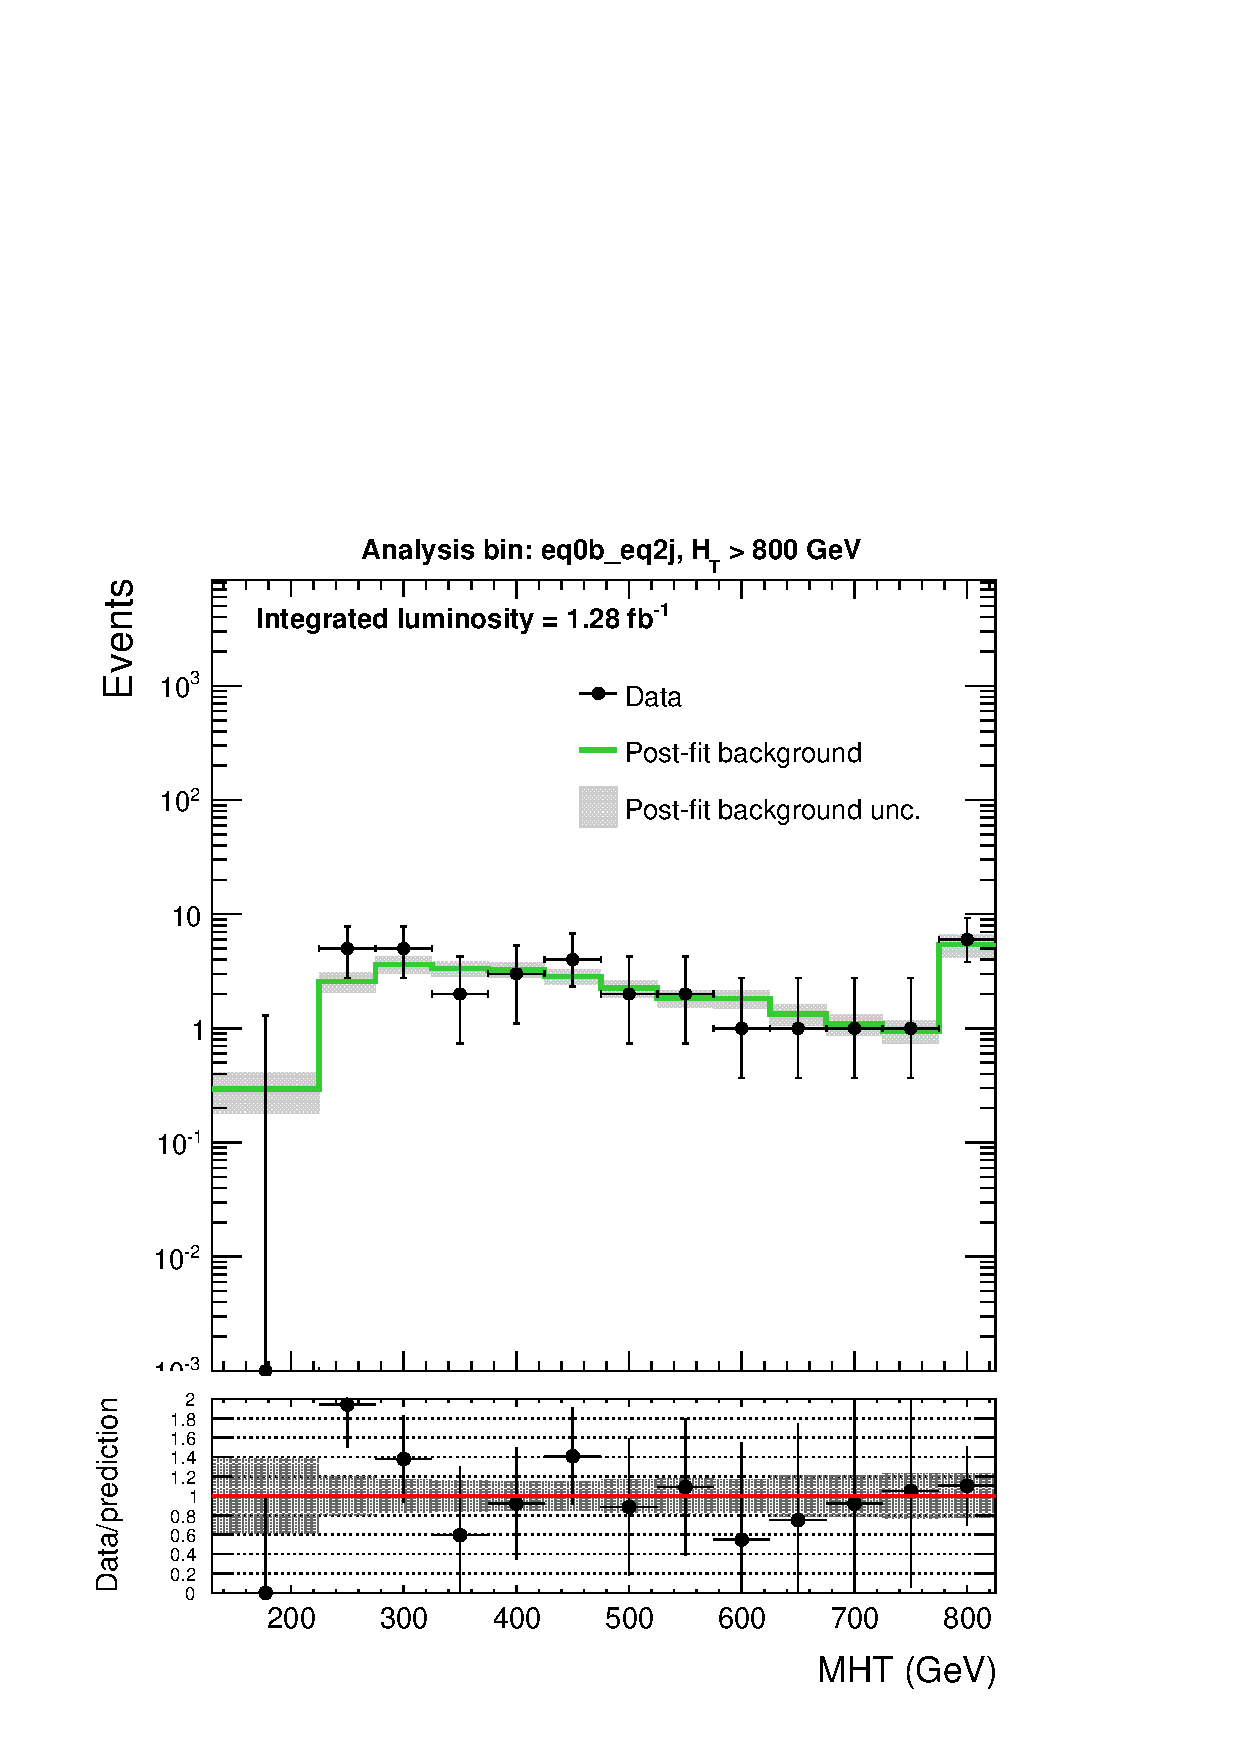
\includegraphics[width=0.25\textwidth]{figures/postFitResults/postFitShape_eq0b_eq2j_800_Inf.pdf} }\hspace{1cm}
  \end{center}
\end{figure}



\newpage
\begin{figure}[h!]
\caption{Post-fit \MHT templates for the bin $\nj^{\mathrm{asym}}=3$, $\nb=0$ \label{fig:postFitShapes_eq0b_eq3a}}.
\begin{center}

    \subfigure[$\nj^{\mathrm{asym}}=3$, $\nb=0$, $200 < \scalht < 250 \; \mathrm{GeV}$]{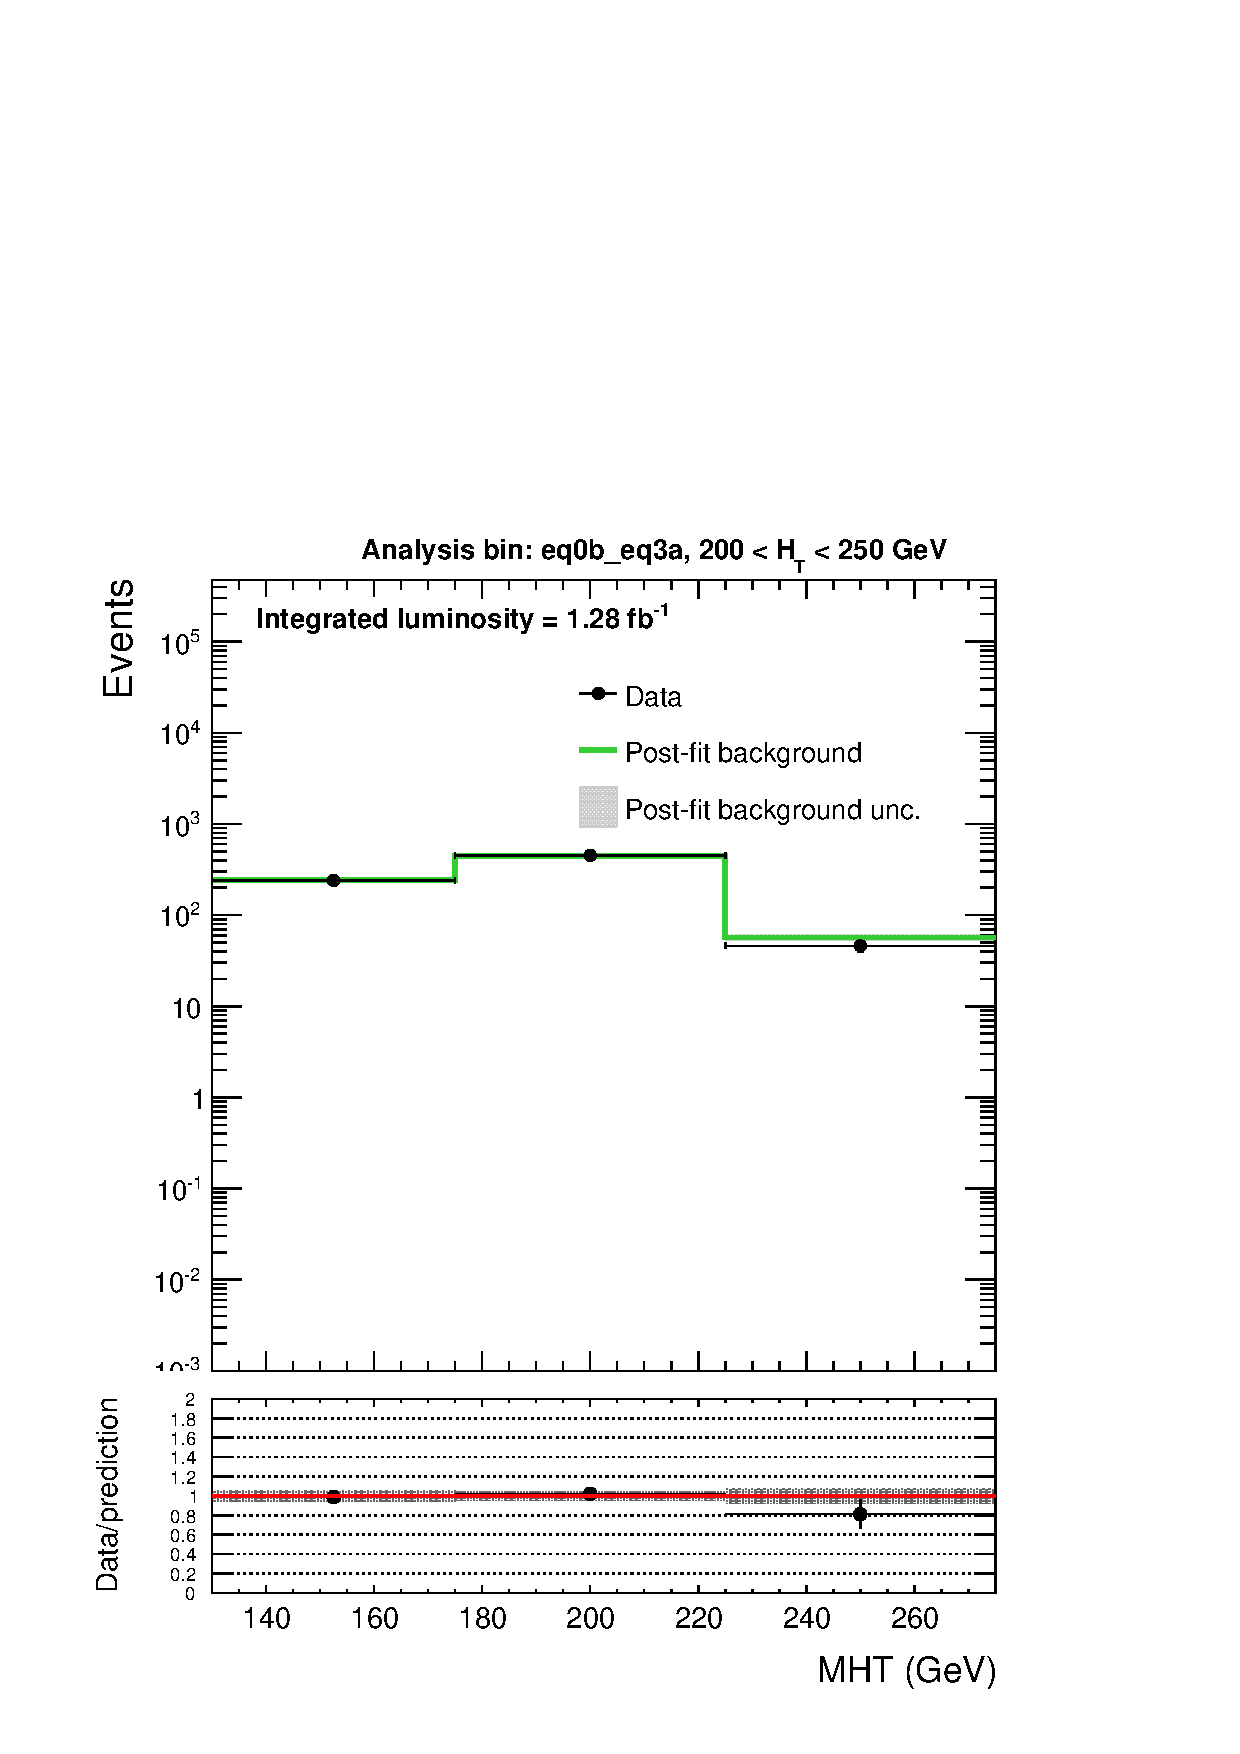
\includegraphics[width=0.25\textwidth]{figures/postFitResults/postFitShape_eq0b_eq3a_200_250.pdf} }\hspace{1cm}
    \subfigure[$\nj^{\mathrm{asym}}=3$, $\nb=0$, $250 < \scalht < 300 \; \mathrm{GeV}$]{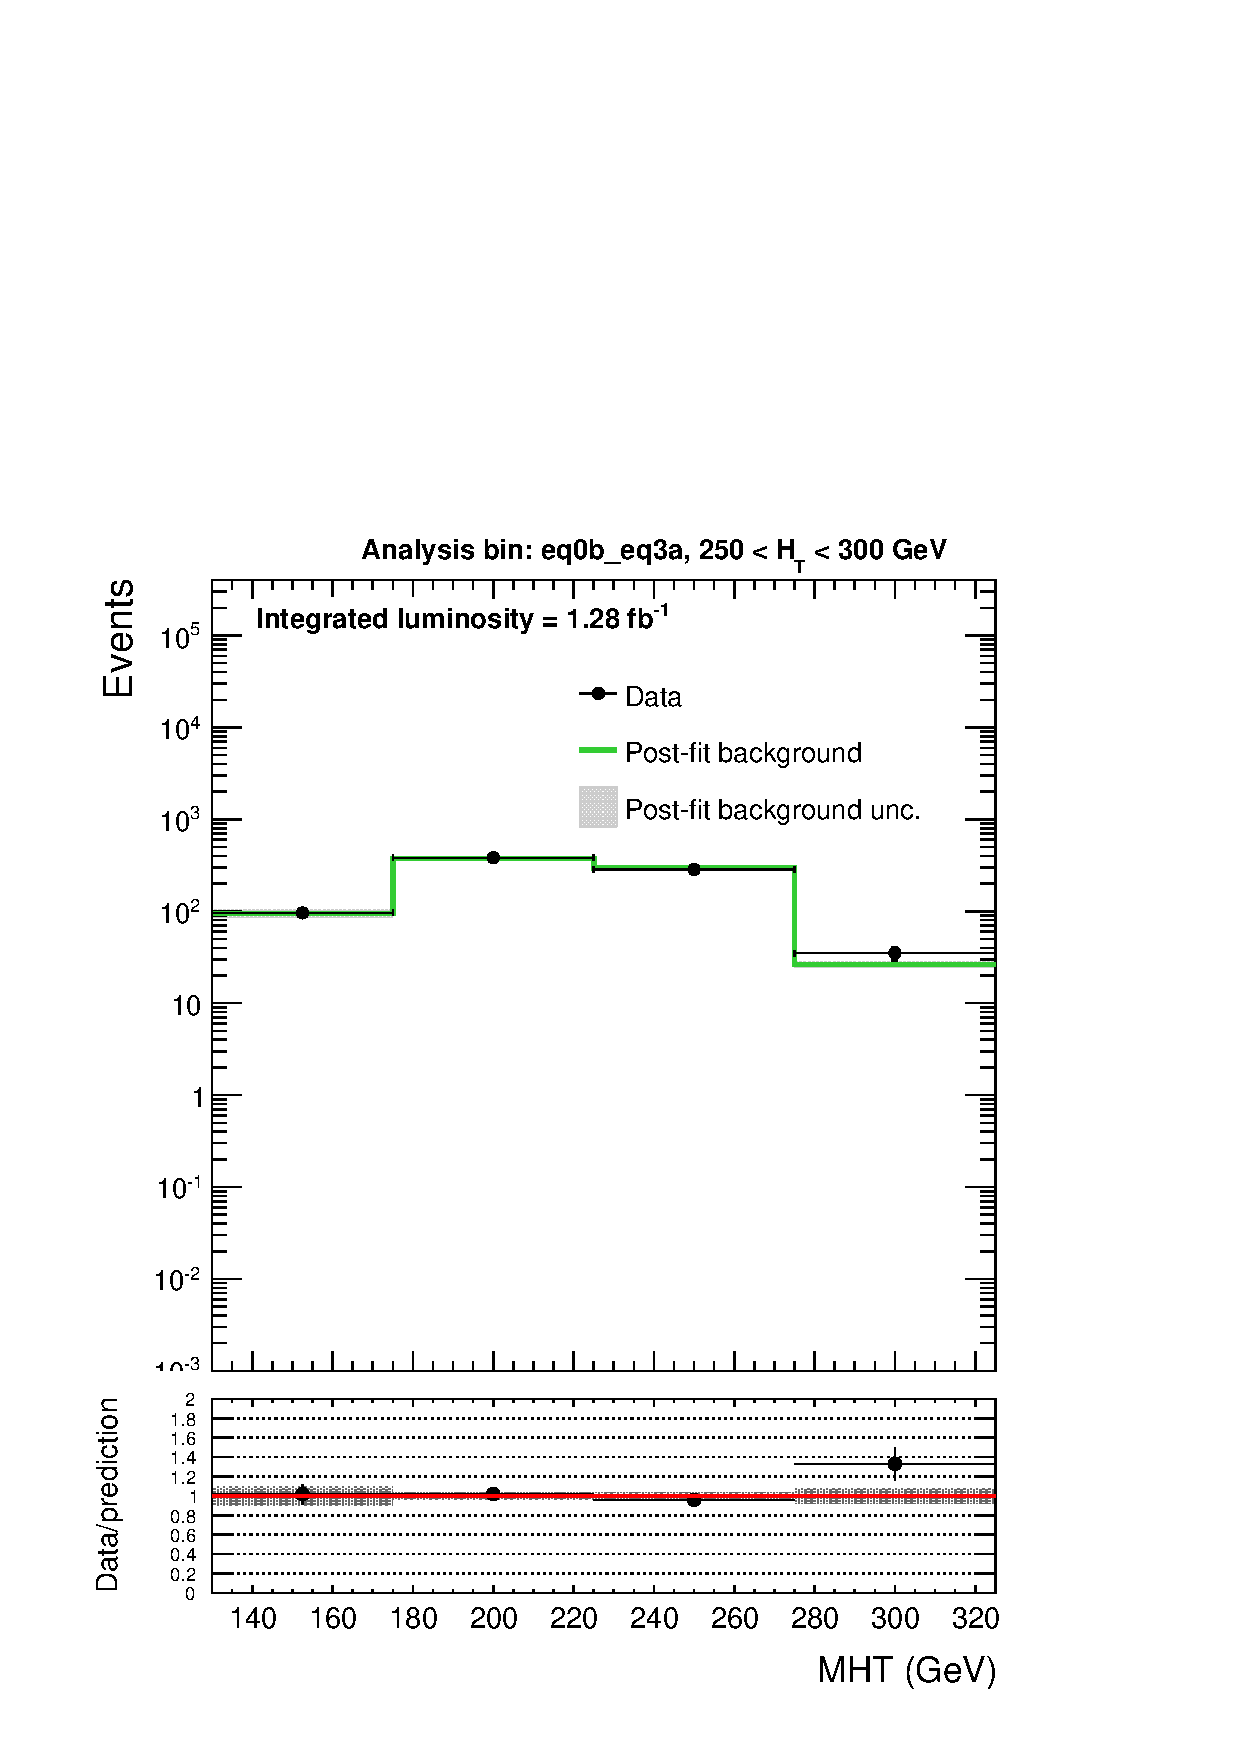
\includegraphics[width=0.25\textwidth]{figures/postFitResults/postFitShape_eq0b_eq3a_250_300.pdf} }\hspace{1cm}
    \subfigure[$\nj^{\mathrm{asym}}=3$, $\nb=0$, $300 < \scalht < 350 \; \mathrm{GeV}$]{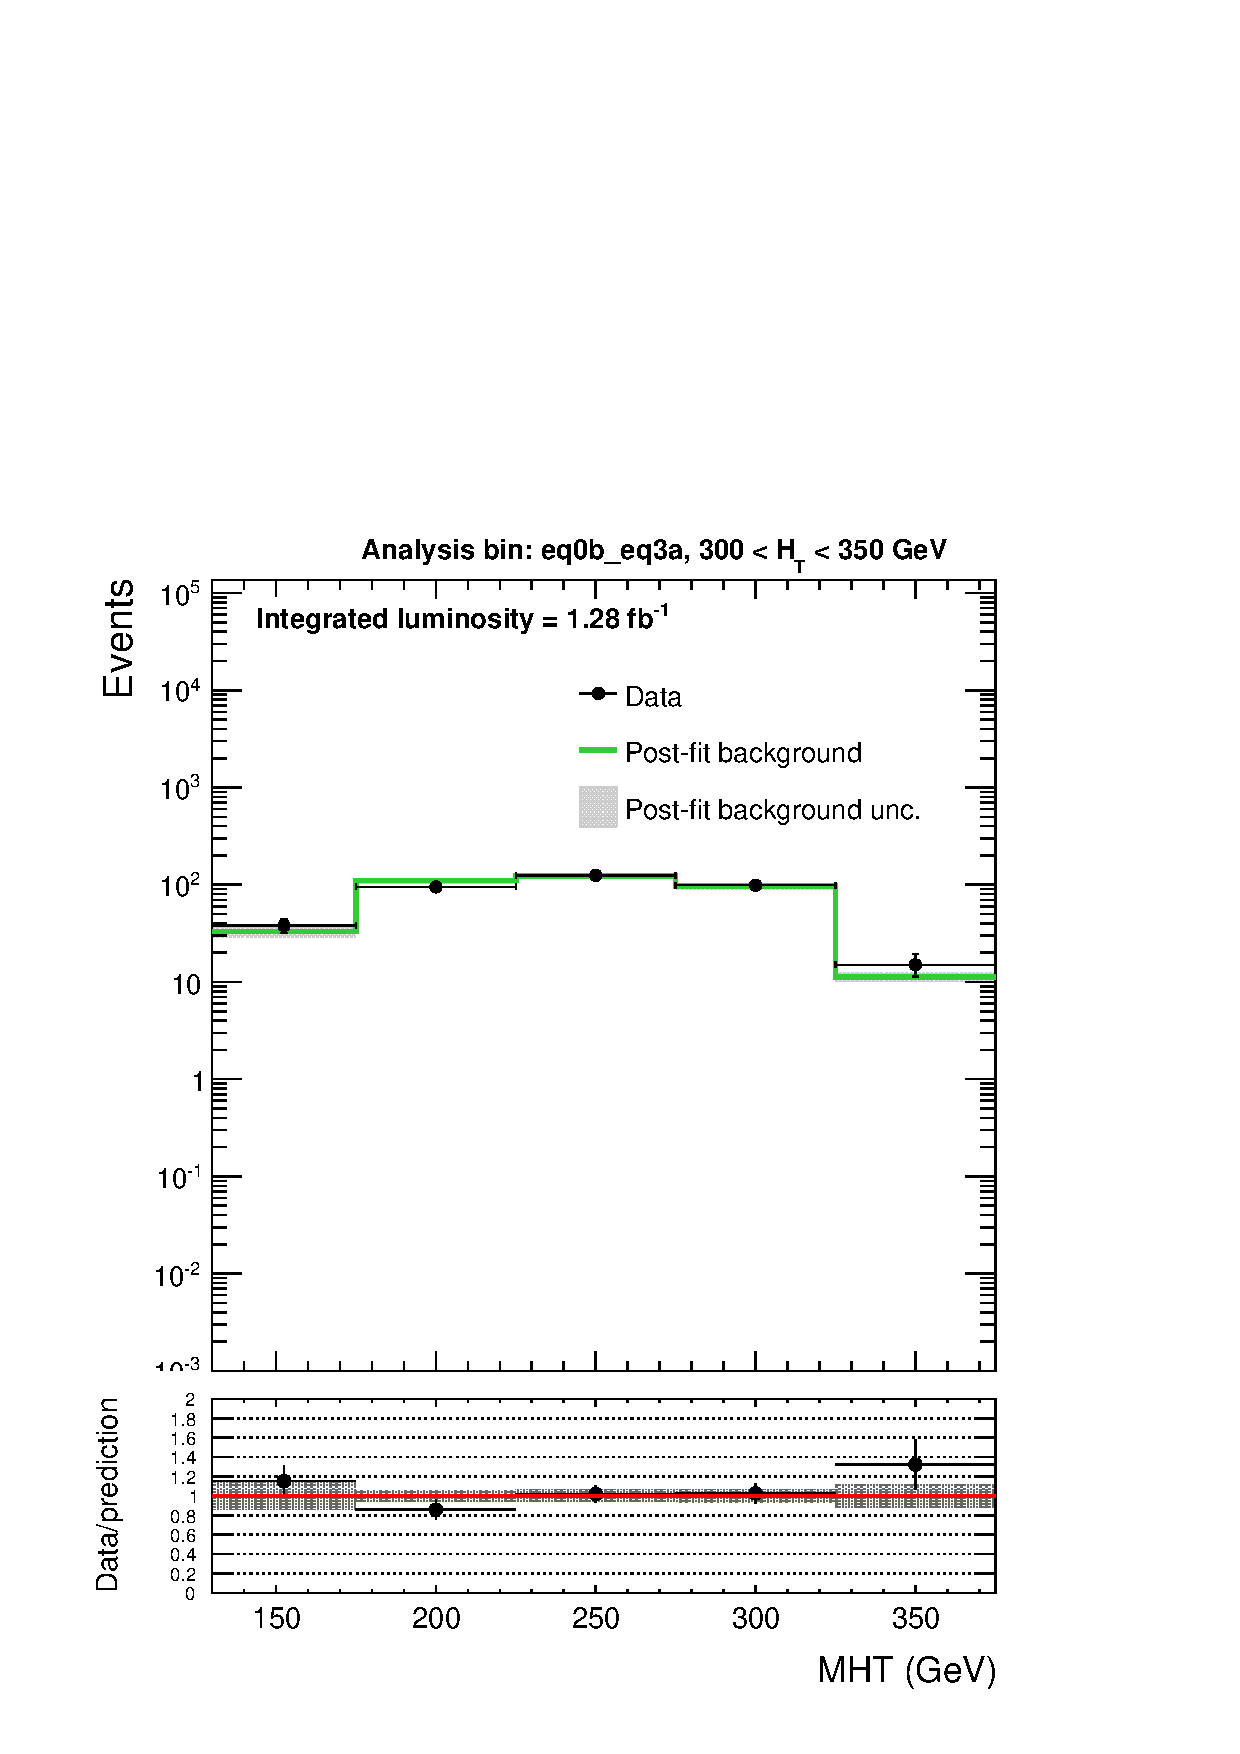
\includegraphics[width=0.25\textwidth]{figures/postFitResults/postFitShape_eq0b_eq3a_300_350.pdf} }\\
    \subfigure[$\nj^{\mathrm{asym}}=3$, $\nb=0$, $350 < \scalht < 400 \; \mathrm{GeV}$]{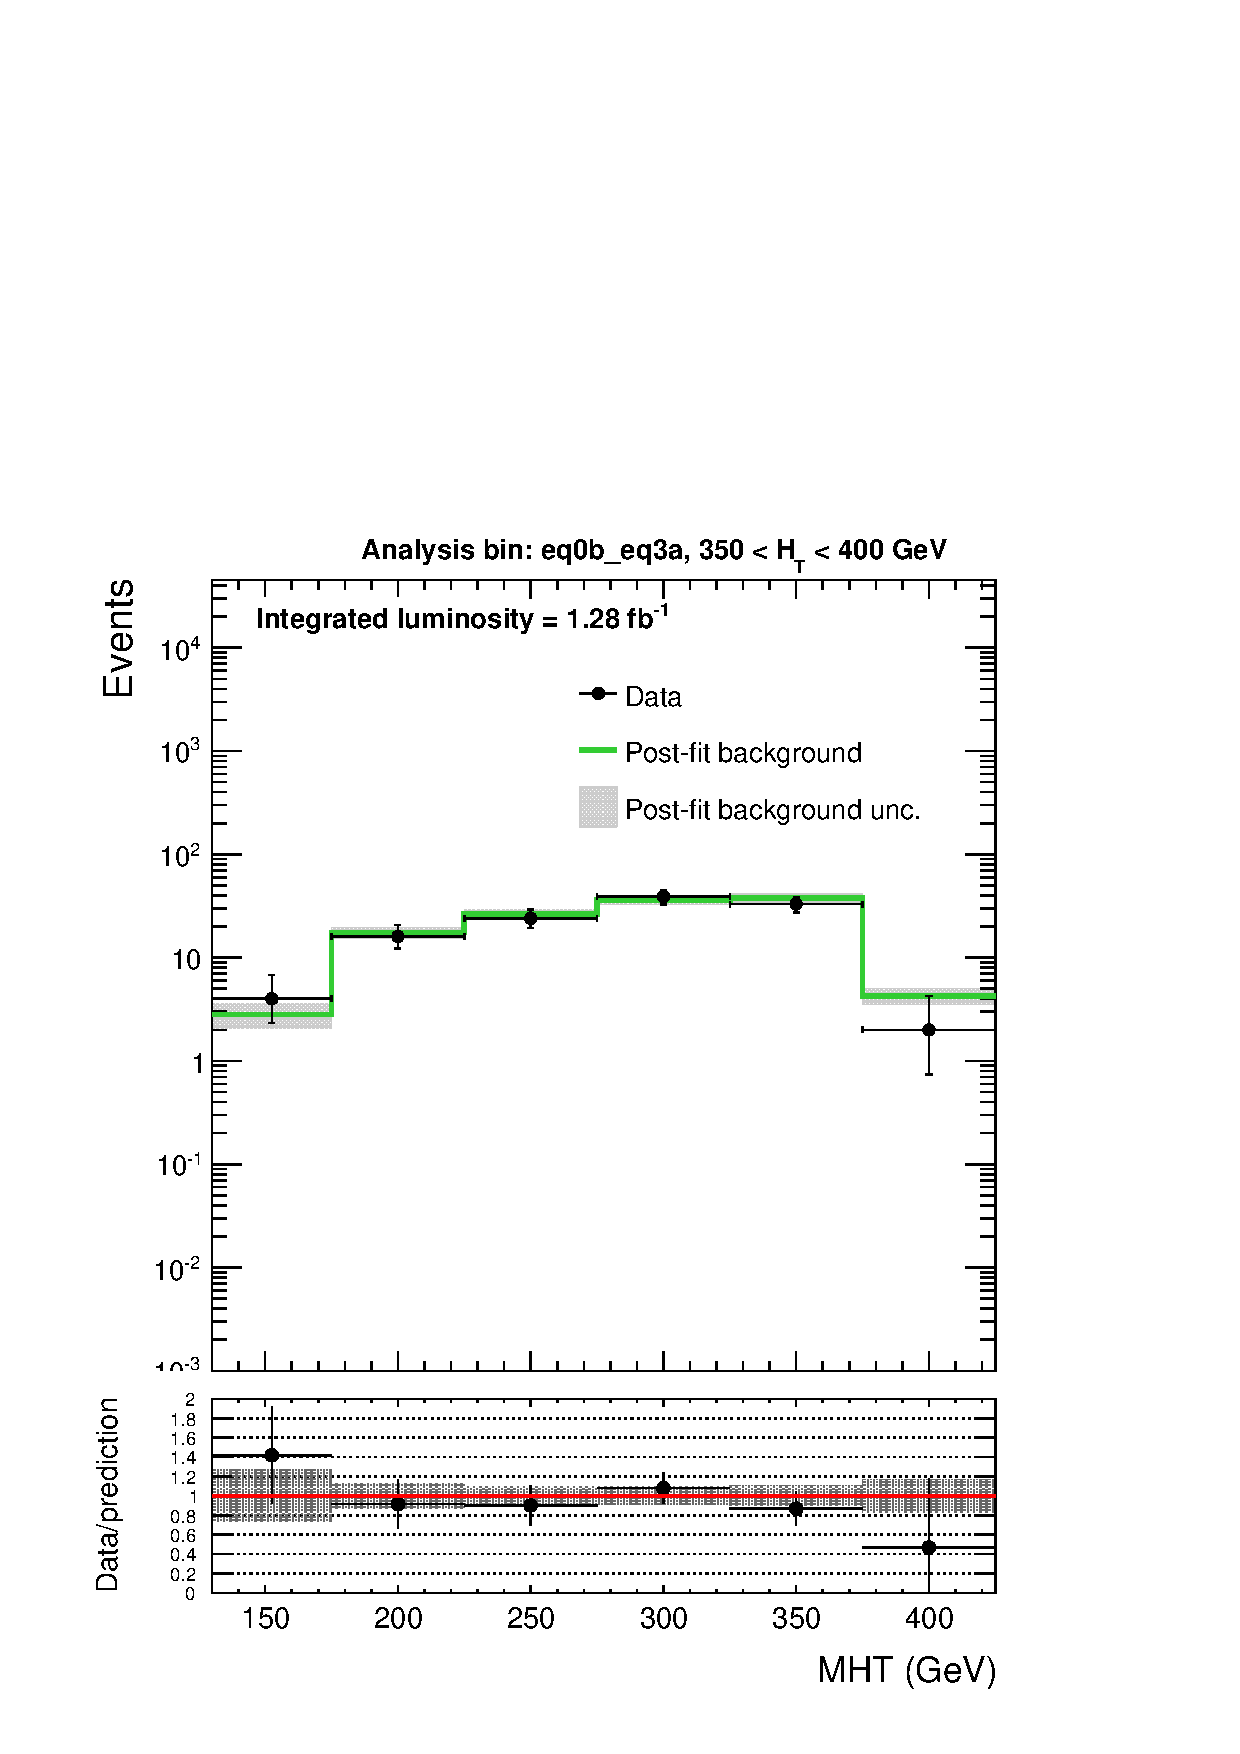
\includegraphics[width=0.25\textwidth]{figures/postFitResults/postFitShape_eq0b_eq3a_350_400.pdf} }\hspace{1cm}
    \subfigure[$\nj^{\mathrm{asym}}=3$, $\nb=0$, $400 < \scalht < 500 \; \mathrm{GeV}$]{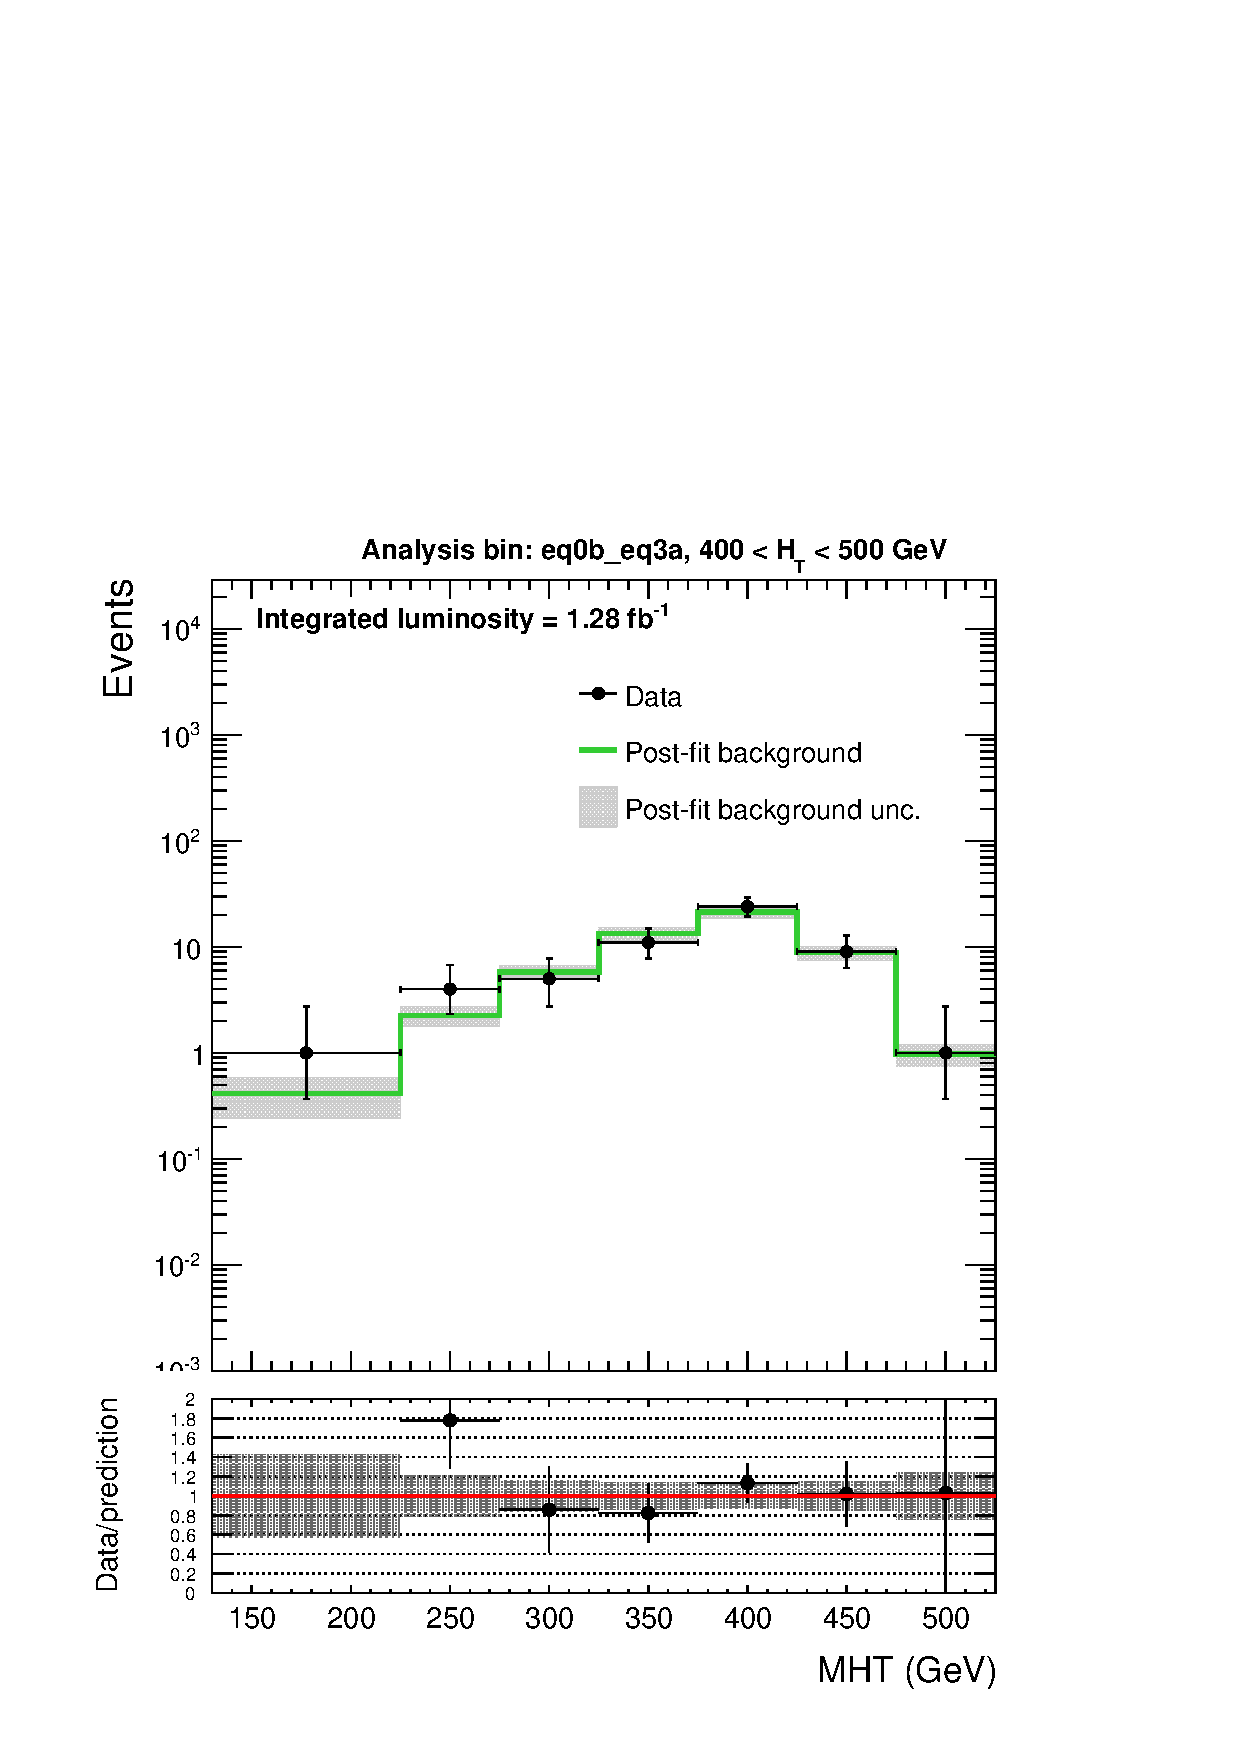
\includegraphics[width=0.25\textwidth]{figures/postFitResults/postFitShape_eq0b_eq3a_400_500.pdf} }\hspace{1cm}
    \subfigure[$\nj^{\mathrm{asym}}=3$, $\nb=0$, $500 < \scalht < 600 \; \mathrm{GeV}$]{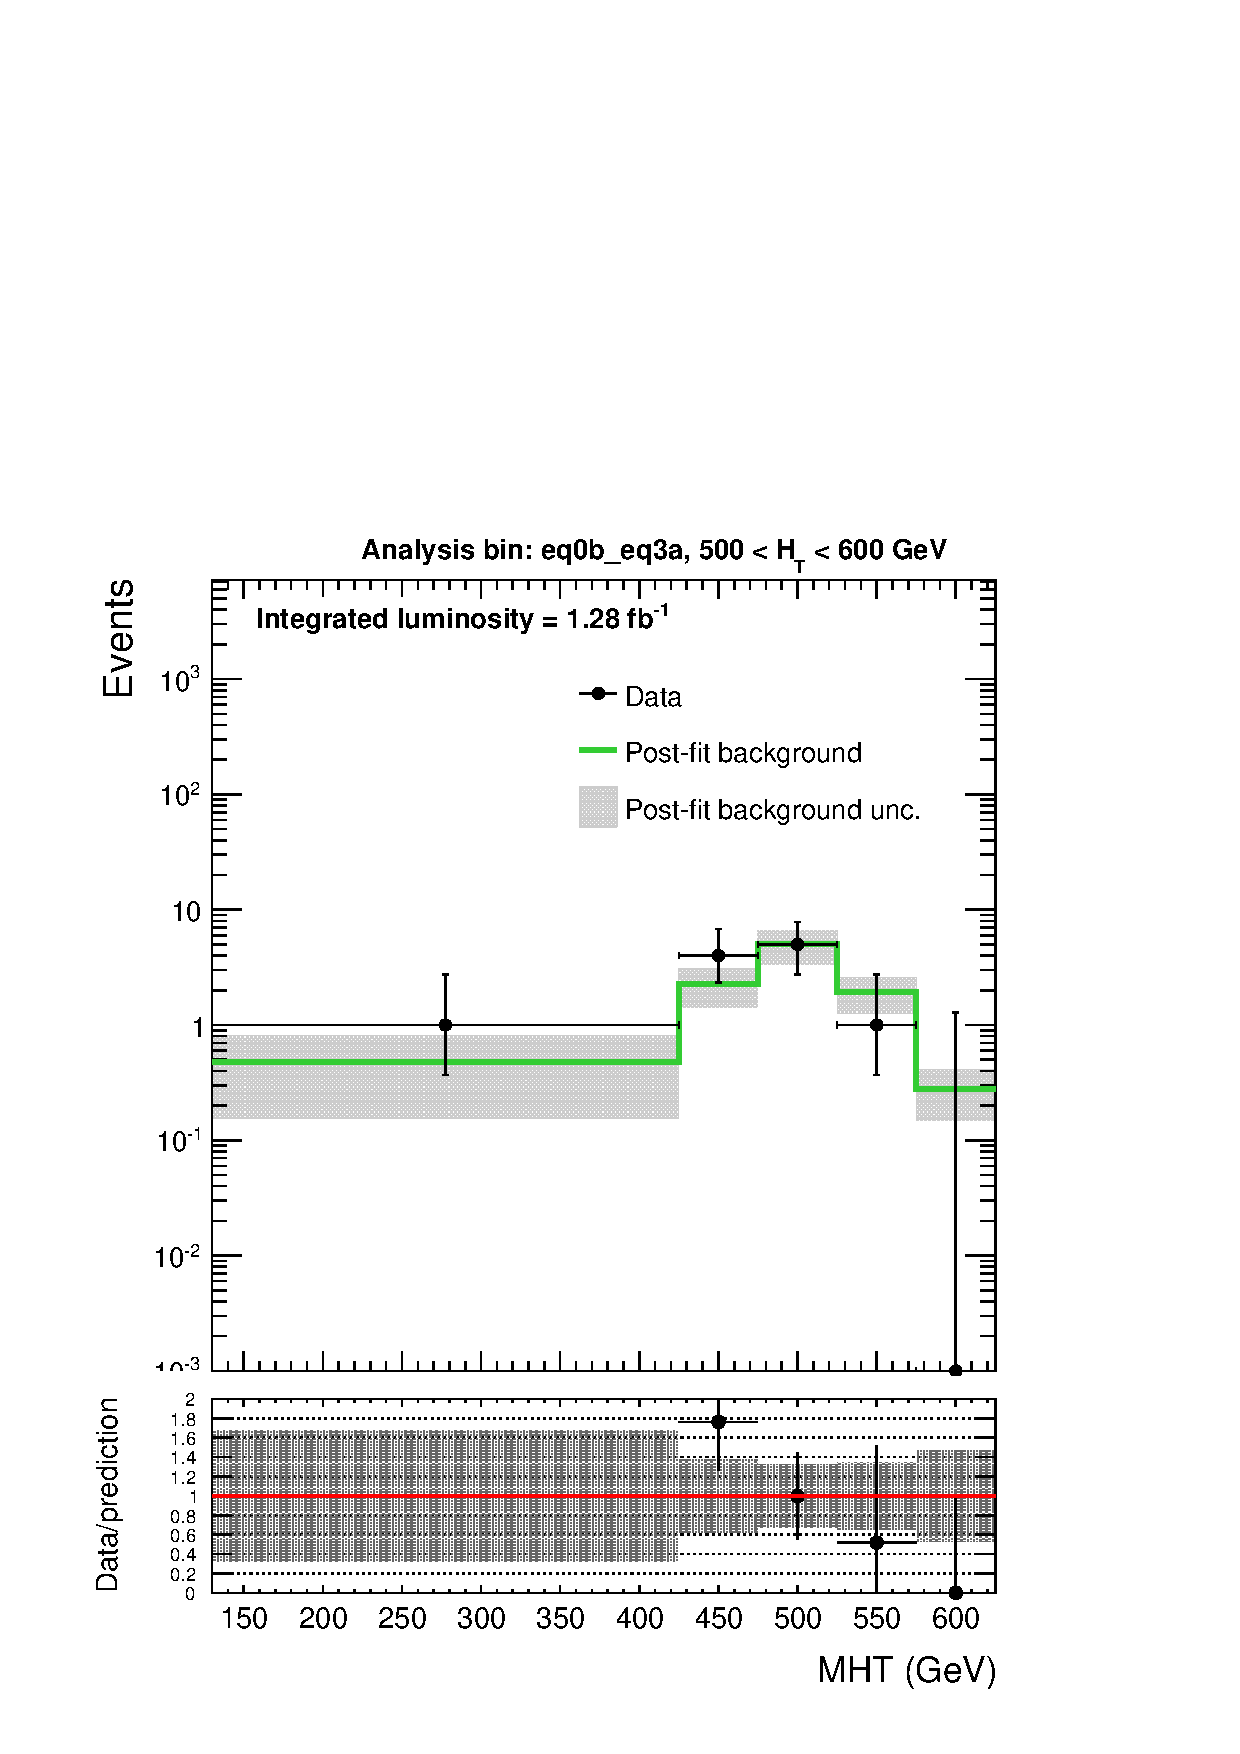
\includegraphics[width=0.25\textwidth]{figures/postFitResults/postFitShape_eq0b_eq3a_500_600.pdf} }\\
    \subfigure[$\nj^{\mathrm{asym}}=3$, $\nb=0$, $\scalht > 600 \; \mathrm{GeV}$]{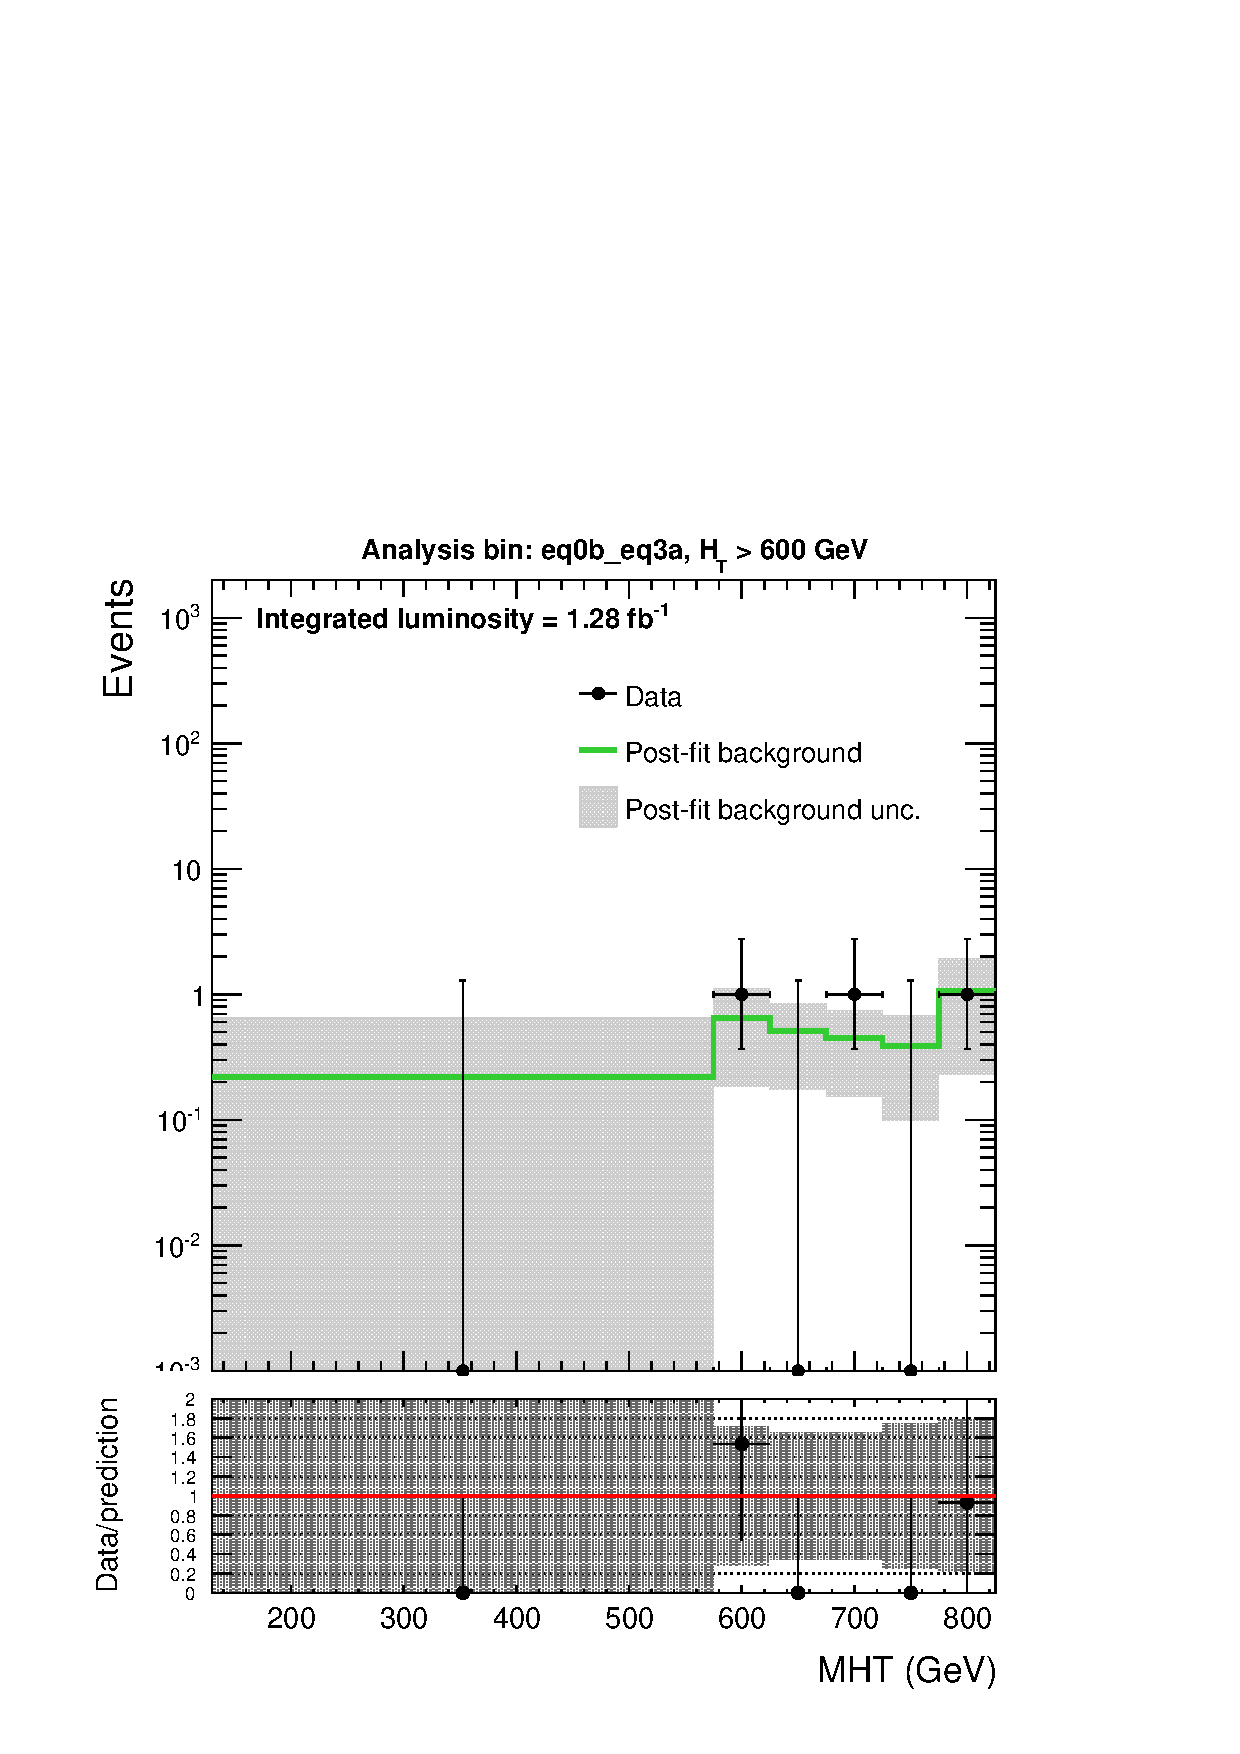
\includegraphics[width=0.25\textwidth]{figures/postFitResults/postFitShape_eq0b_eq3a_600_Inf.pdf} }\hspace{1cm}
  \end{center}
\end{figure}



\newpage
\begin{figure}[h!]
\caption{Post-fit \MHT templates for the bin $\nj^{\mathrm{sym}}=3$, $\nb=0$ \label{fig:postFitShapes_eq0b_eq3j}}.
\begin{center}

    \subfigure[$\nj^{\mathrm{sym}}=3$, $\nb=0$, $250 < \scalht < 300 \; \mathrm{GeV}$]{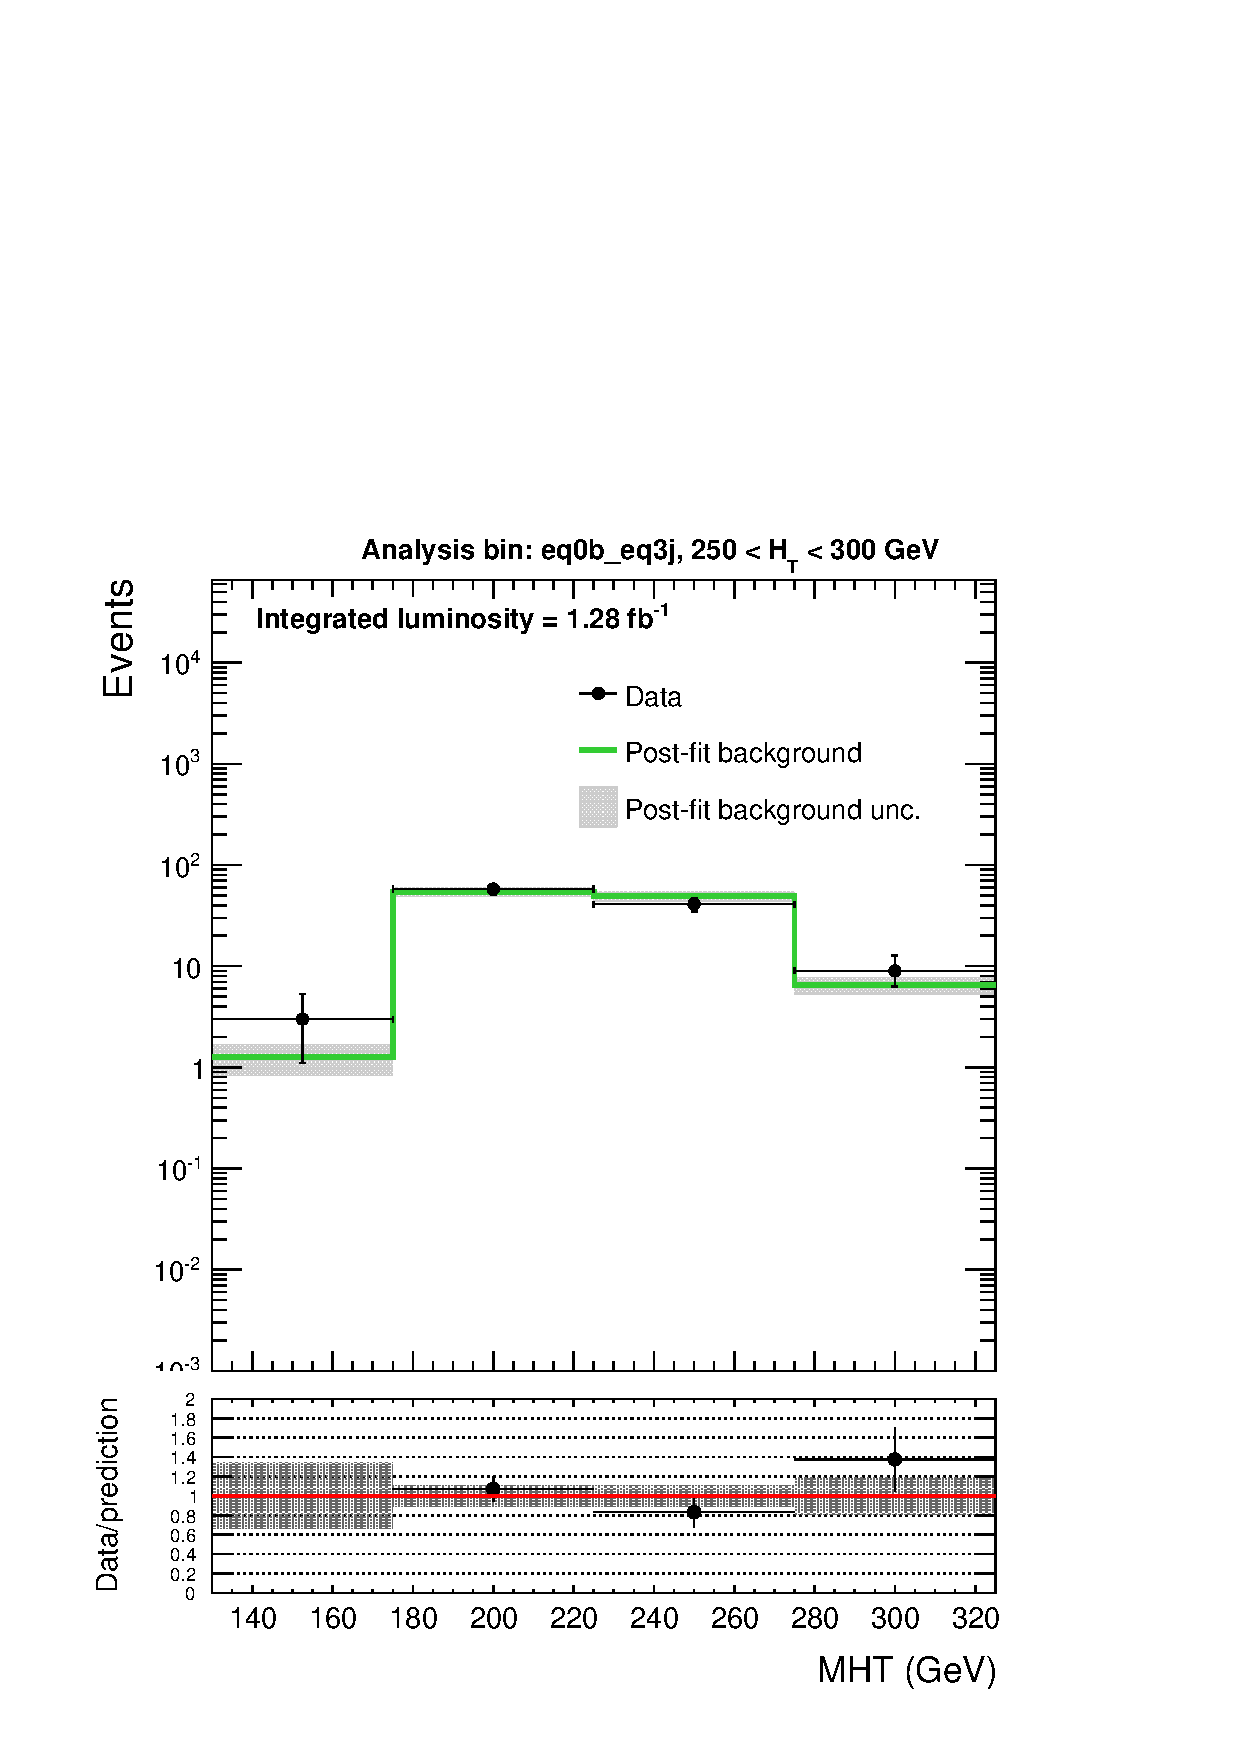
\includegraphics[width=0.25\textwidth]{figures/postFitResults/postFitShape_eq0b_eq3j_250_300.pdf} }\hspace{1cm}
    \subfigure[$\nj^{\mathrm{sym}}=3$, $\nb=0$, $300 < \scalht < 350 \; \mathrm{GeV}$]{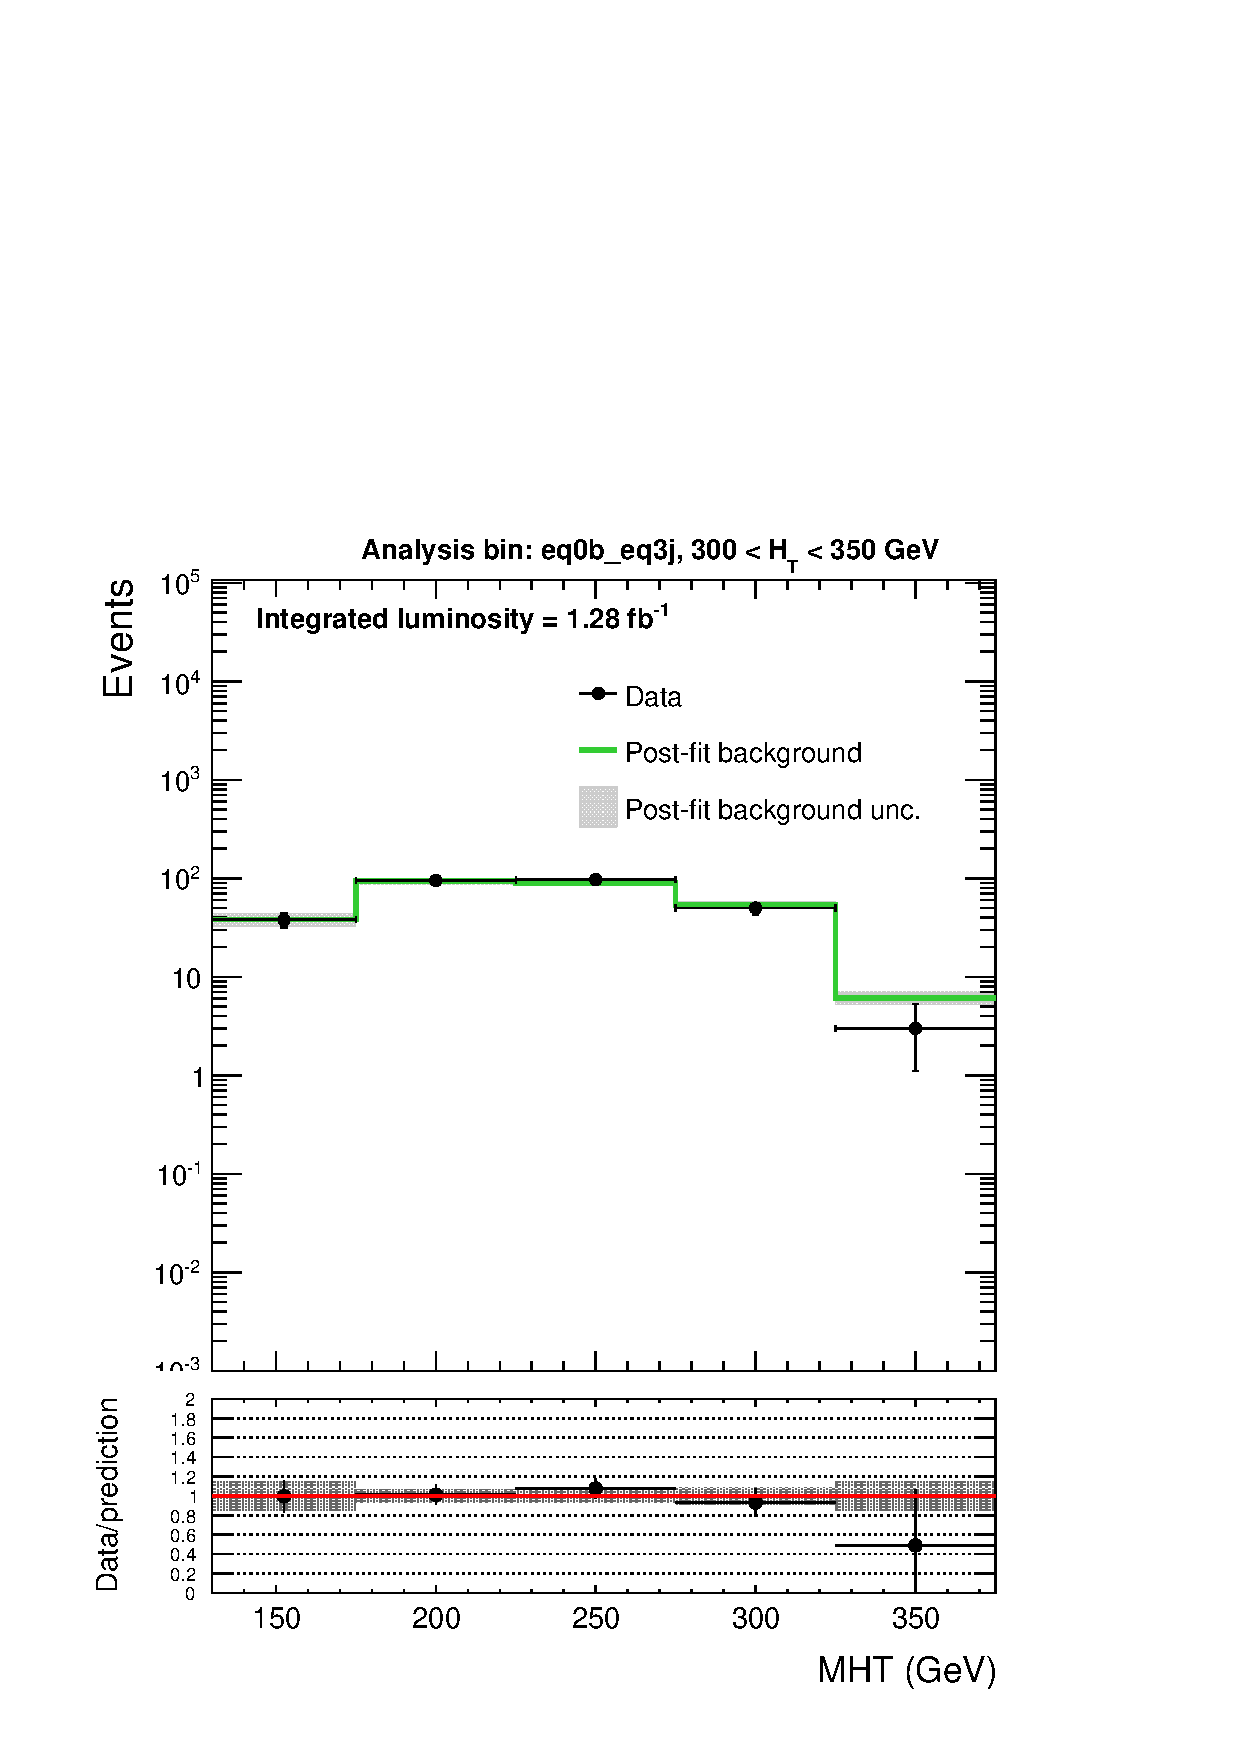
\includegraphics[width=0.25\textwidth]{figures/postFitResults/postFitShape_eq0b_eq3j_300_350.pdf} }\hspace{1cm}
    \subfigure[$\nj^{\mathrm{sym}}=3$, $\nb=0$, $350 < \scalht < 400 \; \mathrm{GeV}$]{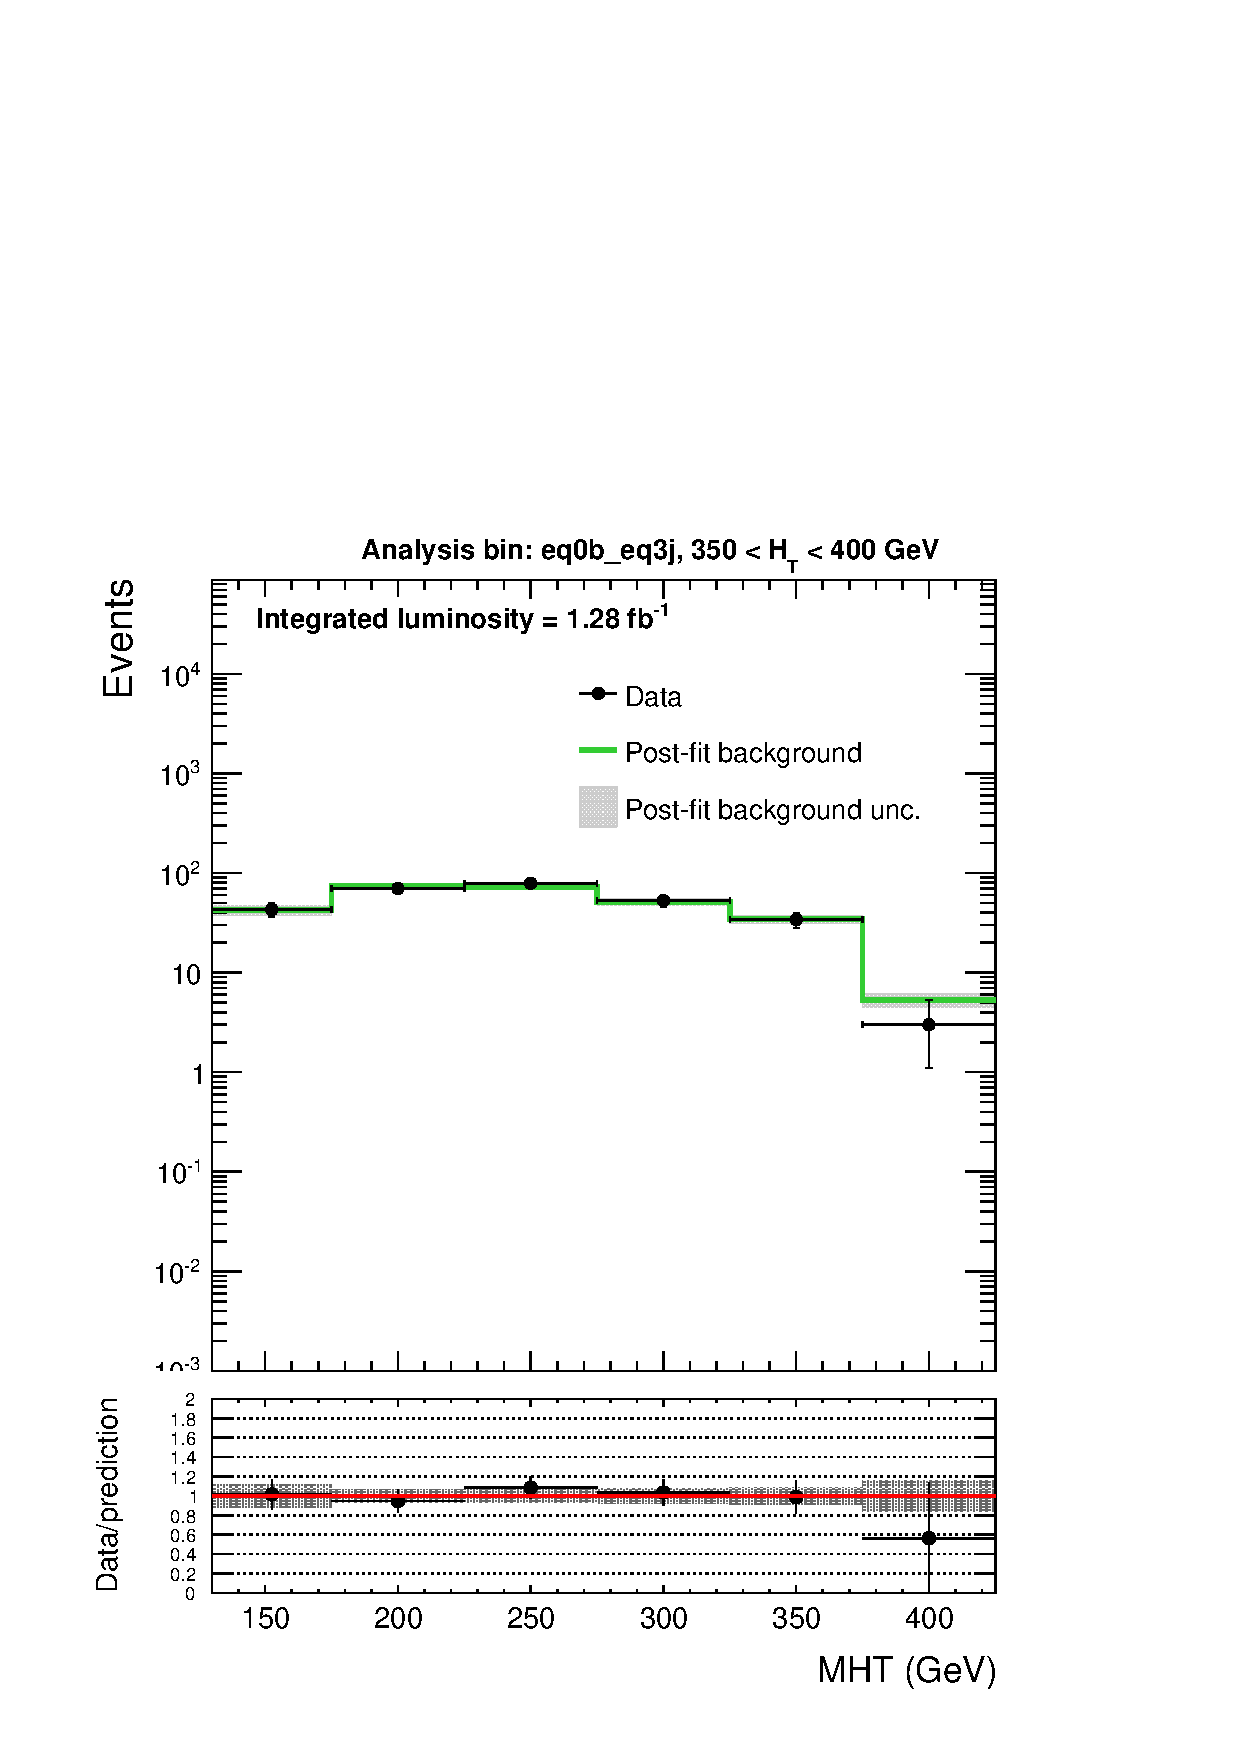
\includegraphics[width=0.25\textwidth]{figures/postFitResults/postFitShape_eq0b_eq3j_350_400.pdf} }\\
    \subfigure[$\nj^{\mathrm{sym}}=3$, $\nb=0$, $400 < \scalht < 500 \; \mathrm{GeV}$]{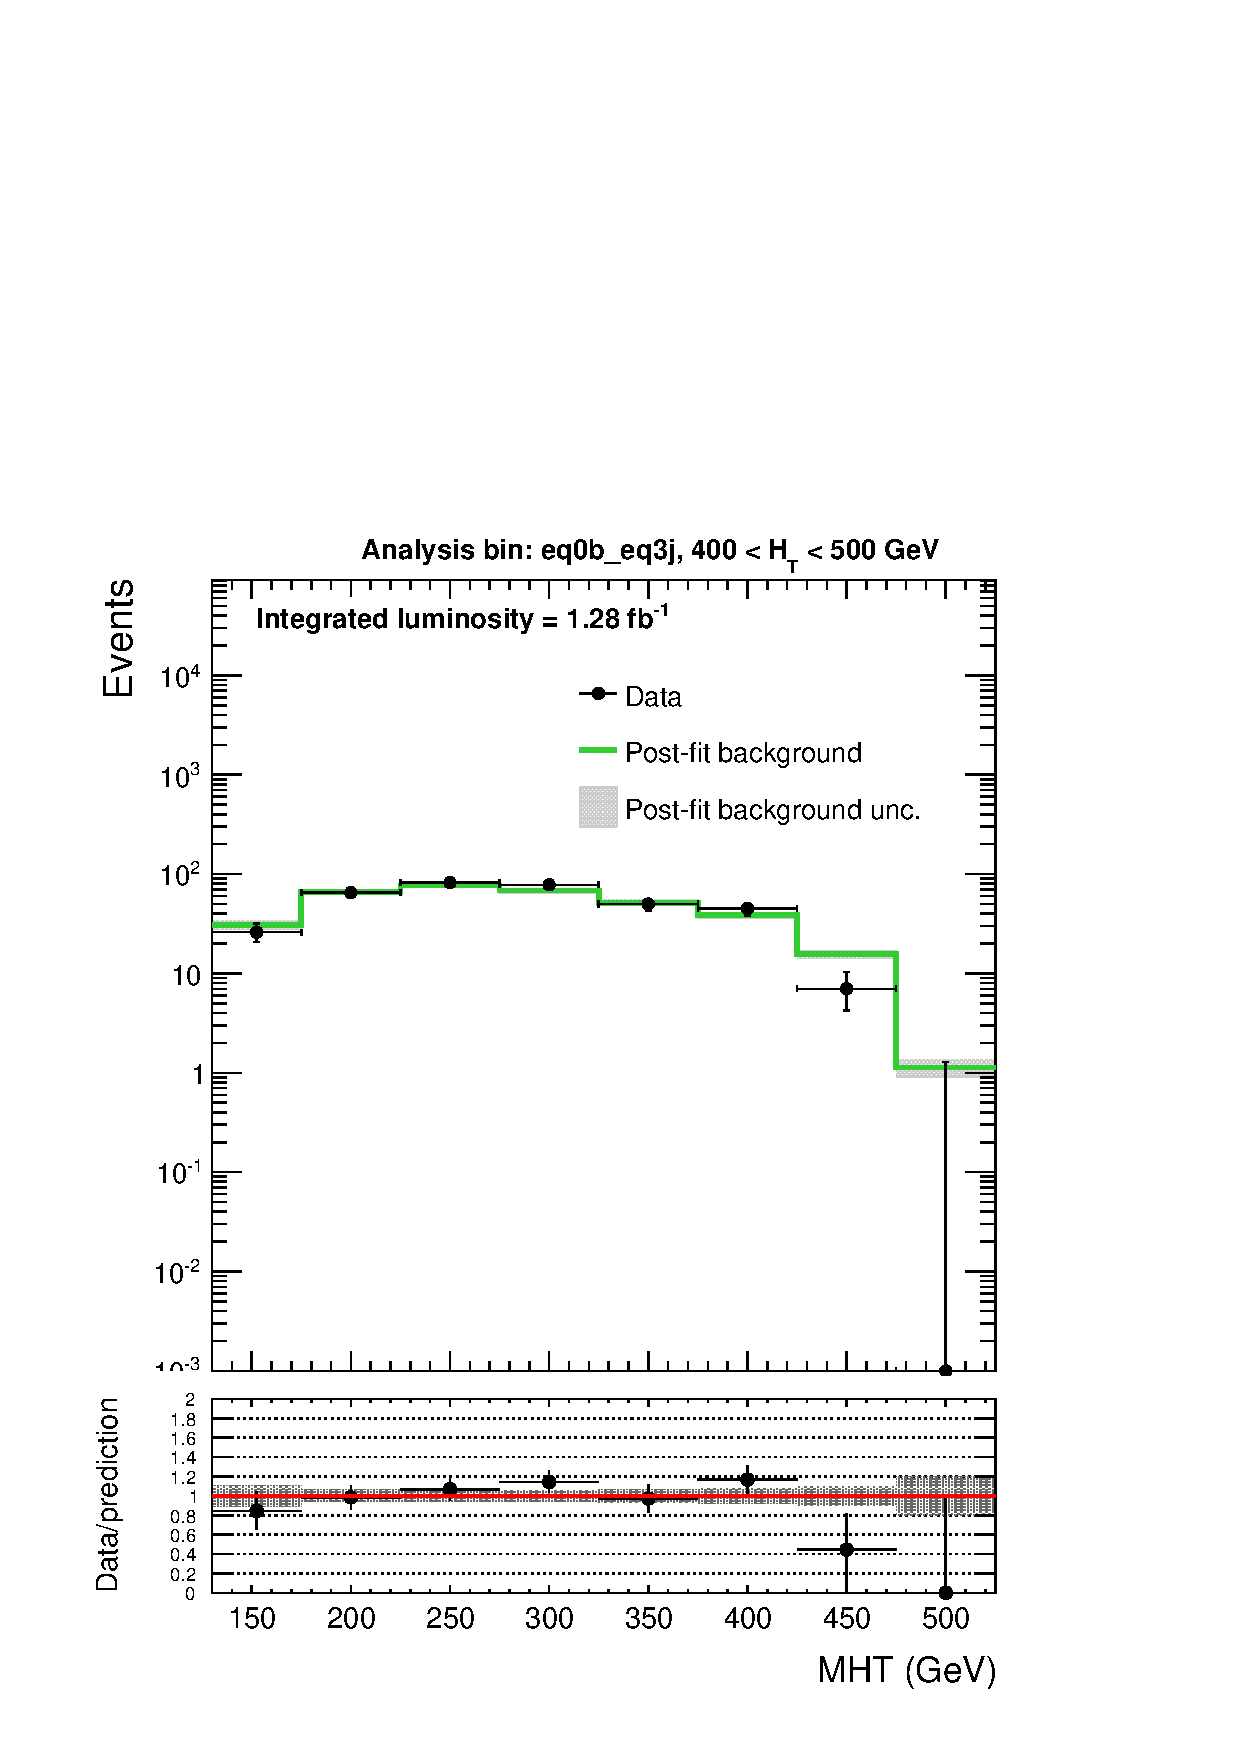
\includegraphics[width=0.25\textwidth]{figures/postFitResults/postFitShape_eq0b_eq3j_400_500.pdf} }\hspace{1cm}
    \subfigure[$\nj^{\mathrm{sym}}=3$, $\nb=0$, $500 < \scalht < 600 \; \mathrm{GeV}$]{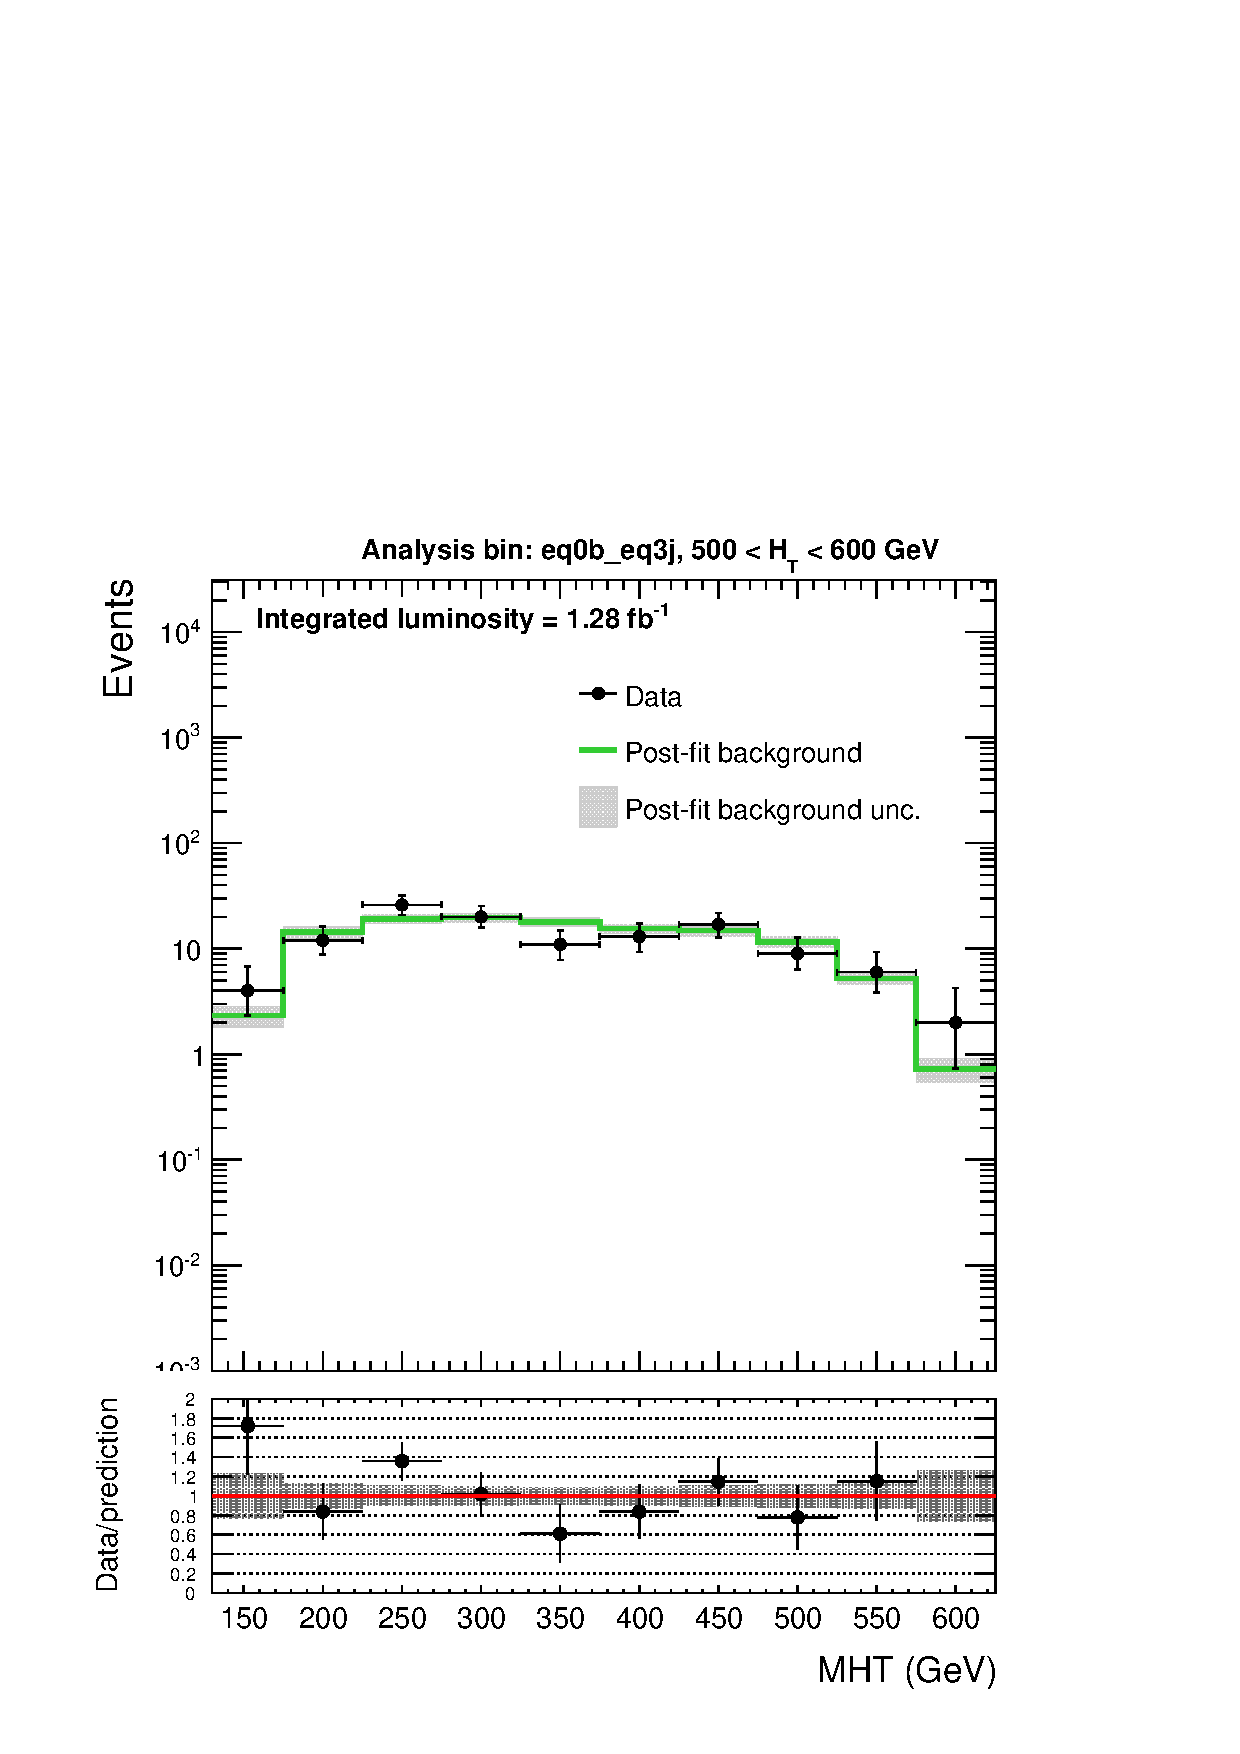
\includegraphics[width=0.25\textwidth]{figures/postFitResults/postFitShape_eq0b_eq3j_500_600.pdf} }\hspace{1cm}
    \subfigure[$\nj^{\mathrm{sym}}=3$, $\nb=0$, $600 < \scalht < 800 \; \mathrm{GeV}$]{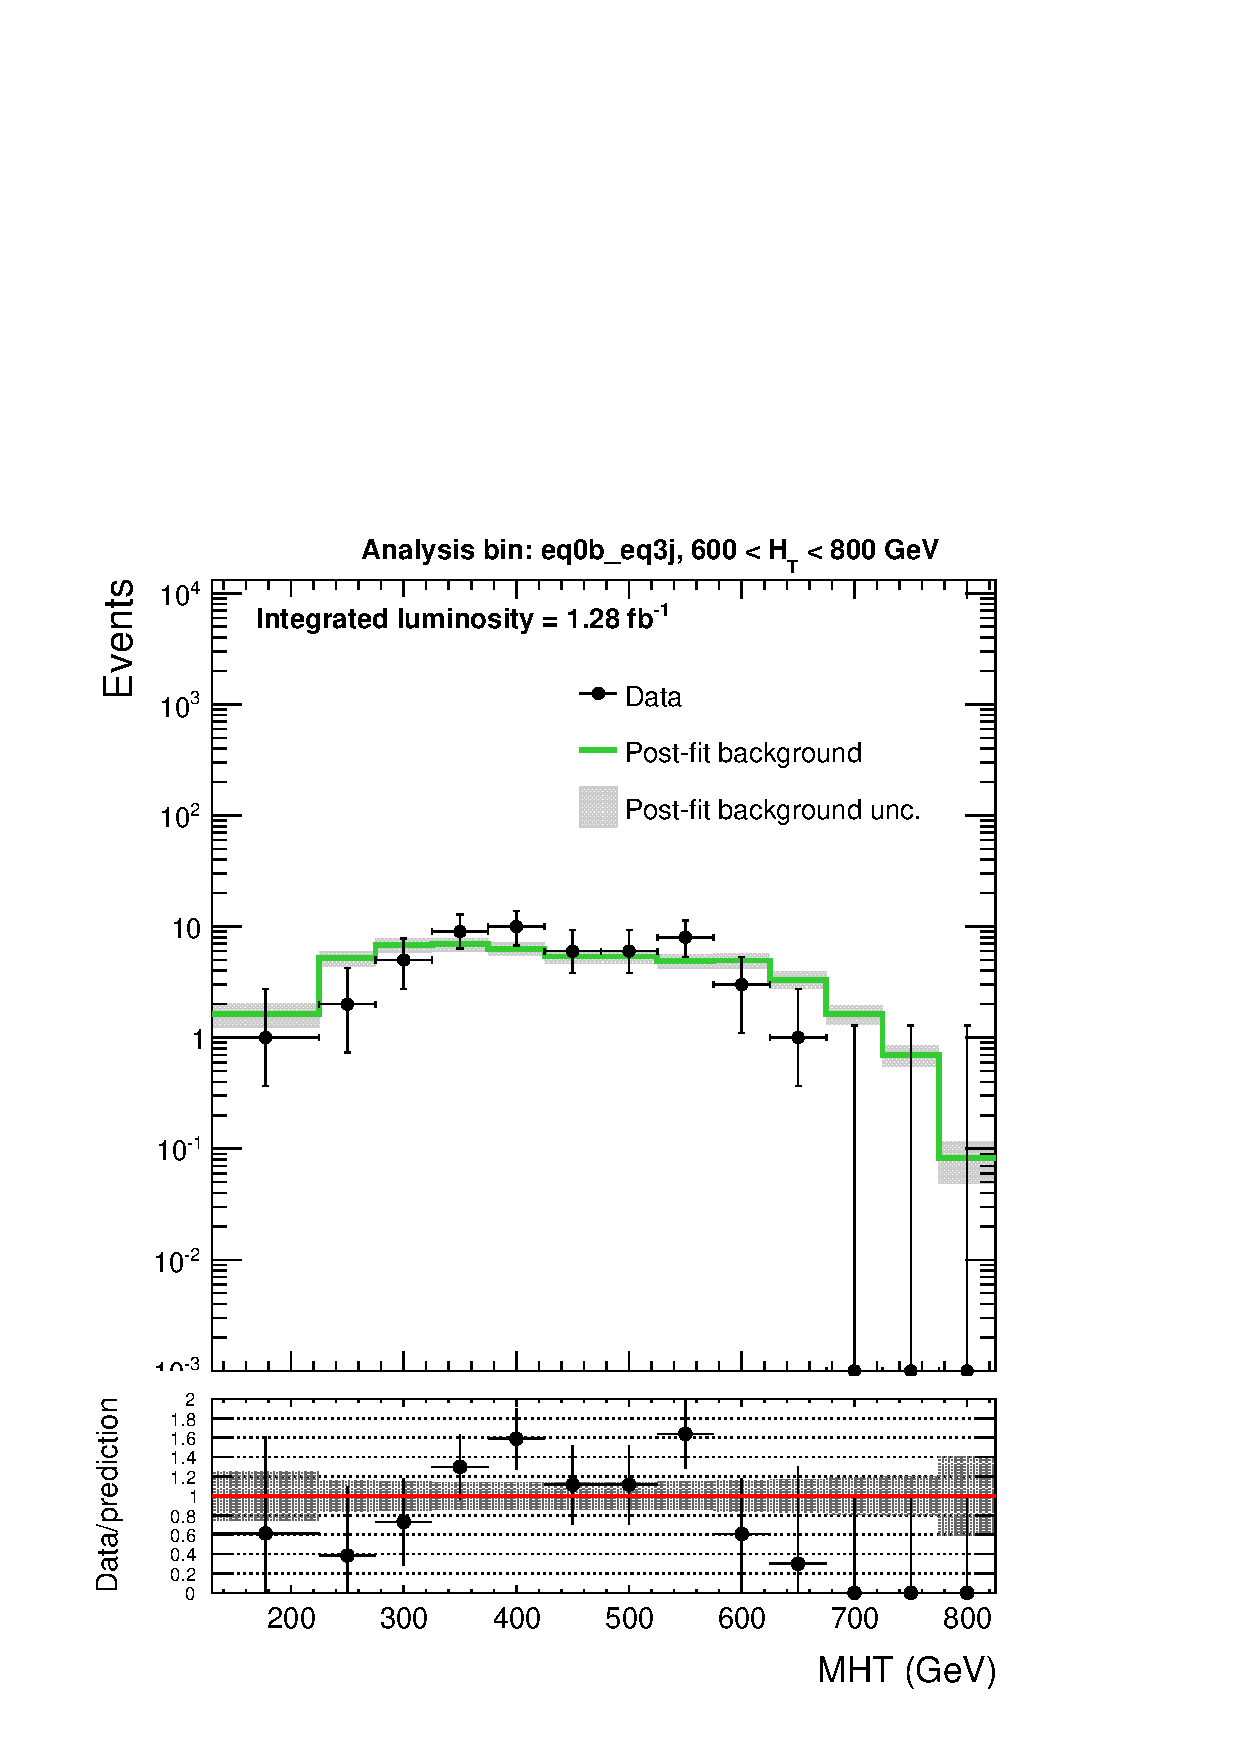
\includegraphics[width=0.25\textwidth]{figures/postFitResults/postFitShape_eq0b_eq3j_600_800.pdf} }\\
    \subfigure[$\nj^{\mathrm{sym}}=3$, $\nb=0$, $\scalht > 800 \; \mathrm{GeV}$]{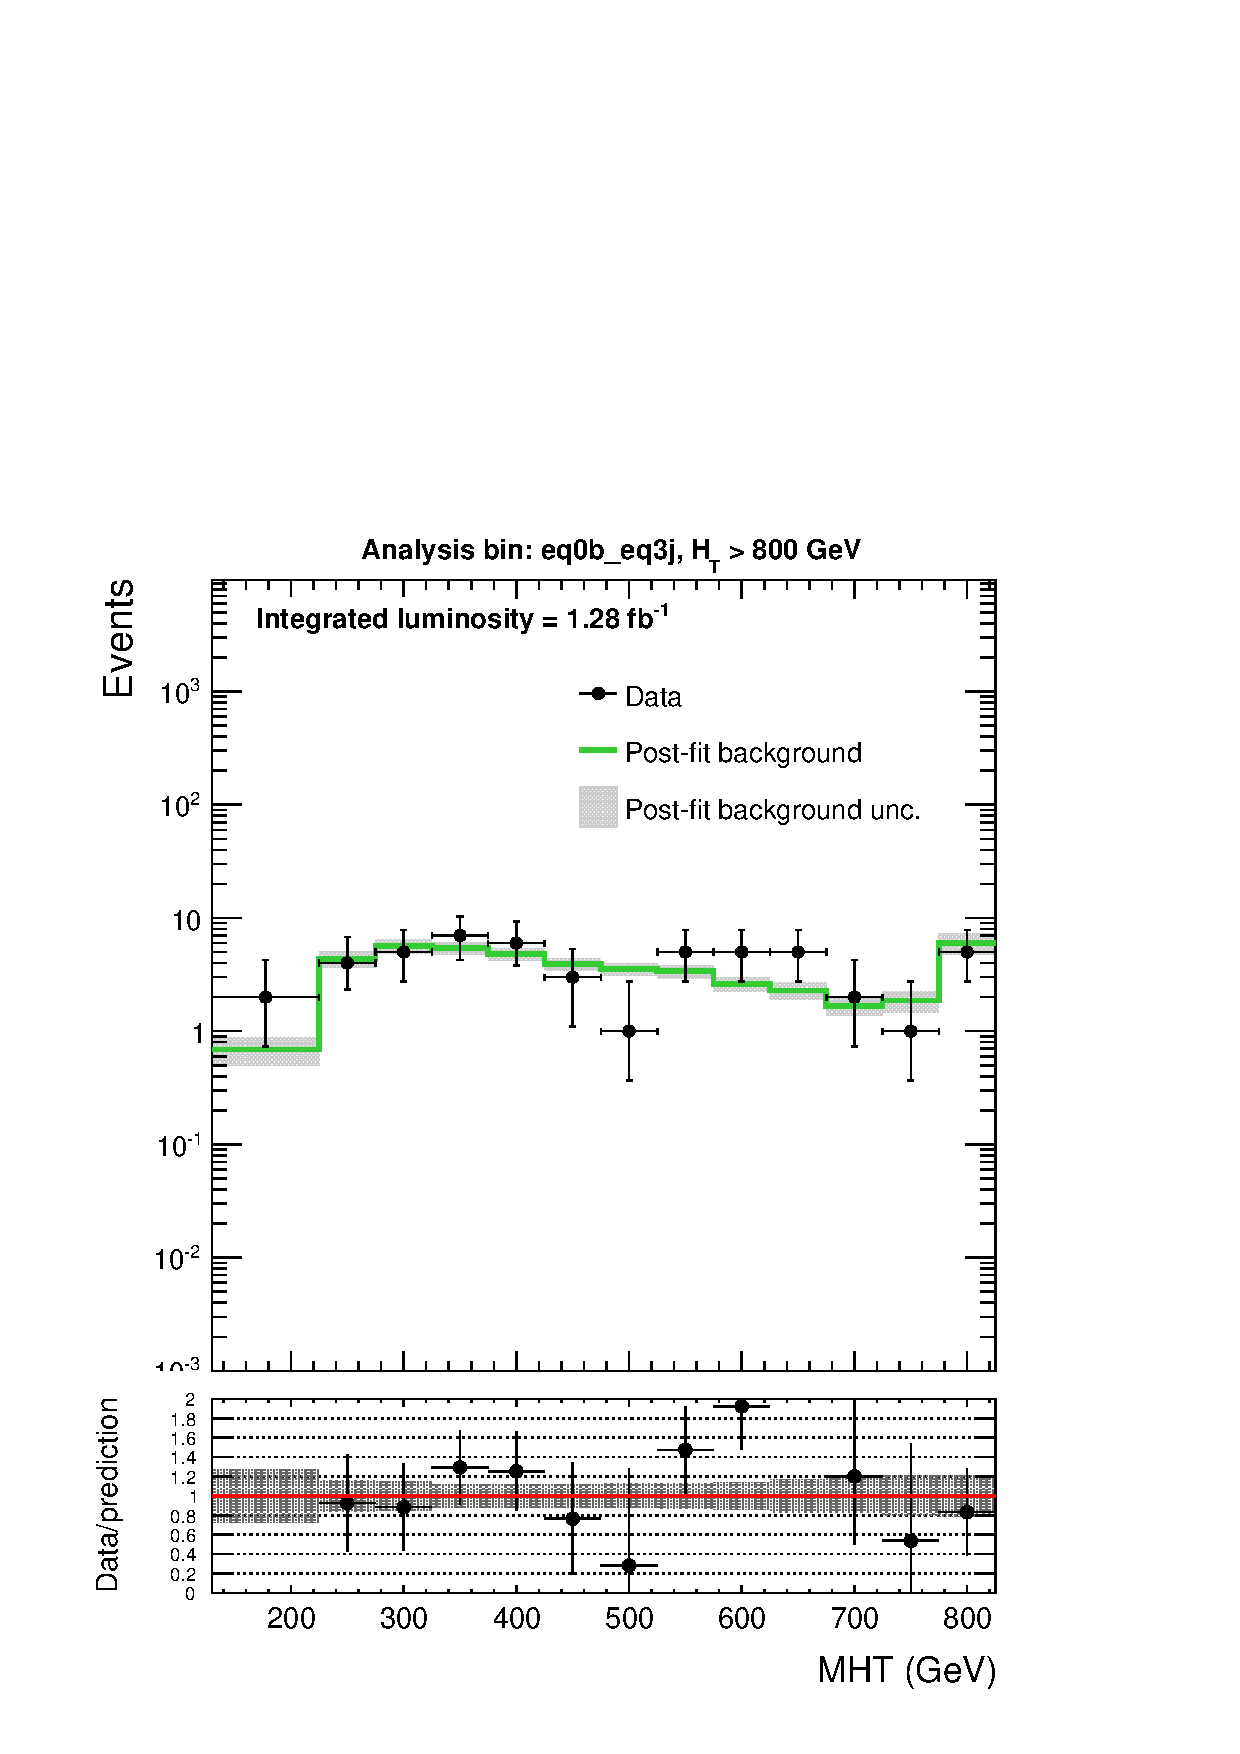
\includegraphics[width=0.25\textwidth]{figures/postFitResults/postFitShape_eq0b_eq3j_800_Inf.pdf} }\hspace{1cm}
  \end{center}
\end{figure}



\newpage
\begin{figure}[h!]
\caption{Post-fit \MHT templates for the bin $\nj^{\mathrm{asym}}=4$, $\nb=0$ \label{fig:postFitShapes_eq0b_eq4a}}.
\begin{center}

    \subfigure[$\nj^{\mathrm{asym}}=4$, $\nb=0$, $200 < \scalht < 250 \; \mathrm{GeV}$]{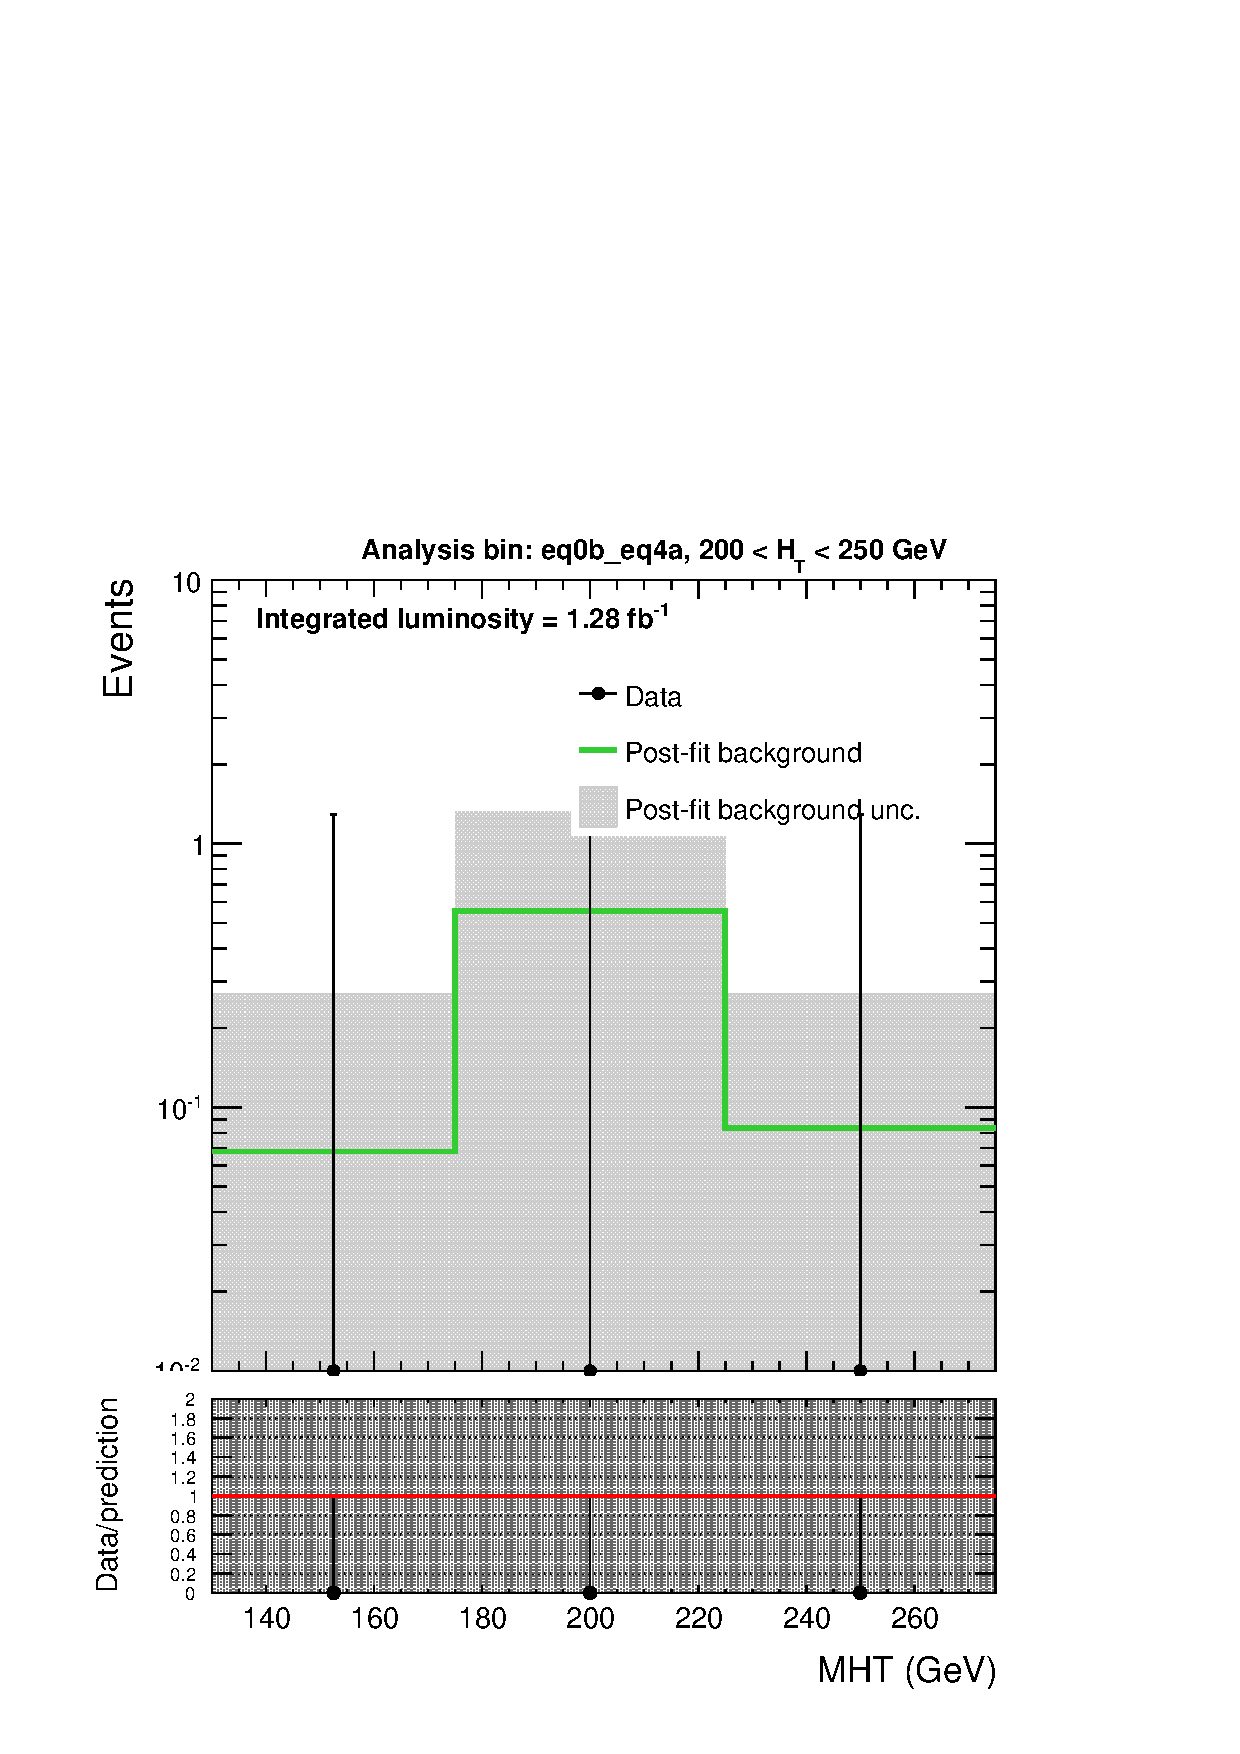
\includegraphics[width=0.25\textwidth]{figures/postFitResults/postFitShape_eq0b_eq4a_200_250.pdf} }\hspace{1cm}
    \subfigure[$\nj^{\mathrm{asym}}=4$, $\nb=0$, $250 < \scalht < 300 \; \mathrm{GeV}$]{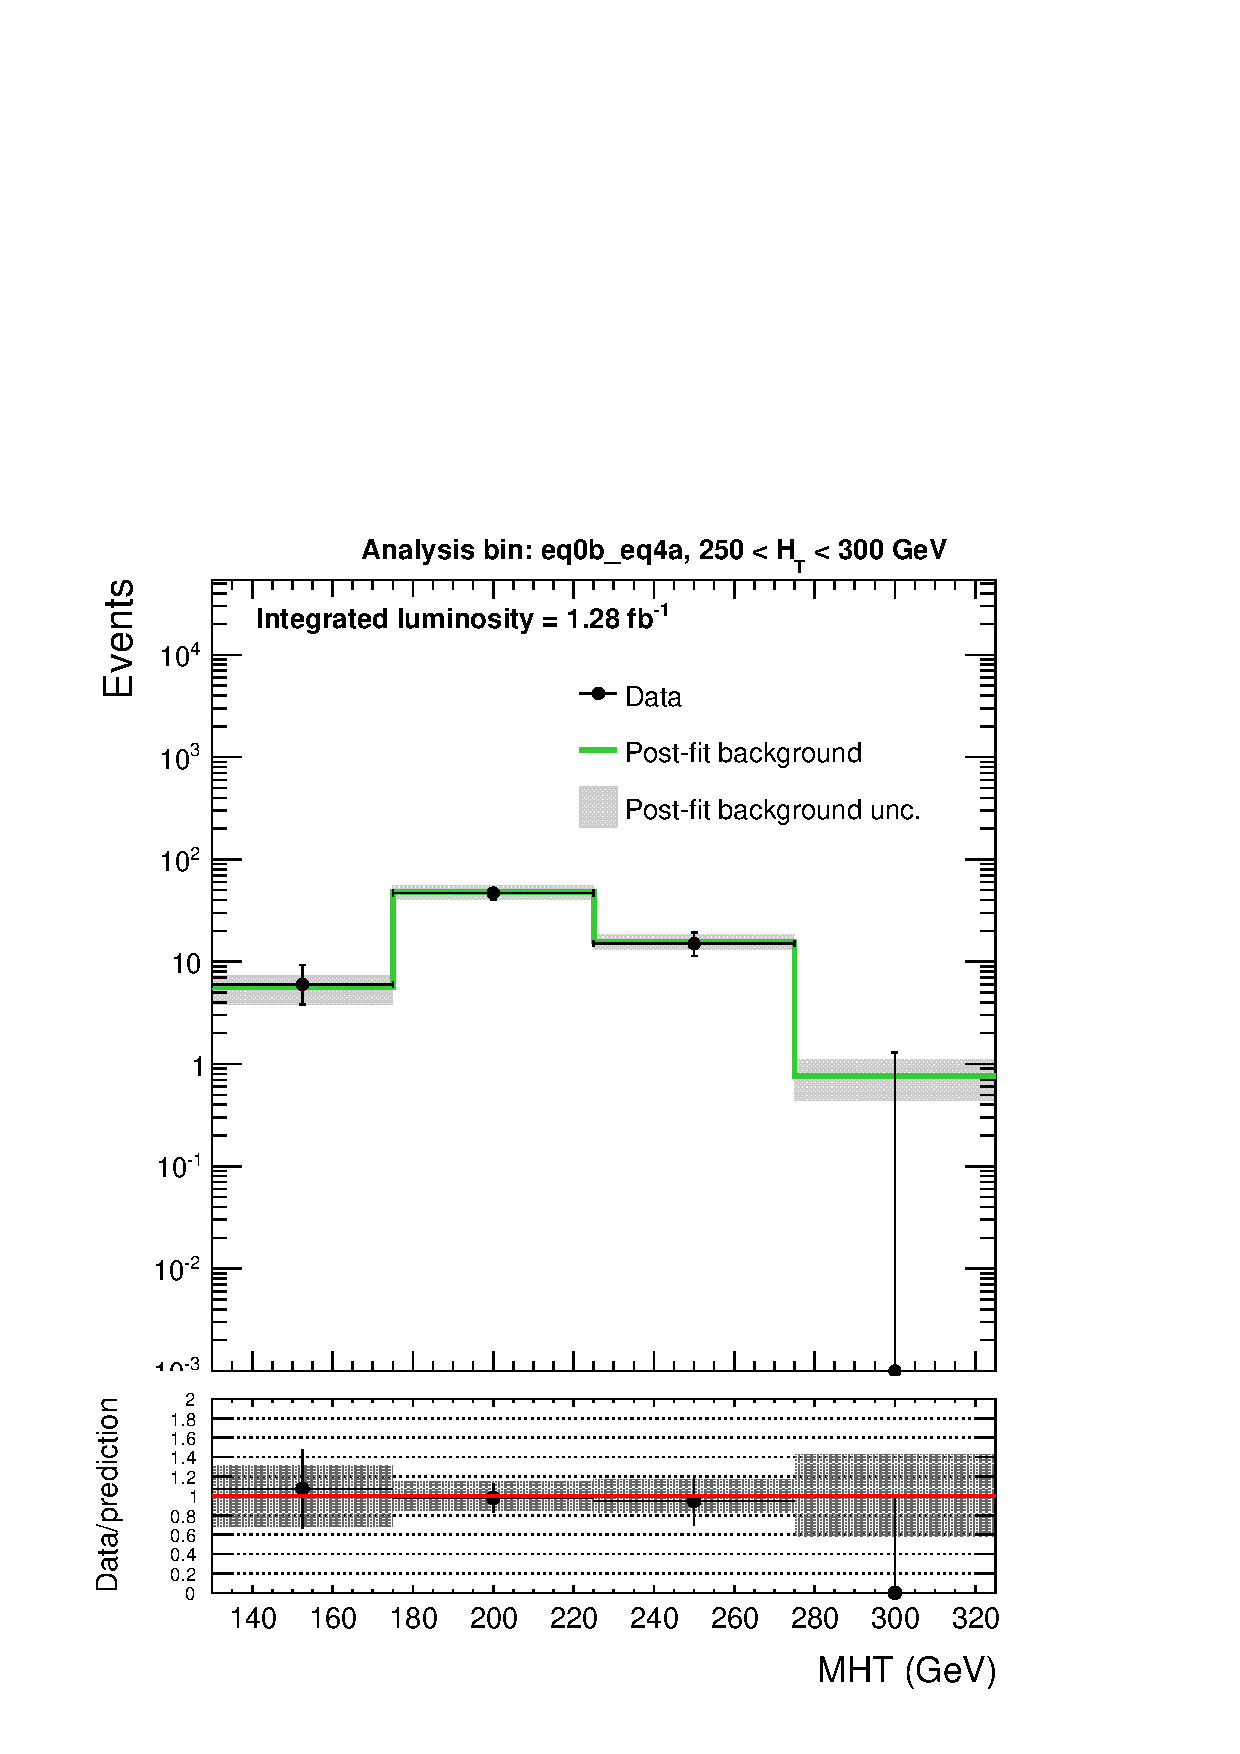
\includegraphics[width=0.25\textwidth]{figures/postFitResults/postFitShape_eq0b_eq4a_250_300.pdf} }\hspace{1cm}
    \subfigure[$\nj^{\mathrm{asym}}=4$, $\nb=0$, $300 < \scalht < 350 \; \mathrm{GeV}$]{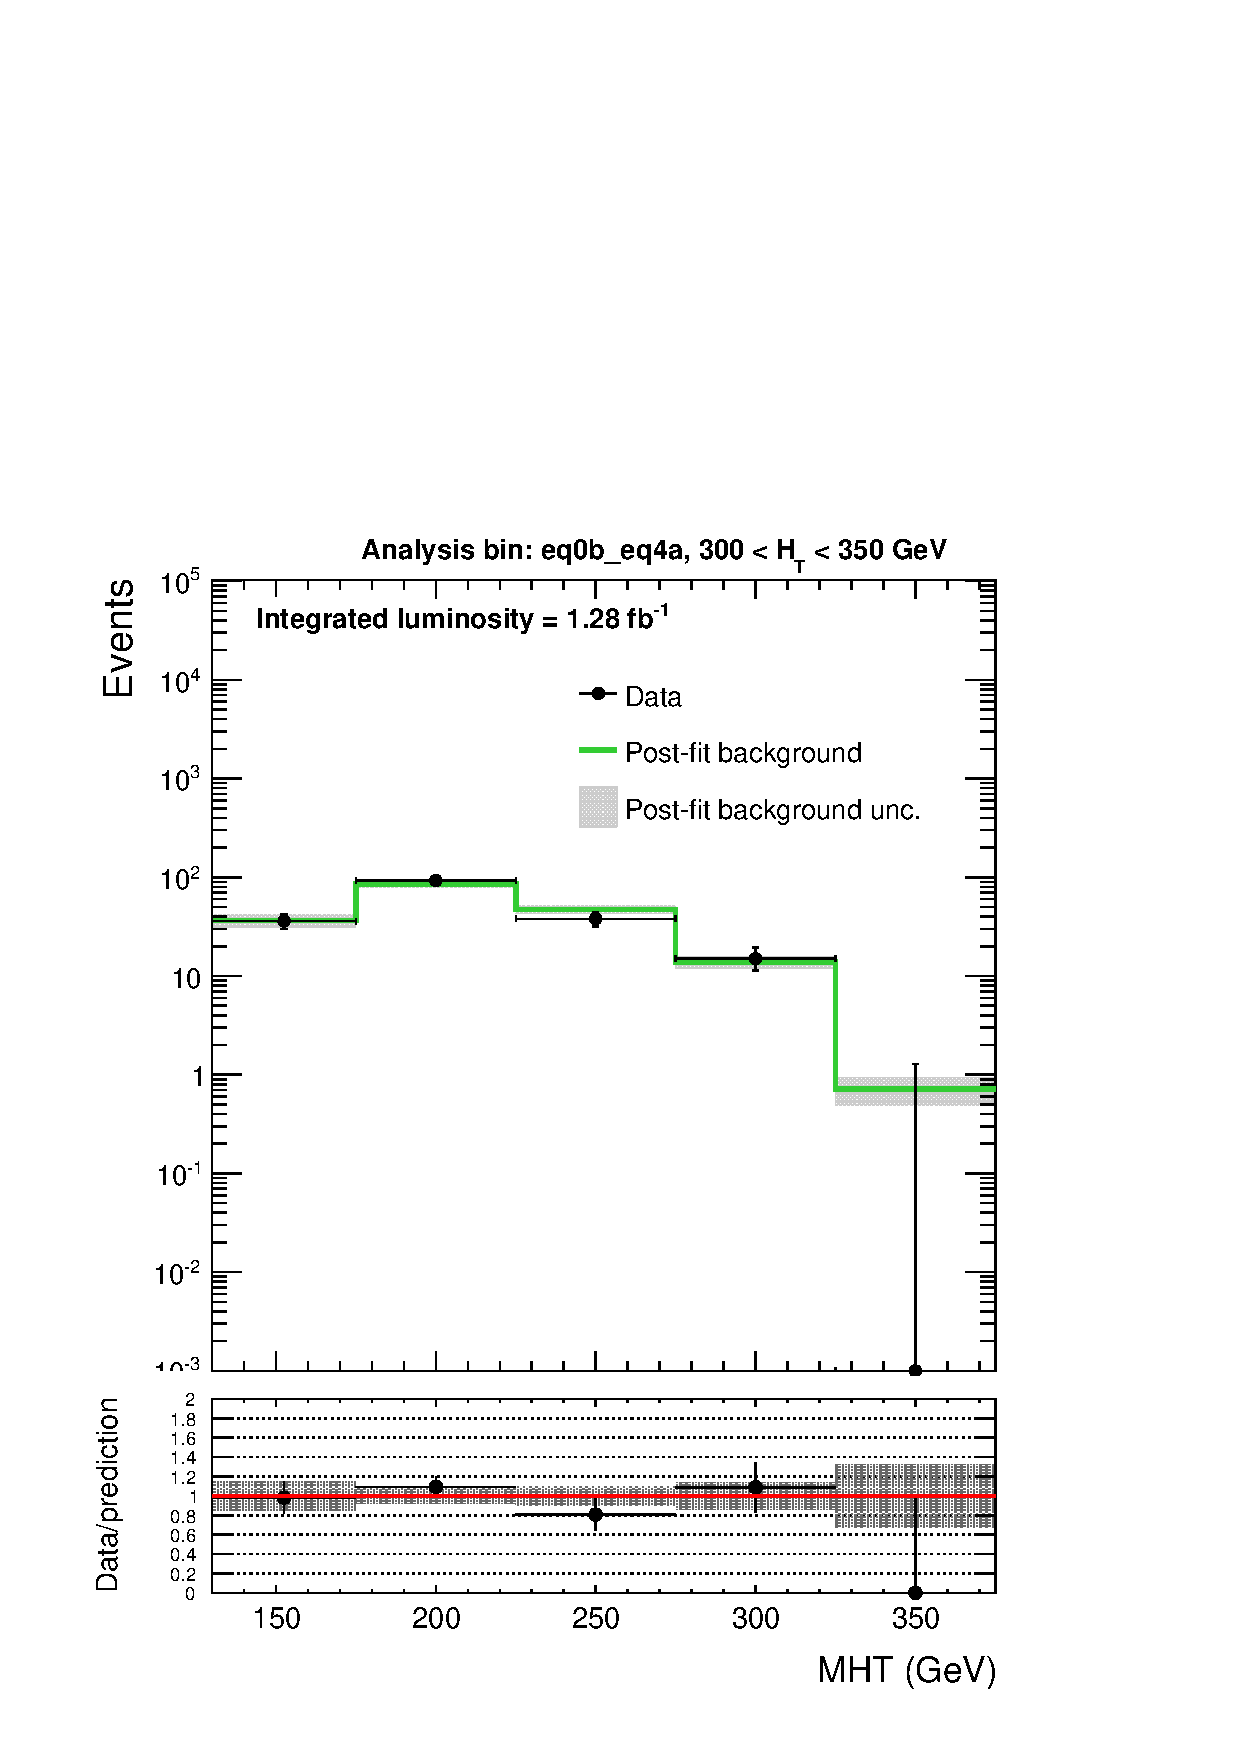
\includegraphics[width=0.25\textwidth]{figures/postFitResults/postFitShape_eq0b_eq4a_300_350.pdf} }\\
    \subfigure[$\nj^{\mathrm{asym}}=4$, $\nb=0$, $350 < \scalht < 400 \; \mathrm{GeV}$]{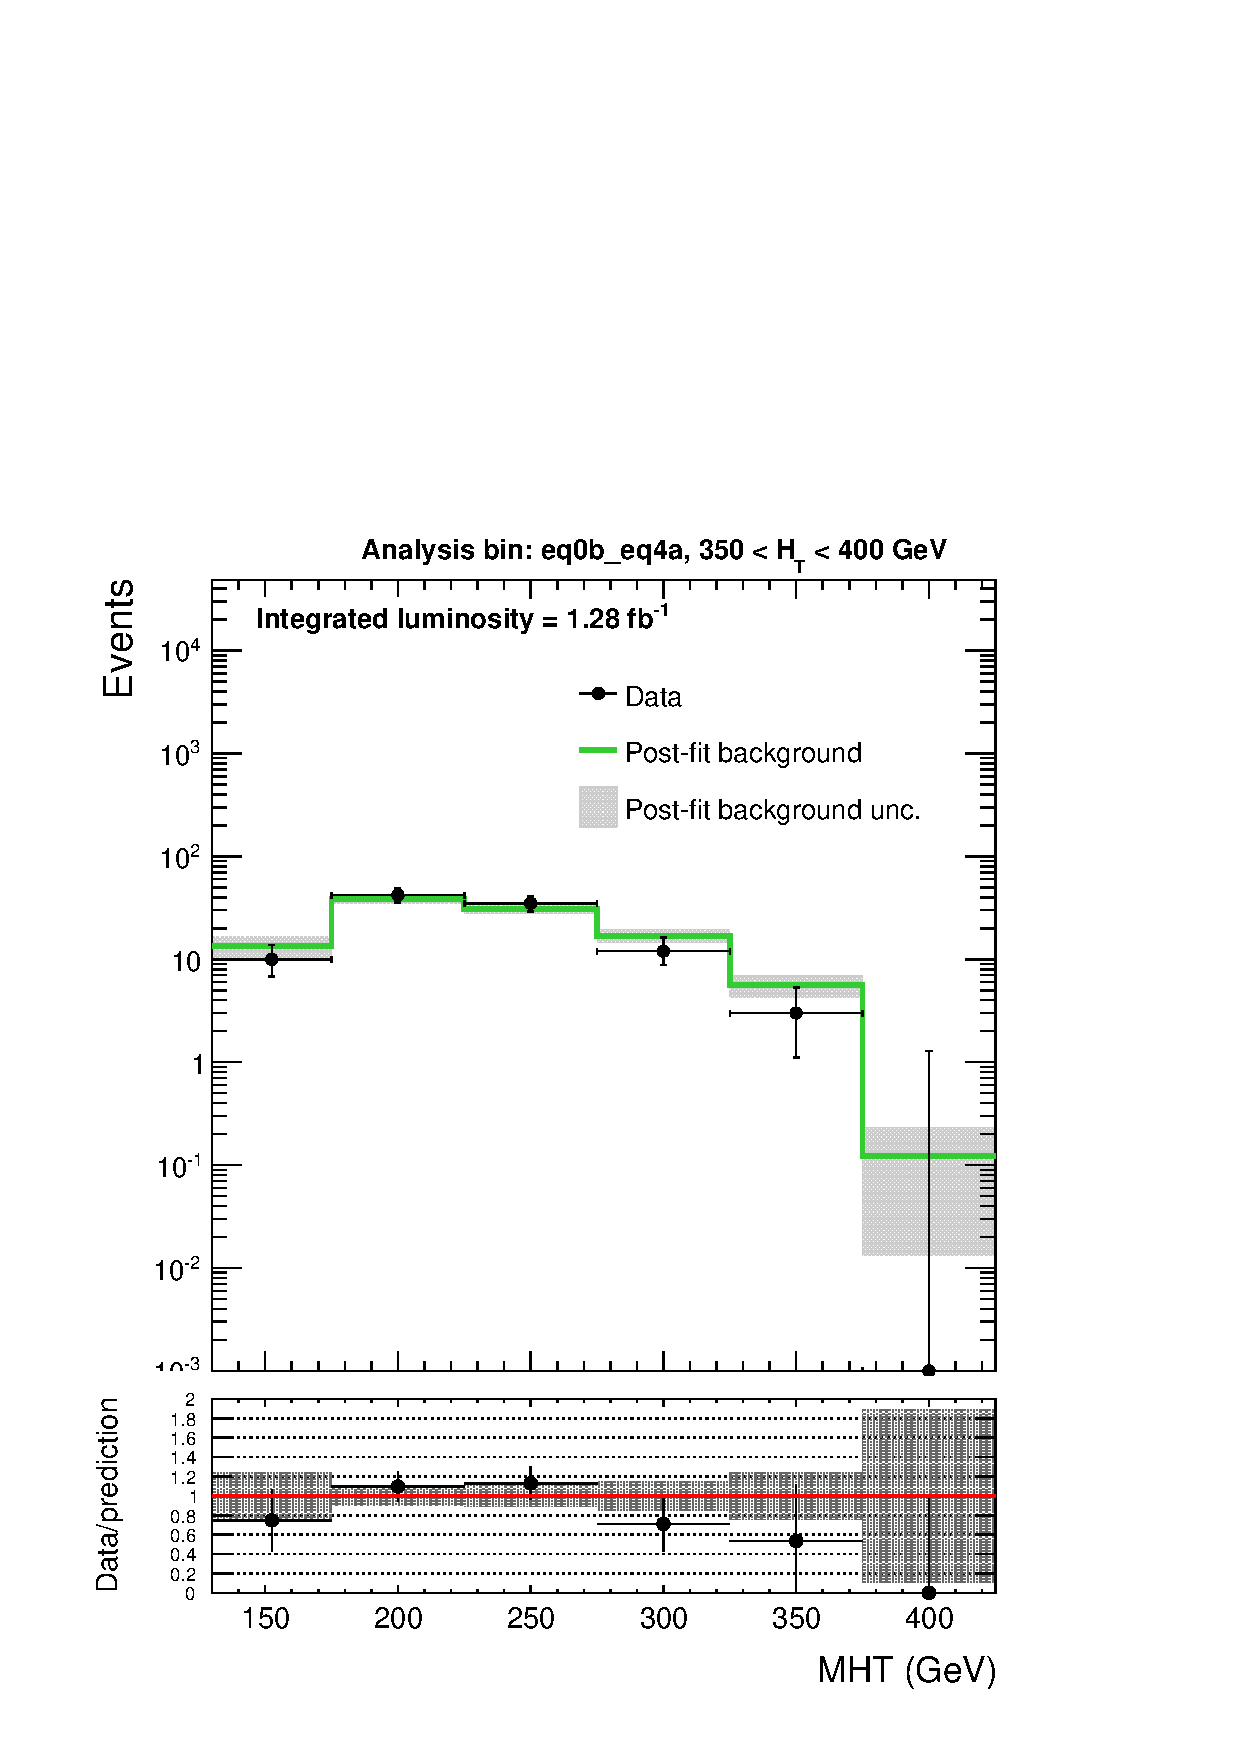
\includegraphics[width=0.25\textwidth]{figures/postFitResults/postFitShape_eq0b_eq4a_350_400.pdf} }\hspace{1cm}
    \subfigure[$\nj^{\mathrm{asym}}=4$, $\nb=0$, $400 < \scalht < 500 \; \mathrm{GeV}$]{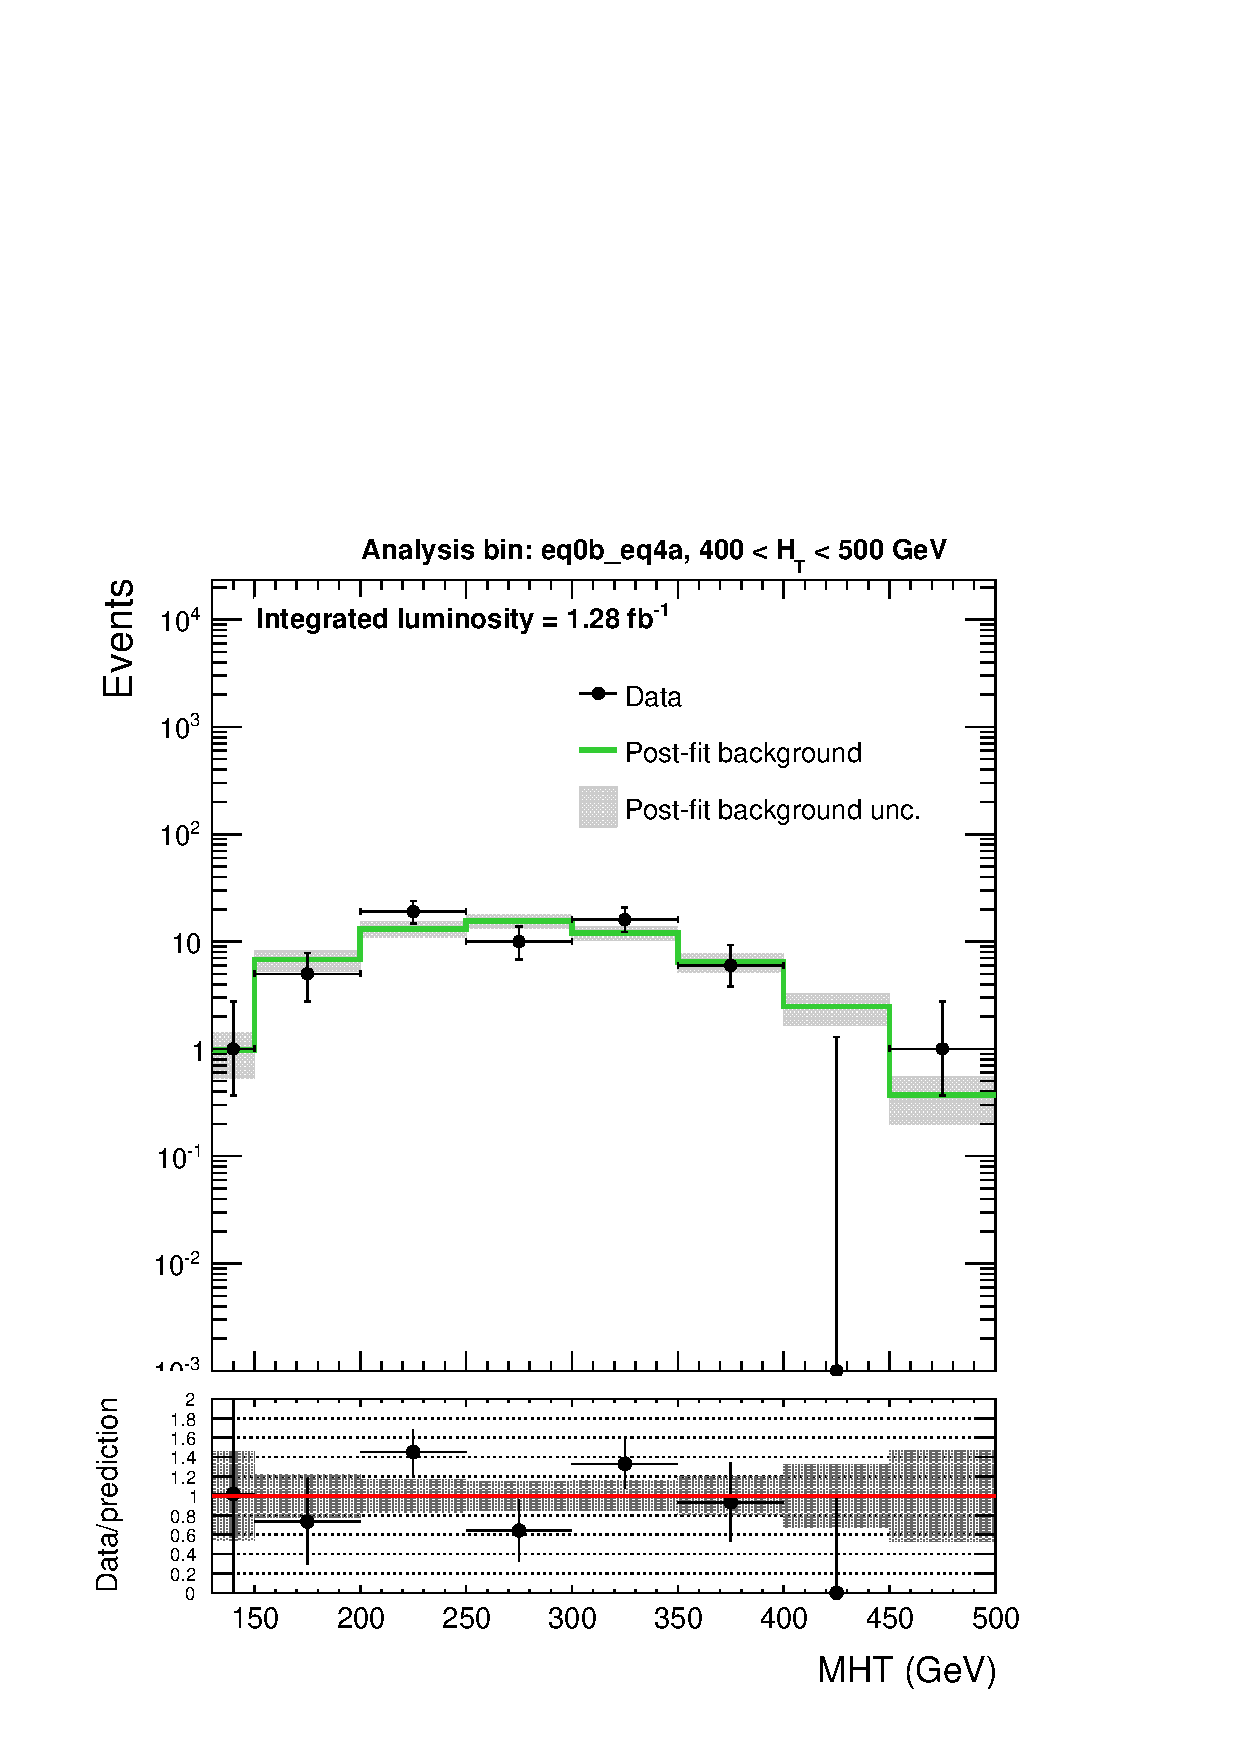
\includegraphics[width=0.25\textwidth]{figures/postFitResults/postFitShape_eq0b_eq4a_400_500.pdf} }\hspace{1cm}
    \subfigure[$\nj^{\mathrm{asym}}=4$, $\nb=0$, $500 < \scalht < 600 \; \mathrm{GeV}$]{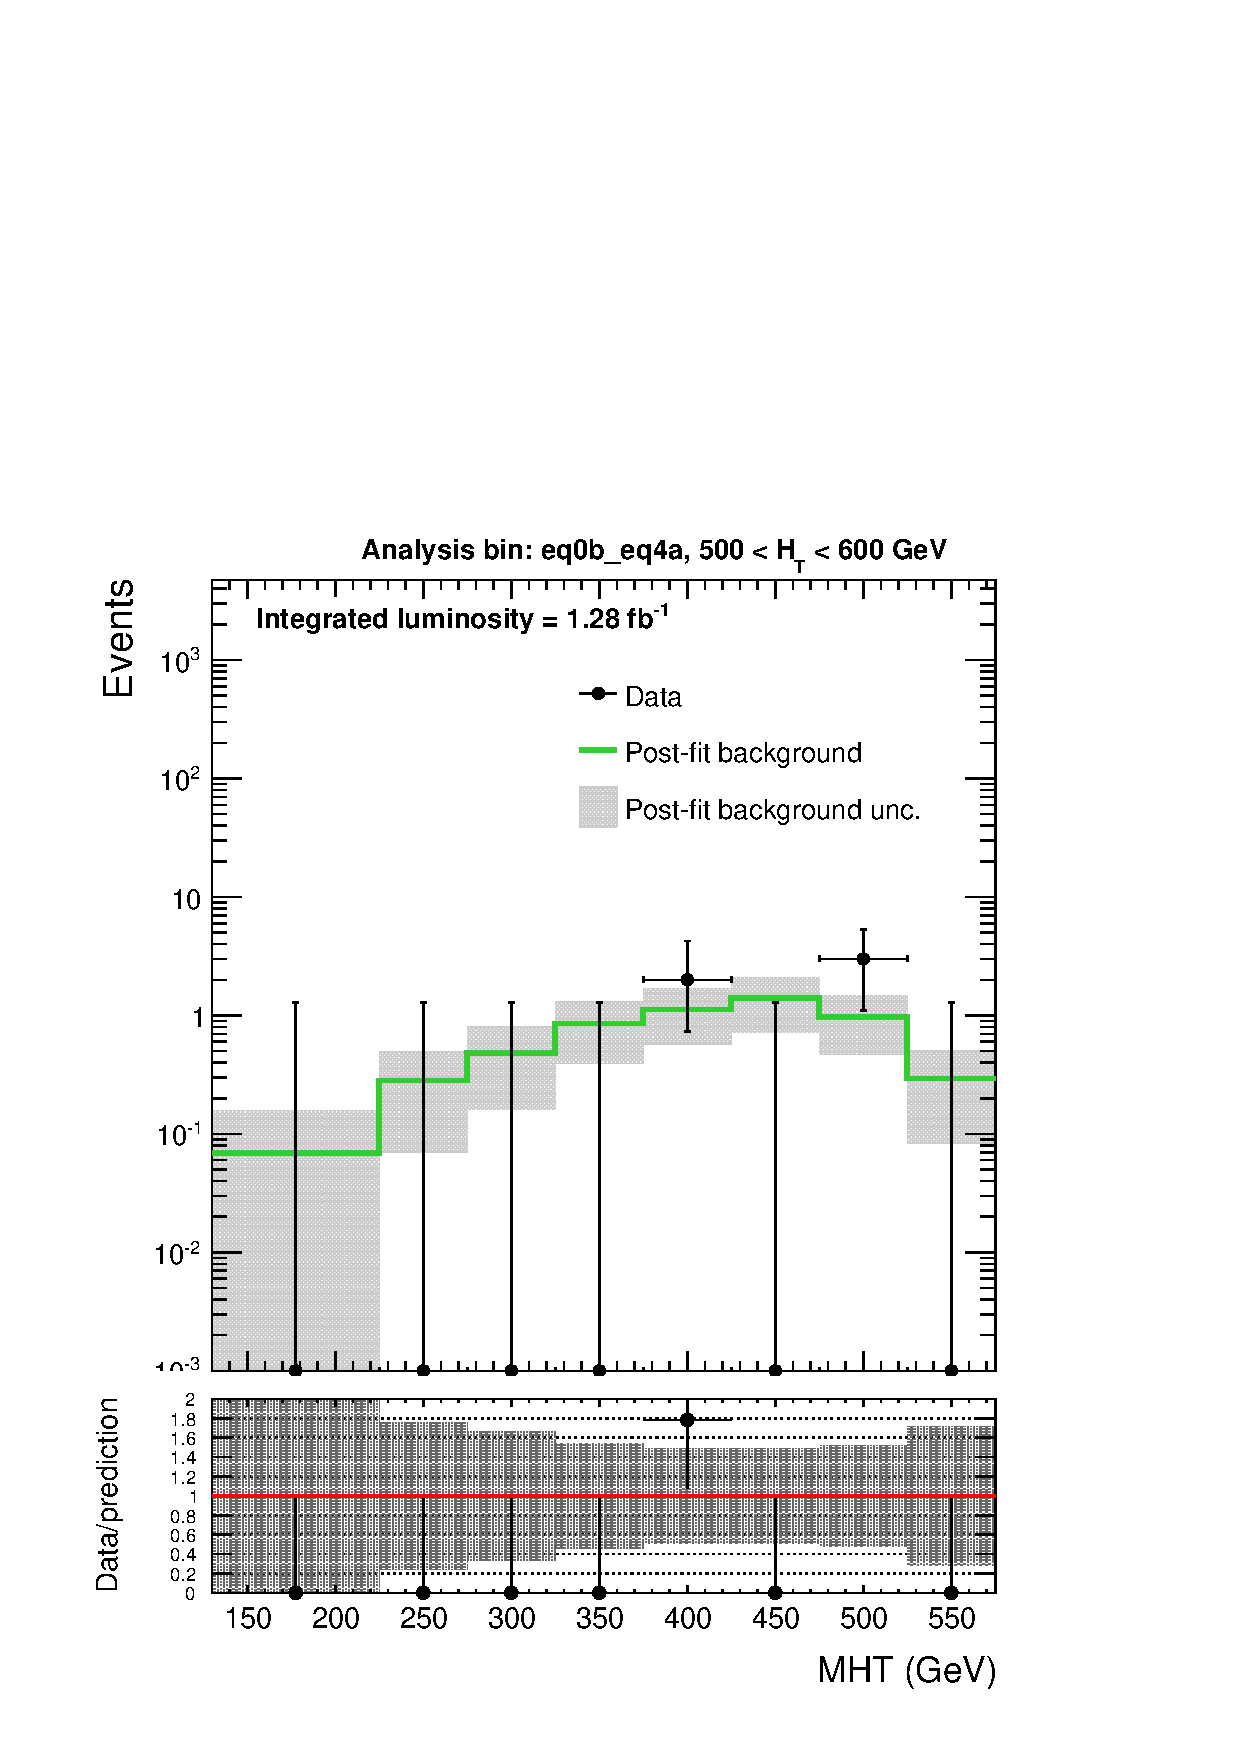
\includegraphics[width=0.25\textwidth]{figures/postFitResults/postFitShape_eq0b_eq4a_500_600.pdf} }\\
    \subfigure[$\nj^{\mathrm{asym}}=4$, $\nb=0$, $\scalht > 600 \; \mathrm{GeV}$]{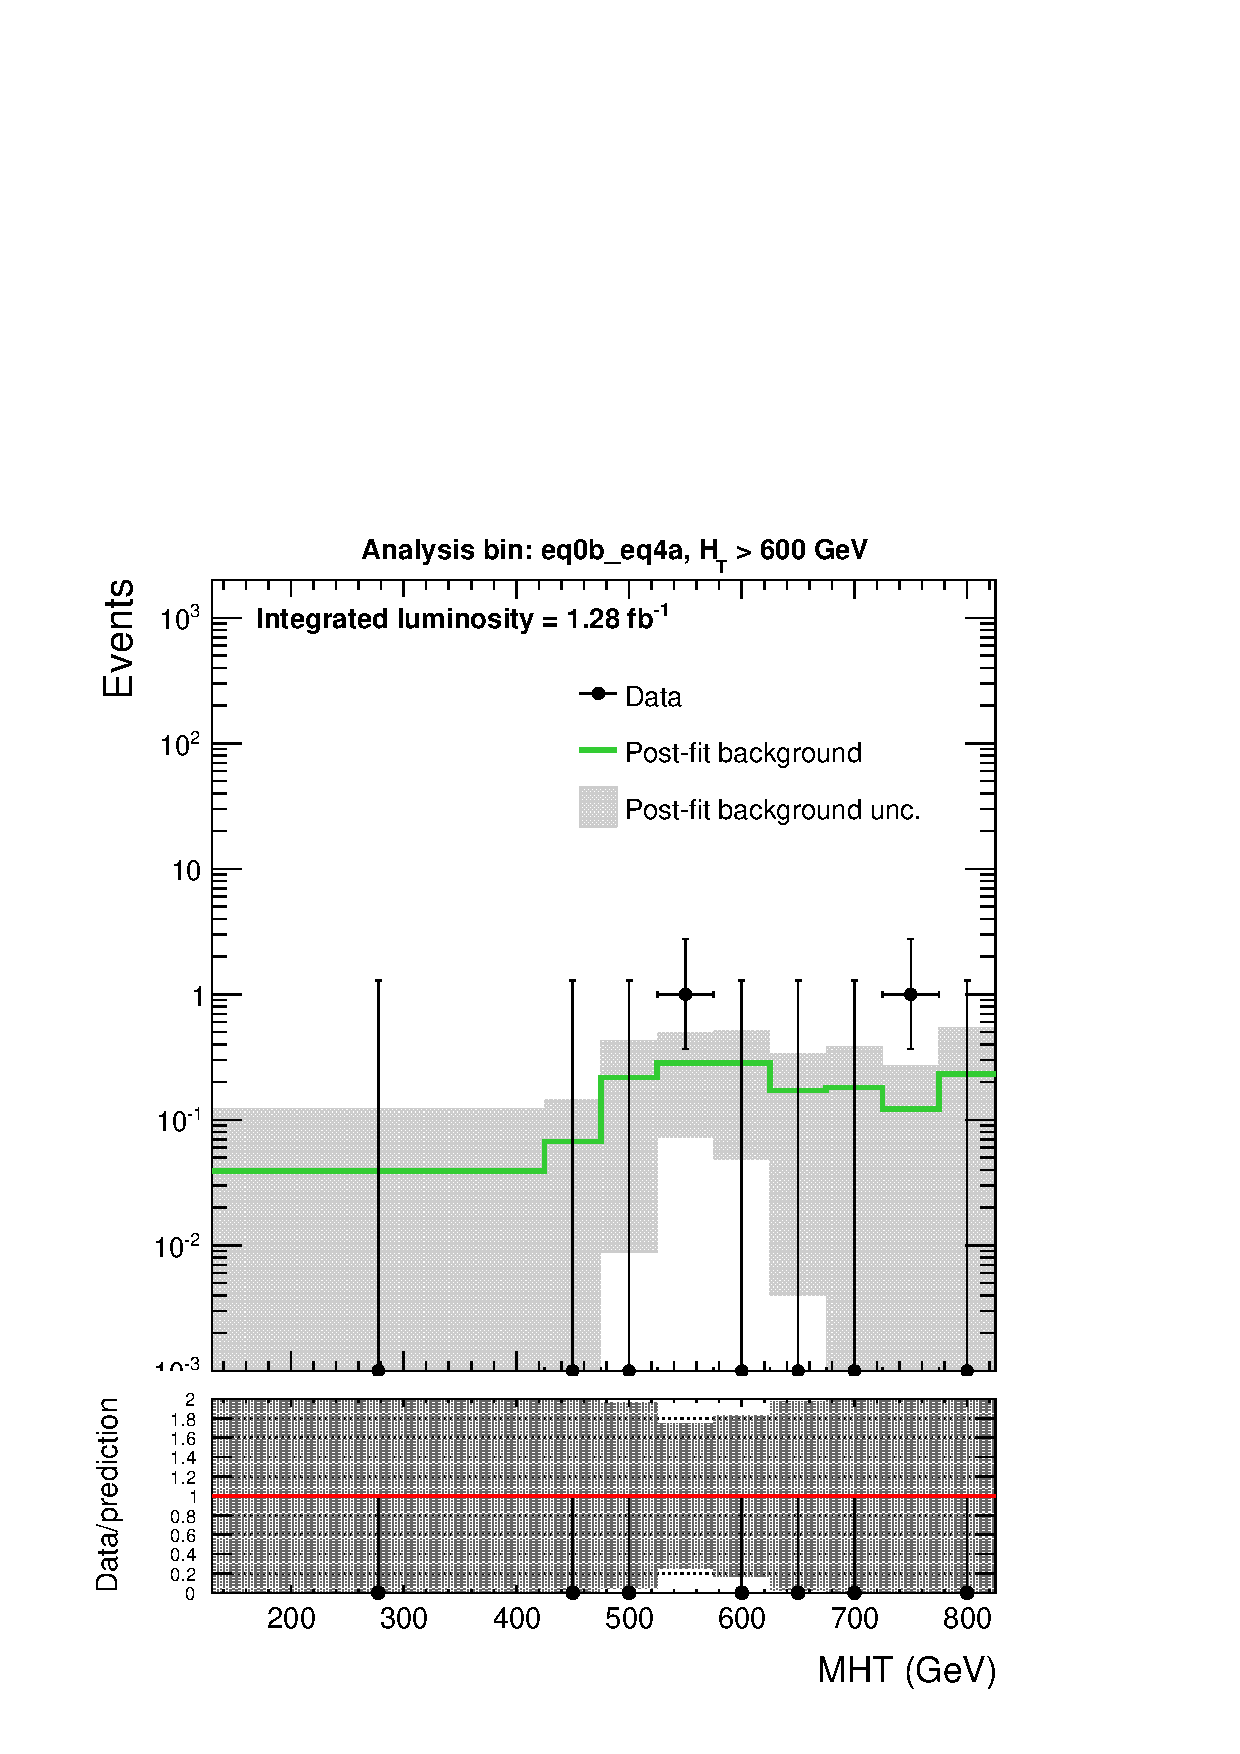
\includegraphics[width=0.25\textwidth]{figures/postFitResults/postFitShape_eq0b_eq4a_600_Inf.pdf} }\hspace{1cm}
  \end{center}
\end{figure}



\newpage
\begin{figure}[h!]
\caption{Post-fit \MHT templates for the bin $\nj^{\mathrm{sym}}=4$, $\nb=0$ \label{fig:postFitShapes_eq0b_eq4j}}.
\begin{center}

    \subfigure[$\nj^{\mathrm{sym}}=4$, $\nb=0$, $300 < \scalht < 350 \; \mathrm{GeV}$]{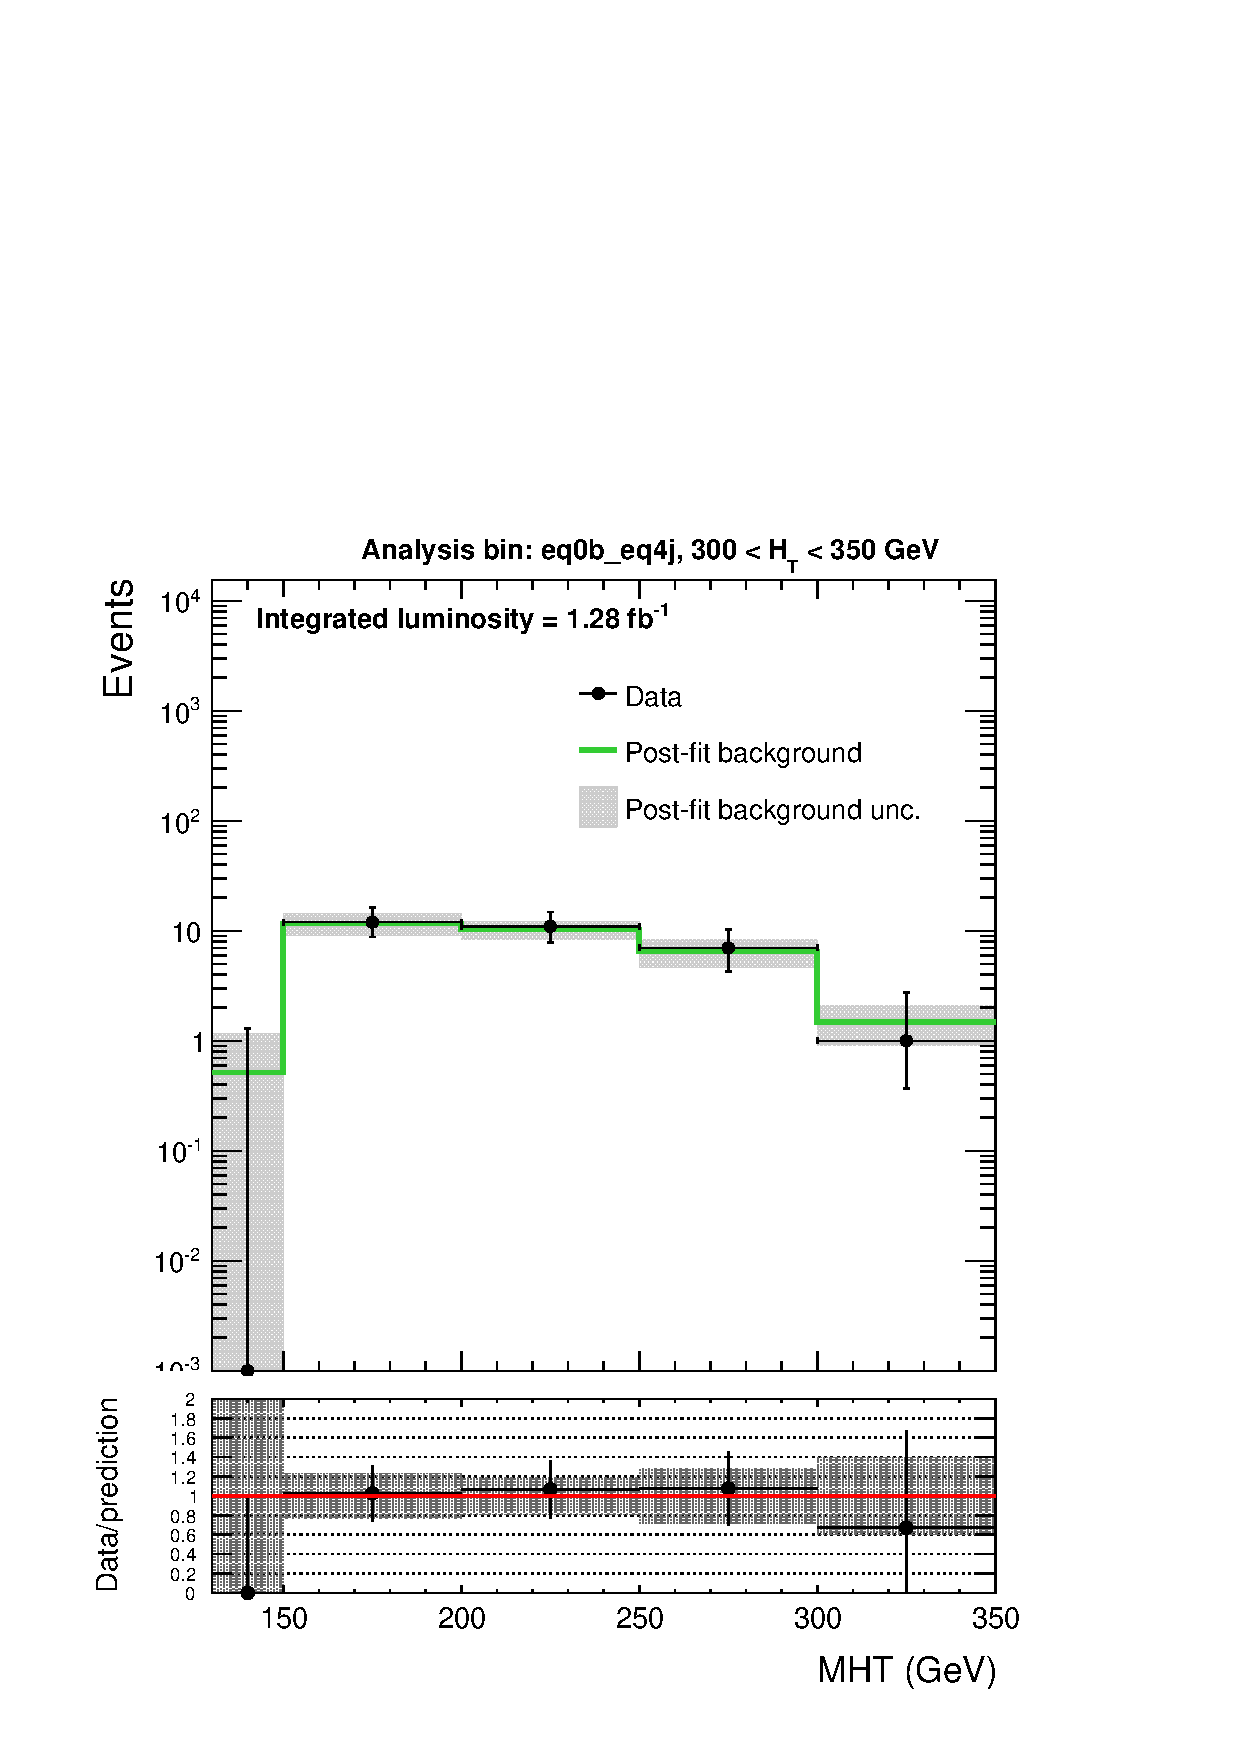
\includegraphics[width=0.25\textwidth]{figures/postFitResults/postFitShape_eq0b_eq4j_300_350.pdf} }\hspace{1cm}
    \subfigure[$\nj^{\mathrm{sym}}=4$, $\nb=0$, $350 < \scalht < 400 \; \mathrm{GeV}$]{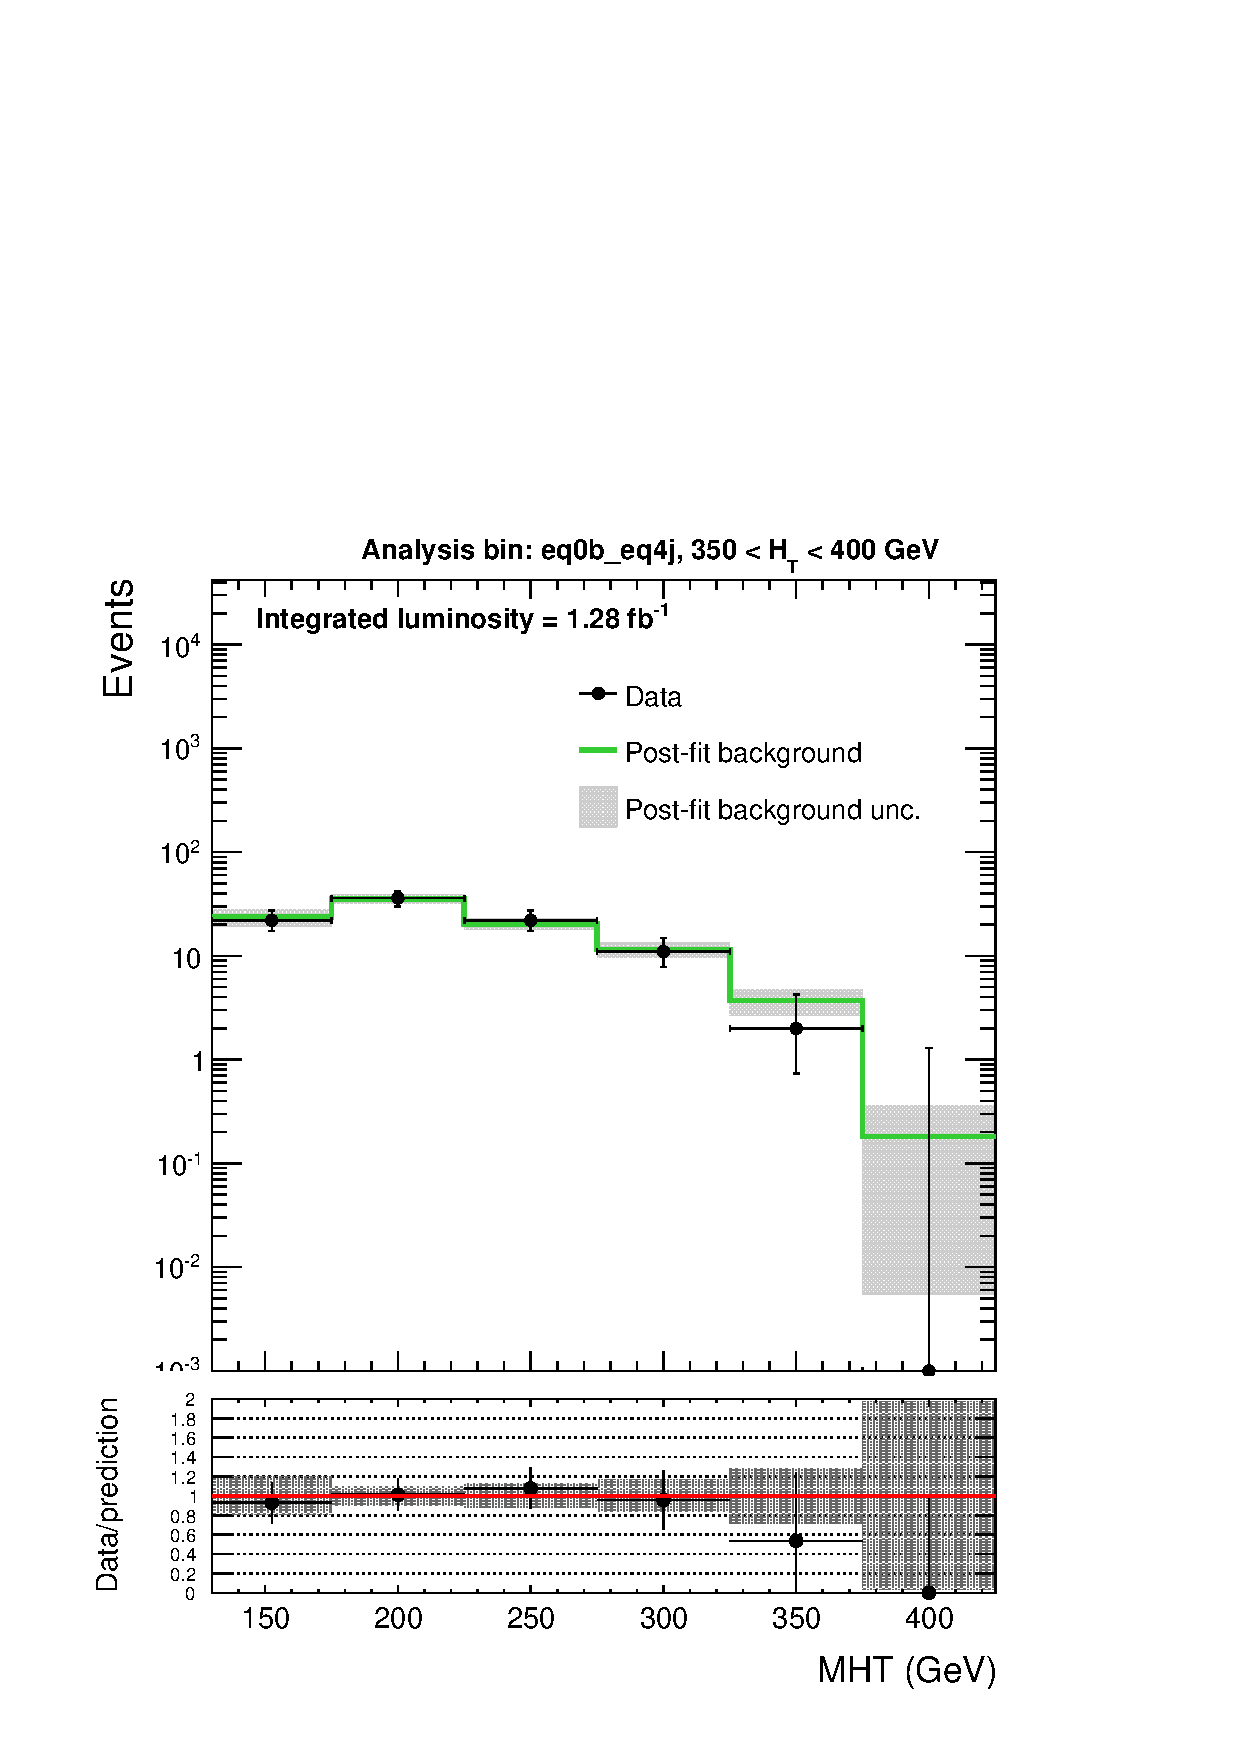
\includegraphics[width=0.25\textwidth]{figures/postFitResults/postFitShape_eq0b_eq4j_350_400.pdf} }\hspace{1cm}
    \subfigure[$\nj^{\mathrm{sym}}=4$, $\nb=0$, $400 < \scalht < 500 \; \mathrm{GeV}$]{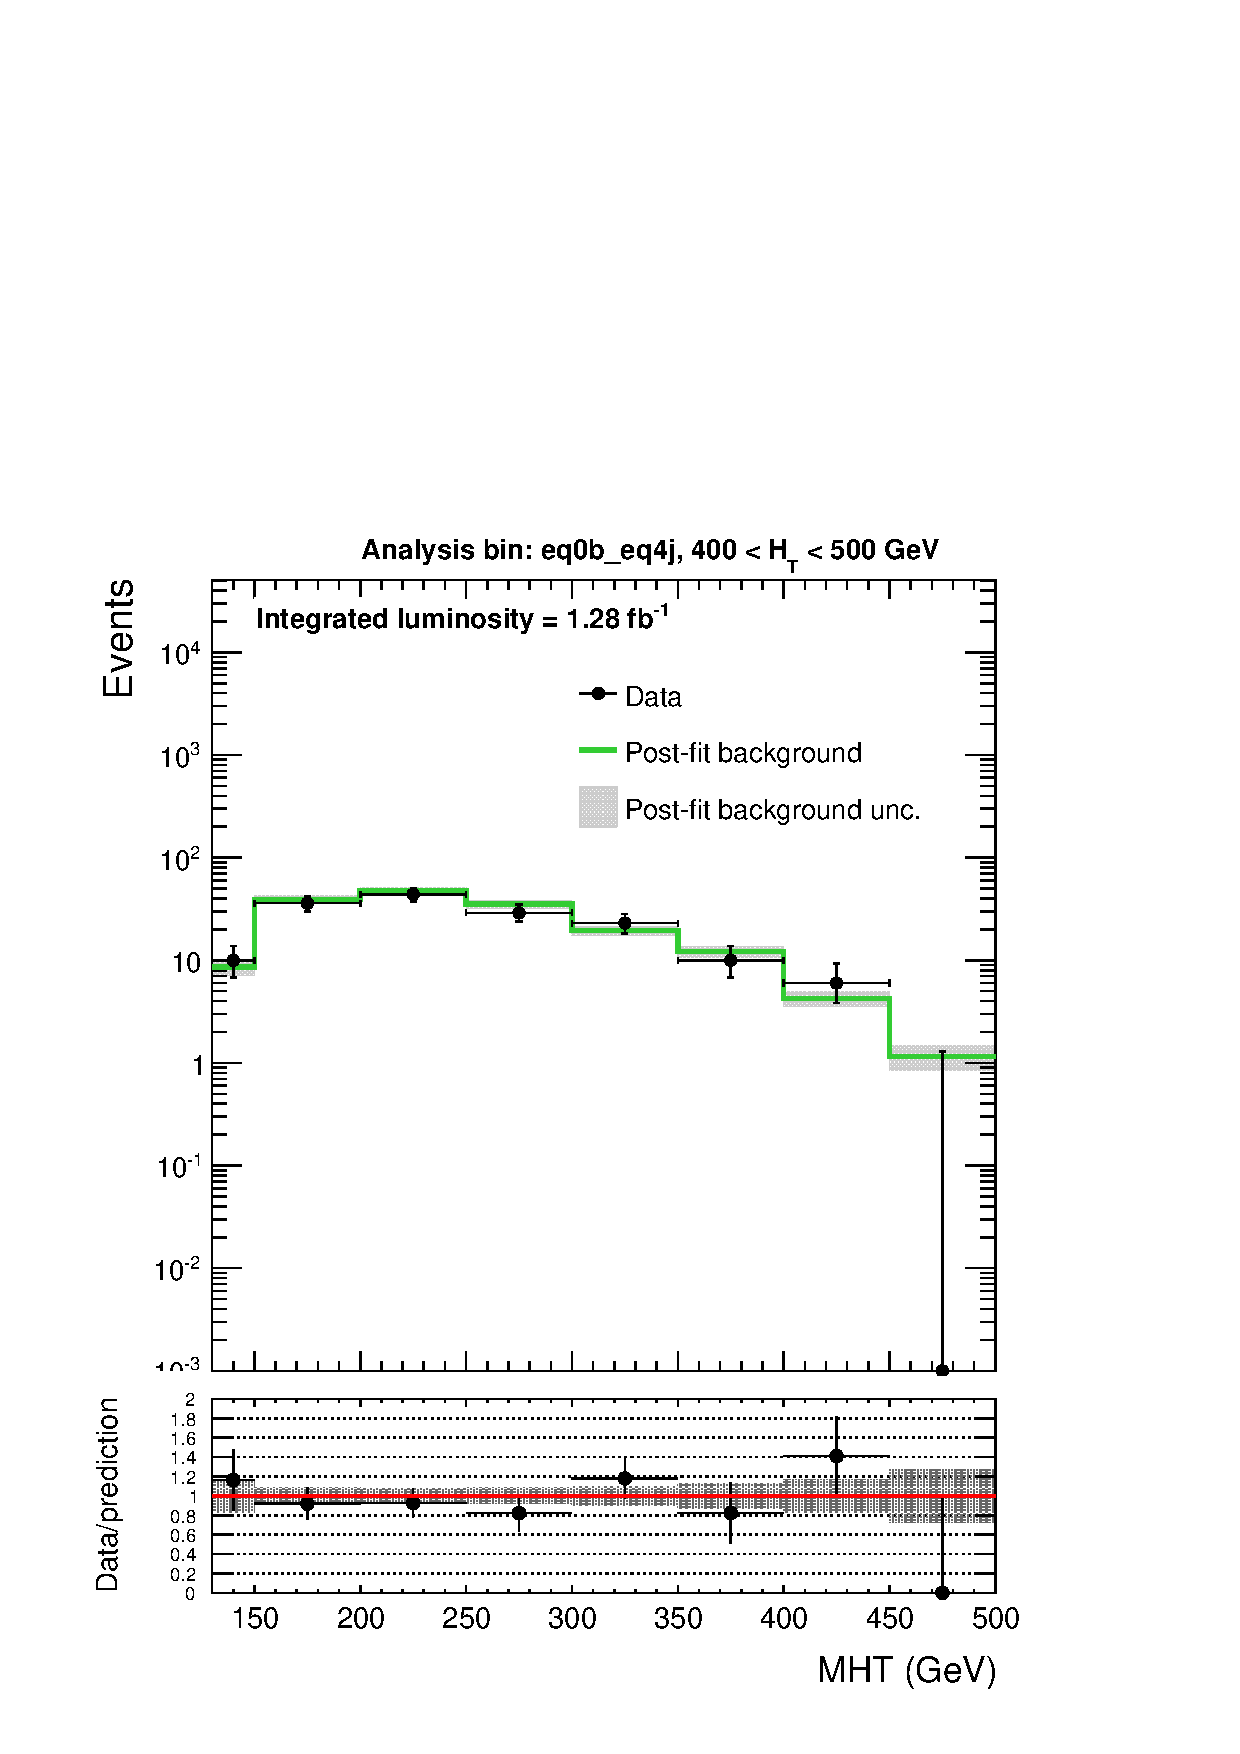
\includegraphics[width=0.25\textwidth]{figures/postFitResults/postFitShape_eq0b_eq4j_400_500.pdf} }\\
    \subfigure[$\nj^{\mathrm{sym}}=4$, $\nb=0$, $500 < \scalht < 600 \; \mathrm{GeV}$]{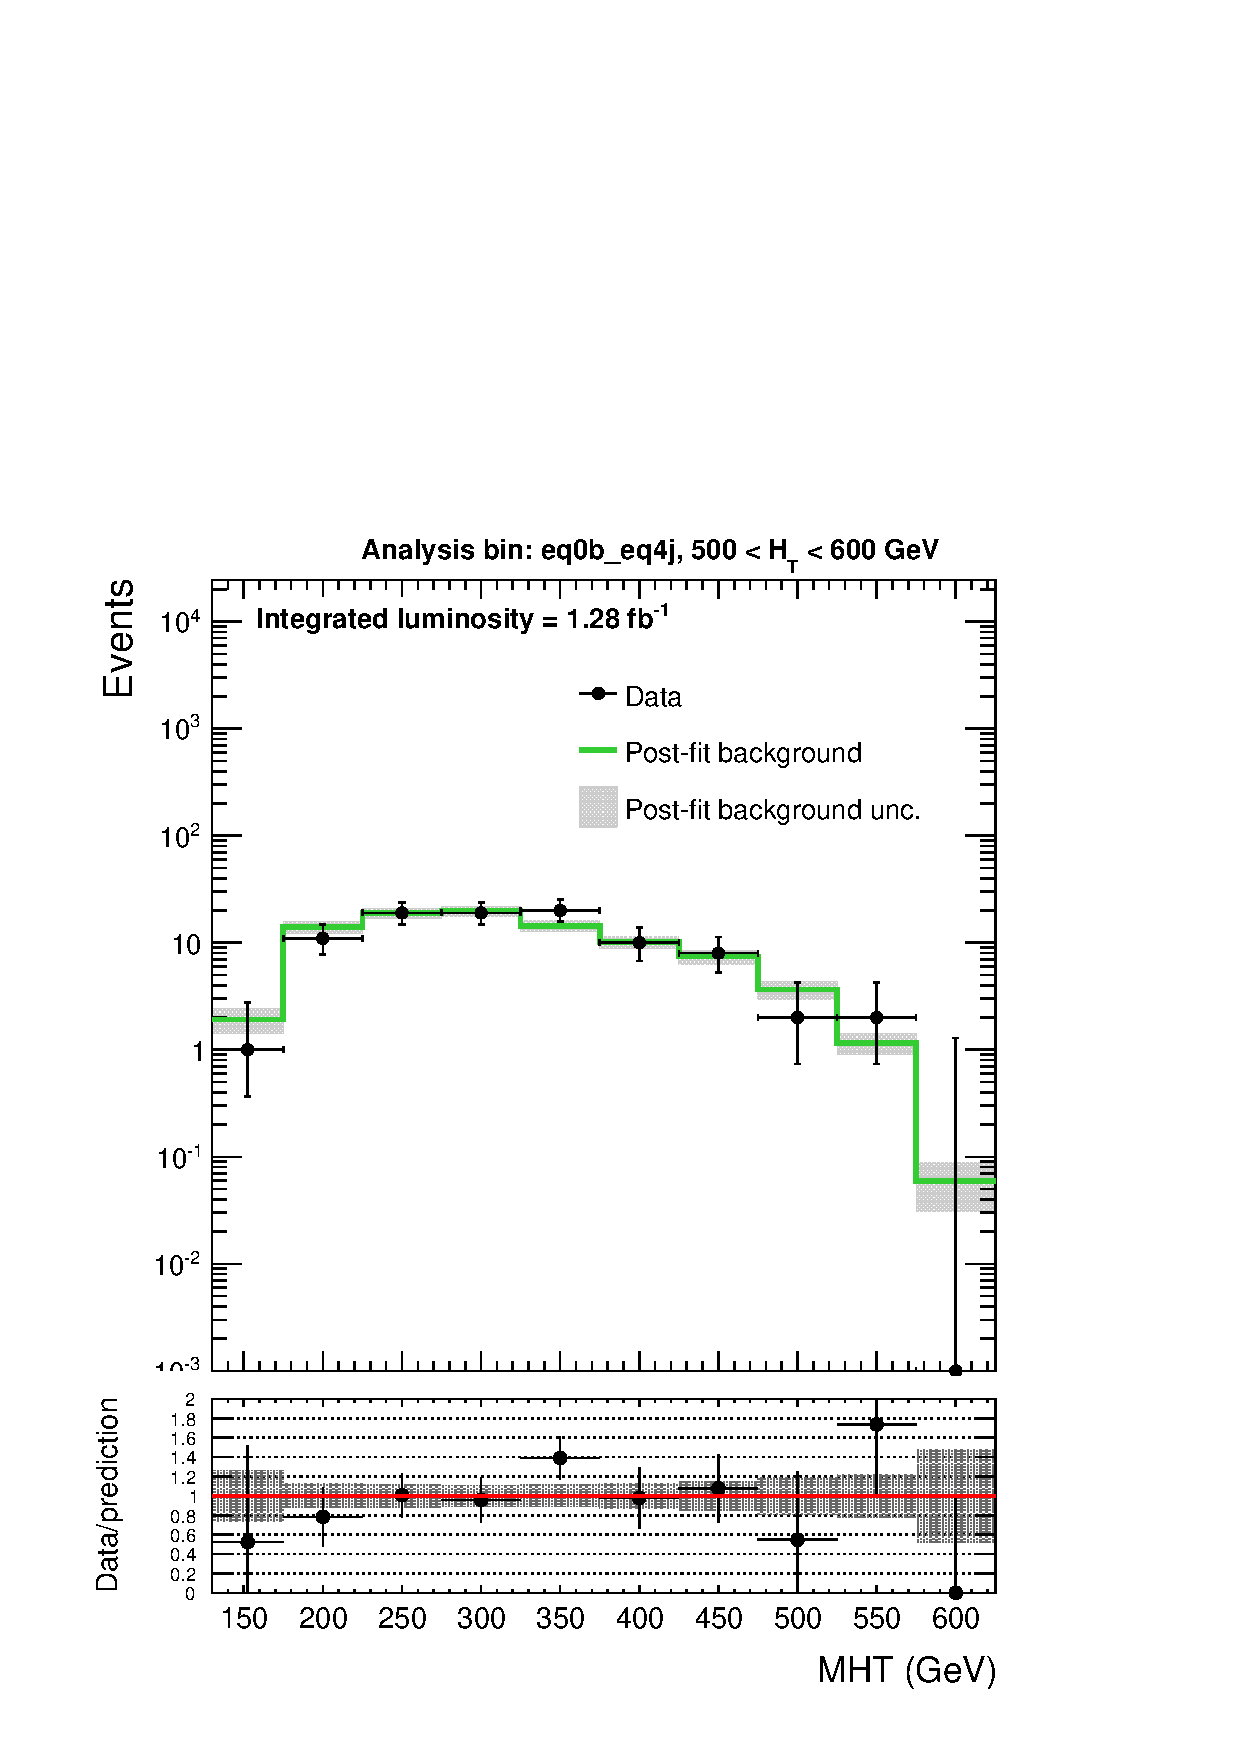
\includegraphics[width=0.25\textwidth]{figures/postFitResults/postFitShape_eq0b_eq4j_500_600.pdf} }\hspace{1cm}
    \subfigure[$\nj^{\mathrm{sym}}=4$, $\nb=0$, $600 < \scalht < 800 \; \mathrm{GeV}$]{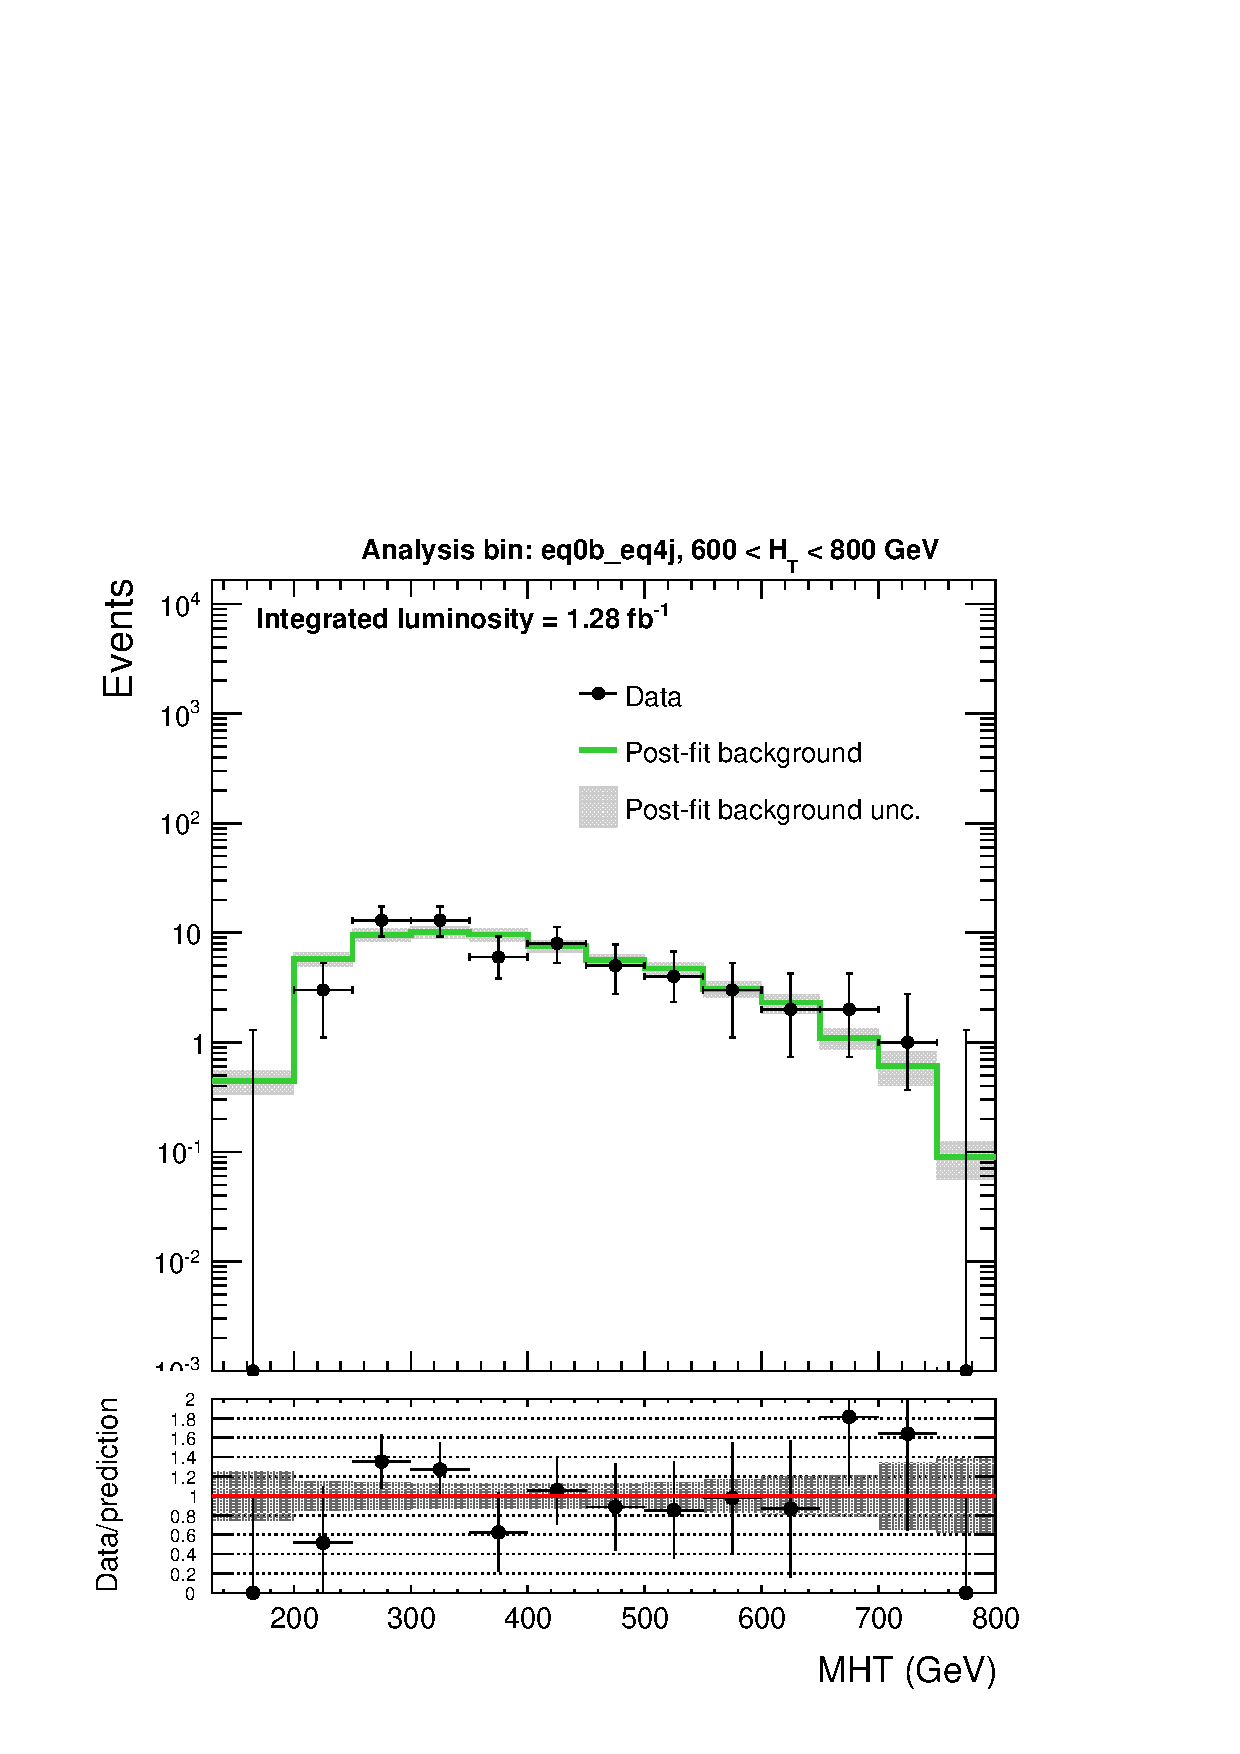
\includegraphics[width=0.25\textwidth]{figures/postFitResults/postFitShape_eq0b_eq4j_600_800.pdf} }\hspace{1cm}
    \subfigure[$\nj^{\mathrm{sym}}=4$, $\nb=0$, $\scalht > 800 \; \mathrm{GeV}$]{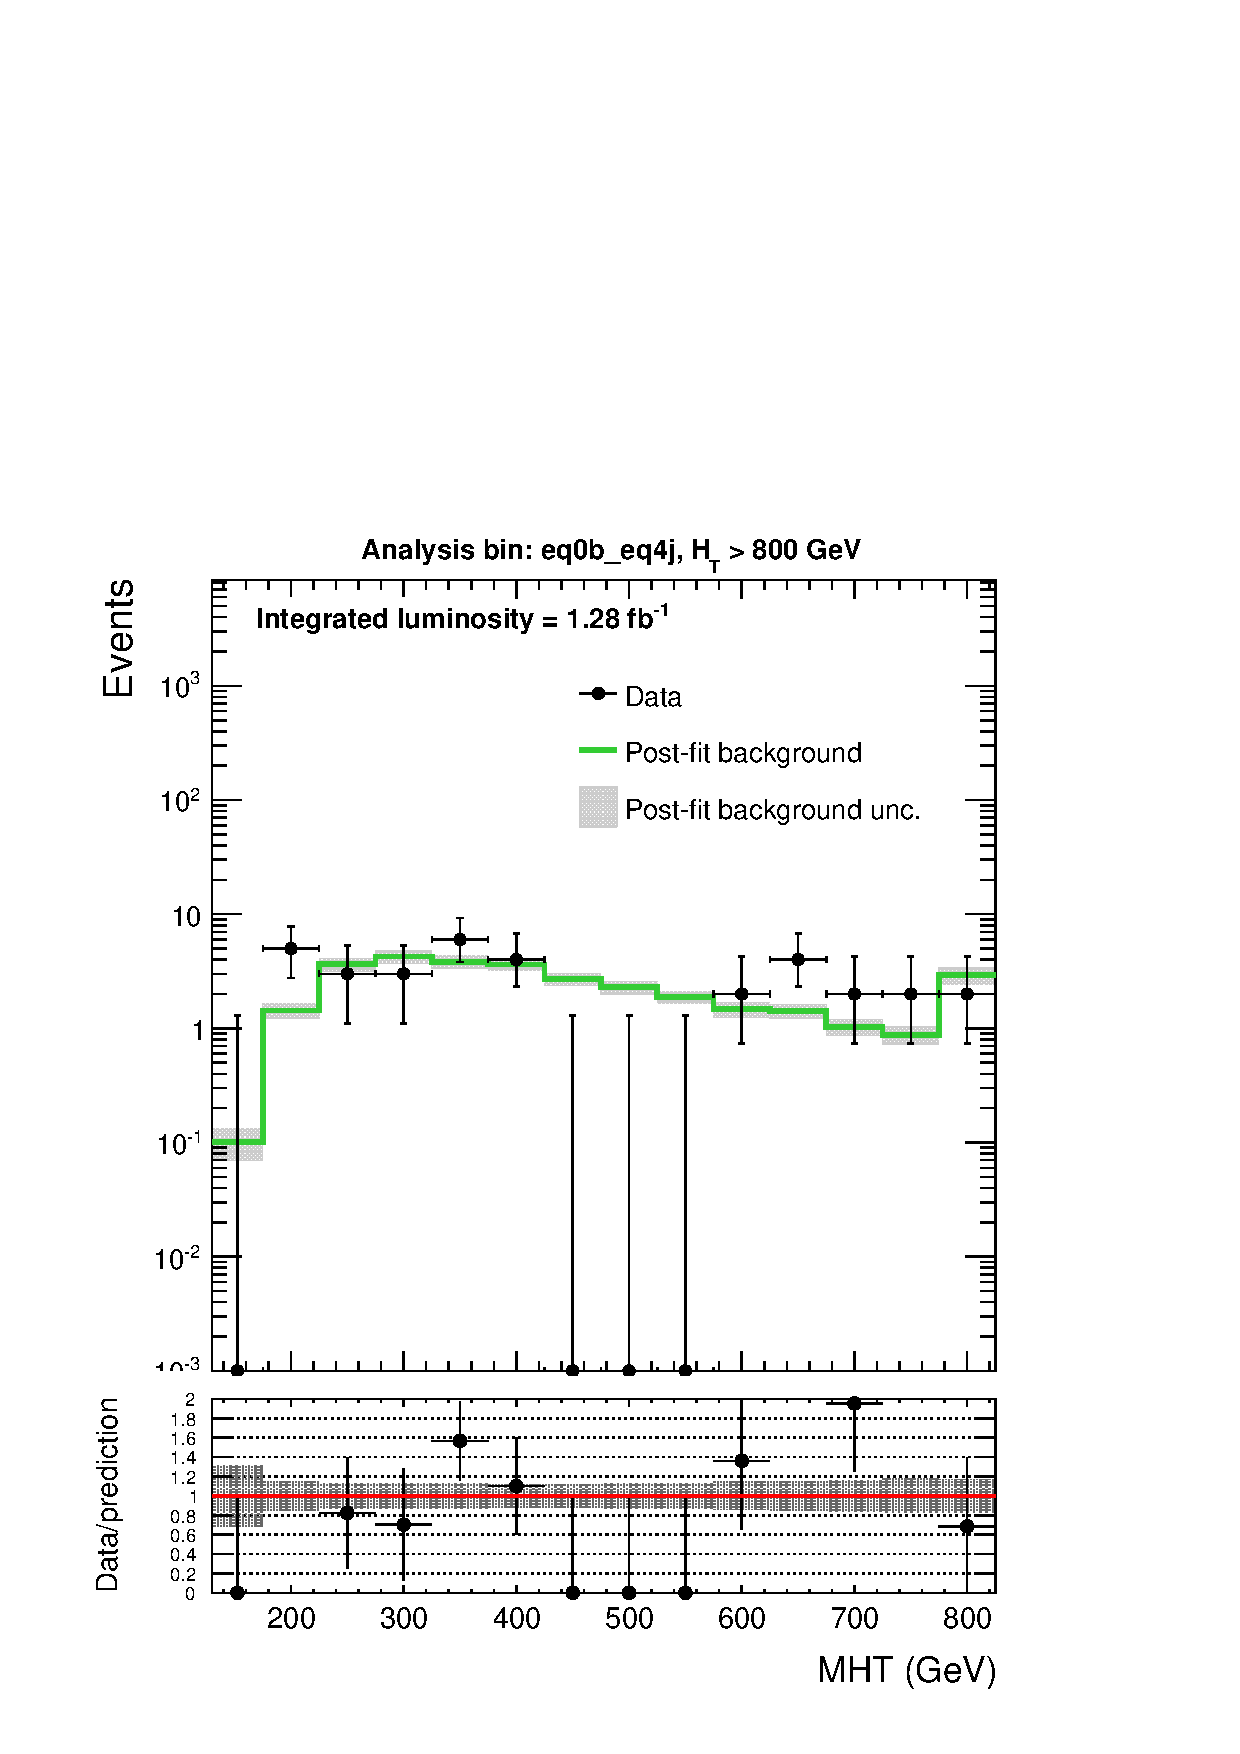
\includegraphics[width=0.25\textwidth]{figures/postFitResults/postFitShape_eq0b_eq4j_800_Inf.pdf} }\\
  \end{center}
\end{figure}



\newpage
\begin{figure}[h!]
\caption{Post-fit \MHT templates for the bin $\nj^{\mathrm{asym}}=5$, $\nb=0$ \label{fig:postFitShapes_eq0b_ge5a}}.
\begin{center}

    \subfigure[$\nj^{\mathrm{asym}}=5$, $\nb=0$, $300 < \scalht < 350 \; \mathrm{GeV}$]{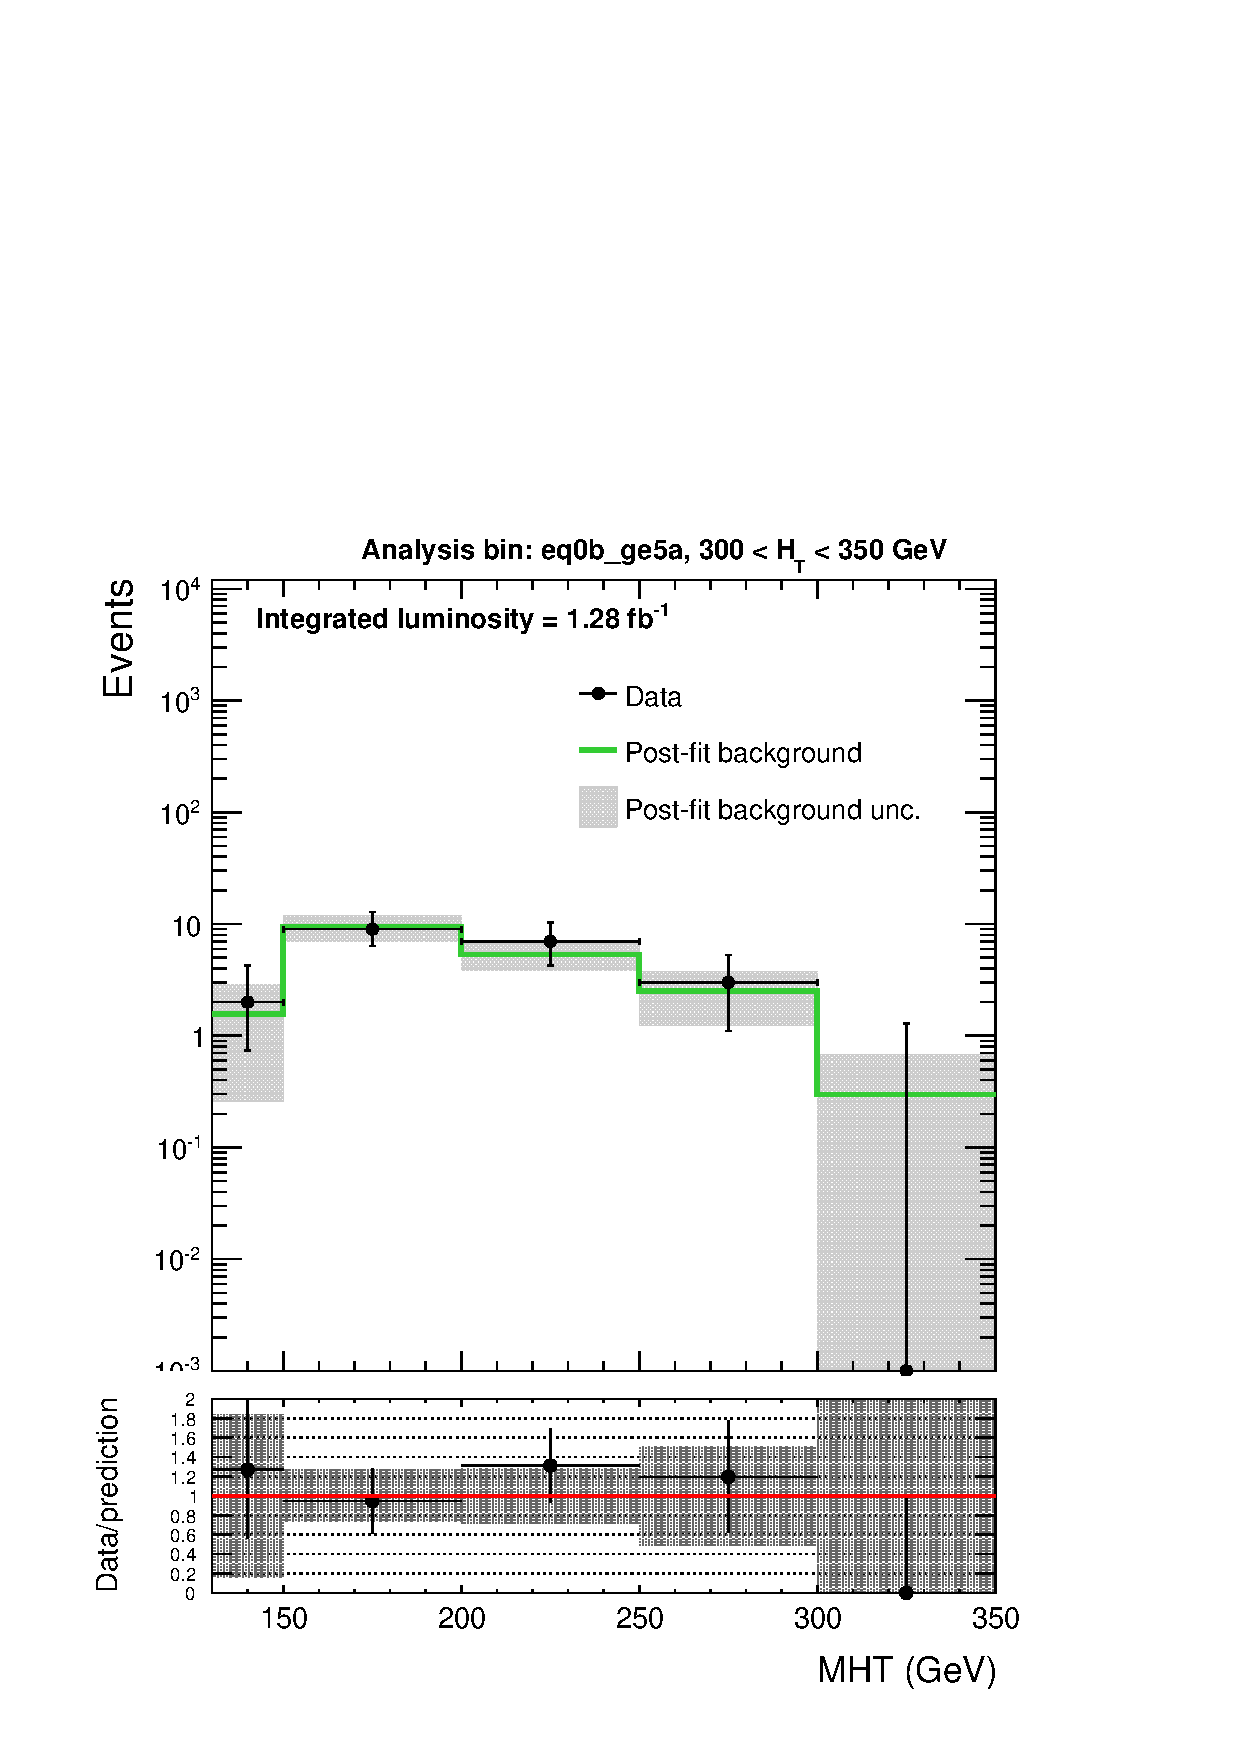
\includegraphics[width=0.25\textwidth]{figures/postFitResults/postFitShape_eq0b_ge5a_300_350.pdf} }\hspace{1cm}
    \subfigure[$\nj^{\mathrm{asym}}=5$, $\nb=0$, $350 < \scalht < 400 \; \mathrm{GeV}$]{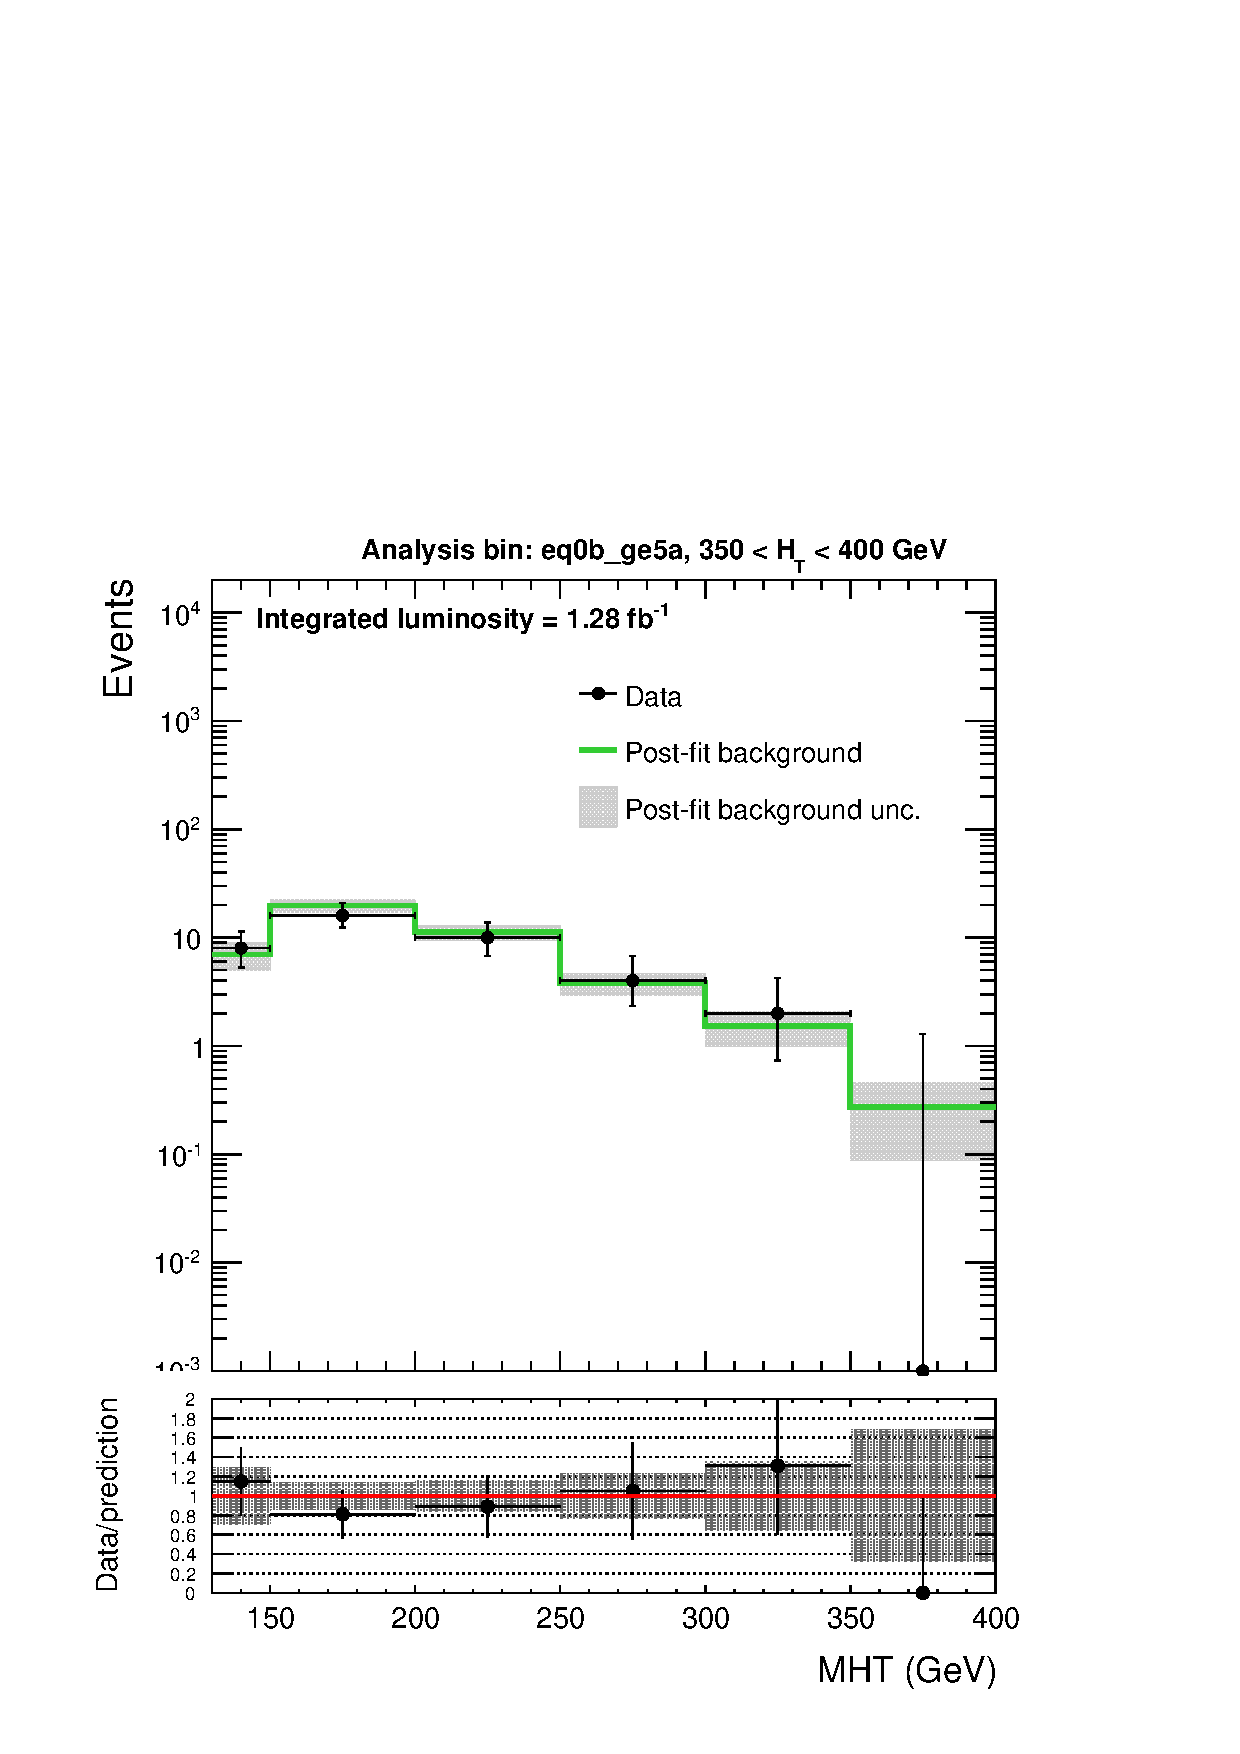
\includegraphics[width=0.25\textwidth]{figures/postFitResults/postFitShape_eq0b_ge5a_350_400.pdf} }\hspace{1cm}
    \subfigure[$\nj^{\mathrm{asym}}=5$, $\nb=0$, $400 < \scalht < 500 \; \mathrm{GeV}$]{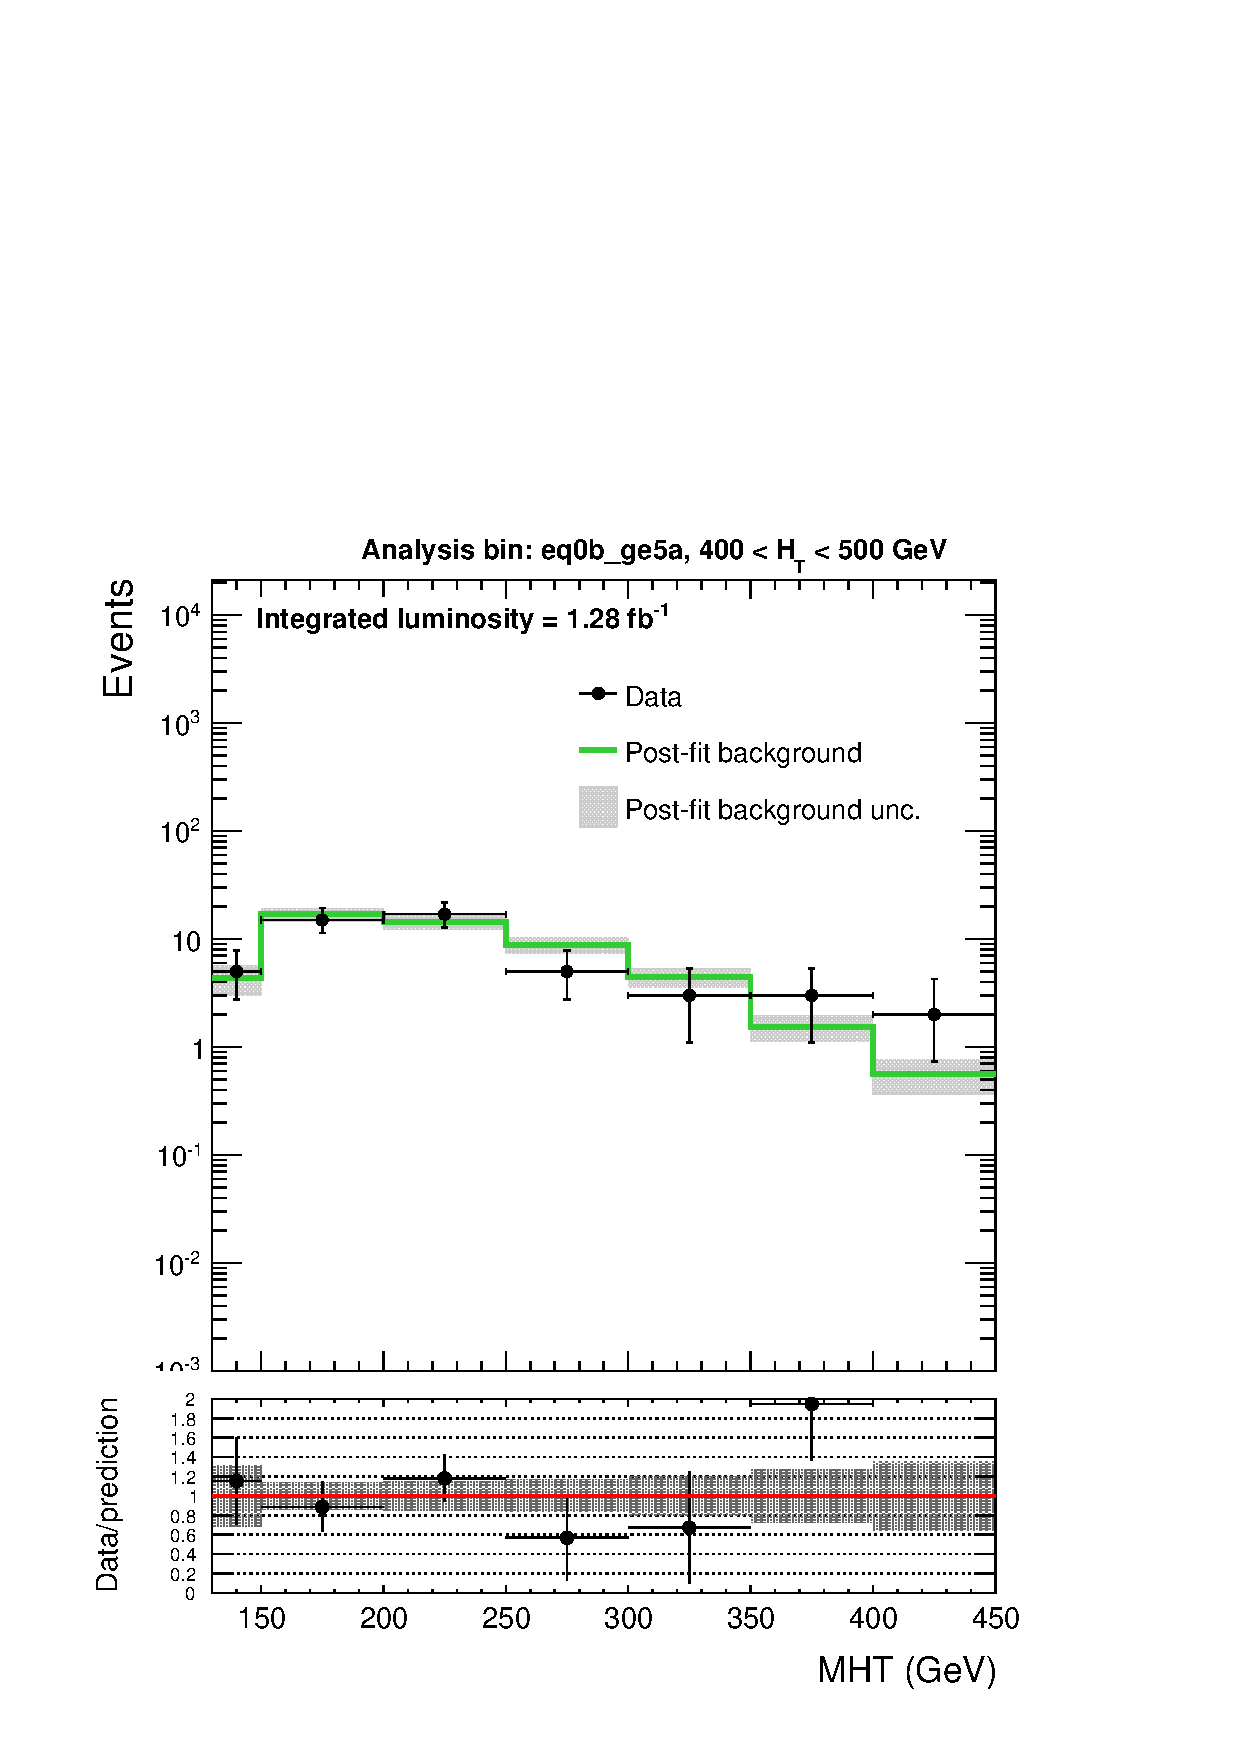
\includegraphics[width=0.25\textwidth]{figures/postFitResults/postFitShape_eq0b_ge5a_400_500.pdf} }\\
    \subfigure[$\nj^{\mathrm{asym}}=5$, $\nb=0$, $500 < \scalht < 600 \; \mathrm{GeV}$]{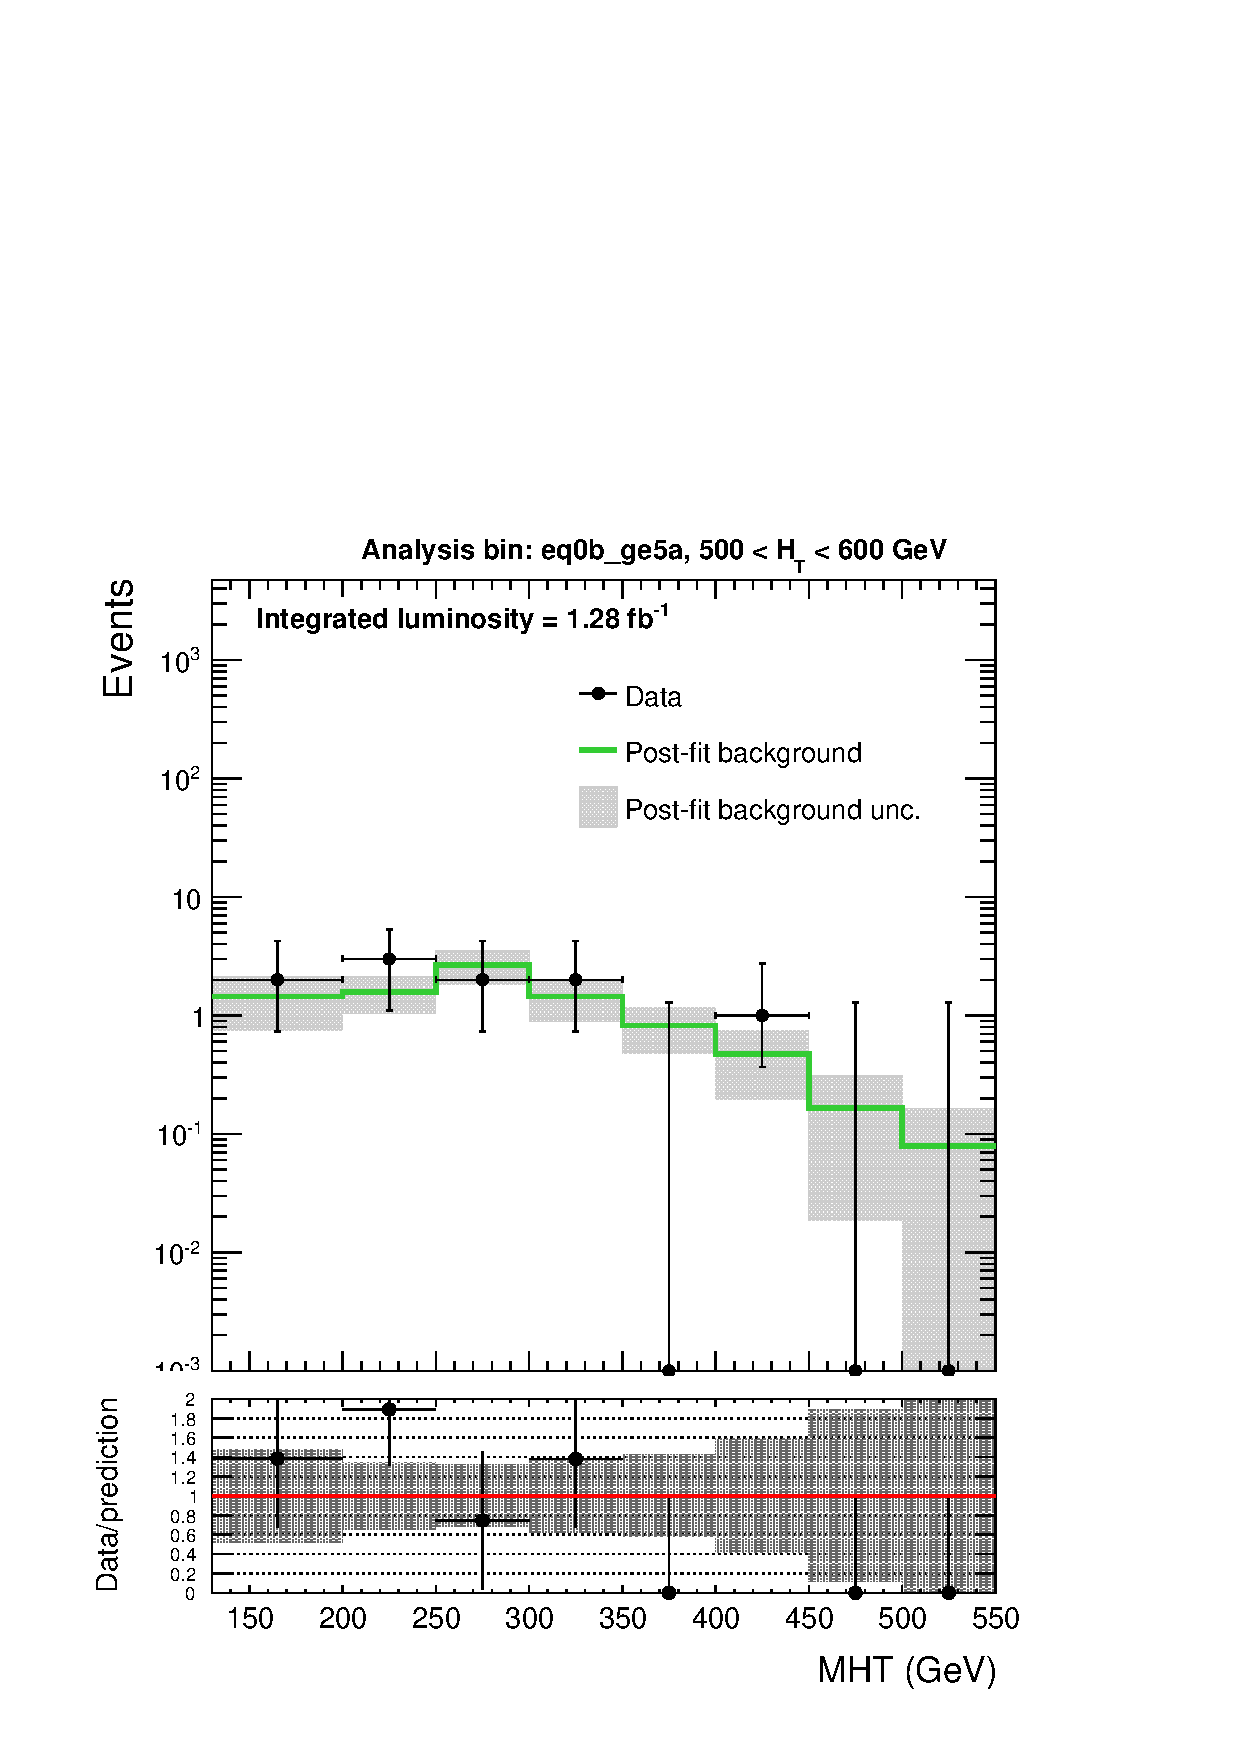
\includegraphics[width=0.25\textwidth]{figures/postFitResults/postFitShape_eq0b_ge5a_500_600.pdf} }\hspace{1cm}
  \end{center}
\end{figure}



\newpage
\begin{figure}[h!]
\caption{Post-fit \MHT templates for the bin $\nj^{\mathrm{sym}}=5$, $\nb=0$ \label{fig:postFitShapes_eq0b_ge5j}}.
\begin{center}

    \subfigure[$\nj^{\mathrm{sym}}=5$, $\nb=0$, $350 < \scalht < 400 \; \mathrm{GeV}$]{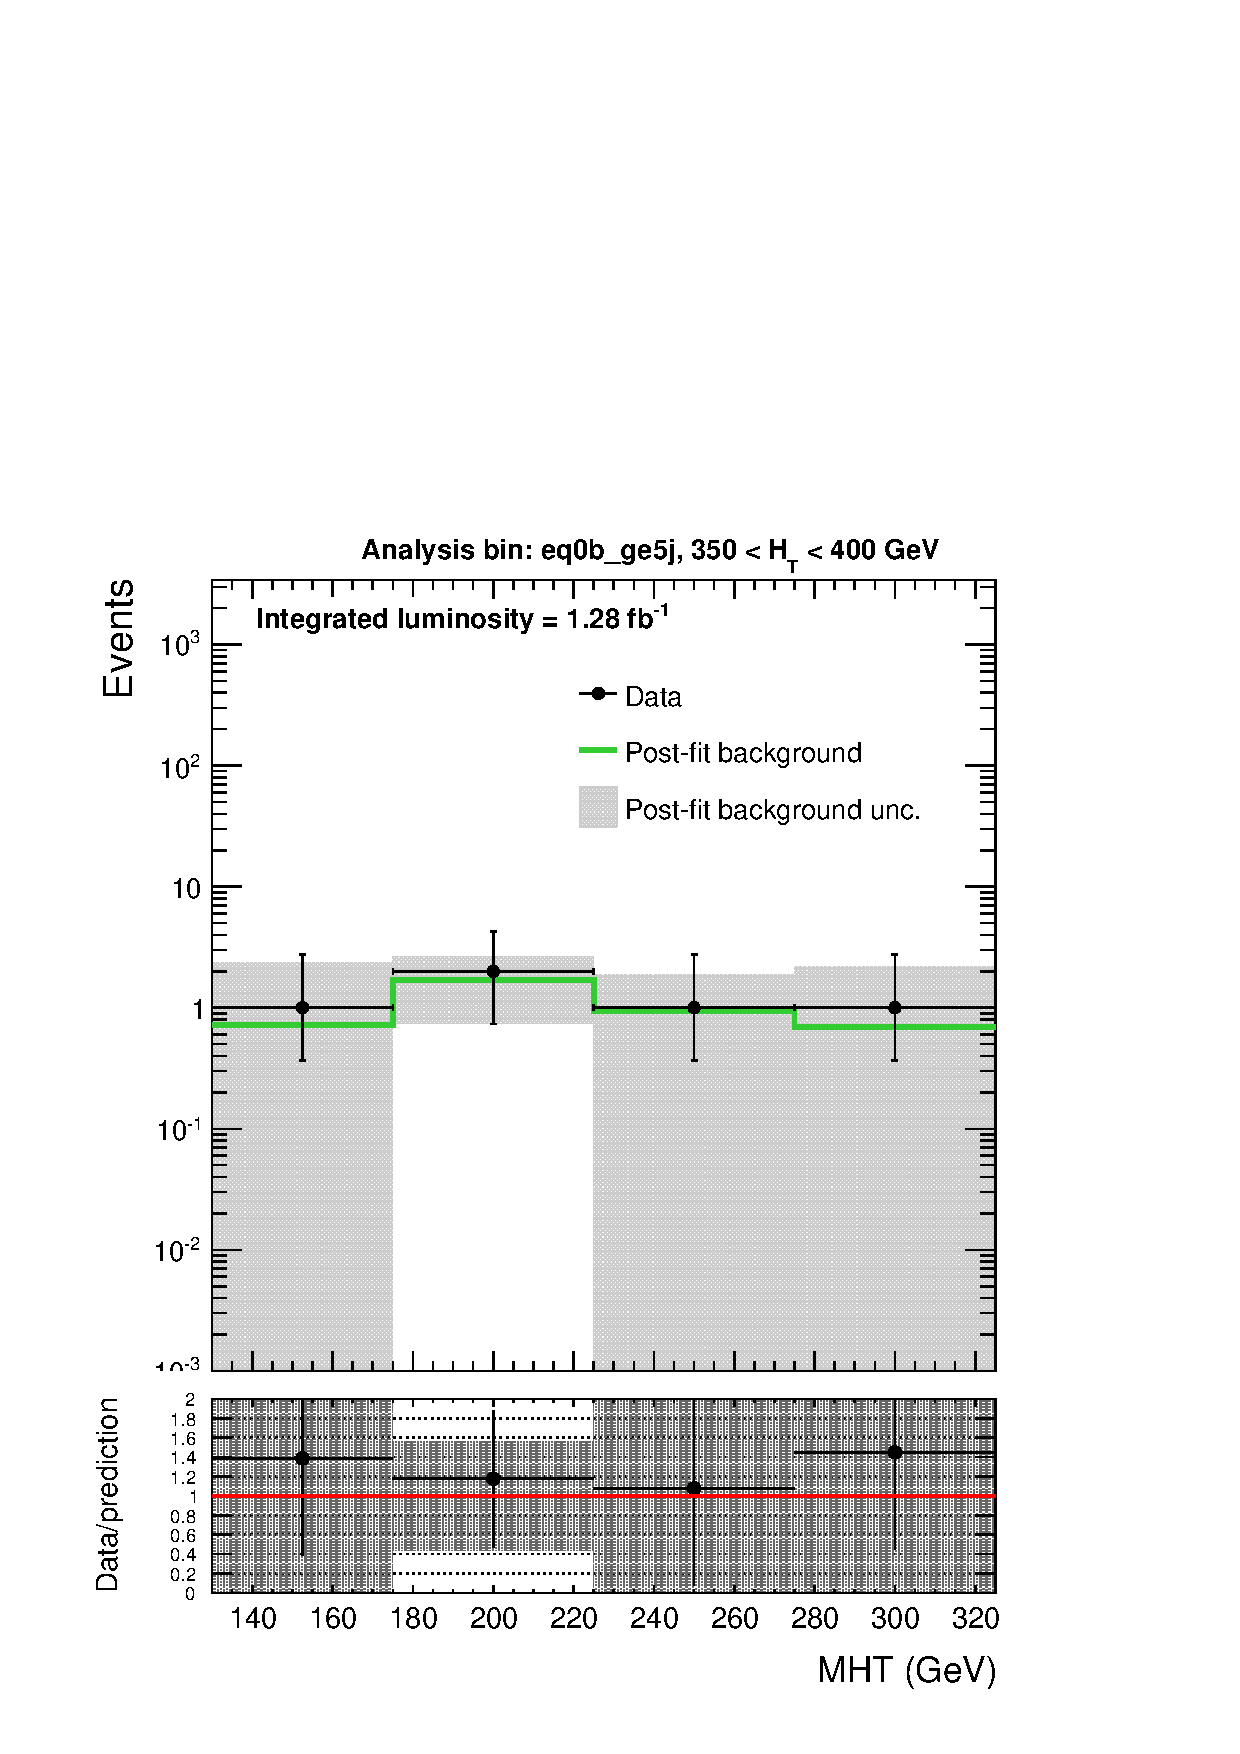
\includegraphics[width=0.25\textwidth]{figures/postFitResults/postFitShape_eq0b_ge5j_350_400.pdf} }\hspace{1cm}
    \subfigure[$\nj^{\mathrm{sym}}=5$, $\nb=0$, $400 < \scalht < 500 \; \mathrm{GeV}$]{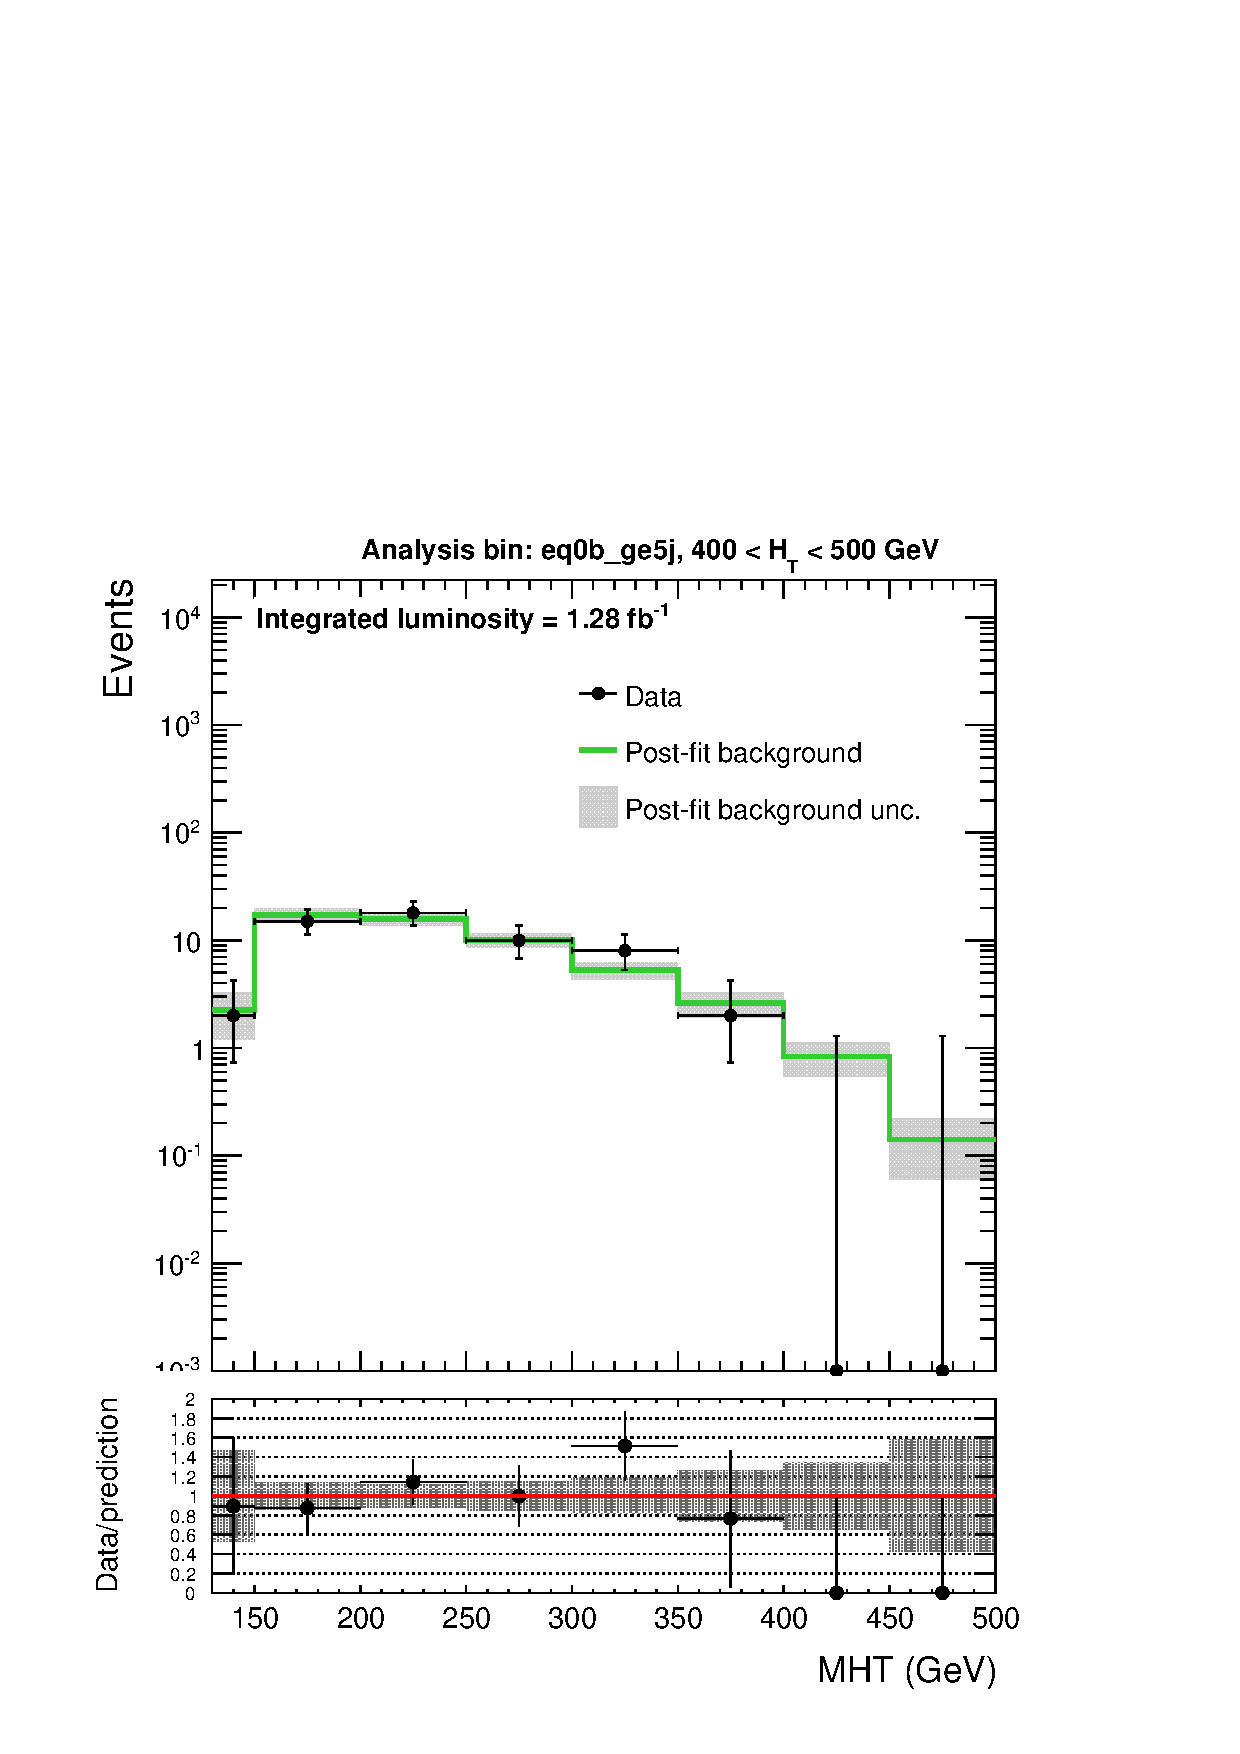
\includegraphics[width=0.25\textwidth]{figures/postFitResults/postFitShape_eq0b_ge5j_400_500.pdf} }\hspace{1cm}
    \subfigure[$\nj^{\mathrm{sym}}=5$, $\nb=0$, $500 < \scalht < 600 \; \mathrm{GeV}$]{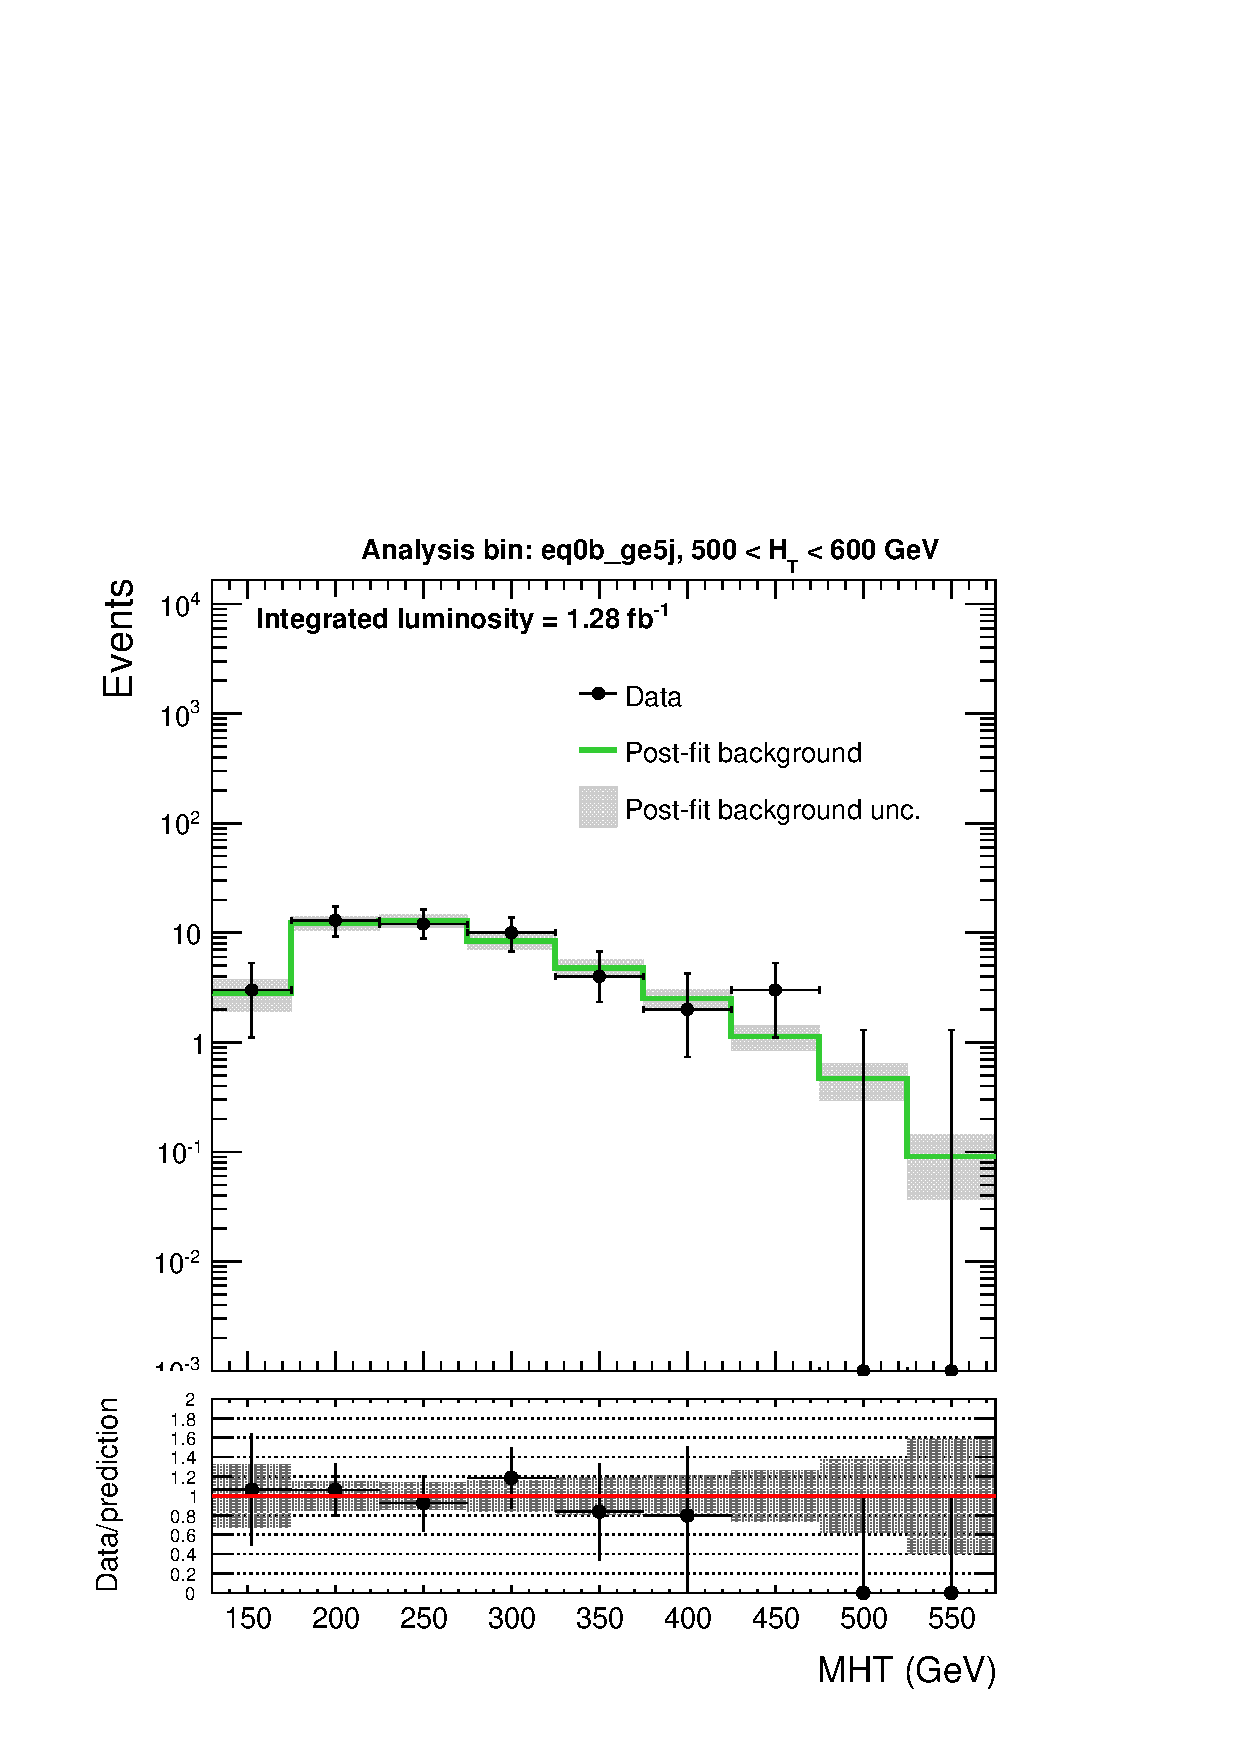
\includegraphics[width=0.25\textwidth]{figures/postFitResults/postFitShape_eq0b_ge5j_500_600.pdf} }\\
    \subfigure[$\nj^{\mathrm{sym}}=5$, $\nb=0$, $600 < \scalht < 800 \; \mathrm{GeV}$]{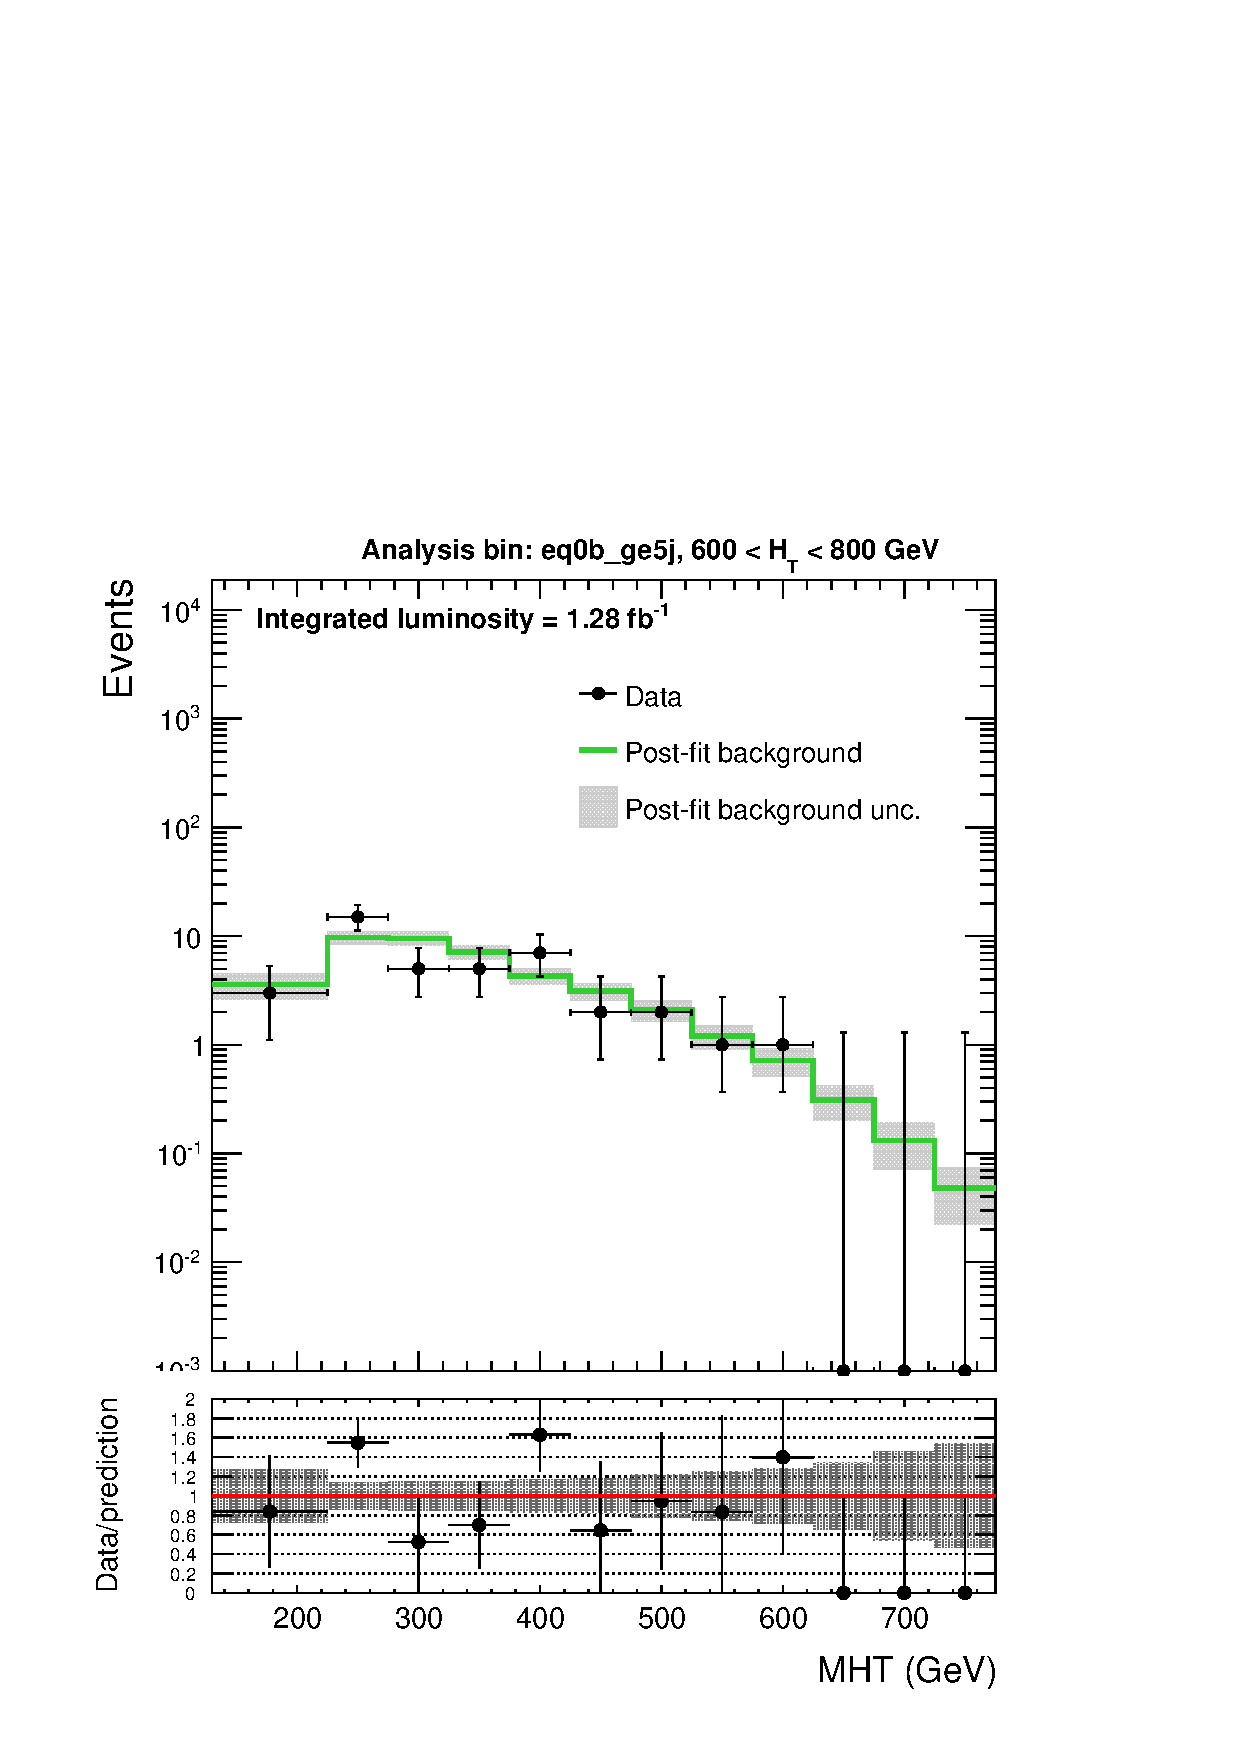
\includegraphics[width=0.25\textwidth]{figures/postFitResults/postFitShape_eq0b_ge5j_600_800.pdf} }\hspace{1cm}
    \subfigure[$\nj^{\mathrm{sym}}=5$, $\nb=0$, $\scalht > 800 \; \mathrm{GeV}$]{\includegraphics[width=0.25\textwidth]{figures/postFitResults/postFitShape_eq0b_ge5j_800_Inf.pdf} }\hspace{1cm}
  \end{center}
\end{figure}



\newpage
\begin{figure}[h!]
\caption{Post-fit \MHT templates for the bin $\nj^{\mathrm{asym}}=2$, $\nb=1$ \label{fig:postFitShapes_eq1b_eq2a}}.
\begin{center}

    \subfigure[$\nj^{\mathrm{asym}}=2$, $\nb=1$, $200 < \scalht < 250 \; \mathrm{GeV}$]{\includegraphics[width=0.25\textwidth]{figures/postFitResults/postFitShape_eq1b_eq2a_200_250.pdf} }\hspace{1cm}
    \subfigure[$\nj^{\mathrm{asym}}=2$, $\nb=1$, $250 < \scalht < 300 \; \mathrm{GeV}$]{\includegraphics[width=0.25\textwidth]{figures/postFitResults/postFitShape_eq1b_eq2a_250_300.pdf} }\hspace{1cm}
    \subfigure[$\nj^{\mathrm{asym}}=2$, $\nb=1$, $300 < \scalht < 350 \; \mathrm{GeV}$]{\includegraphics[width=0.25\textwidth]{figures/postFitResults/postFitShape_eq1b_eq2a_300_350.pdf} }\\
    \subfigure[$\nj^{\mathrm{asym}}=2$, $\nb=1$, $350 < \scalht < 400 \; \mathrm{GeV}$]{\includegraphics[width=0.25\textwidth]{figures/postFitResults/postFitShape_eq1b_eq2a_350_400.pdf} }\hspace{1cm}
    \subfigure[$\nj^{\mathrm{asym}}=2$, $\nb=1$, $400 < \scalht < 500 \; \mathrm{GeV}$]{\includegraphics[width=0.25\textwidth]{figures/postFitResults/postFitShape_eq1b_eq2a_400_500.pdf} }\hspace{1cm}
    \subfigure[$\nj^{\mathrm{asym}}=2$, $\nb=1$, $500 < \scalht < 600 \; \mathrm{GeV}$]{\includegraphics[width=0.25\textwidth]{figures/postFitResults/postFitShape_eq1b_eq2a_500_600.pdf} }\\
  \end{center}
\end{figure}



\newpage
\begin{figure}[h!]
\caption{Post-fit \MHT templates for the bin $\nj^{\mathrm{sym}}=2$, $\nb=1$ \label{fig:postFitShapes_eq1b_eq2j}}.
\begin{center}

    \subfigure[$\nj^{\mathrm{sym}}=2$, $\nb=1$, $200 < \scalht < 250 \; \mathrm{GeV}$]{\includegraphics[width=0.25\textwidth]{figures/postFitResults/postFitShape_eq1b_eq2j_200_250.pdf} }\hspace{1cm}
    \subfigure[$\nj^{\mathrm{sym}}=2$, $\nb=1$, $250 < \scalht < 300 \; \mathrm{GeV}$]{\includegraphics[width=0.25\textwidth]{figures/postFitResults/postFitShape_eq1b_eq2j_250_300.pdf} }\hspace{1cm}
    \subfigure[$\nj^{\mathrm{sym}}=2$, $\nb=1$, $300 < \scalht < 350 \; \mathrm{GeV}$]{\includegraphics[width=0.25\textwidth]{figures/postFitResults/postFitShape_eq1b_eq2j_300_350.pdf} }\\
    \subfigure[$\nj^{\mathrm{sym}}=2$, $\nb=1$, $350 < \scalht < 400 \; \mathrm{GeV}$]{\includegraphics[width=0.25\textwidth]{figures/postFitResults/postFitShape_eq1b_eq2j_350_400.pdf} }\hspace{1cm}
    \subfigure[$\nj^{\mathrm{sym}}=2$, $\nb=1$, $400 < \scalht < 500 \; \mathrm{GeV}$]{\includegraphics[width=0.25\textwidth]{figures/postFitResults/postFitShape_eq1b_eq2j_400_500.pdf} }\hspace{1cm}
    \subfigure[$\nj^{\mathrm{sym}}=2$, $\nb=1$, $500 < \scalht < 600 \; \mathrm{GeV}$]{\includegraphics[width=0.25\textwidth]{figures/postFitResults/postFitShape_eq1b_eq2j_500_600.pdf} }\\
    \subfigure[$\nj^{\mathrm{sym}}=2$, $\nb=1$, $600 < \scalht < 800 \; \mathrm{GeV}$]{\includegraphics[width=0.25\textwidth]{figures/postFitResults/postFitShape_eq1b_eq2j_600_800.pdf} }\hspace{1cm}
    \subfigure[$\nj^{\mathrm{sym}}=2$, $\nb=1$, $\scalht > 800 \; \mathrm{GeV}$]{\includegraphics[width=0.25\textwidth]{figures/postFitResults/postFitShape_eq1b_eq2j_800_Inf.pdf} }\hspace{1cm}
  \end{center}
\end{figure}



\newpage
\begin{figure}[h!]
\caption{Post-fit \MHT templates for the bin $\nj^{\mathrm{asym}}=3$, $\nb=1$ \label{fig:postFitShapes_eq1b_eq3a}}.
\begin{center}

    \subfigure[$\nj^{\mathrm{asym}}=3$, $\nb=1$, $200 < \scalht < 250 \; \mathrm{GeV}$]{\includegraphics[width=0.25\textwidth]{figures/postFitResults/postFitShape_eq1b_eq3a_200_250.pdf} }\hspace{1cm}
    \subfigure[$\nj^{\mathrm{asym}}=3$, $\nb=1$, $250 < \scalht < 300 \; \mathrm{GeV}$]{\includegraphics[width=0.25\textwidth]{figures/postFitResults/postFitShape_eq1b_eq3a_250_300.pdf} }\hspace{1cm}
    \subfigure[$\nj^{\mathrm{asym}}=3$, $\nb=1$, $300 < \scalht < 350 \; \mathrm{GeV}$]{\includegraphics[width=0.25\textwidth]{figures/postFitResults/postFitShape_eq1b_eq3a_300_350.pdf} }\\
    \subfigure[$\nj^{\mathrm{asym}}=3$, $\nb=1$, $350 < \scalht < 400 \; \mathrm{GeV}$]{\includegraphics[width=0.25\textwidth]{figures/postFitResults/postFitShape_eq1b_eq3a_350_400.pdf} }\hspace{1cm}
    \subfigure[$\nj^{\mathrm{asym}}=3$, $\nb=1$, $400 < \scalht < 500 \; \mathrm{GeV}$]{\includegraphics[width=0.25\textwidth]{figures/postFitResults/postFitShape_eq1b_eq3a_400_500.pdf} }\hspace{1cm}
    \subfigure[$\nj^{\mathrm{asym}}=3$, $\nb=1$, $500 < \scalht < 600 \; \mathrm{GeV}$]{\includegraphics[width=0.25\textwidth]{figures/postFitResults/postFitShape_eq1b_eq3a_500_600.pdf} }\\
    \subfigure[$\nj^{\mathrm{asym}}=3$, $\nb=1$, $\scalht > 600 \; \mathrm{GeV}$]{\includegraphics[width=0.25\textwidth]{figures/postFitResults/postFitShape_eq1b_eq3a_600_Inf.pdf} }\hspace{1cm}
  \end{center}
\end{figure}



\newpage
\begin{figure}[h!]
\caption{Post-fit \MHT templates for the bin $\nj^{\mathrm{sym}}=3$, $\nb=1$ \label{fig:postFitShapes_eq1b_eq3j}}.
\begin{center}

    \subfigure[$\nj^{\mathrm{sym}}=3$, $\nb=1$, $250 < \scalht < 300 \; \mathrm{GeV}$]{\includegraphics[width=0.25\textwidth]{figures/postFitResults/postFitShape_eq1b_eq3j_250_300.pdf} }\hspace{1cm}
    \subfigure[$\nj^{\mathrm{sym}}=3$, $\nb=1$, $300 < \scalht < 350 \; \mathrm{GeV}$]{\includegraphics[width=0.25\textwidth]{figures/postFitResults/postFitShape_eq1b_eq3j_300_350.pdf} }\hspace{1cm}
    \subfigure[$\nj^{\mathrm{sym}}=3$, $\nb=1$, $350 < \scalht < 400 \; \mathrm{GeV}$]{\includegraphics[width=0.25\textwidth]{figures/postFitResults/postFitShape_eq1b_eq3j_350_400.pdf} }\\
    \subfigure[$\nj^{\mathrm{sym}}=3$, $\nb=1$, $400 < \scalht < 500 \; \mathrm{GeV}$]{\includegraphics[width=0.25\textwidth]{figures/postFitResults/postFitShape_eq1b_eq3j_400_500.pdf} }\hspace{1cm}
    \subfigure[$\nj^{\mathrm{sym}}=3$, $\nb=1$, $500 < \scalht < 600 \; \mathrm{GeV}$]{\includegraphics[width=0.25\textwidth]{figures/postFitResults/postFitShape_eq1b_eq3j_500_600.pdf} }\hspace{1cm}
    \subfigure[$\nj^{\mathrm{sym}}=3$, $\nb=1$, $600 < \scalht < 800 \; \mathrm{GeV}$]{\includegraphics[width=0.25\textwidth]{figures/postFitResults/postFitShape_eq1b_eq3j_600_800.pdf} }\\
    \subfigure[$\nj^{\mathrm{sym}}=3$, $\nb=1$, $\scalht > 800 \; \mathrm{GeV}$]{\includegraphics[width=0.25\textwidth]{figures/postFitResults/postFitShape_eq1b_eq3j_800_Inf.pdf} }\hspace{1cm}
  \end{center}
\end{figure}



\newpage
\begin{figure}[h!]
\caption{Post-fit \MHT templates for the bin $\nj^{\mathrm{asym}}=4$, $\nb=1$ \label{fig:postFitShapes_eq1b_eq4a}}.
\begin{center}

    \subfigure[$\nj^{\mathrm{asym}}=4$, $\nb=1$, $250 < \scalht < 300 \; \mathrm{GeV}$]{\includegraphics[width=0.25\textwidth]{figures/postFitResults/postFitShape_eq1b_eq4a_250_300.pdf} }\hspace{1cm}
    \subfigure[$\nj^{\mathrm{asym}}=4$, $\nb=1$, $300 < \scalht < 350 \; \mathrm{GeV}$]{\includegraphics[width=0.25\textwidth]{figures/postFitResults/postFitShape_eq1b_eq4a_300_350.pdf} }\hspace{1cm}
    \subfigure[$\nj^{\mathrm{asym}}=4$, $\nb=1$, $350 < \scalht < 400 \; \mathrm{GeV}$]{\includegraphics[width=0.25\textwidth]{figures/postFitResults/postFitShape_eq1b_eq4a_350_400.pdf} }\\
    \subfigure[$\nj^{\mathrm{asym}}=4$, $\nb=1$, $400 < \scalht < 500 \; \mathrm{GeV}$]{\includegraphics[width=0.25\textwidth]{figures/postFitResults/postFitShape_eq1b_eq4a_400_500.pdf} }\hspace{1cm}
    \subfigure[$\nj^{\mathrm{asym}}=4$, $\nb=1$, $500 < \scalht < 600 \; \mathrm{GeV}$]{\includegraphics[width=0.25\textwidth]{figures/postFitResults/postFitShape_eq1b_eq4a_500_600.pdf} }\hspace{1cm}
    \subfigure[$\nj^{\mathrm{asym}}=4$, $\nb=1$, $\scalht > 600 \; \mathrm{GeV}$]{\includegraphics[width=0.25\textwidth]{figures/postFitResults/postFitShape_eq1b_eq4a_600_Inf.pdf} }\\
  \end{center}
\end{figure}



\newpage
\begin{figure}[h!]
\caption{Post-fit \MHT templates for the bin $\nj^{\mathrm{sym}}=4$, $\nb=1$ \label{fig:postFitShapes_eq1b_eq4j}}.
\begin{center}

    \subfigure[$\nj^{\mathrm{sym}}=4$, $\nb=1$, $300 < \scalht < 350 \; \mathrm{GeV}$]{\includegraphics[width=0.25\textwidth]{figures/postFitResults/postFitShape_eq1b_eq4j_300_350.pdf} }\hspace{1cm}
    \subfigure[$\nj^{\mathrm{sym}}=4$, $\nb=1$, $350 < \scalht < 400 \; \mathrm{GeV}$]{\includegraphics[width=0.25\textwidth]{figures/postFitResults/postFitShape_eq1b_eq4j_350_400.pdf} }\hspace{1cm}
    \subfigure[$\nj^{\mathrm{sym}}=4$, $\nb=1$, $400 < \scalht < 500 \; \mathrm{GeV}$]{\includegraphics[width=0.25\textwidth]{figures/postFitResults/postFitShape_eq1b_eq4j_400_500.pdf} }\\
    \subfigure[$\nj^{\mathrm{sym}}=4$, $\nb=1$, $500 < \scalht < 600 \; \mathrm{GeV}$]{\includegraphics[width=0.25\textwidth]{figures/postFitResults/postFitShape_eq1b_eq4j_500_600.pdf} }\hspace{1cm}
    \subfigure[$\nj^{\mathrm{sym}}=4$, $\nb=1$, $600 < \scalht < 800 \; \mathrm{GeV}$]{\includegraphics[width=0.25\textwidth]{figures/postFitResults/postFitShape_eq1b_eq4j_600_800.pdf} }\hspace{1cm}
    \subfigure[$\nj^{\mathrm{sym}}=4$, $\nb=1$, $\scalht > 800 \; \mathrm{GeV}$]{\includegraphics[width=0.25\textwidth]{figures/postFitResults/postFitShape_eq1b_eq4j_800_Inf.pdf} }\\
  \end{center}
\end{figure}



\newpage
\begin{figure}[h!]
\caption{Post-fit \MHT templates for the bin $\nj^{\mathrm{asym}}=5$, $\nb=1$ \label{fig:postFitShapes_eq1b_ge5a}}.
\begin{center}

    \subfigure[$\nj^{\mathrm{asym}}=5$, $\nb=1$, $300 < \scalht < 350 \; \mathrm{GeV}$]{\includegraphics[width=0.25\textwidth]{figures/postFitResults/postFitShape_eq1b_ge5a_300_350.pdf} }\hspace{1cm}
    \subfigure[$\nj^{\mathrm{asym}}=5$, $\nb=1$, $350 < \scalht < 400 \; \mathrm{GeV}$]{\includegraphics[width=0.25\textwidth]{figures/postFitResults/postFitShape_eq1b_ge5a_350_400.pdf} }\hspace{1cm}
    \subfigure[$\nj^{\mathrm{asym}}=5$, $\nb=1$, $400 < \scalht < 500 \; \mathrm{GeV}$]{\includegraphics[width=0.25\textwidth]{figures/postFitResults/postFitShape_eq1b_ge5a_400_500.pdf} }\\
    \subfigure[$\nj^{\mathrm{asym}}=5$, $\nb=1$, $500 < \scalht < 600 \; \mathrm{GeV}$]{\includegraphics[width=0.25\textwidth]{figures/postFitResults/postFitShape_eq1b_ge5a_500_600.pdf} }\hspace{1cm}
    \subfigure[$\nj^{\mathrm{asym}}=5$, $\nb=1$, $\scalht > 600 \; \mathrm{GeV}$]{\includegraphics[width=0.25\textwidth]{figures/postFitResults/postFitShape_eq1b_ge5a_600_Inf.pdf} }\hspace{1cm}
  \end{center}
\end{figure}



\newpage
\begin{figure}[h!]
\caption{Post-fit \MHT templates for the bin $\nj^{\mathrm{sym}}=5$, $\nb=1$ \label{fig:postFitShapes_eq1b_ge5j}}.
\begin{center}

    \subfigure[$\nj^{\mathrm{sym}}=5$, $\nb=1$, $400 < \scalht < 500 \; \mathrm{GeV}$]{\includegraphics[width=0.25\textwidth]{figures/postFitResults/postFitShape_eq1b_ge5j_400_500.pdf} }\hspace{1cm}
    \subfigure[$\nj^{\mathrm{sym}}=5$, $\nb=1$, $500 < \scalht < 600 \; \mathrm{GeV}$]{\includegraphics[width=0.25\textwidth]{figures/postFitResults/postFitShape_eq1b_ge5j_500_600.pdf} }\hspace{1cm}
    \subfigure[$\nj^{\mathrm{sym}}=5$, $\nb=1$, $600 < \scalht < 800 \; \mathrm{GeV}$]{\includegraphics[width=0.25\textwidth]{figures/postFitResults/postFitShape_eq1b_ge5j_600_800.pdf} }\\
    \subfigure[$\nj^{\mathrm{sym}}=5$, $\nb=1$, $\scalht > 800 \; \mathrm{GeV}$]{\includegraphics[width=0.25\textwidth]{figures/postFitResults/postFitShape_eq1b_ge5j_800_Inf.pdf} }\hspace{1cm}
  \end{center}
\end{figure}



\newpage
\begin{figure}[h!]
\caption{Post-fit \MHT templates for the bin $\nj^{\mathrm{asym}}=2$, $\nb=2$ \label{fig:postFitShapes_eq2b_eq2a}}.
\begin{center}

    \subfigure[$\nj^{\mathrm{asym}}=2$, $\nb=2$, $200 < \scalht < 250 \; \mathrm{GeV}$]{\includegraphics[width=0.25\textwidth]{figures/postFitResults/postFitShape_eq2b_eq2a_200_250.pdf} }\hspace{1cm}
    \subfigure[$\nj^{\mathrm{asym}}=2$, $\nb=2$, $250 < \scalht < 300 \; \mathrm{GeV}$]{\includegraphics[width=0.25\textwidth]{figures/postFitResults/postFitShape_eq2b_eq2a_250_300.pdf} }\hspace{1cm}
    \subfigure[$\nj^{\mathrm{asym}}=2$, $\nb=2$, $300 < \scalht < 350 \; \mathrm{GeV}$]{\includegraphics[width=0.25\textwidth]{figures/postFitResults/postFitShape_eq2b_eq2a_300_350.pdf} }\\
  \end{center}
\end{figure}



\newpage
\begin{figure}[h!]
\caption{Post-fit \MHT templates for the bin $\nj^{\mathrm{asym}}=3$, $\nb=2$ \label{fig:postFitShapes_eq2b_eq3a}}.
\begin{center}

    \subfigure[$\nj^{\mathrm{asym}}=3$, $\nb=2$, $200 < \scalht < 250 \; \mathrm{GeV}$]{\includegraphics[width=0.25\textwidth]{figures/postFitResults/postFitShape_eq2b_eq3a_200_250.pdf} }\hspace{1cm}
    \subfigure[$\nj^{\mathrm{asym}}=3$, $\nb=2$, $250 < \scalht < 300 \; \mathrm{GeV}$]{\includegraphics[width=0.25\textwidth]{figures/postFitResults/postFitShape_eq2b_eq3a_250_300.pdf} }\hspace{1cm}
    \subfigure[$\nj^{\mathrm{asym}}=3$, $\nb=2$, $300 < \scalht < 350 \; \mathrm{GeV}$]{\includegraphics[width=0.25\textwidth]{figures/postFitResults/postFitShape_eq2b_eq3a_300_350.pdf} }\\
    \subfigure[$\nj^{\mathrm{asym}}=3$, $\nb=2$, $350 < \scalht < 400 \; \mathrm{GeV}$]{\includegraphics[width=0.25\textwidth]{figures/postFitResults/postFitShape_eq2b_eq3a_350_400.pdf} }\hspace{1cm}
    \subfigure[$\nj^{\mathrm{asym}}=3$, $\nb=2$, $400 < \scalht < 500 \; \mathrm{GeV}$]{\includegraphics[width=0.25\textwidth]{figures/postFitResults/postFitShape_eq2b_eq3a_400_500.pdf} }\hspace{1cm}
  \end{center}
\end{figure}



\newpage
\begin{figure}[h!]
\caption{Post-fit \MHT templates for the bin $\nj^{\mathrm{sym}}=3$, $\nb=2$ \label{fig:postFitShapes_eq2b_eq3j}}.
\begin{center}

    \subfigure[$\nj^{\mathrm{sym}}=3$, $\nb=2$, $250 < \scalht < 300 \; \mathrm{GeV}$]{\includegraphics[width=0.25\textwidth]{figures/postFitResults/postFitShape_eq2b_eq3j_250_300.pdf} }\hspace{1cm}
    \subfigure[$\nj^{\mathrm{sym}}=3$, $\nb=2$, $300 < \scalht < 350 \; \mathrm{GeV}$]{\includegraphics[width=0.25\textwidth]{figures/postFitResults/postFitShape_eq2b_eq3j_300_350.pdf} }\hspace{1cm}
    \subfigure[$\nj^{\mathrm{sym}}=3$, $\nb=2$, $350 < \scalht < 400 \; \mathrm{GeV}$]{\includegraphics[width=0.25\textwidth]{figures/postFitResults/postFitShape_eq2b_eq3j_350_400.pdf} }\\
    \subfigure[$\nj^{\mathrm{sym}}=3$, $\nb=2$, $400 < \scalht < 500 \; \mathrm{GeV}$]{\includegraphics[width=0.25\textwidth]{figures/postFitResults/postFitShape_eq2b_eq3j_400_500.pdf} }\hspace{1cm}
    \subfigure[$\nj^{\mathrm{sym}}=3$, $\nb=2$, $500 < \scalht < 600 \; \mathrm{GeV}$]{\includegraphics[width=0.25\textwidth]{figures/postFitResults/postFitShape_eq2b_eq3j_500_600.pdf} }\hspace{1cm}
    \subfigure[$\nj^{\mathrm{sym}}=3$, $\nb=2$, $600 < \scalht < 800 \; \mathrm{GeV}$]{\includegraphics[width=0.25\textwidth]{figures/postFitResults/postFitShape_eq2b_eq3j_600_800.pdf} }\\
    \subfigure[$\nj^{\mathrm{sym}}=3$, $\nb=2$, $\scalht > 800 \; \mathrm{GeV}$]{\includegraphics[width=0.25\textwidth]{figures/postFitResults/postFitShape_eq2b_eq3j_800_Inf.pdf} }\hspace{1cm}
  \end{center}
\end{figure}



\newpage
\begin{figure}[h!]
\caption{Post-fit \MHT templates for the bin $\nj^{\mathrm{asym}}=4$, $\nb=2$ \label{fig:postFitShapes_eq2b_eq4a}}.
\begin{center}

    \subfigure[$\nj^{\mathrm{asym}}=4$, $\nb=2$, $250 < \scalht < 300 \; \mathrm{GeV}$]{\includegraphics[width=0.25\textwidth]{figures/postFitResults/postFitShape_eq2b_eq4a_250_300.pdf} }\hspace{1cm}
    \subfigure[$\nj^{\mathrm{asym}}=4$, $\nb=2$, $300 < \scalht < 350 \; \mathrm{GeV}$]{\includegraphics[width=0.25\textwidth]{figures/postFitResults/postFitShape_eq2b_eq4a_300_350.pdf} }\hspace{1cm}
    \subfigure[$\nj^{\mathrm{asym}}=4$, $\nb=2$, $350 < \scalht < 400 \; \mathrm{GeV}$]{\includegraphics[width=0.25\textwidth]{figures/postFitResults/postFitShape_eq2b_eq4a_350_400.pdf} }\\
    \subfigure[$\nj^{\mathrm{asym}}=4$, $\nb=2$, $400 < \scalht < 500 \; \mathrm{GeV}$]{\includegraphics[width=0.25\textwidth]{figures/postFitResults/postFitShape_eq2b_eq4a_400_500.pdf} }\hspace{1cm}
  \end{center}
\end{figure}



\newpage
\begin{figure}[h!]
\caption{Post-fit \MHT templates for the bin $\nj^{\mathrm{sym}}=4$, $\nb=2$ \label{fig:postFitShapes_eq2b_eq4j}}.
\begin{center}

    \subfigure[$\nj^{\mathrm{sym}}=4$, $\nb=2$, $300 < \scalht < 350 \; \mathrm{GeV}$]{\includegraphics[width=0.25\textwidth]{figures/postFitResults/postFitShape_eq2b_eq4j_300_350.pdf} }\hspace{1cm}
    \subfigure[$\nj^{\mathrm{sym}}=4$, $\nb=2$, $350 < \scalht < 400 \; \mathrm{GeV}$]{\includegraphics[width=0.25\textwidth]{figures/postFitResults/postFitShape_eq2b_eq4j_350_400.pdf} }\hspace{1cm}
    \subfigure[$\nj^{\mathrm{sym}}=4$, $\nb=2$, $400 < \scalht < 500 \; \mathrm{GeV}$]{\includegraphics[width=0.25\textwidth]{figures/postFitResults/postFitShape_eq2b_eq4j_400_500.pdf} }\\
    \subfigure[$\nj^{\mathrm{sym}}=4$, $\nb=2$, $500 < \scalht < 600 \; \mathrm{GeV}$]{\includegraphics[width=0.25\textwidth]{figures/postFitResults/postFitShape_eq2b_eq4j_500_600.pdf} }\hspace{1cm}
    \subfigure[$\nj^{\mathrm{sym}}=4$, $\nb=2$, $600 < \scalht < 800 \; \mathrm{GeV}$]{\includegraphics[width=0.25\textwidth]{figures/postFitResults/postFitShape_eq2b_eq4j_600_800.pdf} }\hspace{1cm}
    \subfigure[$\nj^{\mathrm{sym}}=4$, $\nb=2$, $\scalht > 800 \; \mathrm{GeV}$]{\includegraphics[width=0.25\textwidth]{figures/postFitResults/postFitShape_eq2b_eq4j_800_Inf.pdf} }\\
  \end{center}
\end{figure}



\newpage
\begin{figure}[h!]
\caption{Post-fit \MHT templates for the bin $\nj^{\mathrm{asym}}=5$, $\nb=2$ \label{fig:postFitShapes_eq2b_ge5a}}.
\begin{center}

    \subfigure[$\nj^{\mathrm{asym}}=5$, $\nb=2$, $350 < \scalht < 400 \; \mathrm{GeV}$]{\includegraphics[width=0.25\textwidth]{figures/postFitResults/postFitShape_eq2b_ge5a_350_400.pdf} }\hspace{1cm}
    \subfigure[$\nj^{\mathrm{asym}}=5$, $\nb=2$, $400 < \scalht < 500 \; \mathrm{GeV}$]{\includegraphics[width=0.25\textwidth]{figures/postFitResults/postFitShape_eq2b_ge5a_400_500.pdf} }\hspace{1cm}
    \subfigure[$\nj^{\mathrm{asym}}=5$, $\nb=2$, $500 < \scalht < 600 \; \mathrm{GeV}$]{\includegraphics[width=0.25\textwidth]{figures/postFitResults/postFitShape_eq2b_ge5a_500_600.pdf} }\\
  \end{center}
\end{figure}



\newpage
\begin{figure}[h!]
\caption{Post-fit \MHT templates for the bin $\nj^{\mathrm{sym}}=5$, $\nb=2$ \label{fig:postFitShapes_eq2b_ge5j}}.
\begin{center}

    \subfigure[$\nj^{\mathrm{sym}}=5$, $\nb=2$, $400 < \scalht < 500 \; \mathrm{GeV}$]{\includegraphics[width=0.25\textwidth]{figures/postFitResults/postFitShape_eq2b_ge5j_400_500.pdf} }\hspace{1cm}
    \subfigure[$\nj^{\mathrm{sym}}=5$, $\nb=2$, $500 < \scalht < 600 \; \mathrm{GeV}$]{\includegraphics[width=0.25\textwidth]{figures/postFitResults/postFitShape_eq2b_ge5j_500_600.pdf} }\hspace{1cm}
    \subfigure[$\nj^{\mathrm{sym}}=5$, $\nb=2$, $600 < \scalht < 800 \; \mathrm{GeV}$]{\includegraphics[width=0.25\textwidth]{figures/postFitResults/postFitShape_eq2b_ge5j_600_800.pdf} }\\
    \subfigure[$\nj^{\mathrm{sym}}=5$, $\nb=2$, $\scalht > 800 \; \mathrm{GeV}$]{\includegraphics[width=0.25\textwidth]{figures/postFitResults/postFitShape_eq2b_ge5j_800_Inf.pdf} }\hspace{1cm}
  \end{center}
\end{figure}


\newpage
\begin{figure}[h!]
\caption{Post-fit \MHT templates for the bin $\nj^{\mathrm{sym}}=5$, $\nb\ge 3$ \label{fig:postFitShapes_ge3b_ge5j}}.
\begin{center}
    \subfigure[$\nj^{\mathrm{sym}}=5$, $\nb=3$, $\scalht > 800 \; \mathrm{GeV}$]{\includegraphics[width=0.25\textwidth]{figures/postFitResults/postFitShape_ge3b_ge5j_800_Inf.pdf} }\hspace{1cm}
\end{center}
\end{figure}




\newpage
\begin{landscape}
\begin{figure}[h!]
\caption{Pulls on the ``\alt extrapolation'' nuisance parameters for the ``symmetric'' topologies.\label{fig:nuisPull_alphaT_sym}}
    \includegraphics[width=\linewidth]{figures/postFitResults/alphaT_sym_ALL_nuisances.pdf}
\end{figure}
\end{landscape}



\newpage
\begin{landscape}
\begin{figure}[h!]
\caption{Pulls on the ``\alt extrapolation'' nuisance parameters for the ``asymmetric'' topologies.\label{fig:nuisPull_alphaT_asym}}
    \includegraphics[width=\linewidth]{figures/postFitResults/alphaT_asym_ALL_nuisances.pdf}
\end{figure}
\end{landscape}


\newpage
\begin{landscape}
\begin{figure}[h!]
\caption{Pulls on the ``transfer factors systematic'' nuisance parameters for the ``symmetric'' topologies.\label{fig:nuisPull_TF_sym}}
    \includegraphics[width=\linewidth]{figures/postFitResults/TF_sym_ALL_nuisances.pdf}
\end{figure}
\end{landscape}



\newpage
\begin{landscape}
\begin{figure}[h!]
\caption{Pulls on the ``transfer factors systematic'' nuisance parameters for the ``asymmetric'' topologies.\label{fig:nuisPull_TF_asym}}
    \includegraphics[width=\linewidth]{figures/postFitResults/TF_asym_ALL_nuisances.pdf}
\end{figure}
\end{landscape}



\newpage
\begin{landscape}
\begin{figure}[h!]
\caption{Pulls on the ``template systematic'' nuisance parameters for the ``symmetric'' topologies.\label{fig:nuisPull_template_sym}}
    \includegraphics[width=\linewidth]{figures/postFitResults/template_sym_ALL_nuisances.pdf}
\end{figure}
\end{landscape}



\newpage
\begin{landscape}
\begin{figure}[h!]
\caption{Pulls on the ``template systematic'' nuisance parameters for the ``asymmetric'' topologies.\label{fig:nuisPull_template_asym}}
    \includegraphics[width=\linewidth]{figures/postFitResults/template_asym_ALL_nuisances.pdf}
\end{figure}
\end{landscape}


\newpage
\begin{landscape}
\begin{figure}[h!]
\caption{Pulls on the ``control region extrapolation systematic'' nuisance parameters for the ``symmetric'' topologies.\label{fig:nuisPull_extrap_sym}}
    \includegraphics[width=\linewidth]{figures/postFitResults/extrap_sym_ALL_nuisances.pdf}
\end{figure}
\end{landscape}



\newpage
\begin{landscape}
\begin{figure}[h!]
\caption{Pulls on the ``control region extrapolation systematic'' nuisance parameters for the ``asymmetric'' topologies.\label{fig:nuisPull_extrap_asym}}
    \includegraphics[width=\linewidth]{figures/postFitResults/extrap_asym_ALL_nuisances.pdf}
\end{figure}
\end{landscape}
